%%%%%%%%%%%%%%%%%%%%%%%%%%%%%%%%%%%%%%%%%%%%%%%%%%%%%%%%%%%%%%%
%% OXFORD THESIS TEMPLATE

% Use this template to produce a standard thesis that meets the Oxford University requirements for DPhil submission
%
% Originally by Keith A. Gillow (gillow@maths.ox.ac.uk), 1997
% Modified by Sam Evans (sam@samuelevansresearch.org), 2007
% Modified by John McManigle (john@oxfordechoes.com), 2015
% Modified by Ulrik Lyngs (ulrik.lyngs@cs.ox.ac.uk), 2018, for use with R Markdown
%
% Ulrik Lyngs, 25 Nov 2018: Following John McManigle, broad permissions are granted to use, modify, and distribute this software
% as specified in the MIT License included in this distribution's LICENSE file.
%
% John tried to comment this file extensively, so read through it to see how to use the various options.  Remember
% that in LaTeX, any line starting with a % is NOT executed.  Several places below, you have a choice of which line to use
% out of multiple options (eg draft vs final, for PDF vs for binding, etc.)  When you pick one, add a % to the beginning of
% the lines you don't want.


%%%%% CHOOSE PAGE LAYOUT
% The most common choices should be below.  You can also do other things, like replacing "a4paper" with "letterpaper", etc.

% This one will format for two-sided binding (ie left and right pages have mirror margins; blank pages inserted where needed):
%\documentclass[a4paper,twoside]{templates/ociamthesis}
% This one will format for one-sided binding (ie left margin > right margin; no extra blank pages):
%\documentclass[a4paper]{ociamthesis}
% This one will format for PDF output (ie equal margins, no extra blank pages):
%\documentclass[a4paper,nobind]{templates/ociamthesis}
%UL 2 Dec 2018: pass this in from YAML

\documentclass[a4paper, twoside]{templates/ociamthesis}

\usepackage{float}

% Allows for kableExtra to keep table footnotes/etc same width as table
\usepackage{booktabs}
\usepackage{threeparttable}
\usepackage{threeparttablex}

% Enable use of landscape for tables
\usepackage{lscape}
\newcommand{\blandscape}{\begin{landscape}}
\newcommand{\elandscape}{\end{landscape}}

% Loading this package ensures that the blank pages used to ensure chapters start on right do not have headers/footers
\usepackage{emptypage}

% UL 30 Nov 2018 pandoc puts lists in 'tightlist' command when no space between bullet points in Rmd file
\providecommand{\tightlist}{%
  \setlength{\itemsep}{0pt}\setlength{\parskip}{0pt}}
 
% UL 1 Dec 2018, fix to include code in shaded environments
\usepackage{color}
\usepackage{fancyvrb}
\newcommand{\VerbBar}{|}
\newcommand{\VERB}{\Verb[commandchars=\\\{\}]}
\DefineVerbatimEnvironment{Highlighting}{Verbatim}{commandchars=\\\{\}}
% Add ',fontsize=\small' for more characters per line
\usepackage{framed}
\definecolor{shadecolor}{RGB}{248,248,248}
\newenvironment{Shaded}{\begin{snugshade}}{\end{snugshade}}
\newcommand{\AlertTok}[1]{\textcolor[rgb]{0.94,0.16,0.16}{#1}}
\newcommand{\AnnotationTok}[1]{\textcolor[rgb]{0.56,0.35,0.01}{\textbf{\textit{#1}}}}
\newcommand{\AttributeTok}[1]{\textcolor[rgb]{0.77,0.63,0.00}{#1}}
\newcommand{\BaseNTok}[1]{\textcolor[rgb]{0.00,0.00,0.81}{#1}}
\newcommand{\BuiltInTok}[1]{#1}
\newcommand{\CharTok}[1]{\textcolor[rgb]{0.31,0.60,0.02}{#1}}
\newcommand{\CommentTok}[1]{\textcolor[rgb]{0.56,0.35,0.01}{\textit{#1}}}
\newcommand{\CommentVarTok}[1]{\textcolor[rgb]{0.56,0.35,0.01}{\textbf{\textit{#1}}}}
\newcommand{\ConstantTok}[1]{\textcolor[rgb]{0.00,0.00,0.00}{#1}}
\newcommand{\ControlFlowTok}[1]{\textcolor[rgb]{0.13,0.29,0.53}{\textbf{#1}}}
\newcommand{\DataTypeTok}[1]{\textcolor[rgb]{0.13,0.29,0.53}{#1}}
\newcommand{\DecValTok}[1]{\textcolor[rgb]{0.00,0.00,0.81}{#1}}
\newcommand{\DocumentationTok}[1]{\textcolor[rgb]{0.56,0.35,0.01}{\textbf{\textit{#1}}}}
\newcommand{\ErrorTok}[1]{\textcolor[rgb]{0.64,0.00,0.00}{\textbf{#1}}}
\newcommand{\ExtensionTok}[1]{#1}
\newcommand{\FloatTok}[1]{\textcolor[rgb]{0.00,0.00,0.81}{#1}}
\newcommand{\FunctionTok}[1]{\textcolor[rgb]{0.00,0.00,0.00}{#1}}
\newcommand{\ImportTok}[1]{#1}
\newcommand{\InformationTok}[1]{\textcolor[rgb]{0.56,0.35,0.01}{\textbf{\textit{#1}}}}
\newcommand{\KeywordTok}[1]{\textcolor[rgb]{0.13,0.29,0.53}{\textbf{#1}}}
\newcommand{\NormalTok}[1]{#1}
\newcommand{\OperatorTok}[1]{\textcolor[rgb]{0.81,0.36,0.00}{\textbf{#1}}}
\newcommand{\OtherTok}[1]{\textcolor[rgb]{0.56,0.35,0.01}{#1}}
\newcommand{\PreprocessorTok}[1]{\textcolor[rgb]{0.56,0.35,0.01}{\textit{#1}}}
\newcommand{\RegionMarkerTok}[1]{#1}
\newcommand{\SpecialCharTok}[1]{\textcolor[rgb]{0.00,0.00,0.00}{#1}}
\newcommand{\SpecialStringTok}[1]{\textcolor[rgb]{0.31,0.60,0.02}{#1}}
\newcommand{\StringTok}[1]{\textcolor[rgb]{0.31,0.60,0.02}{#1}}
\newcommand{\VariableTok}[1]{\textcolor[rgb]{0.00,0.00,0.00}{#1}}
\newcommand{\VerbatimStringTok}[1]{\textcolor[rgb]{0.31,0.60,0.02}{#1}}
\newcommand{\WarningTok}[1]{\textcolor[rgb]{0.56,0.35,0.01}{\textbf{\textit{#1}}}}
%UL 2 Dec 2018 add a bit of white space before and after code blocks
\renewenvironment{Shaded}
{
  \vspace{4pt}%
  \begin{snugshade}%
}{%
  \end{snugshade}%
  \vspace{4pt}%
}

%UL 2 Dec 2018 reduce whitespace around verbatim environments
\usepackage{etoolbox}
\makeatletter
\preto{\@verbatim}{\topsep=0pt \partopsep=0pt }
\makeatother

%UL 26 Mar 2019, enable strikethrough
\usepackage[normalem]{ulem}

%UL 15 Oct 2019, enable link highlighting to be turned off from YAML
\usepackage[colorlinks=false,pdfpagelabels,hidelinks=true]{hyperref}

%%%%% SELECT YOUR DRAFT OPTIONS
% Three options going on here; use in any combination.  But remember to turn the first two off before
% generating a PDF to send to the printer!

% This adds a "DRAFT" footer to every normal page.  (The first page of each chapter is not a "normal" page.)

% This highlights (in blue) corrections marked with (for words) \mccorrect{blah} or (for whole
% paragraphs) \begin{mccorrection} . . . \end{mccorrection}.  This can be useful for sending a PDF of
% your corrected thesis to your examiners for review.  Turn it off, and the blue disappears.
\correctionstrue

%%%%% BIBLIOGRAPHY SETUP
% Note that your bibliography will require some tweaking depending on your department, preferred format, etc.
% The options included below are just very basic "sciencey" and "humanitiesey" options to get started.
% If you've not used LaTeX before, I recommend reading a little about biblatex/biber and getting started with it.
% If you're already a LaTeX pro and are used to natbib or something, modify as necessary.
% Either way, you'll have to choose and configure an appropriate bibliography format...

% The science-type option: numerical in-text citation with references in order of appearance.
% \usepackage[style=numeric-comp, sorting=none, backend=biber, doi=false, isbn=false]{biblatex}
% \newcommand*{\bibtitle}{References}

% The humanities-type option: author-year in-text citation with an alphabetical works cited.
% \usepackage[style=authoryear, sorting=nyt, backend=biber, maxcitenames=2, useprefix, doi=false, isbn=false]{biblatex}
% \newcommand*{\bibtitle}{Works Cited}



%UL 3 Dec 2018: set this from YAML in index.Rmd
\usepackage[style=numeric-comp, sorting=none, backend=biber, doi=true, isbn=false]{biblatex}
\newcommand*{\bibtitle}{Bibliography}

% Change this to the name of your .bib file (usually exported from a citation manager like Zotero or EndNote).
\addbibresource{bibliography/references.bib}

% Add definition of CSLReferences section to allow for compatibility with new pan
\newlength{\cslhangindent}
\setlength{\cslhangindent}{1.5em}
\newlength{\csllabelwidth}
\setlength{\csllabelwidth}{3em}
\newenvironment{CSLReferences}[3] % #1 hanging-ident, #2 entry spacing
 {% don't indent paragraphs
  \setlength{\parindent}{0pt}
  % turn on hanging indent if param 1 is 1
  \ifodd #1 \everypar{\setlength{\hangindent}{\cslhangindent}}\ignorespaces\fi
  % set entry spacing
  \ifnum #2 > 0
  \setlength{\parskip}{#2\baselineskip}
  \fi
 }%
 {}
\usepackage{calc} % for \widthof, \maxof
\newcommand{\CSLBlock}[1]{#1\hfill\break}
\newcommand{\CSLLeftMargin}[1]{\parbox[t]{\maxof{\widthof{#1}}{\csllabelwidth}}{#1}}
\newcommand{\CSLRightInline}[1]{\parbox[t]{\linewidth - \csllabelwidth}{#1}}
\newcommand{\CSLIndent}[1]{\hspace{\cslhangindent}#1}

% Uncomment this if you want equation numbers per section (2.3.12), instead of per chapter (2.18):
%\numberwithin{equation}{subsection}

%%%%% THESIS / TITLE PAGE INFORMATION
% Everybody needs to complete the following:
\title{Determining the causal effects of lipid levels on risk of dementia:\\
a triangulation of new and existing evidence}
\author{Luke A McGuinness}
\college{}

% Master's candidates who require the alternate title page (with candidate number and word count)
% must also un-comment and complete the following three lines:
%\masterssubmissiontrue
%\candidateno{933516}
%\wordcount{28,815}

% Uncomment the following line if your degree also includes exams (eg most masters):
%\renewcommand{\submittedtext}{Submitted in partial completion of the}
% Your full degree name.  (But remember that DPhils aren't "in" anything.  They're just DPhils.)
\degree{Doctor of Philosophy}
% Term and year of submission, or date if your board requires (eg most masters)
\degreedate{2022}
\wordcount{45863}


%%%%% YOUR OWN PERSONAL MACROS
% This is a good place to dump your own LaTeX macros as they come up.

% To make text superscripts shortcuts
	\renewcommand{\th}{\textsuperscript{th}} % ex: I won 4\th place
	\newcommand{\nd}{\textsuperscript{nd}}
	\renewcommand{\st}{\textsuperscript{st}}
	\newcommand{\rd}{\textsuperscript{rd}}
	
	\definecolor{ashgray}{rgb}{0.7,0.75,0.71}
	
%%%%% THE ACTUAL DOCUMENT STARTS HERE
\begin{document}

%%%%% CHOOSE YOUR LINE SPACING HERE
% This is the official option.  Use it for your submission copy and library copy:
\setlength{\textbaselineskip}{22pt plus2pt}
% This is closer spacing (about 1.5-spaced) that you might prefer for your personal copies:
%\setlength{\textbaselineskip}{18pt plus2pt minus1pt}

% You can set the spacing here for the roman-numbered pages (acknowledgements, table of contents, etc.)
\setlength{\frontmatterbaselineskip}{17pt plus1pt minus1pt}

% UL: You can set the line and paragraph spacing here for the separate abstract page to be handed in to Examination schools
\setlength{\abstractseparatelineskip}{13pt plus1pt minus1pt}
\setlength{\abstractseparateparskip}{0pt plus 1pt}

% UL: You can set the general paragraph spacing here - I've set it to 2pt (was 0) so
% it's less claustrophobic
\setlength{\parskip}{6pt plus 1pt}


% Leave this line alone; it gets things started for the real document.
\setlength{\baselineskip}{\textbaselineskip}


%%%%% CHOOSE YOUR SECTION NUMBERING DEPTH HERE
% You have two choices.  First, how far down are sections numbered?  (Below that, they're named but
% don't get numbers.)  Second, what level of section appears in the table of contents?  These don't have
% to match: you can have numbered sections that don't show up in the ToC, or unnumbered sections that
% do.  Throughout, 0 = chapter; 1 = section; 2 = subsection; 3 = subsubsection, 4 = paragraph...

% The level that gets a number:
\setcounter{secnumdepth}{2}
% The level that shows up in the ToC:
\setcounter{tocdepth}{2}
% The level that shows up in the mini-ToC:
\setcounter{minitocdepth}{1} 

%%%%% ABSTRACT SEPARATE
% This is used to create the separate, one-page abstract that you are required to hand into the Exam
% Schools.  You can comment it out to generate a PDF for printing or whatnot.
\begin{abstractseparate}
  \textbf{Background}\\
  In the UK, an estimated 800000 people are currently living with dementia and this number is expected to double
  by 2040. Despite the number of dementia cases and decades of research, there remains much unknown about
  the pathogenesis and progression of the disease, and, at present, no effective treatment exists to arrest or
  reverse the cognitive decline associated with the condition. In this context, identification of causal relationships
  between modifiable targets and dementia risk is central to the development of evidence-based prevention
  strategies and will be critically important in maintaining the long-term health of the ageing public. Blood lipid
  levels have been implicated in the aetiology of dementia by genetic linkage and functional cell biology studies,
  but current epidemiological evidence has yet to reach a consensus on their role in dementia risk.
\end{abstractseparate}

% JEM: Pages are roman numbered from here, though page numbers are invisible until ToC.  This is in
% keeping with most typesetting conventions.
\begin{romanpages}

% Title page is created here
\maketitle

%%%%% ABSTRACT -- Nothing to do here except comment out if you don't want it.
\begin{abstract}
	\textbf{Background}\\
 In the UK, an estimated 800000 people are currently living with dementia and this number is expected to double
 by 2040. Despite the number of dementia cases and decades of research, there remains much unknown about
 the pathogenesis and progression of the disease, and, at present, no effective treatment exists to arrest or
 reverse the cognitive decline associated with the condition. In this context, identification of causal relationships
 between modifiable targets and dementia risk is central to the development of evidence-based prevention
 strategies and will be critically important in maintaining the long-term health of the ageing public. Blood lipid
 levels have been implicated in the aetiology of dementia by genetic linkage and functional cell biology studies,
 but current epidemiological evidence has yet to reach a consensus on their role in dementia risk.
\end{abstract}

%%%%% DEDICATION -- If you'd like one, un-comment the following.
\begin{dedication}
  For Brendan McHugh
\end{dedication}

%%%%% ACKNOWLEDGEMENTS -- Nothing to do here except comment out if you don't want it.
\begin{acknowledgements}
 	\textbf{Professional}

  There are so many people without those input this work would have been severly diminised:

  \textbf{Supervisors}

  Sharen O'Keffe, Neal Haddaway, Martin Westgate, Emily Hennessy, Randall Boyes, Alex J Fowler,

  \texttt{robvis} contributors: (there are at least 3)

  Annual reviewers: Rupert Payne and Emma Anderson

  Those who contributed their time to dual marking papers and data extracting with me,

  Thanks to those researchers, namely Francesca for sharing advance copy of her review of tools to assess Mendelian randomisation studies, and Rebecca Turner for pointing me towards the code underpinning the quantitative triangulation framework.

  I am a NIHR Doctoral Research Fellow, supported by grant \textbf{TBC}. The funding source had no role in the design, conduct of the study, collection, management, analysis and interpretation or preparation, review, or approval of the thesis.

  Thanks also to all those who raised issues or otherwise provided feedback on the open source tools built as part of this thesis:
  \href{https://github.com/abannachbrown}{@abannachbrown}, \href{https://github.com/ailengt}{@ailengt}, \href{https://github.com/AJFOWLER}{@AJFOWLER}, \href{https://github.com/danielskatz}{@danielskatz}, \href{https://github.com/earcanal}{@earcanal}, \href{https://github.com/Jamesohare1}{@Jamesohare1}, \href{https://github.com/jannisborn}{@jannisborn}, \href{https://github.com/paulsharpeY}{@paulsharpeY}, \href{https://github.com/rachaelmburke}{@rachaelmburke}, \href{https://github.com/rdboyes}{@rdboyes}, \href{https://github.com/seabbs}{@seabbs}, \href{https://github.com/vanAmsterdam}{@vanAmsterdam}, \href{https://github.com/yochannah}{@yochannah}, and \href{https://github.com/zaddyzad}{@zaddyzad}.

  Statistical support: check emails!

  All authors who volunteered time and effort to provided

  A special thanks goes out to Mark Newbury of the

  My student, Georgia Gourlay

  \textbf{Personal}

  Thanks to the Canygne hall crew, for keeping me sane during write-up.

  Finally, thanks to parents and

  Finally, thanks to my fianceé and project-manager-extordinaire, Ciara Gardiner.

  \begin{flushright}
  Canynge Hall, Bristol \\1 December 2021
  \end{flushright}
\end{acknowledgements}

%%%%% DECALRATION -- Nothing to do here except comment out if you don't want it.
\begin{declaration}
 	I declare that the work in this dissertation was carried out in accordance with the requirements of the University's Regulations and Code of Practice for Research Degree Programmes and that it has not been submitted for any other academic award. Except where indicated by specific reference in the text, the work is the candidate's own work. Work done in collaboration with, or with the assistance of, others, is indicated as such. Any views expressed in the dissertation are those of the author.

  \begin{flushright}
  SIGNED: .............................................................         DATE: ..........................\\
  \end{flushright}
\end{declaration}

%%%%% COVID Statement -- Nothing to do here except comment out if you don't want it.
\begin{covidStatment}
 	My work was influence by COVID in the following ways:
\end{covidStatment}

%%%%% MINI TABLES
% This lays the groundwork for per-chapter, mini tables of contents.  Comment the following line
% (and remove \minitoc from the chapter files) if you don't want this.  Un-comment either of the
% next two lines if you want a per-chapter list of figures or tables.
  \dominitoc % include a mini table of contents

% This aligns the bottom of the text of each page.  It generally makes things look better.
\flushbottom

% This is where the whole-document ToC appears:
\tableofcontents

\listoffigures
	\mtcaddchapter
  	% \mtcaddchapter is needed when adding a non-chapter (but chapter-like) entity to avoid confusing minitoc

% Uncomment to generate a list of tables:
\listoftables
  \mtcaddchapter
%%%%% LIST OF ABBREVIATIONS
% This example includes a list of abbreviations.  Look at text/abbreviations.tex to see how that file is
% formatted.  The template can handle any kind of list though, so this might be a good place for a
% glossary, etc.
% First parameter can be changed eg to "Glossary" or something.
% Second parameter is the max length of bold terms.
\begin{mclistof}{List of Abbreviations}{3.2cm}

\item[1-D, 2-D] One- or two-dimensional, referring in this thesis to spatial dimensions in an image.

\item[Otter] One of the finest of water mammals.

\item[Hedgehog] Quite a nice prickly friend.

\end{mclistof} 


% The Roman pages, like the Roman Empire, must come to its inevitable close.
\end{romanpages}

%%%%% CHAPTERS
% Add or remove any chapters you'd like here, by file name (excluding '.tex'):
\raggedbottom

% all your chapters and appendices will appear here
\hypertarget{covering-material}{%
\chapter*{Covering material}\label{covering-material}}
\addcontentsline{toc}{chapter}{Covering material}

\adjustmtc

Word count: 45863

Table words: 3566

Days: 371

Words behind: 4296

Words today: 976

~

~

\includegraphics{_main_files/figure-latex/wordcount-fig-1.pdf}

\begin{savequote}
Considering everything, it seems we are dealing here with a special
illness.
\qauthor{--- Alois Alzheimer, 1907\textsuperscript{\protect\hyperlink{ref-alzheimer1907}{1},\protect\hyperlink{ref-stelzmann1995}{2}}}\end{savequote}



\hypertarget{background-heading}{%
\chapter{Background, Theoretical framework, Aims \& Objectives}\label{background-heading}}

\minitoc 

\hypertarget{lay-summary}{%
\section{Lay summary}\label{lay-summary}}

Around 850,000 people in the UK live with dementia, and by 2040, nearly twice as many will have the condition. Despite many promising candidates, no cure for dementia currently exists, meaning the focus is on finding ways to prevent the condition. The best way to do this is to find risk factors (characteristics that influence a person's chance of developing a disease) for dementia that we can easily change. Avoiding a risk factor does not guarantee that a person will not develop dementia but makes it less likely. A key risk factor for dementia may be the levels of lipids (fatty substances such as cholesterol) in a person's blood, though not all existing research agrees. The aim of this thesis is to use all available evidence to assess whether blood lipids levels are in fact a risk factor for dementia.

This introductory chapter provides background information on both dementia and blood lipids, and on the potential link between them. It introduces the theory used to frame the research presented here, and then maps the formal aims and objectives of the research project to the relevant chapters of this thesis. Finally, it summarises the outputs (journal articles, presentations and software) that were created as part of this thesis.

\hypertarget{introduction}{%
\section{Introduction}\label{introduction}}

This chapter provides an overview of the broad context of this thesis, introducing the core concepts used throughout and providing some background on each. It briefly discusses the underlying pathologies and diagnosis of dementia, its public health importance, and the current state of treatment and prevention research. It then provides background on blood lipids and lipid-modifying treatments, and summarises the types of evidence used to examine the effect of these exposures on dementia outcomes.

The chapter introduces evidence synthesis as the key framework used to guide the research presented in the remaining chapters. Finally, it outlines the aims, objectives and structure of this thesis, and briefly summarises the contributions to the scientific literature that arose from this research.

\hypertarget{dementia}{%
\section{Dementia}\label{dementia}}

\hypertarget{underlying-pathologies}{%
\subsection{Definition and underlying pathologies}\label{underlying-pathologies}}

Defined by the Diagnostic and Statistical Manual of Mental Disorders as a ``major neurocognitive disorder'', dementia is a progressive disease which impairs cognitive functions including speech, memory and executive reasoning.\textsuperscript{\protect\hyperlink{ref-edition2013}{3}} At advanced stage, the condition causes severe behavioral and personality changes,\textsuperscript{\protect\hyperlink{ref-cerejeira2012}{4}} cumulating in reduced motor control that affects patients ability to swallow or breathe.\textsuperscript{\protect\hyperlink{ref-kumar2013}{5}} The condition has several distinct underlying causes, including Alzheimer's disease and vascular dementia.\textsuperscript{\protect\hyperlink{ref-burns2009}{6}}

Alzheimer's disease is the most common cause of dementia, accounting for approximately 60-80\% of cases. Characterised by substantial cognitive impairment and difficulty with high level executive function to the extent that it interferes with, it is an insidious disease, within initial onset thought to occur up to 15 years prior to symptomatic presentation.\textsuperscript{\protect\hyperlink{ref-robinson2015}{7}} Much remains unknown about Alzheimer's pathogenesis, despite research implicating the ``amyloid hypothesis'',\textsuperscript{\protect\hyperlink{ref-robinson2015}{7}} as a potential mechanism of disease. Under this hypothesis, the build-up of amlyoid plaques (composed mainly of amlyoid-\(\beta\) peptide) and neurofibrillary tangles (composed mainly of tau protein) triggers a range of physiological changes, including inflammation and cell death, that result in cognitive impairment.\textsuperscript{\protect\hyperlink{ref-robinson2015}{7}}

Vascular dementia (VaD) is the second largest underlying pathology of dementia, accounting for \textasciitilde10\% of cases. Vascular dementia is caused by a range of cerebrovascular disorders, and as a result, presentation of symptoms can vary widely.\textsuperscript{\protect\hyperlink{ref-iadecola2013}{8}} Similarly, due to the varied underlying pathophysiology, vascular dementia can onset either quite rapidly following a cerebrovascular event such as a stroke or over a long time-frame due to a series of small infarcts.\textsuperscript{\protect\hyperlink{ref-venkat2015}{9}} Vascular dementia regularly co-occurs in patients with Alzheimer's disease.\textsuperscript{\protect\hyperlink{ref-iadecola2013}{8}} This presentation is described as ``mixed'' dementia,\textsuperscript{\protect\hyperlink{ref-custodio2017}{10}} and occurs in approximately 25\% of cases.\textsuperscript{\protect\hyperlink{ref-burns2009}{6}}

The remaining 10-30\% of cases are caused by other dementia subtypes (e.g.~Lewy body dementia, frontotemporal dementia) or by progression of other neurological diseases (e.g.~Parkinson's disease).\textsuperscript{\protect\hyperlink{ref-burns2009}{6}}

\hypertarget{diagnostic-criteria}{%
\subsection{Diagnostic criteria}\label{diagnostic-criteria}}

Dementia is difficult to diagnose, primarily due to its slow onset, in addition to the confusion of initial symptoms with normal ageing.\textsuperscript{\protect\hyperlink{ref-robinson2015}{7}} Dementia is diagnosed on the basis of behavioral and cognitive changes as assessed by an experienced clinician, using one of several diagnostic criteria.

~





\begin{table}[H]

\caption[Overview of the DSM-5 criteria for dementia and vascular dementia.]{\label{tab:diagnosticCriteria-table}Overview of the DSM-5 criteria for dementia and vascular dementia.\textsuperscript{\protect\hyperlink{ref-edition2013}{3}}}
\centering
\begin{threeparttable}
\begin{tabular}[t]{>{\centering\arraybackslash}p{5em}>{\raggedright\arraybackslash}p{27em}}
\toprule
\textbf{Criterion} & \textbf{Major neurocognitive event (previously dementia)}\\
\midrule
\textbf{A} & Evidence of significant cognitive decline from a previous level of performance in one or more cognitive domains:* \newline - Learning and memory \newline - Language \newline - Executive function \newline - Complex attention \newline - Perceptual-motor \newline - Social cognition \newline\\
\midrule
\textbf{B} & The cognitive deficits interfere with independence in everyday activities. At a minimum, assistance should be required with complex instrumental activities of daily living, such as paying bills or managing medications. \newline\\
\midrule
\textbf{C} & The cognitive deficits do not occur exclusively in the context of a delirium. \newline\\
\midrule
\textbf{D} & The cognitive deficits are not better explained by another mental disorder (eg, major depressive disorder, schizophrenia). \newline\\
\bottomrule
\end{tabular}
\begin{tablenotes}
\item[*] From DSM: Evidence of decline is based on concern of the individual, a knowledgeable informant, or the clinician that there has been a significant decline in cognitive function and a substantial impairment in cognitive performance, preferably documented by standardized neuropsychological testing or, in its absence, another quantified clinical assessment.
\end{tablenotes}
\end{threeparttable}
\end{table}

~

One of the most commonly used criteria are those found in the Diagnostic and Statistical Manual of Mental Disorders (DSM) criteria (Table \ref{tab:diagnosticCriteria-table}).\textsuperscript{\protect\hyperlink{ref-edition2013}{3}} These criteria are outlined in Table \ref{tab:diagnosticCriteria-table}, and form the broad definition of a dementia diagnoses, supported by a detailed patient history, evidence from carers and family members, and objective assessments of cognitive ability using neurocognitive tests.

Many cognitive assessment tools exist for the purpose of informing a diagnoses of dementia,\textsuperscript{\protect\hyperlink{ref-sheehan2012}{11}} with two of the best known of these being the Mini Mental State Exam (MMSE) and Montreal Cognitive Assessment (MoCA) scale. The distinction between these memory scales and diagnostic criteria presented above should be noted. For example, the MMSE is used to provide evidence for part A of the criteria presented in \ref{tab:diagnosticCriteria-table}. Taken alone, it does not indicate the absence or presence of dementia, instead merely indicating cognitive impairment which could be due to another cause (for example, temporary delirium as a result of an infection or surgery).

Differentiating between the underlying causes of a dementia diagnosis is challenging but necessary, as whether the patient has Alzheimer's disease or vascular dementia will affect expected progression and potential treatment options available (see Section \ref{intro-treatments}). Cause-specific criteria exist for the diagnosis of dementia sub-types. For example, the NINCDS-ADRDA criteria are commonly used to assess patients for Alzheimer's disease,\textsuperscript{\protect\hyperlink{ref-dubois2007}{12}} while vascular dementia is diagnosed using the NINCDS-AIREN criteria.\textsuperscript{\protect\hyperlink{ref-roman1993}{13}}

\hypertarget{public-health-importance}{%
\subsection{Public health importance}\label{public-health-importance}}

Dementia is quickly becoming a critically important public health issue. Despite the age-specific incidence and prevalence of dementia remaining relatively constant over time,\textsuperscript{\protect\hyperlink{ref-prince2016}{14}} an ageing population is set to create a dementia epidemic, particularly in Westernised countries.\textsuperscript{\protect\hyperlink{ref-flier2005}{15}} While approximately 525,000 patients have received a dementia diagnosis, the true number of people currently living with dementia in the UK is thought to be closer to 850,000, with this figure expected to double by 2040.\textsuperscript{\protect\hyperlink{ref-baker2019}{16}} Globally, the prevalence of dementia is expected to reach 75 million by 2030.\textsuperscript{\protect\hyperlink{ref-prince2016}{14}} Dementia is the leading cause of death in the UK, and the only one without a proven cure.

Dementia also has a substantial economic impact. In 2015, the estimated total cost of dementia in England was £24.2 billion. Health care costs alone were £3.8 billion,\textsuperscript{\protect\hyperlink{ref-wittenberg2019}{17}} Globally, the cost of dementia care is expected to rise to \$1tr by 2030.\textsuperscript{\protect\hyperlink{ref-prince2014}{18}}

As such, the urgent need to reduce the burden of dementia, both at the personal and system level, is clear.

\hypertarget{intro-treatments}{%
\subsection{Treatments}\label{intro-treatments}}

Developing treatments for dementia is regularly deemed to be one of the hardest markets in the pharmaceutical world, with trials of seemingly promising therapeutics being regularly abandoned due to futility.\textsuperscript{\protect\hyperlink{ref-cummings2020}{19}}. At present, there are no known curative treatments for dementia, regardless of the underlying cause, though several available therapeutics can help alleviate the symptoms of Alzheimer's disease.

The most common of these are acetylcholinesterase (ACE) inhibitors, which inhibit the degradation of the neurotransmitter acetylcholine by competitively binding the ACE enzyme. Acetylcholine plays a key role in controlling the cholingeric synapses, which are highly concentrated in regions of the brain (such as the neocortex) that control higher level brain functions such as memory and attention.\textsuperscript{\protect\hyperlink{ref-hampel2018}{20}} Commonly prescribed ACE inhibitors include donepezil and galantamine.\textsuperscript{\protect\hyperlink{ref-pariente2008}{21}} ACE inhibitors increase the availability of the neurotransmitter, and has shown clinical effect is easing the behavioural and memory-related symptoms of Alzheimer's disease.\textsuperscript{\protect\hyperlink{ref-marucci2020}{22}} ACE inhibitors represent only a stop-gap treatment, treating the symptoms rather than the underlying pathology which may continue to progress.\textsuperscript{\protect\hyperlink{ref-francis2010}{23}}

\hypertarget{risk-factors}{%
\subsection{Risk factors}\label{risk-factors}}

Given the substantial burden that dementia represents and the absence of any curative therapies, as detailed in the above sections, the assessment of easily modifiable targets for their utility in the prevention of dementia should be prioritized.\textsuperscript{\protect\hyperlink{ref-winblad2016}{24}} To date, a substantial amount of research has been produced examining putative risk factors for dementia.\textsuperscript{\protect\hyperlink{ref-feingold2000}{25}--\protect\hyperlink{ref-anstey2019}{27}}

The benefits of a prevention-based approach based on addressing these risk factors are well-studied. Reducing the prevalence of the seven most important risk factors for dementia (obesity, hypertension,\textsuperscript{\protect\hyperlink{ref-hughes2020}{28}} diabetes, smoking, physical inactivity, and low educational attainment) by 10-20\% per decade is estimated to result in a reduction in dementia prevalence of 8-15\% by 2050.\textsuperscript{\protect\hyperlink{ref-norton2014potential}{29}}

In this context, lipid levels represent a promising target for preventative treatment, due to the ready availability of lipid-modifying treatments which could be repurposed.\textsuperscript{\protect\hyperlink{ref-pushpakom2019}{30}} Determining whether variations in lipid levels are causative for dementia may prove critical in reducing the future burden of the condition.

This thesis will focus on blood lipids as the primary risk factor of interest. The next section provides an overview of blood lipid fractions and therapeutic interventions that modify them, while Section \ref{evidence-association} provides an overview of the existing evidence for an association between lipids and dementia outcomes.

\hypertarget{serum-lipids}{%
\section{Serum lipids}\label{serum-lipids}}

\hypertarget{intro-lipid-fractions}{%
\subsection{Lipid fractions}\label{intro-lipid-fractions}}

The blood lipid profile contains a range of component parts, or fractions. However, this thesis will only consider the two most important fractions, trigylcerides (TG) and cholesterol, which are either absorbed from food (exogenous lipids) or produced internally (endogenous lipids).\textsuperscript{\protect\hyperlink{ref-feingold2000}{25}}

Triglycerides are the simplest and most common type of lipids found across the body. They are used to store unused calories from food, and to move energy around the body.\textsuperscript{\protect\hyperlink{ref-laufs2020}{31}} In contrast, cholesterol is primarily used to create cell walls and certain sex hormones.\textsuperscript{\protect\hyperlink{ref-zampelas2019}{32}} As lipids are not water soluble, within the blood stream, cholesterol is transported in lipoprotein structures of varying densities. Low-density-lipoprotein cholesterol (LDL-c), commonly know as the ``bad'' cholesterol, transports fat to cells, acting as an energy conveyor. In contrast, High density-lipoprotein cholesterol (HDL-c), transports cholesterol to the liver to be broken down and excreted.\textsuperscript{\protect\hyperlink{ref-feingold2000}{25}}

In addition to the individual fractions, total serum cholesterol (TC) is a commonly-used summary measure to estimate the total amount of lipid present in the blood. The measure is derived from measurements of the individual HDL-c, LDL-c and TG levels using the Friedwald formula:\textsuperscript{\protect\hyperlink{ref-friedewald1972}{33}}

\begin{equation}
  TC \approx LDLc + HDLc + kTG
  \label{eq:total-cholesterol-formula}
\end{equation}

where \(k\) is 0.20 if measurements are in milligrams per decilitre (\emph{mg/dl}) and 0.45 if measured in millimole per litre (\emph{mmol/l}).

Widely-used ranges for the acceptable levels of different types of lipids are based on the National Cholesterol Education Program (NCEP)\textsuperscript{\protect\hyperlink{ref-national2002third}{34}}, and are outlined in Table \ref{tab:lipidLevels-table}.

~





\begin{table}[H]

\caption[Classification of blood lipid levels]{\label{tab:lipidLevels-table}Classification of blood lipid levels according to the National Cholesterol Education Program guidelines.\textsuperscript{\protect\hyperlink{ref-national2002third}{34}}}
\centering
\begin{tabular}[t]{lll}
\toprule
\textbf{Fraction} & \textbf{Measure (mg/dL)} & \textbf{Classification}\\
\midrule
 & <100 & Optimal\\
\cmidrule{2-3}
 & 100-129 & Near/above optimal\\
\cmidrule{2-3}
 & 130-159 & Borderline high\\
\cmidrule{2-3}
 & 160-189 & High\\
\cmidrule{2-3}
\multirow{-5}{*}{\raggedright\arraybackslash LDL cholesterol} & >190 & Very high\\
\cmidrule{1-3}
 & <40 & Low\\
\cmidrule{2-3}
\multirow{-2}{*}{\raggedright\arraybackslash HDL cholesterol} & >60 & High\\
\cmidrule{1-3}
 & <150 & Normal\\
\cmidrule{2-3}
 & 150-199 & Borderline high\\
\cmidrule{2-3}
 & 200-499 & High\\
\cmidrule{2-3}
\multirow{-4}{*}{\raggedright\arraybackslash Triglycerides} & >500 & Very high\\
\cmidrule{1-3}
 & <200 & Desirable\\
\cmidrule{2-3}
 & 200-239 & Borderline high\\
\cmidrule{2-3}
\multirow{-3}{*}{\raggedright\arraybackslash Total cholesterol} & >240 & High\\
\bottomrule
\end{tabular}
\end{table}

~

Elevated LDL-c in the bloodstream, a condition also known as hypercholesterolaemia or hyperlipidaemia,\textsuperscript{\protect\hyperlink{ref-nelson2013}{35}} can lead to atherosclerosis,\textsuperscript{\protect\hyperlink{ref-libby2019}{36}} the build-up of fatty deposits in the blood vessels. These deposits constrict blood flow and can lead to vascular complications. Alternatively, part of the deposit can detach from the artery walls, forming a clot that can lead to a heart attach or stroke.\textsuperscript{\protect\hyperlink{ref-libby2019}{36}} Globally, the prevalence of elevated cholesterol was estimated by the World Health Organization to be approximately 40\%.

\hypertarget{intro-statins}{%
\subsection{Statins}\label{intro-statins}}

Statins are a commonly prescribed method of lipid regulation.\textsuperscript{\protect\hyperlink{ref-collins2016}{37}} Statins inhibit the conversion of 3-hydroxy-3-methylglutaryl-coenzyme-A (HMG-CoA) into mevalonate, by competitively binding with HMG-CoA reductase (HMGCR). This conversion is a key rate-limiting step in the cholesterol biosynthesis pathway (see Figure \ref{statin-mechanisam}), enabling statins to reduce effectively the production of LDL cholesterol.

~





\begin{figure}[H]

{\centering 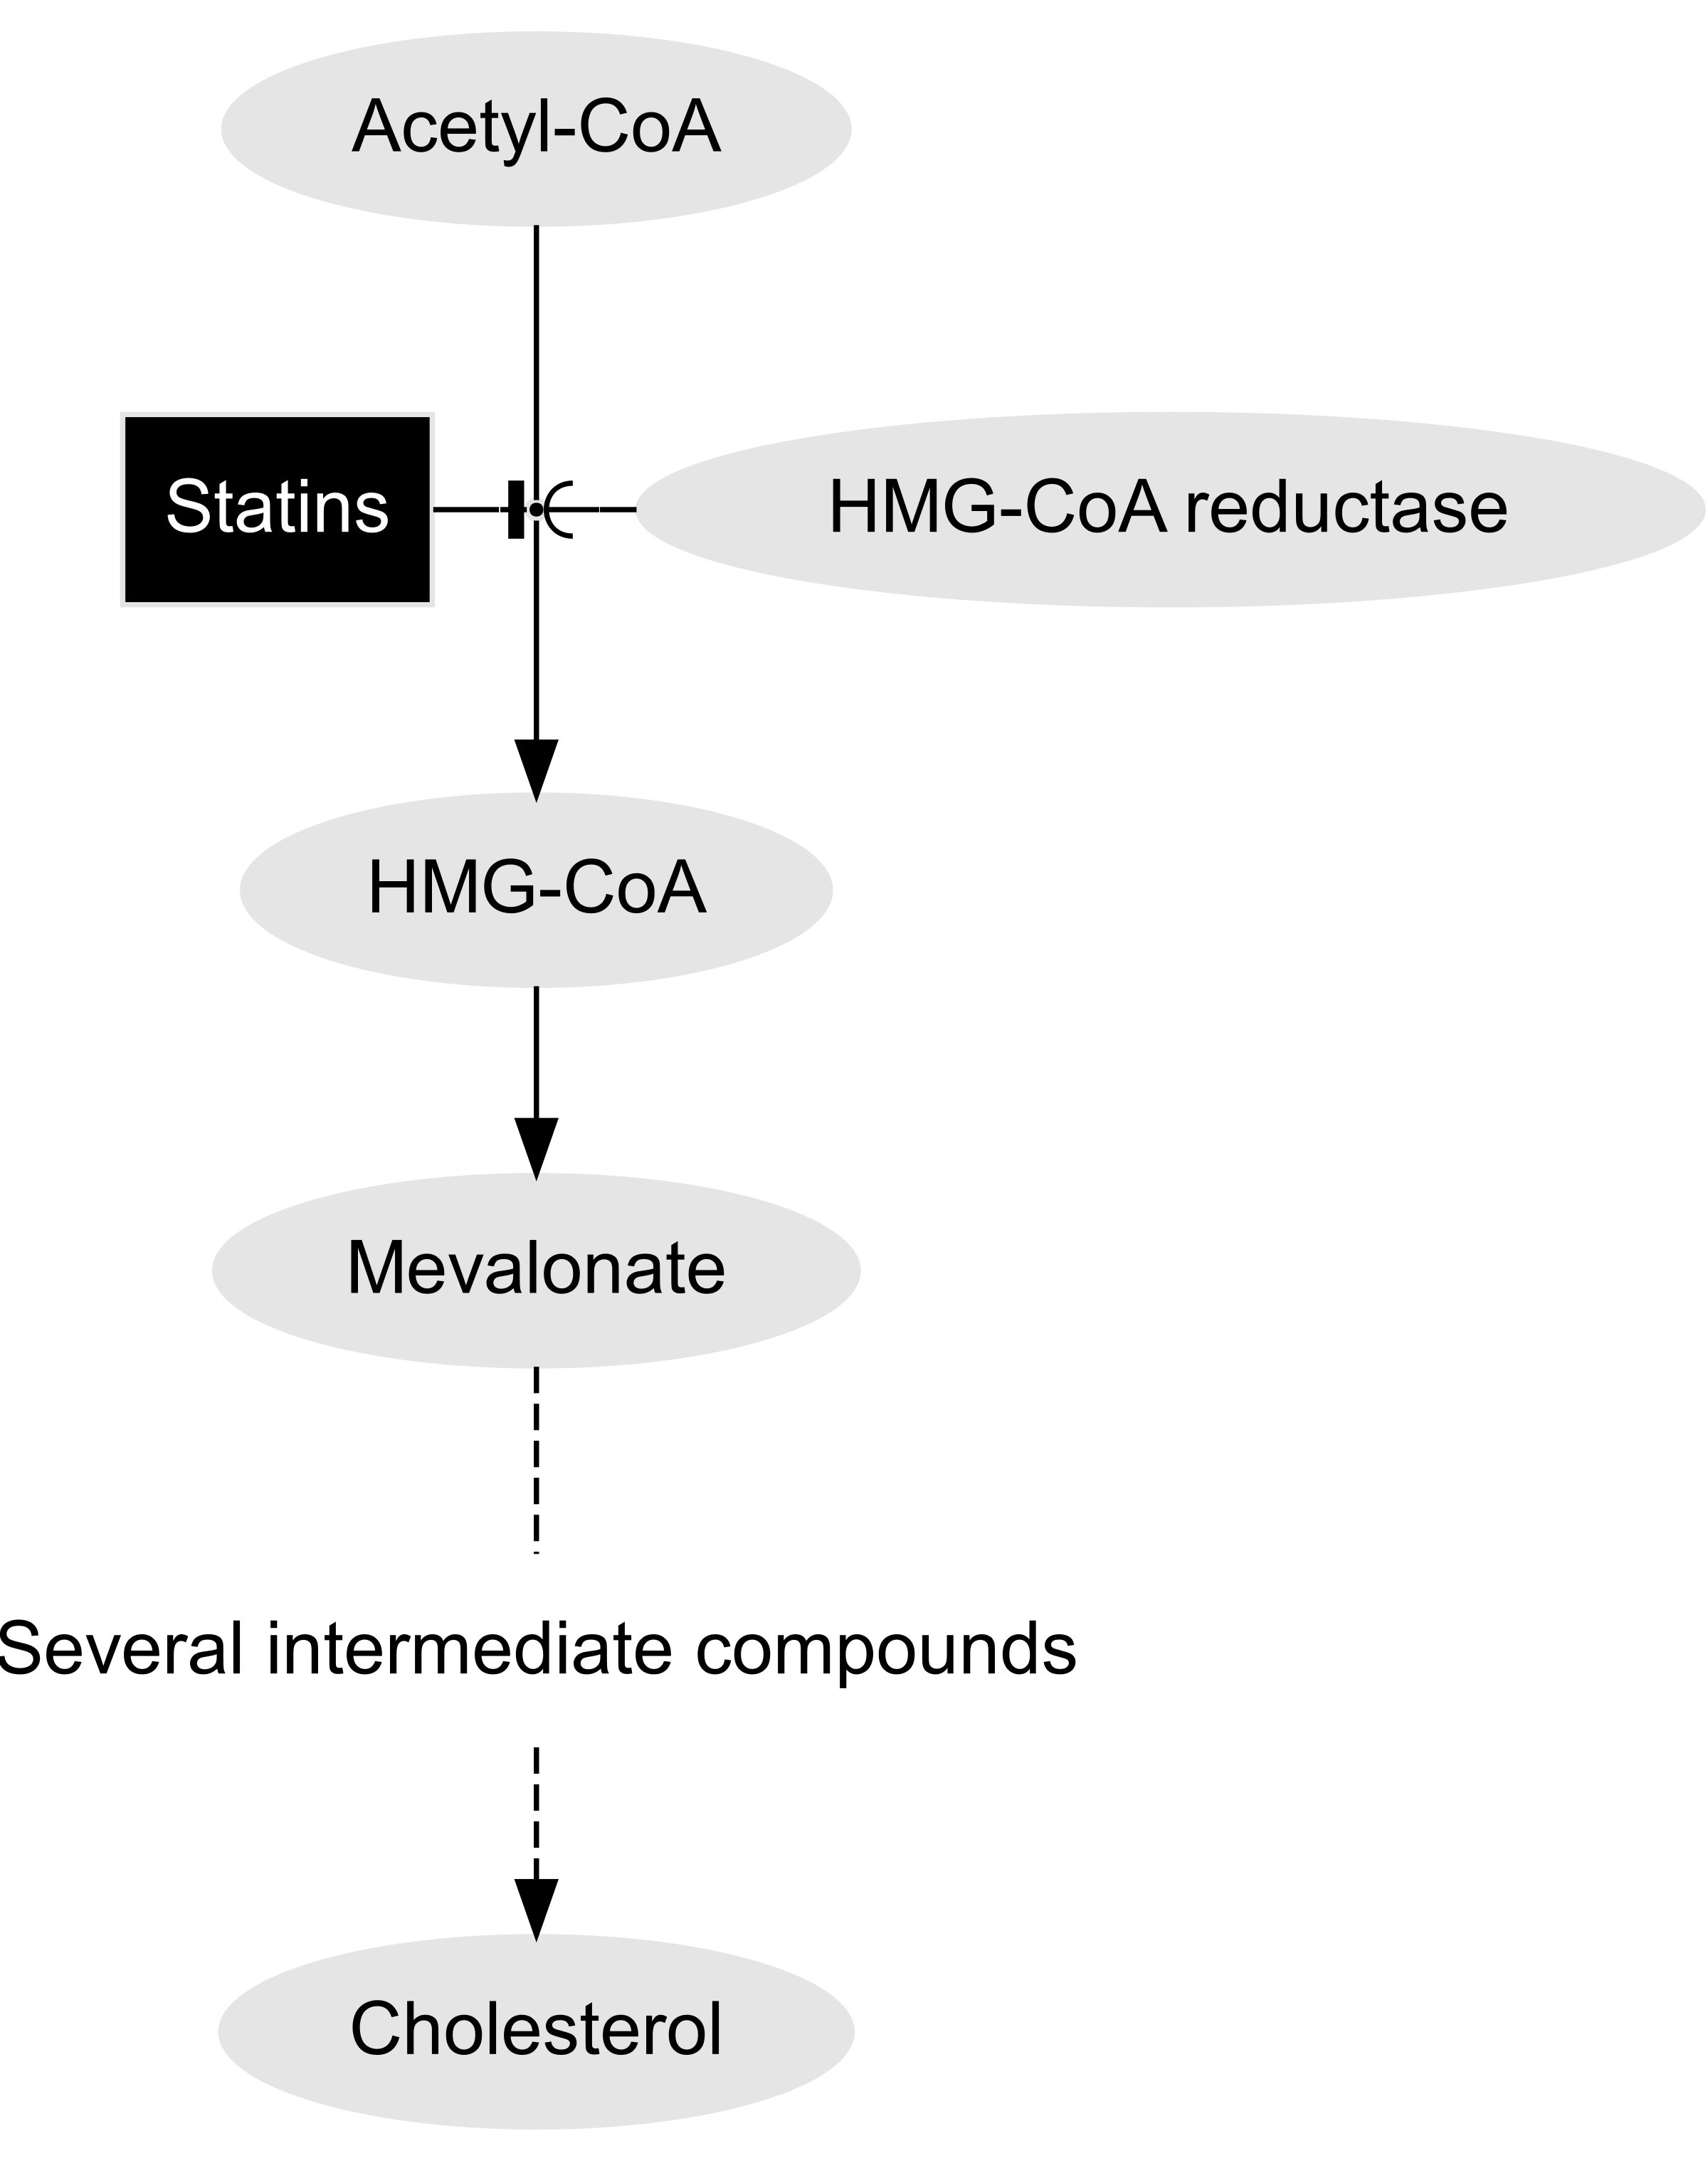
\includegraphics[width=0.5\linewidth]{figures/background/statinPath} 

}

\caption[Statin mechanism of action]{Overivew of statins mechanism of action, inhibiting HMG-CoA reductase which controls the conversion of HMG-CoA to mevalonate, the rate-limiting step in cholesterol biosynthesis.}\label{fig:statin-mechanisam}
\end{figure}

~

Several statin treatments have been widely available for some time (see Table \ref{tab:statinOverview-table}). Depending on the statin and dosage prescribed, the average reduction in LDL-c concentrations ranges from 15\% with low-intensity regimen (e.g.~ravastatin 5 mg/day) up to 60\% with a high-intensity regimen (e.g.~rosuvastatin 80 mg/day).\textsuperscript{\protect\hyperlink{ref-collins2016}{37},\protect\hyperlink{ref-law2003}{38}} Statins also vary with regard to their lipophilicity (the extent to which they are lipid soluble), affecting their localisation within the body, with hydophilic statins being concentrated in the liver and lipophilic statins circulating more widely.\textsuperscript{\protect\hyperlink{ref-schachter2005}{39}} This may create a divide in the pleiotropic affects of statins with differing lipophilicity, particularly given the ability of lipophilic statins to permeate the blood brain barrier.\textsuperscript{\protect\hyperlink{ref-sierra2011}{40}}

~





\begin{table}[H]

\caption[Overview of common statins]{\label{tab:statinOverview-table}Overview of commonly-prescribed statins, summarising their approval date (US), properties and lipid-lowering effect.}
\centering
\begin{tabular}[t]{>{\centering\arraybackslash}p{6em}>{\centering\arraybackslash}p{6em}>{\centering\arraybackslash}p{6em}>{\centering\arraybackslash}p{6em}>{\centering\arraybackslash}p{7.6em}}
\toprule
\textbf{Name} & \textbf{Brand name} & \textbf{Year approved} & \textbf{Properties} & \textbf{Lipid-lowering effect}\\
\midrule
\textbf{Atorvastatin} & Lipitor & 1996 & Lipophilic & +++\\
\midrule
\textbf{Pravastatin} & Lipostat & 1989 & Hydrophilic & +\\
\midrule
\textbf{Rosuvastatin} & Crestor & 2003 & Hydrophilic & ++++\\
\midrule
\textbf{Simvastatin} & Zocor & 1992 & Lipophilic & ++\\
\bottomrule
\end{tabular}
\end{table}

~

\hypertarget{other-lipid-regulating-agents-lra}{%
\subsection{Other lipid regulating agents (LRA)}\label{other-lipid-regulating-agents-lra}}

There are several other interventions that can be used to modify a persons lipid profile, which each acting in slightly different ways (Table \ref{tab}). However, in general, these treatments are either used as adjunct (additional) treatments with statins therapy or are used in situations where statins are contra-indicated or not tolerated.

The most commonly used non-statin therapeutic is ezetimibe,\textsuperscript{\protect\hyperlink{ref-kosoglou2005}{41}} which prevents intestinal absorption of cholesterol. However, when used alone, it has a limited LDL-c lowering effect, leading to the creation of combined statin/ezetimibe therapies (both compounds contained in a single pill, as opposed to complimentary treatments).\textsuperscript{\protect\hyperlink{ref-genest2006}{42}}

Fibrates provide a second example of non-statin therapy. They are used to treat hypertriglyceridaemia by reducing production of triglyceride carrying compounds in the liver. They are commonly used in patients with mixed hyperlipidaemia if treatment with statins has failed to sufficiently control cholesterol levels.

Finally, PCSK9 inhibitors (or PCSK9i) are a relatively new treatment with strong lipid lowering effects, lauded as a potential alternative to statins.\textsuperscript{\protect\hyperlink{ref-chaudhary2017}{43}} Their mechanism of action is to bind to and inhibit PCSK9, which breaks down LDL-c receptors on the surface of the liver, thus allowing more LDL-c to be internalised and broken down.

Other therapies targeting triglycerides exist, including nicotinic acids\textsuperscript{\protect\hyperlink{ref-mckenney2004}{44}} and omega-3-fatty acids,\textsuperscript{\protect\hyperlink{ref-skulas2019}{45}} but they far less effective in LDL-c lowering than the therapies described above.

~



\begin{table}[H]

\caption{\label{tab:lipidTreatments-table}Summary of available treatments for hyperlipidaemia.}
\centering
\begin{tabular}[t]{>{\raggedright\arraybackslash}p{8em}>{\raggedright\arraybackslash}p{8em}>{\raggedright\arraybackslash}p{8em}>{\raggedright\arraybackslash}p{8em}}
\toprule
\textbf{Treatment} & \textbf{Effect} & \textbf{Mechanism of action} & \textbf{Examples}\\
\midrule
\textbf{HMG CoA reductase inhibitors (statins)} & Lowers LDL-c \& TG \newline Raises HDL-c & Inhibits cholesterol biosynthesis pathway in the liver & Atorvastatin, \newline Simvastatin, \newline Pravastatin\\
\midrule
\textbf{Ezetimibe} & Lowers LDL-c & Prevents absorption of cholesterol from diet & \\
\midrule
\textbf{Bile acide sequestrants} & Lowers LDL-c & Prevent bile acid reabsorption in the gastro-intestinal tract, increasing conversion of cholesterol to bile acids & Colestipol\\
\midrule
\textbf{Proprotein convertase subtilisin kexin 9 (PCSK9) inhibitors} & Lowers LDL-c & Bind to PSCK9 protein, preventing it from breaking down LDL receptors on heptatic cells, increasing cholesterol uptake & Evolocumab, \newline Alirocumab\\
\bottomrule
\end{tabular}
\end{table}

~

\hypertarget{evidence-association}{%
\section{Evidence for the association between blood lipids and dementia}\label{evidence-association}}

This section provides an overview of the varying sources of evidence on the relationship between blood lipid levels and dementia risk.

\hypertarget{intro-basic-science}{%
\subsection{Basic science}\label{intro-basic-science}}

A role for lipids in the aetiology of the dementia is supported by both genetic linkage studies and functional cell biology studies. The generation of the amyloid plaques found in the brains of Alzheimer's patients is cholesterol dependent,,\textsuperscript{\protect\hyperlink{ref-burns2003}{46},\protect\hyperlink{ref-mizuno1999}{47}} while the most established genetic risk factor for late-onset dementia, apolipoprotein E (ApoE), is involved in cerebral cholesterol transport. Several other genes involved in cholesterol transport have also been found to be associated with increased AD susceptibility.\textsuperscript{\protect\hyperlink{ref-beecham2014}{48}--\protect\hyperlink{ref-meng2007}{50}}

Despite these results, evidence from the diverse range of epidemiological studies on this topic has been inconclusive.

\hypertarget{observational-studies}{%
\subsection{Observational studies}\label{observational-studies}}

By far the largest source of evidence on the relationship between comes from observational designs. Several studies have examined the relationships between concentrations of serum lipids (total cholesterol (TC), low density lipoprotein cholesterol (LDL-c), high density lipoprotein cholesterol (HDL-c) and triglycerides) and both Alzheimer's disease and vascular dementia and reported extremely varied results. In some studies, a high serum cholesterol concentration has been found to be associated with an increase in susceptibility to AD,\textsuperscript{\protect\hyperlink{ref-kivipelto2002}{51}--\protect\hyperlink{ref-whitmer2005}{55}} however others have shown no association,\textsuperscript{\protect\hyperlink{ref-li2005}{56}--\protect\hyperlink{ref-tan2003}{59}} or a reduced susceptibility.\textsuperscript{\protect\hyperlink{ref-mielke2005}{60},\protect\hyperlink{ref-reitz2004}{61}} With regards vascular dementia, decreased levels of HDL-c appear to be associated with increased risk,\textsuperscript{\protect\hyperlink{ref-reitz2004}{61}} while for LDL-c, studies have reported both positive and negative associations.\textsuperscript{\protect\hyperlink{ref-reitz2004}{61},\protect\hyperlink{ref-moroney1999}{62}}

\hypertarget{randomised-controlled-trials}{%
\subsection{Randomised controlled trials}\label{randomised-controlled-trials}}

In terms of the central research of this thesis, RCTs of statin therapy can be used to provide indirect evidence for the effect of reducing blood LDL-c levels on dementia risk.

However, RCTs may be infeasible if the outcome of interest is one with a long prodomal period, such as dementia (see Section \ref{underlying-pathologies}), as they would require extremely long and costly follow-up.\textsuperscript{\protect\hyperlink{ref-ritchie2015}{63}} It is no surprise then that the two previous trials providing evidence on the effect of statins on dementia risk, identified by a recent Cochrane review,\textsuperscript{\protect\hyperlink{ref-mcguinness2016}{64}} are in fact trials of statins for the prevention of coronary related outcomes.

While being widely cited, these studies have major limitations that reduce their utility as a source of evidence on the effect of statin treatment on in assessing the impact of lipid-lowering treatment on dementia risk. Firstly, there was no clinical cognitive evaluation of patients to determine a dementia outcome. One of the trials, the Prospective Study of Pravastatin in the Elderly (PROSPER) trial,\textsuperscript{\protect\hyperlink{ref-trompet2010}{65}} reported not on dementia outcomes but on the change in cognitive scores over a mean of 3.2 years. As highlighted in Section \ref{diagnostic-criteria}, a ``change in score'' alone is insufficient to diagnose a dementia outcome. The second trial, the Medical Research Council/British Health Foundation Protection Study,\textsuperscript{\protect\hyperlink{ref-heartprotectionstudycollaborativegroup2002}{66}} found no effect of simvastatin on dementia (OR: 1.00, 95\%CI: 0.61-1.65), but did not report how the outcome was assessed/recorded within the trial.

Additionally, the two trials did not make any effort to assign an underlying pathology to each case, instead reporting an all-cause dementia outcome. As discussed in Section \ref{underlying-pathologies}, the different underlying pathology of dementia have different mechanisms of action, and so it is not gauranteed that the effect of statins would be consistent across them.

Both trials were also limited by the relatively short follow-up period examined, expected when the primary outcome of the trials were coronary related conditions rather than dementia.\textsuperscript{\protect\hyperlink{ref-trompet2010}{65},\protect\hyperlink{ref-heartprotectionstudycollaborativegroup2002}{66}} The PROSPER trial had a mean follow-up of 3.2 years, while the MRC/BHF Protection Study estimated risk at 5 years of follow-up. Given the long lag time between non-symptomatic onset of dementia and clinical presentation, it is likely that these durations are insufficient to fully capture the onset of dementia. Finally, as they included only patients at high vascular risk, their generalisability to other settings is limited.\textsuperscript{\protect\hyperlink{ref-mcguinness2016}{64}}

\hypertarget{mendelian-randomisation}{%
\subsection{Mendelian randomisation}\label{mendelian-randomisation}}

Newer methodological approaches, such as Mendelian randomisation (MR),\textsuperscript{\protect\hyperlink{ref-daveysmith2014}{67}} have also been used to examine the effect of varying lipid levels on dementia risk in an effort to combat the risk of reverse causation and residual confounding inherent to observational studies.\textsuperscript{\protect\hyperlink{ref-greenland2000}{68}} In brief, MR uses genetic variants that are both strongly associated with the exposure of interest and are independent from potential confounders to strengthen causal inference.\textsuperscript{\protect\hyperlink{ref-daveysmith2014}{67}} The analytic method relies on several assumptions about the instrumental variable (IV),\textsuperscript{\protect\hyperlink{ref-davies2018}{69}} namely that:

\begin{enumerate}
\def\labelenumi{\arabic{enumi}.}
\tightlist
\item
  the IV is associated with the exposure of interest (the relevance assumption);
\item
  the IV and outcome do not share a common cause (the independence assumption); and
\item
  the IV does not affect the outcome other than via the exposure (the exclusion restriction assumption).
\end{enumerate}

Recent MR studies indicated that genetically determined low levels of LDL-c may cause a reduction in AD risk.\textsuperscript{\protect\hyperlink{ref-larsson2017}{70},\protect\hyperlink{ref-ostergaard2015}{71}} However, the effect was attenuated in sensitivity analysis that exclude the region surrounding the ApoE gene, the strongest known risk factor for Alzheimer's disease.\textsuperscript{\protect\hyperlink{ref-kim2009}{72}} Inclusion of ApoE4 variants invalidates the exclusion restriction criteria (Assumption 3, above), as the risk reduction observed may be driven by variants in this region via a pathway independent of lipid levels. This was supported by further MR studies where \emph{ApoE4} variants were intentionally excluded.\textsuperscript{\protect\hyperlink{ref-benn2017}{73}}

Despite the increasing number of MR studies examining this topic, no systematic review of this study design as a source of evidence has been performed.

~

In summary, multiple sources of evidence exist on the relationship between statins and dementia. In the next section, I introduce the synthesis of diverse sources of evidence as the theoretical framework used in this thesis.

\hypertarget{theoretical-framework-evidence-synthesis}{%
\section{Theoretical framework: Evidence synthesis}\label{theoretical-framework-evidence-synthesis}}

Evidence synthesis is the process of finding and integrating information from several sources to examine a research question.\textsuperscript{\protect\hyperlink{ref-donnelly2018}{74}} A common tyoe of evidence synthesis is a systematic review, either with or without a meta-analysis.\textsuperscript{\protect\hyperlink{ref-chandler2019chapter}{75}}

The results of an evidence synthesis exercise can be used to provide a more definitive answer to that question or, failing that, to highlight gaps in the existing evidence base. The ability to identify these gaps is particularly useful in guiding future research to address questions that have yet to be answered.

This thesis seeks to use an evidence synthesis framework to assess the effect of lipids, and treatments that influence lipid levels, on dementia outcomes.
Specifically, this thesis considers three concepts within the umbrella term of evidence synthesis:

\begin{itemize}
\tightlist
\item
  Inclusion of preprints
\item
  Triangulation across evidence sources
\item
  Individual patient data meta-analysis
\end{itemize}

These three elements are expanded on below and are used to frame the research presented in the subsequent Chapters.

\hypertarget{diverse-sources-preprints}{%
\subsection{Inclusion of preprints}\label{diverse-sources-preprints}}

The importance of including grey (or gray) literature in systematic reviews is widely acknowledged. Meta-research studies have demonstrated that systematic reviews excluding grey literature sources overestimate the effect of interventions.\textsuperscript{\protect\hyperlink{ref-conn2003}{76}--\protect\hyperlink{ref-hopewell2007}{78}} Common, well-accepted forms of grey literature include conference abstracts and theses.\textsuperscript{\protect\hyperlink{ref-lefebvre2019searching}{79}}

A important developing source of grey literature are preprints. Defined by the Committee on Publication Ethics (COPE) as `scholarly manuscript{[}s{]} posted by the author(s) in an openly accessible platform, usually before or in parallel with the peer review process'\textsuperscript{\protect\hyperlink{ref-committeeonpublicationethicscope2018}{80}}, preprints serve several purposes. They are used to establish primacy when submitting to a journal where the peer-review process may take several months,\textsuperscript{\protect\hyperlink{ref-vale2016}{81}} to rapidly disseminate research findings, as occurred during the COVID-19 pandemic,\textsuperscript{\protect\hyperlink{ref-fraser2020preprinting}{82}} and to make available publications that may not have been accepted elsewhere in an attempt to combat publication bias or the ``file-drawer'' effect.\textsuperscript{\protect\hyperlink{ref-rosenthal1979}{83}}

One of the major criticisms of using preprints as an evidence source is that they have not yet undergone formal peer review.\textsuperscript{\protect\hyperlink{ref-maslove2018}{84},\protect\hyperlink{ref-schalkwyk2020}{85}} However, this approach assigns substantial weight to peer-review as a indicator of ``quality'', and is at odds with the acceptance of non-reviewed conference proceedings as an evidence source.\textsuperscript{\protect\hyperlink{ref-lefebvre2019searching}{79},\protect\hyperlink{ref-mahood2014}{86}} The argument for including preprints as an evidence source is further strengthened by results that demonstrate preprinted studies seldom change following peer review. Meta-studies of the concordance between preprinted and published studies showed that results were broadly comparable between the two, indicating that while the numerical results may change, the overall interpretation of the results were consistent in the majority of cases.\textsuperscript{\protect\hyperlink{ref-shi2021}{87}--\protect\hyperlink{ref-nicholson2021}{89}} This indicates that preprints should be considered a reliable reflection of a given study.

In this thesis, preprints are considered an important source of evidence, in contrast to previous reviews on this topic. However, as with many sources of grey literature,\textsuperscript{\protect\hyperlink{ref-mahood2014}{86}} there are several logistical issues with carrying out systematic searches in preprint repositories. As such, to enable the inclusion of preprints in the systematic review described in Chapters \ref{sys-rev-methods-heading}, a new tool addressing these issues is presented in Chapter \ref{sys-rev-tools}.

\hypertarget{intro-triangulation}{%
\subsection{Triangulating across study designs}\label{intro-triangulation}}

As illustrated in Section \ref{evidence-association}, several diverse epidemiological methods have been used to examine the effect of varying blood lipid levels on dementia risk. However, each method is limited by its own biases. Aetiological triangulation is a developing evidence synthesis method that seeks to exploit these inherent differences in study design, and as a result, in biases.\textsuperscript{\protect\hyperlink{ref-lawlor2016}{90}} If several sources of evidence are available and point towards identical conclusions about an exposure-outcome relationship, and these sources are at risk of unrelated biases, this strengthens our confidence in the result. The ideal scenario is where predicted sources of bias are likely to be in competing directions, strengthen the effect of the exposure and the other to attenuate it.\textsuperscript{\protect\hyperlink{ref-lawlor2016}{90}} As such, triangulating these results can provides us a middle-ground between the competing directions of bias. A triangulation approach can also prove useful in a prospective manner, helping to design new studies that are at risk of different sources of bias to that already available from the published literature.\textsuperscript{\protect\hyperlink{ref-munafo2018}{91}}

This thesis seeks to apply a triangulation approach to provide the best available evidence on the effect of lipids, and lipid regulating agents, on dementia outcomes.

All existing evidence, regardless of study design, is first identified by the by the systematic review presented inChapters \ref{sys-rev-methods-heading}/\ref{sys-rev-results-heading}. Risk-of-bias assessment using a domain-based tool is already a recommended part of the systematic review process, but is particularly important to a triangulation exercise.\textsuperscript{\protect\hyperlink{ref-page2021}{92}--\protect\hyperlink{ref-mcguinness2018}{94}} As such, a core component of the review is a comprehensive domain-based risk-of-bias assessment for all included studies.

Finally all evidence, both pre-existing and produced as part of this thesis (Chapter \ref{cprd-analysis-heading} and \ref{ipd-analysis-heading}), are triangulated in Chapter \ref{dicussion-heading}.

\hypertarget{individual-patient-data-meta-analysis}{%
\subsection{Individual patient data meta-analysis}\label{individual-patient-data-meta-analysis}}

Individual patient data meta-analyses are commonly held to represent the gold standard in evidence synthesis methodology.\textsuperscript{\protect\hyperlink{ref-riley2010}{95},\protect\hyperlink{ref-stewart1993}{96}} IPD methods seek to obtain the raw data from each study identified in a systematic review, rather than basing the meta-analysis on summary results extracted from the literature.\textsuperscript{\protect\hyperlink{ref-riley2010}{95}}

In the context of this thesis, if lipids are found to have a causal role in development of dementia, evidence-based preventative strategies would be best informed by identifying the types of individuals who are most likely to receive benefit from treatment with lipid-modifying agents.\textsuperscript{\protect\hyperlink{ref-arain2009}{97}--\protect\hyperlink{ref-mccartney2016}{99}} However, if primary studies do not present results stratified by covariates of interest, meta-analyses of summary-level data on this topic often have limited ability to examine research questions related to exposure-covariate interactions.\textsuperscript{\protect\hyperlink{ref-riley2010}{95}} In terms of this thesis, patient sex is considered to be of particular interest.\textsuperscript{\protect\hyperlink{ref-arain2009}{97},\protect\hyperlink{ref-letenneur1999}{100}}

An IPD meta-analysis of lipid levels on dementia outcomes would overcome this limitation of summary-level data, as access to the raw data allows for an analysis that investigates these interactions.\textsuperscript{\protect\hyperlink{ref-riley2020}{101}} This approach has the added benefit of allowing a common set of inclusion criteria and statistical model to be applied across all datasets, potentially eliminating some important sources of heterogeneity.\textsuperscript{\protect\hyperlink{ref-stewart2002}{102}}

Despite their advantages, IPD meta-analysis are rarely performed.\textsuperscript{\protect\hyperlink{ref-tugwell2010}{103}} Factors limiting their uptake include the increased time and effort they require when compared to a summary-level analysis, and the low success rate associated with obtaining the raw data.\textsuperscript{\protect\hyperlink{ref-nevitt2017}{104},\protect\hyperlink{ref-ventresca2020}{105}} The data underlying primary studies are frequently not publicly available,\textsuperscript{\protect\hyperlink{ref-alsheikh-ali2011}{106},\protect\hyperlink{ref-federer2018}{107}} and the availability of data ``available on request from authors'' declines rapidly over time.\textsuperscript{\protect\hyperlink{ref-vines2014}{108}} Several systematic barriers to open data sharing have been identified\textsuperscript{\protect\hyperlink{ref-vanpanhuis2014}{109}}. Of particular concern for biomedical IPD analyses are legal issues surrounding the sharing of medical data, motivated by concerns around patient privacy.\textsuperscript{\protect\hyperlink{ref-wartenberg2010}{110}}

In response to these limitations, new collaborative initiatives have developed to enable rapid access to relevant data in a secure supported workshop. The most import in relation to this thesis is the Dementia Platform UK (DPUK),\textsuperscript{\protect\hyperlink{ref-bauermeister2020}{111}} which aims to provide access to several dementia-related datasets via a single simplified application process.

I will will attempt to obtain the raw data from relevant primary studies identified by the systematic review in Chapters \ref{sys-rev-methods-heading}/\ref{sys-rev-results-heading}. Any data obtained will be combined with that available from the DPUK portal as part of an individual participant data meta-analysis in Chapter \ref{ipd-analysis-heading}, enabling the assessment of the effect of lipids on dementia stratified by key variables such as sex.

\hypertarget{background-thesis-overview}{%
\section{Thesis overview}\label{background-thesis-overview}}

\hypertarget{aims-and-objectives}{%
\subsection{Aims and objectives}\label{aims-and-objectives}}

The over-arching aim of this thesis is to explore the relationship between blood lipid levels, and by extension treatments that modify blood lipid levels such as statins, and the subsequent risk of dementia and related outcomes

The specific research objectives that this thesis seeks to address are:

\begin{itemize}
\tightlist
\item
  To create a tool that allows for the inclusion of health related preprints in evidence syntheses in a systematic and reproducible manner
\item
  To review all available evidence across multiple diverse study designs to assess the effect of lipids and lipid regulating agents on dementia risk
\item
  To examine whether there is evidence for an effect of lipid-regulating agents on dementia and related outcomes in a large scale population-based cohort, the Clinical Practice Research Datalink (CPRD)
\item
  To meta-analyse raw dementia-related datasets as part of a individual participant data (IPD meta-analysis) to produce evidence on exposure-covariate interactions
\item
  To propose a generalised framework for the quantitative triangulation across diverse evidence sources
\end{itemize}

\hypertarget{thesis-structure}{%
\subsection{Structure}\label{thesis-structure}}

Chapters are self-contained, presenting the methods and results of that specific research project. They are bookended by introductory and discussion sections which place the methods and results in context. Each chapter is prefaced by a ``Lay'' or plain English summary, developed with input from the Patient and Public Advisory Group (see Section \ref{disc-PPI} for a discussion of the group's involvement and Appendix \ref{appendix-ppi} for more detail on the group).

\begin{itemize}
\tightlist
\item
  \textbf{Chapter \ref{background-heading}:} Background information on dementia and blood lipid levels. This chapter provides an introduction to the topics covered in this thesis to non-subject area experts, and discusses the motivation for the remainder of the thesis.
\item
  \textbf{Chapter \ref{sys-rev-tools-heading}:} This Chapter introduces a new tool, \texttt{medrxivr}, which was used to developed to allow for systematic searches of the health-related preprint repositories.
\item
  \textbf{Chapters \ref{sys-rev-methods-heading}/\ref{sys-rev-results-heading}:} These Chapters describe, respectively, the methods and results of a comprehensive systematic review and meta-analysis. This review examined all available evidence on the effect of blood lipids, and interventions that modified blood lipids, on dementia outcomes.
\item
  \textbf{Chapter \ref{cprd-analysis-heading}:} This Chapter examines the relationship between lipid-regulating agent use and dementia outcomes in the Clinical Practice Research Datalink, a large primary care electronic health record database.
\item
  \textbf{Chapter \ref{ipd-heading}:} This Chapter describes an individual patient data analysis of several longitudinal cohort studies to describe the relationship between blood serum lipids and dementia outcomes, stratified by important covariates such as sex.
\item
  \textbf{Chapter \ref{discussion-heading}}: This Chapter integrates the diverse evidence identified by, and produced as part of, this thesis. The overall strengths and weaknesses of this project are discussed in detail, and further avenues of research are suggested.
\end{itemize}

\hypertarget{thesis-output}{%
\section{Outputs from this thesis}\label{thesis-output}}

The outputs of this thesis are detailed below, and include peer-reviewed papers, presentations, and open-source evidence synthesis tools.

\hypertarget{contributions-to-the-scientific-literature}{%
\subsection{Contributions to the scientific literature}\label{contributions-to-the-scientific-literature}}

During the course of this thesis, I have made several contributions to the scientific literature. Those arising from or directly related to the contents of this submission are presented below.

~

\emph{\textbf{McGuinness, L. A.}, and L Schmidt. (2020) medrxivr: Accessing and searching medRxiv and bioRxiv preprint data in R. Journal of Open Source Software 5.54 2651. DOI: \href{https://doi.org/10.21105/joss.02651}{10.21105/joss.02651}}

A paper introducing the open-source preprint search tool described in Chapter \ref{sys-rev-tools-heading}. As is common for journal articles describing software, the paper is intentionally short providing only a broad overview of the tool while extensive documentation is available from the project website (see Section \ref{sys-rev-tools-intro} for more details).

~

\emph{Hennessy, E. A., Acabchuk, R., Arnold, P. A., Dunn, A. G., Foo, Y. Z., Johnson, B. T., Geange, S. R., Haddaway, N. R., Nakagawa, S., Mapanga, W., Mengersen, K., Page, M., Sánchez-Tójar, A. Welch, V., \textbf{McGuinness L. A.} (2021). Ensuring Prevention Science Research is Synthesis-Ready for Immediate and Lasting Scientific Impact. Prevention Science . DOI: \href{https://doi.org/10.1007/s11121-021-01279-8}{10.1007/s11121-021-01279-8}}

The experience of extracting data for the systematic review in Chapters \ref{sys-rev-methods-heading}/\ref{sys-rev-results-heading} inspired a practical guide for researchers. This piece was co-written with Dr.~Emily Hennessy (see Author Declarations in the front materials).

~

\emph{\textbf{McGuinness, L. A.}, and Higgins J. P. T. (2020) ``Risk‐of‐bias VISualization (robvis): An R package and Shiny web app for visualizing risk‐of‐bias assessments.'' Research Synthesis Method). DOI: \href{https://doi.org/10.1002/jrsm.1411}{10.1002/jrsm.1411}}

The tool used to visualise the risk-of-bias assessments in Chapters \ref{sys-rev-methods-heading}/\ref{sys-rev-results-heading} has been published in Research Synthesis Methods. See Appendix \ref{appendix-robvis} for more details on this tool. Note that this publication does not describe the recently-developed functionality for producing bias direction plots, as described in Chapter \ref{tri-heading}.

~

\emph{\textbf{McGuinness, L. A.}, and Sheppard A. L. 2020. ``A Descriptive Analysis of the Data Availability Statements Accompanying Medrxiv Preprints and a Comparison with Their Published Counterparts.'' PLOS ONE 16(5): e0250887. DOI: \href{https://doi.org/10.1371/journal.pone.0250887}{10.1371/journal.pone.0250887}}

Using the tool described in Chapter \ref{sys-rev-tools}, I lead a ``research-on-research'' study to assess the concordance between the openness of data availability statements accompanying a sample of medRxiv preprints and their published counterparts.

~

For information on additional contributions to the scientific literature not directly related to this thesis, see Appendix \ref{appendix-publications}.

~

\hypertarget{presentationstalks}{%
\subsection{Presentations/Talks}\label{presentationstalks}}

\emph{``Identifying and triangulating all available evidence on the effect of blood lipids and statins on dementia outcomes''}: Poster presentation, Alzheimer's Association International Conference 2021.
~

\emph{``medrxivr: A new tool for searching for and retrieving records and PDFs from the medRxiv preprint repository''}: Accepted oral presentation abstract, Cochrane Colloquium 2020 (note: event was cancelled due to the COVID-19 pandemic)

~

\emph{``On the shoulders of giants'': advantages and challenges to building on established evidence synthesis packages, using the \{robvis\} package as a case study"}: Oral presentation, Evidence Synthesis and Meta-Analysis in R Conference (ESMARConf) 2021.

~

\emph{``RoB 2.0: A revised tool to assess risk of bias in randomized trials''}: Webinar, co-presented with Dr.~Theresa Moore as part of the Evidence Synthesis Ireland Methods Series.

\hypertarget{outputs-software}{%
\subsection{Software}\label{outputs-software}}

\textbf{\texttt{medrxvir}}

An R package that allows users to easily search and retrieve bibliographic data from the medRxiv\textsuperscript{\protect\hyperlink{ref-rawlinson2019}{112}} and bioRxiv\textsuperscript{\protect\hyperlink{ref-sever2019}{113}} preprint repositories. See Chapter \ref{sys-rev-tools-heading} for more details. Install a stable version of the package from the Comprehensive R Archive Network (CRAN), or alternatively install the development version from GitHub, using:

\begin{Shaded}
\begin{Highlighting}[]
\CommentTok{\# CRAN version}
\FunctionTok{install.packages}\NormalTok{(}\StringTok{"medrxivr"}\NormalTok{)}

\CommentTok{\# Development version}
\NormalTok{devtools}\SpecialCharTok{::}\FunctionTok{install\_github}\NormalTok{(}\StringTok{"ropensci/medrxivr"}\NormalTok{)}
\end{Highlighting}
\end{Shaded}

~

\textbf{\texttt{robvis}}

An R package and associated \texttt{shiny} web application that allows users to easily visualize the results of the risk-of-bias assessments performed as part of a systematic review. See Appendix \ref{appendix-robvis} for more details. Install a stable version of the package from CRAN, or alternatively install the development version from GitHub, using:

\begin{Shaded}
\begin{Highlighting}[]
\CommentTok{\# CRAN version}
\FunctionTok{install.packages}\NormalTok{(}\StringTok{"robvis"}\NormalTok{)}

\CommentTok{\# Development version}
\NormalTok{devtools}\SpecialCharTok{::}\FunctionTok{install\_github}\NormalTok{(}\StringTok{"mcguinlu/robvis"}\NormalTok{)}
\end{Highlighting}
\end{Shaded}

~

\hypertarget{summary}{%
\section{Summary}\label{summary}}

This Chapter has provided background information on the core elements of the central research question, framed the research presented in this thesis in the context of an evidence synthesis framework, and described the contributions of this thesis to the scientific literature.

\newpage

\hypertarget{references}{%
\section{References}\label{references}}

\begin{savequote}
Why are open source statistical programming\\
languages the best?

Because they R.
\qauthor{--- Chris Beely, 2013\textsuperscript{\protect\hyperlink{ref-beely2013}{114}}}\end{savequote}



\hypertarget{sys-rev-tools-heading}{%
\chapter{medrxivr: an R package for systematically searching biomedical preprints}\label{sys-rev-tools-heading}}

\minitoc 

\hypertarget{lay-summary-1}{%
\section{Lay summary}\label{lay-summary-1}}

Preprints are copies of academic manuscripts that are posted online in advance of being formally published by an academic journal. They represent an important source of scientific literature. A new software program called \texttt{medrxivr} was created to allow researchers to find preprints related to their research in a transparent and reproducible way. Development of this tool was an essential part of this thesis, as preprints represent a key source of information needed for the research reported in future chapters.

\hypertarget{sys-rev-tools-intro}{%
\section{Introduction}\label{sys-rev-tools-intro}}

Preprints represent an increasingly important source of scientific information (see Section \ref{diverse-sources-preprints}). As a result, repositories of preprinted articles should be considered a distinct but complementary information source when reviewing the evidence base as part of a systematic review. The two key repositories in the health science are bioRxiv, established in 2013,\textsuperscript{\protect\hyperlink{ref-sever2019}{113}} and medRxiv, which launched in 2019 and was designed to replace the ``Epidemiology'' and ``Clinical Trial'' categories of bioRxiv.\textsuperscript{\protect\hyperlink{ref-rawlinson2019}{112}}

Searching these preprints as part of the systematic review described in Chapter \ref{sys-rev-heading} was a necessity, as many of the existing reviews on the topic of lipids and dementia have not considered this important source of evidence. At the time of writing, however, the bioRxiv and medRxiv websites allow only simple search queries as opposed to the often complex Boolean logic (AND/OR/NOT) that information specialists use to query other major databases.\textsuperscript{\protect\hyperlink{ref-bramer2018}{115},\protect\hyperlink{ref-gusenbauer2020}{116}} Additionally, the best available extraction mechanism for obtaining references for all records returned by a search were to go through each record, one-by-one, downloading individual citations. As the scale of these preprint databases increase, particularly in light of the massive expansion of the medRxiv repository as a result of COVID, this already time-consuming and error-prone method is no longer feasible.

This chapter outlines the development and key functionality of \texttt{medrxivr} (version 0.0.5), a tool I created to facilitate the systematic searching of medRxiv and bioRxiv preprints. The factors that necessitated the development of this tool in the context of this thesis are outlined, and the use of \texttt{medrxivr} in my own projects and by other researchers is discussed. As the majority of work on this aspect of my thesis is represented by lines of code or online documentation (available at \url{https://github.com/ropensci/medrxivr} and \url{https://docs.ropensci.org/medrxivr/} respectively), this chapter is an intentionally short, high-level summary of my work on this project. The GitHub repository for the \texttt{medrxivr} contains a complete record of the development of this tool, including discussion with other members of the systematic review community.\textsuperscript{\protect\hyperlink{ref-zotero-15029}{117}}

~





\begin{figure}

{\centering 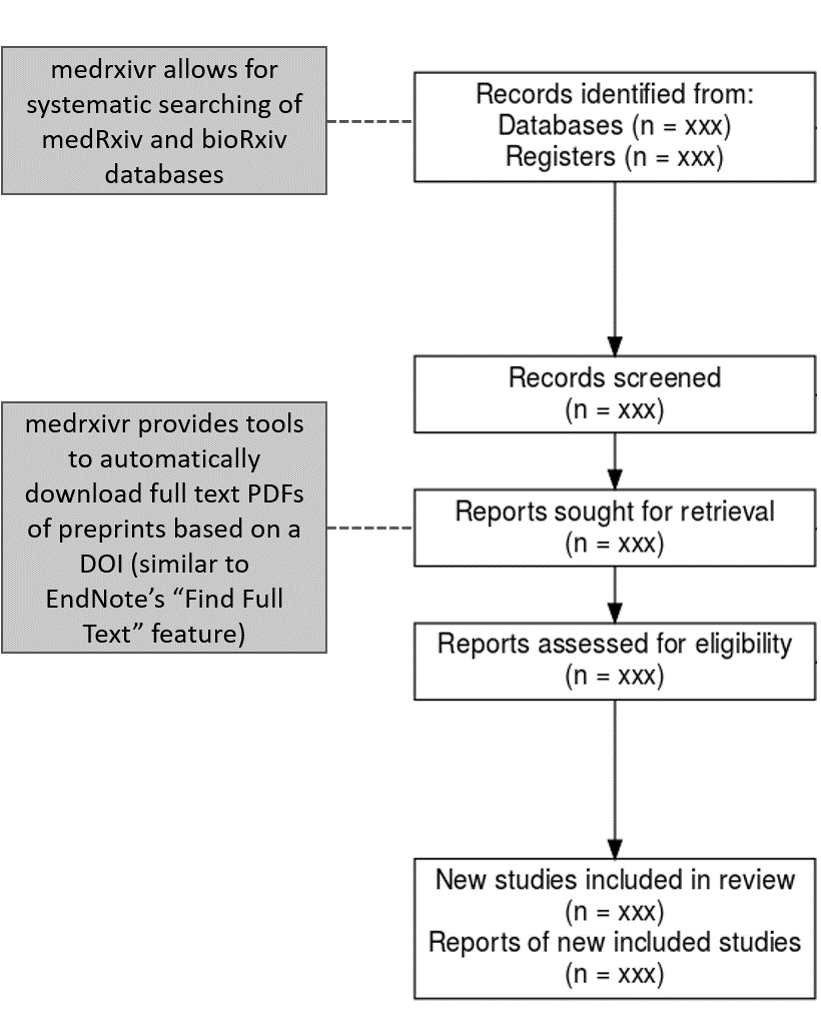
\includegraphics[width=0.65\linewidth]{figures/sys-rev-tools/medrxiv-role} 

}

\caption[Role of \texttt{medrxivr} in a systematic review workflow]{\textbf{Role of \texttt{medrxivr} in a systematic review workflow} - \texttt{medrxivr} allows for systematic searching of biomedical preprints as part of the initial literature searching. Following title and abstract screening, reviewers can then programmatically retrieve a copy of the PDF of included records to facilitate the full-text screening stage (similar to Endnote's ``Find Full Text'' feature).}\label{fig:medrxivr-sr}
\end{figure}

\hypertarget{development}{%
\section{Development}\label{development}}

\hypertarget{success-criteria}{%
\subsection{Success criteria}\label{success-criteria}}

I developed the tool to meet three success criteria,\textsuperscript{\protect\hyperlink{ref-wateridge1995}{118}} influenced both by the functionality required to perform systematic searches as part of the review in Chapter \ref{sys-rev-heading}, discussion with information specialist colleagues, and an informal survey of the evidence synthesis and health librarian communities on Twitter. The criteria were as follows:

\begin{enumerate}
\def\labelenumi{\arabic{enumi}.}
\item
  reliable, reproducible and transparent search functionality, allowing for Boolean (AND/OR/NOT) operator logic;
\item
  support for bulk export of references returned by the search to a file type that can be readily imported into a reference manager (e.g., \emph{.bib} or \emph{.ris}); and
\item
  automated retrieval of the full-text PDFs of relevant records, similar to the Find Full Text feature offered by EndNote.
\end{enumerate}

~

\hypertarget{alternative-medrxivbiorxiv-interfaces}{%
\subsection{Alternative medRxiv/bioRxiv interfaces}\label{alternative-medrxivbiorxiv-interfaces}}

Prior to development of this tool, I conducted an audit of existing tools for accessing medRxiv and bioRxiv metadata. While none address the success criteria described above, two of these tools are useful to consider to highlight the additional functionality that \texttt{medrxivr} contributes.

The first, a platform called Rxivist\textsuperscript{\protect\hyperlink{ref-abdill2019}{119}}, allows users to search preprints using keywords. However, the core functionality of the Rxivist platform is focused around exploring the number of times a preprint has been downloaded and/or shared on Twitter, to allow researchers to find the most popular papers related to their topic. The search interface\textsuperscript{\protect\hyperlink{ref-zotero-15027}{120}} does not allow for complex search strategies using Boolean operators and there is no option to batch-export the results of a search.

The second tool, \texttt{search.bioPreprint}, allows users to search for terms across a range of preprint servers, including medRxiv and bioRxiv, but also journals which use a post-publication peer-review process such as F1000Research.\textsuperscript{\protect\hyperlink{ref-iwema2016}{121}} However, similar to the Rxivist platform, this tool is designed for researchers aiming to keep up to date with recent developments in their fields rather than systematically assess the entirety of the available literature. As such, the platform only returns the most recent 1,000 records by publication date.

Finally, neither tool provides an easy way to programmatically download a copy of the PDF of relevant preprints as part of the preparation for the full-text screening stage of a systematic review.

~

\hypertarget{early-versions}{%
\subsection{Early versions}\label{early-versions}}

Work on the \texttt{medrxivr} tool began in Summer 2019, and initially consisted of a development of set of R scripts to allow for searching medRxiv and bioRxiv as part of the systematic search outlined in Chapter \ref{sys-rev-heading}. Following interest from other researchers in using the \emph{ad-hoc} web-scraping scripts, additional development work took place in 2019/2020, allowing for improved searching and exporting functionality and I released the initial version of the \texttt{medrxivr} R package in February 2020.

Early versions of the tool had a reliance on scraping data directly from the repository website. Web-scraping is a fragile mechanism for extracting data, as it is entirely dependent on consistent website design and underlying code structure remaining unchanged.\textsuperscript{\protect\hyperlink{ref-shaw2002}{122},\protect\hyperlink{ref-laprie1992}{123}}. In the case of \texttt{medrxivr}, as the medRxiv/bioRxiv websites are regularly updated, ensuring the web-scraping performed as expected required me to regularly update or fix the script.

However, an Application Programming Interface (API) for the medRxiv and bioRxiv repositories was made public in early 2020 by the institution responsible for managing these preprint repositories, the Cold Springs Harbor Laboratory. This allowed for newer versions of the \texttt{medrxivr} package to engage in active ``fault prevention'' and provide a more robust interface to the data by removing the reliance of web-scraping.\textsuperscript{\protect\hyperlink{ref-laprie1992}{123}}

~

\hypertarget{package-infrastructure}{%
\subsection{Package infrastructure}\label{package-infrastructure}}

I wrote the \texttt{medrxvir} package in R using RStudio,\textsuperscript{\protect\hyperlink{ref-rcoreteam2019}{124}} and followed development best-practice, including development of detailed documentation, a robust unit testing framework (99\% of all code lines within the package are formally tested across multiple platforms including Windows, MacOS, and Linux), and in-depth code review by two experienced, independent reviewers.

~

\hypertarget{usage}{%
\section{Usage}\label{usage}}

The \texttt{medrxivr} R package is split into two component parts:

\begin{itemize}
\tightlist
\item
  an interface to the Cold Springs Harbor Laboratory API, which imports medRxiv and bioRxiv metadata into R; and
\item
  a collection of functions for working with the imported metadata, with an explicit focus on searching this data as part of a systematic review or evidence synthesis project.
\end{itemize}

The standard workflow is to download a copy of all metadata contained in the repository, and then to perform searches on this local copy. This is a workaround as the Cold Springs Harbor Laboratory API does not provide any functionality to search the database.

While the package allows users to interact with and search both medRxiv and bioRxiv metadata, as the process is identical for both, searching the medRxiv database is used as an illustrative example throughout this chapter.

~

\hypertarget{installation}{%
\subsection{Installation}\label{installation}}

\texttt{medrxivr} has been released to the Comprehensive R Archive Network (CRAN), and can be installed with the following code:

~

\begin{Shaded}
\begin{Highlighting}[]
\FunctionTok{install.packages}\NormalTok{(}\StringTok{"medrxivr"}\NormalTok{)}
\end{Highlighting}
\end{Shaded}

~

Alternatively, the development version of the package can be installed from GitHub:

~

\begin{Shaded}
\begin{Highlighting}[]
\CommentTok{\# install.packages("devtools") }
\NormalTok{devtools}\SpecialCharTok{::}\FunctionTok{install\_github}\NormalTok{(}\StringTok{"ropensci/medrxivr"}\NormalTok{)}
\end{Highlighting}
\end{Shaded}

~

\hypertarget{importing-preprint-metadata}{%
\subsection{Importing preprint metadata}\label{importing-preprint-metadata}}

Prior to searching the metadata, it must first be imported in R. In \texttt{medrixvr}, I have provided two separate but related methods for users to import the data (Figure \ref{fig:medrxivr-data-sources}). The first of these methods, accessed via the \texttt{mx\_api\_content()} function, creates a local copy of all data available from the medRxiv API at the time the function is run.

~

\begin{Shaded}
\begin{Highlighting}[]
\CommentTok{\# Get a copy of the database from the live medRxiv API endpoint}
\NormalTok{mx\_data }\OtherTok{\textless{}{-}} \FunctionTok{mx\_api\_content}\NormalTok{()}
\end{Highlighting}
\end{Shaded}

~

This provides an up-to-the-minute reflection of the medRxiv preprint repository. However, this approach has two limitations. Firstly, as the API returns results as a series of pages limited to 100 records per page, downloading the entire database requires a time-intensive process of cycling through multiple pages. Secondly, the API can become unavailable, either during peak usage times or planned maintainence windows.

To address these limitations, I provide a second method of accessing medRxiv data, called via the \texttt{mx\_snapshot()} function, which allows users to access a maintained static snapshot of the database.

~

\begin{Shaded}
\begin{Highlighting}[]
\CommentTok{\# Import a copy of the medRxiv data from the snapshot}
\NormalTok{mx\_data }\OtherTok{\textless{}{-}} \FunctionTok{mx\_snapshot}\NormalTok{()}
\end{Highlighting}
\end{Shaded}

~

This snapshot is created each morning at 6am using a process known as ``git-scraping'',\textsuperscript{\protect\hyperlink{ref-zotero-15031}{125}} whereby the entire database is downloaded using the \texttt{mx\_api\_content()} function and saved as a comma separated value (CSV) file to an online server (Figure \ref{fig:medrxivr-data-sources}). Calling \texttt{mx\_snapshot()} imports this CSV into R, and has the advantage of both faster loading of the data into R (as it is imported as a single file and does not require cycling through the output of the API) and an absence of any reliance on the API.

The one limitation of this approach is that the snapshot (by its nature) will not contain details of records added to the database since it was taken. However, given that the number of records added each day is relatively low, this should pose minor issues.

~





\begin{figure}[H]
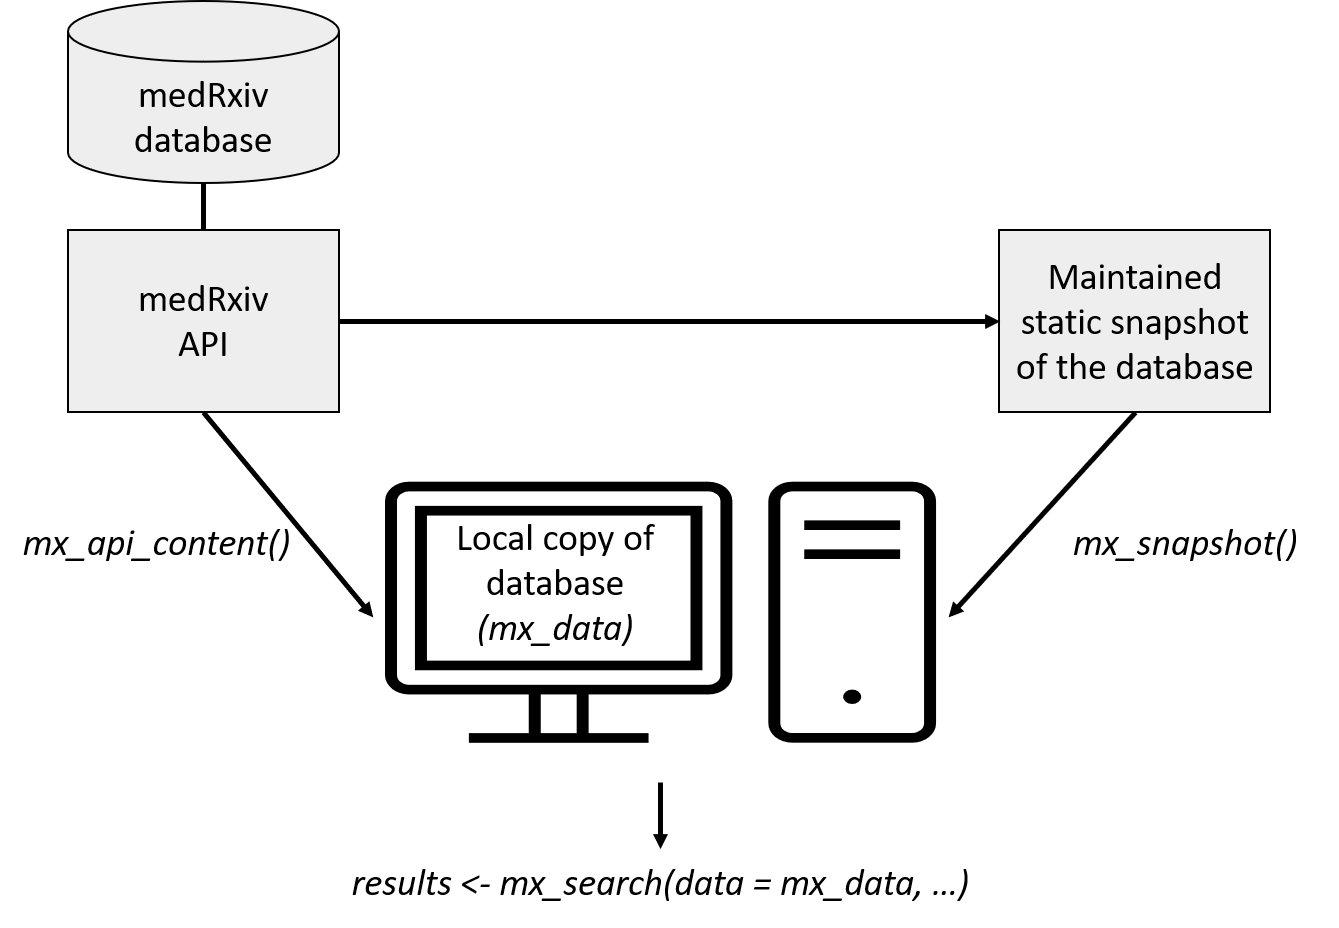
\includegraphics[width=1\linewidth]{figures/sys-rev-tools/data_sources} \caption[Overview of \texttt{medrxivr} data sources]{\textbf{Overview of \texttt{medrxivr} data sources} - Users can either access the API directly via \texttt{mx\_api\_content()}, or can import a maintained snapshot of the database, taken each morning at 6am, via the \texttt{mx\_snapshot()} function. Note: due to the size of bioRxiv, only a maintained snapshot of the medRxiv repository is available via \texttt{mx\_snapshot()}.}\label{fig:medrxivr-data-sources}
\end{figure}

~

~

\hypertarget{performing-a-search}{%
\subsection{Performing a search}\label{performing-a-search}}

Once a local copy of the metadata is created, the first step in searching it is to create a search strategy. Search terms to be combined with the OR operator are contained in vectors (\texttt{c(...)}), while topics to be combined with the AND operator are contained in lists (\texttt{list(...)}).

~

\begin{Shaded}
\begin{Highlighting}[]
\CommentTok{\# Create the search query}
\NormalTok{topic1  }\OtherTok{\textless{}{-}} \FunctionTok{c}\NormalTok{(}\StringTok{"dementia"}\NormalTok{,}\StringTok{"alzheimer\textquotesingle{}s"}\NormalTok{)  }\CommentTok{\# Combined with OR}
\NormalTok{topic2  }\OtherTok{\textless{}{-}} \FunctionTok{c}\NormalTok{(}\StringTok{"lipids"}\NormalTok{,}\StringTok{"statins"}\NormalTok{)        }\CommentTok{\# Combined with OR}

\NormalTok{myquery }\OtherTok{\textless{}{-}} \FunctionTok{list}\NormalTok{(topic1, topic2)         }\CommentTok{\# Combined with AND}
\end{Highlighting}
\end{Shaded}

~

For example, when written in standard syntax, the search contained in the \texttt{myquery} object above would be: ``((dementia \textbf{OR} alzheimer's) \textbf{AND} (lipids \textbf{OR} statins))''. There is no limit to the number of search terms that can be included in each topic, nor in the number of topics that can be search for. Search terms can also contain common syntax used by systematic reviewers and health librarians, including the use of NEAR statements which allows for identification of co-localised terms, and wild-cards, which allow for alternate spellings, e.g.~``randomi\emph{s}ation'' vs ``randomi\emph{z}ation''.

Once a strategy has been defined, it is passed along with the local copy of the database to the \texttt{mx\_search()} function.

~

\begin{Shaded}
\begin{Highlighting}[]
\CommentTok{\# Run the search}
\NormalTok{results }\OtherTok{\textless{}{-}} \FunctionTok{mx\_search}\NormalTok{(mx\_data,}
\NormalTok{                     myquery)}
\end{Highlighting}
\end{Shaded}

~

\hypertarget{refining-a-search}{%
\subsection{Refining a search}\label{refining-a-search}}

An important argument of the \texttt{mx\_search()} is \texttt{report}, which outputs a structured table with each search strategy presented on an individual line and the number of records associated with this strategy.\textsuperscript{\protect\hyperlink{ref-rethlefsen2021prisma}{126}}

~

\begin{Shaded}
\begin{Highlighting}[]
\NormalTok{results  }\OtherTok{\textless{}{-}} \FunctionTok{mx\_search}\NormalTok{(mx\_data,}
\NormalTok{                      myquery,}
                      \AttributeTok{report =} \ConstantTok{TRUE}\NormalTok{)}
\end{Highlighting}
\end{Shaded}

\begin{Shaded}
\begin{Highlighting}[]
\DocumentationTok{\#\# Found 1 record(s) matching your search.}
\DocumentationTok{\#\# }
\DocumentationTok{\#\# Total topic 1 records: 224}
\DocumentationTok{\#\# dementia: 224}
\DocumentationTok{\#\# alzheimer\textquotesingle{}s: 0}
\DocumentationTok{\#\# }
\DocumentationTok{\#\# Total topic 2 records: 119}
\DocumentationTok{\#\# lipids: 90}
\DocumentationTok{\#\# statins: 33}
\end{Highlighting}
\end{Shaded}

~

This allows users to discover which terms in their search are contributing most to the total number of results returned. This is important as part of developing a search strategy,\textsuperscript{\protect\hyperlink{ref-bramer2018}{115}} as it allows for the key terms related to each topic to be discovered. It also aids in identifying misspelled or case-sensitive search terms, which will frequently return no results. As an example, in the search presented above, the term ``alzheimer's'' returns no records. This is expected, as ``Alzheimer'' is a proper noun and so should be capitalised, but serves to illustrate the usefulness of the reporting function.

~

\hypertarget{exporting-to-a-bibliography-file}{%
\subsection{Exporting to a bibliography file}\label{exporting-to-a-bibliography-file}}

In line with my second success criteria (Section \ref{success-criteria}), one of the key features of the \texttt{medrxivr} is the ability for users to easily export the results of their systematic search to a reference manager. While it is a seemingly simple request, this is is one of the key ways in which \texttt{medrxivr} is set apart for other preprint search tools, including the native medRxiv/bioRxiv website search functionality.

For example, the results of our simple search above can be exported to the \texttt{"medrxiv\_export.bib"} file using the following code:

~

\begin{Shaded}
\begin{Highlighting}[]
\FunctionTok{mx\_export}\NormalTok{(results, }
          \AttributeTok{file =} \StringTok{"medrxiv\_export.bib"}\NormalTok{,}
          \AttributeTok{report =} \ConstantTok{TRUE}\NormalTok{)}
\end{Highlighting}
\end{Shaded}

~

\hypertarget{downloading-the-pdfs-of-relevant-records}{%
\subsection{Downloading the PDFs of relevant records}\label{downloading-the-pdfs-of-relevant-records}}

\texttt{medrxivr} alos allows users to download the full text papers for records that are deemed eligible for full-text screening (see Figure \ref{fig:medrxivr-sr}). \texttt{mx\_download()} takes the list of included records and saves the PDF for each to a folder specified by the user. This functionality is similar to the ``Find Full Text'' feature offered by EndNote.

~

\begin{Shaded}
\begin{Highlighting}[]
\FunctionTok{mx\_download}\NormalTok{(results,  }\CommentTok{\# Search results, less excluded records}
            \StringTok{"pdf/"}\NormalTok{)   }\CommentTok{\# Directory to save PDFs to }
\end{Highlighting}
\end{Shaded}

~

\hypertarget{discussion}{%
\section{Discussion}\label{discussion}}

\hypertarget{reception-and-future-plans}{%
\subsection{Reception and future plans}\label{reception-and-future-plans}}

The tool has been well received by the community (as of December 2021, \texttt{medrxivr} has been downloaded more than 6100 times), and several use cases have been reported. It has been used to investigate the role of preprints in the response to the 2019 coronavirus outbreak,\textsuperscript{\protect\hyperlink{ref-kodvanj2020}{127}} perform searches of preprints as part of a systematic review,\textsuperscript{\protect\hyperlink{ref-noone2020}{128},\protect\hyperlink{ref-grassly2020}{129}} and examine how data-sharing behaviour is affected by journal policies (see \ref{thesis-output}).\textsuperscript{\protect\hyperlink{ref-mcguinness2020DAScomparison}{130}}

The package has been accepted into the rOpenSci suite of packages, a collection of ``carefully vetted, staff- and community-contributed R software tools that lower barriers to working with scientific data sources on the web''.\textsuperscript{\protect\hyperlink{ref-boettiger2015}{131}} As part of this process, following rigorous peer-review, an associated article introducing the tool was published by the Journal of Open Source Software.\textsuperscript{\protect\hyperlink{ref-mcguinness2020medrxivr}{132}} The entire review discussion is publicly available and can be viewed online.\textsuperscript{\protect\hyperlink{ref-zotero-15016}{133}} The tool has also been well received by the open-source community, demonstrated by the engagement of other developers in contributing to important new functionality and suggesting bug-fixes.

Lobbying of the Cold Springs Harbor Laboratory to develop the API to allow for direct searching of the database has been ongoing. This would negate the current need to download a local copy of the relevant preprint database before searching it, which is currently the rate limiting step for performing searches. For example, as of January 2021, downloading a copy of the bioRxiv database takes approximately an hour.

~

\hypertarget{use-cases}{%
\subsection{Use cases}\label{use-cases}}

In addition to being used to search systematically search health-related preprint servers, as illustrated in the systematic review presented in Chapter \ref{sys-rev-heading}, \texttt{medrxivr} has other uses.

For example, I led a descriptive analysis of the change in data availability statements between preprinted and published versions of the same manuscript, stratified by journal data sharing policy access, underpinned by preprint meta-data provided by \texttt{medrixvr}. By comparing the preprinted and published versions of the data availability statement, I could examine the same manuscript (same content, authors and funders) under two different publication policies, and examine whether stricter policies which require data sharing as a condition of publication actually result in increased data availability. We found some evidence that data availability statements more frequently described open data on publication when the journal mandated data sharing compared to when the journal did not mandate data sharing. This study has since been published in PLOS One, and a copy is included in Appendix \ref{published-papers}.

Secondly, using \texttt{medrxivr}, an analysis of the publication rate for medRxiv preprints was performed (see Appendix \ref{appendix-sys-rev-tools}). Eighty-seven (67.4\%) of the 129 records posted on medRxiv in July 2019 were published by 30th July 2021 (i.e.~allowing for a two-year lag between preprint posting and publication). This finding agrees with previous work demonstrating that two-thirds of bioRxiv preprints are published in a peer-reviewed journal within two years of posting,\textsuperscript{\protect\hyperlink{ref-abdill2019popularity}{134}} indicating that a non-insignificant number of preprints are never formally published but remain accessible as preprints.

In short, these use cases illustrate that easy access to medRxiv/bioRxiv metadata has applications beyond systematic searching of preprints by enabling meta-research/methodological analyses.

\hypertarget{medrxivr-limitations}{%
\subsection{\texorpdfstring{Limitations of \texttt{medrxivr}}{Limitations of medrxivr}}\label{medrxivr-limitations}}

While searching of the medRxiv and bioRxiv databases was crucial for the systematic review element of my thesis presented in Chapter \ref{sys-rev-heading}, there are some important limitations to note here. A key example is that the tool only searches the available metadata of preprint records (the title, abstract and keywords), rather than the full text of preprints, meaning some relevant records might be missed. However, this approach echoes that used by other search platforms such as OvidSP, and while some relevant records may be missed (reduced sensitivity), limiting the search to the metadata fields prevents non-relevant records from being returned (high specificity). A key example of the reduced specificity when searching the full text, identified during development of \texttt{medrxivr}, is that a search for ``dementia'' would return a record where the only occurrence of this term is in the title of one of the references.\textsuperscript{\protect\hyperlink{ref-bong2019}{135}}

There is also the potential that the cross-section of literature posted on medrxiv/bioRxiv is substantially different those suffering from publication bias (studies or analyses that are not published for a range of reasons including results that are not deemed ``novel'' or are not statistically significant).\textsuperscript{\protect\hyperlink{ref-song2010}{136}} This is because simply lowering the barriers to publication may well encourage authors to published ``null'' results, but due to the effort involved in writing up a distributable manuscript, it is unlikely to completely address the ``file drawer'' effect.\textsuperscript{\protect\hyperlink{ref-rosenthal1979}{83}}

It is likely too early (and likely too methodologically difficult) to tell whether the increased popularity and acceptance of preprint repositories will have any effect of the availability of research that was not considered ``publishable'' at other venues.

~

\hypertarget{role-of-open-source-tools-in-evidence-synthesis}{%
\subsection{Role of open source tools in evidence synthesis}\label{role-of-open-source-tools-in-evidence-synthesis}}

Part of the motivation for creating the \texttt{medrxivr} tool was a belief that the development and distribution of open source scripts and tools should be a fundamental part of evidence synthesis research.\textsuperscript{\protect\hyperlink{ref-goldacre2019}{137},\protect\hyperlink{ref-mckiernan2016}{138}} In the case of \texttt{medrxivr}, it is likely that several other evidence synthesists had written personal scripts that have a similar, or related, functionality - in fact, following development of the tool, I identified one other researcher that has done so (Nicholas Fraser, author of the \texttt{rbiorxiv} package, which allows for importing medRxiv metadata into R but does not provide search functionality).\textsuperscript{\protect\hyperlink{ref-fraser2020rbiorixv}{139}} If these scripts continue to be developed in private and are never shared or publicised, this will inevitably hamper the efforts of evidence synthesis community, not only in terms of duplication of time and effort but also due to lost opportunities for collaboration.\textsuperscript{\protect\hyperlink{ref-mckiernan2016}{138}} Creating and sharing well-documented packages, the recognised standard for sharing code in R, represents one way to reduce this inefficiency.\textsuperscript{\protect\hyperlink{ref-vuorre2020}{140}}

\hypertarget{summary-1}{%
\section{Summary}\label{summary-1}}

\begin{itemize}
\item
  In this Chapter, I have introduced a new tool, \texttt{medrxivr}, for performing complex systematic searches of the medRxiv and bioRxiv preprint repositories.
\item
  I have outlined the motivation for developing this tool in relation to this thesis - more specifically, that it was used to perform systematic and reproducible searches of a key literature sources used in the comprehensive systematic review described in Chapter \ref{sys-rev-heading}.
\item
  I have contrasted \texttt{medrxivr} with other available interfaces to medRxiv/bioRxiv data to highlight the added functionality it offers. I have also discussed the tools reception to date, its limitations, and the important role of open-source tools like \texttt{medrxivr} in evidence synthesis.
\end{itemize}

\newpage

\hypertarget{references-1}{%
\section{References}\label{references-1}}

\begin{savequote}
``It is surely a great criticism of our profession that we have not
organised a critical summary by speciality or sub-speciality, up-dated
periodically, of all relevant RCTS.''
\qauthor{--- Archibald Cochrane, 2000\textsuperscript{\protect\hyperlink{ref-cochrane1979}{141}}}\end{savequote}



\hypertarget{sys-rev-methods-heading}{%
\chapter{Systematic review of existing evidence on the association between blood lipids and dementia outcomes: Methods}\label{sys-rev-methods-heading}}

\minitoc 

\hypertarget{lay-summary-2}{%
\section{Lay summary}\label{lay-summary-2}}

Systematic reviews are a type of research study that aim to collect and combine all existing evidence to provide the best possible answer to an important research question. Well-performed reviews involve multiple steps including: searching of existing studies; assessment of the studies against predefined inclusion criteria; collection of data from each study; and assessment of each study's method and results.

This chapter presents the methods used to perform a systematic review of primary studies that have examined the relationship between the levels of blood lipids (such as cholesterol and triglycerides) and dementia outcomes. In addition, the review examined the relationship between treatments that change blood lipid levels, such as statins, and dementia outcomes. The results of this systematic review are then presented in Chapter @ref(sys-rev-results-heading.)

~

\hypertarget{sys-rev-intro}{%
\section{Introduction}\label{sys-rev-intro}}

In this chapter, I describe a comprehensive systematic review of the relationship between blood lipid levels (and treatments that modify them) and the subsequent risk of dementia and related outcomes.

This analysis sought to address two specific aims. Firstly, as discussed in the introduction to this thesis (Section \ref{evidence-association}), several diverse forms of evidence on the relationship of lipids and dementia exist. These include randomised controlled trials, observational studies of different design, and Mendelian randomisation studies. However, based on a scoping review of existing literature, no previous evidence synthesis exercise has attempted to examine the association of lipids/statins with dementia outcomes across these distinct evidence types. Collating these diverse evidence sources is important, as if the observed association between lipids and dementia is constant across them, it increases our confidence in the association. As such, the primary aim of this analysis was to systematically review all available literature describing prospective analyses, regardless of study design.

Secondly, I explicitly sought to include health-related preprint servers as a potential evidence source in this review, as they are infrequently considered by evidence synthesists but report relevant unpublished analyses. As a sensitivity analysis to this review presented in this chapter, I sought to quantify the additional evidential value of including preprints, making use of the preprint search tool presented in Chapter \ref{sys-rev-tools-heading}.

Given the size of the review, I have seperated the methods and results into two chapters for ease of reading. This chapter details the methodology used, while CHapter \ref{sys-rev-results-heading} presents the results of the review.

~

\hypertarget{methods}{%
\section{Methods}\label{methods}}

\hypertarget{protocol}{%
\subsection{Protocol}\label{protocol}}

A pre-specified protocol for this analysis was registered on the Open Science Framework platform and is available for inspection.\textsuperscript{\protect\hyperlink{ref-mcguinnessluke2020}{142}}

~

\hypertarget{contributions}{%
\subsection{Contributions}\label{contributions}}

In line with best-practice guidance, secondary reviewers were used to check the accuracy of screening, data extraction and risk-of-bias assessment processes. Due to the scale of the project, this review was performed in conjunction with a team of secondary reviewers (see Acknowledgements and Author Declaration in the front matter).

~

\hypertarget{eligibility-criteria}{%
\subsection{Eligibility criteria}\label{eligibility-criteria}}

\hypertarget{inclusion-criteria}{%
\subsubsection{Inclusion criteria}\label{inclusion-criteria}}

I sought to include studies that examined blood lipid levels as a risk factor for dementia outcomes, defined either as binary hypercholesterolemia variable or by category/1-standard-deviation increase of a specific lipid fraction (total cholesterol, high- and low-density lipoprotein cholesterol and triglycerides). I also aimed to include studies examining the effect of treatments that modify blood lipid levels, such as statins or fibrates, as a source of indirect evidence.

Eligible study designs were randomized controlled trials, non-randomized studies of exposures, non-randomised studies of , longitudinal studies examining the effect of increased/decreased blood lipid levels, and genetic instrumental variable (Mendelian randomization) studies examining the effect of genetically increased/decreased blood lipid levels.

Eligible studies screened participants for dementia at baseline and excluded any prevalent cases. Alternatively, where no baseline screening was employed, participants were assumed to be dementia free if less than 50 years of age at baseline. Studies of any duration were included to allow for exploration of the effect of length of follow-up on the effect estimate using meta-regression. No limits were placed on the sample size of included studies.

Eligible studies defined dementia outcomes according to recognised criteria, for example the International Classification of Diseases (ICD),\textsuperscript{\protect\hyperlink{ref-organizationwho1993}{143}} National Institute of Neurological Disorders and Stroke Association-Internationale pour la Recherche en l'Enseignement en Neurosciences (NINDS-AIREN),\textsuperscript{\protect\hyperlink{ref-roman1993}{13}} or Diagnostic and Statistical Manual of Mental Disorders (DSM) criteria.\textsuperscript{\protect\hyperlink{ref-edition2013}{3}} Studies utilising electronic health records were the exception to this, as it was assumed that a valid criteria was employed when entering used when entering the outcome into the EHR.

Conference abstracts with no corresponding full-text publication were eligible, and where required, I contacted authors to obtain information on the study's status. No limitations were imposed on publication status, date, venue or language.

~

\hypertarget{exclusion-criteria}{%
\subsubsection{Exclusion criteria}\label{exclusion-criteria}}

Due to the significant impact of a memory-related outcome such as dementia on exposure recall, case-control studies were excluded, though case-control studies where historical records are used to determine the exposure status, were eligible for inclusion. Cross-sectional studies, qualitative studies, case reports/series and narrative reviews were also excluded, as were studies that measure change in continuous cognitive measures (e.g.~MoCA score) without an attempt to map these scores to ordinal groups (e.g.~no dementia/dementia). Previous systematic reviews were not eligible for inclusion, but their reference lists were screened to identify any potentially relevant articles.

Studies with outcomes not directly related to the clinical syndrome of dementia (e.g., neuroimaging), studies implementing a ``multi-domain intervention'' where a lipid-regulating agent is included in each arms (e.g.~for example, a study examining exercise + statins vs statins alone, but a study examining exercise + statins vs exercise alone would be included), and studies where there was no screening for dementia at baseline except if the sample was initially assessed in mid-life (i.e.~below the age of 50) were excluded. Finally, studies using a dietary intervention, for example omega-3 fatty acid enriched diet, were excluded as it is difficult to disentangle the effect of other elements contained within the diet. Note, this is distinct from studies which delivered a simple tablet-based omega-3 intervention, which would have been eligible for inclusion.

~

\hypertarget{information-sources-and-search-strategy}{%
\subsection{Information sources and search strategy}\label{information-sources-and-search-strategy}}

I systematically searched several electronic bibliographic databases to identify potentially relevant entries (hereafter referred to as ``records''). The following databases were searched from inception onwards: Medline, EMBASE, Psychinfo, Cochrane Central Register of Controlled Trials (CENTRAL), and Web of Science Core Collection. As the contents of the Web of Science Core Collection can vary by institution,\textsuperscript{\protect\hyperlink{ref-gusenbauer2020}{116}} the specific databases and date ranges for each database searched via this platform are listed in Appendix \ref{appendix-wos-databases}. The search strategy used in each database was developed in an iterative manner using a combination of free text and controlled vocabulary (MeSH/EMTREE)\textsuperscript{\protect\hyperlink{ref-lefebvre2019searching}{79}} terms to identify studies which have examined the relationship between blood lipids levels and dementia, incorporating input from an information specialist. The strategy included terms related to lipids, lipid modifying treatments, and dementia, and was designed for MEDLINE before being adapted for use in the other bibliography databases listed. A high-level outline of the strategy is presented in the Table \ref{tab:searchOverview-table} below and the full search strategies for each database are presented in Appendix \ref{appendix-search-strategy}.

~





\begin{table}[H]

\caption[searchOverview]{\label{tab:searchOverview-table}Summary of systematic search by topic. The full search strategy including all terms and the number of hits per term is included in Appendix \ref{appendix-search-strategy}.}
\centering
\fontsize{10}{12}\selectfont
\begin{threeparttable}
\begin{tabular}[t]{>{}cl}
\toprule
\textbf{No.} & \textbf{Concept}\\
\midrule
1 & Dementia\\
\midrule
2 & Lipids\\
\midrule
3 & Lipid-modifying treatments\\
\midrule
4 & 1 AND 2\\
\midrule
5 & 1 AND 3\\
\midrule
\addlinespace
6 & 4 OR 5\\
\midrule
7 & Animals NOT (Animals AND Humans)\\
\midrule
8 & 6 NOT 7\\
\midrule
9 & Observational filter\\
\midrule
10 & Randomised controlled trial (RCT) filter\\
\midrule
\addlinespace
11 & Mendelian randomisation/Instrumental variable filter\\
\midrule
12 & OR/ 9-11\\
\midrule
13 & 8 AND 12\\
\bottomrule
\end{tabular}
\begin{tablenotes}
\item For all topics, search queries were comprised of relevant free text \& controlled vocabulary terms.
\end{tablenotes}
\end{threeparttable}
\end{table}

~

When searching the bibliographic databases, study design filters were employed to try and reduce the screening load. To ensure that the study design filters were not excluding potentially relevant records, a random sample of 500 records identified by the main search but excluded by the filters (defined as ``8 NOT 12'' in Table \ref{tab:searchOverview-table}) was screened.

I also searched clinical trial registries, for example ClinicalTrials.gov, to identify relevant randomized controlled trials. In addition, I searched the bioRxiv and medRxiv preprint repositories using the tool developed in Chapter \ref{sys-rev-tools-heading} to identify potentially relevant preprinted studies (see Appendix \ref{appendix-medrxivr-code} for the code used to search these preprint repositories).

Grey literature was searched via ProQuest, OpenGrey and Web of Science Conference Proceedings Citation Index, while theses were accessed using the Open Access Theses and Dissertations portal. In addition, the abstracts list of relevant conferences (e.g.~the proceedings of the Alzheimer's Association International Conference, published in the journal Alzheimer's \& Dementia) were searched by hand. Finally, the reference lists of included studies were searched by hand while studies citing included studies was examined using Google Scholar (forward and reverse citation searching or ``snowballing''\textsuperscript{\protect\hyperlink{ref-greenhalgh2005}{144},\protect\hyperlink{ref-wohlin2014}{145}}).

~

\hypertarget{study-selection}{%
\subsection{Study selection}\label{study-selection}}

Records were imported into Endnote and de-duplicated using the method outlined in Bramer et al.~(2016).\textsuperscript{\protect\hyperlink{ref-bramer2016}{146}} In summary, this method uses multiple stages to identify potential duplicates, beginning with automatic deletion of records matching on multiple fields (``Author'' + ``Year'' + ``Title'' + ``Journal''), followed by manual review of less similar articles (e.g.~those identified as duplicates based on the ``Title'' field alone).

Following de-duplication of records, screening (both title/abstract and full-text) was performed using a combination of Endnote, a citation management tool,\textsuperscript{\protect\hyperlink{ref-hupe2019}{147}} and Rayyan, a web-based screening application.\textsuperscript{\protect\hyperlink{ref-ouzzani2016}{148}} Title and abstract screening to remove obviously irrelevant records was performed primarily by me, with a random \textasciitilde10\% sample of excluded records being screened in duplicate to ensure consistency with the inclusion criteria. Additionally, I re-screened the same \textasciitilde10\% sample with 3 month lag to assess intra-rater consistency.

Similarly, I completed all full-text screening, with a random \textasciitilde20\% being screened in duplicate by a second reviewer, in addition to any records identified I identified as being difficult to assess against the inclusion criteria were screened in duplicate. Reasons for exclusion at this stage were recorded. Disagreements occurring during either stage of the screening process were resolved through discussion with a senior colleague. A PRIMSA flow diagram was produced to document how records moved through the review.\textsuperscript{\protect\hyperlink{ref-page2021}{92}}

The criteria against which records were assessed for eligibility are presented above.

~

\hypertarget{validation-of-screening-process}{%
\subsection{Validation of screening process}\label{validation-of-screening-process}}

Inter- and intra-rater reliability during the screening stages were assessed for a 10\% sub-sample of records. Intra-rater reliability involved a single reviewer applying the inclusion criteria to the same set of records while blinded to their previous decisions (i.e.~assessment of consistency), while inter-rater reliability involved two reviewers independently screening the same set of records (i.e.~assessment of accuracy).

Rater reliability was assessed using Gwet's agreement coefficient (AC1).\textsuperscript{\protect\hyperlink{ref-gwet2008}{149}} This measure was chosen over other methods such as percent agreement (number of agreements divided by total number of assessments), as it accounts for chance agreement between reviewers but does not suffer from bias due to severely imbalanced marginal totals in the same way that Cohen's \(kappa\) value does.\textsuperscript{\protect\hyperlink{ref-gwet2008}{149}} Given the small number of included studies in this review as a proportion of the total number screened, this is a useful characteristic.

How to interpret agreement coefficients is widely debated, and while arbitrary cut-off values may mislead readers,\textsuperscript{\protect\hyperlink{ref-brennan1992}{152}} they provide a useful rubric by which to assess inter-rater agreement. Here, I used guidelines based on a stricter interpretation of the Cohen's \(kappa\) coefficient,\textsuperscript{\protect\hyperlink{ref-mchugh2012}{153}} presented in Table \ref{tab:gwet-table}.

~





\begin{table}[H]

\caption[Ranges for Gwet's AC1]{\label{tab:gwet-table}Suggested ranges to aid in interpretation of Gwet's AC1 inter-rater reliability metric}
\centering
\begin{tabular}[t]{cc}
\toprule
\textbf{Kappa} & \textbf{Interpretation}\\
\midrule
0    – 0.20 & None\\
\midrule
0.21 – 0.39 & Minimal\\
\midrule
0.40 – 0.59 & Weak\\
\midrule
0.60 – 0.79 & Moderate\\
\midrule
0.80 – 0.90 & Strong\\
\midrule
\addlinespace
> 0.90 & Almost perfect\\
\bottomrule
\end{tabular}
\end{table}

~

Intra- and inter-rater reliability was assessed against these cut-offs. If this assessment demonstrated issues with the screening process (defined as an AC1 of less than .9), a larger proportion of records would have been dual-screened.

~

\hypertarget{data-extraction}{%
\subsection{Data extraction}\label{data-extraction}}

Data extraction was performed using a piloted data extraction form. Extracted items included: article metadata (year of publication, author list, journal), study characteristics (study location, data source, exposure, outcomes, outcome criteria used), patient characteristics (age, sex, baseline cognition scores, baseline education scores), and results (exposure-outcome pairing, effect measure, effect estimate, error estimate, p-value). I extracted all data in the first instance, which was subsequently checked for accuracy by a second member of the review team.

~

\hypertarget{grouping-multiple-reports-into-studies}{%
\subsubsection{Grouping multiple reports into studies}\label{grouping-multiple-reports-into-studies}}

As part of the data extraction process, multiple records resulting from a single analysis were included and grouped into single units, hereafter called studies. This was most common in cases where multiple records reported on the same analysis but at different time points. In this case, the result corresponding to the longest follow-up was used. Grouping records into studies builds out the most comprehensive account of a given analysis by incorporating information from all available records.

This was particularly relevant to preprints and published papers reporting the same study, which were not considered to be duplicate records but instead different reports of the same study. This is due to the potential for the published version to offer some information that the preprint did not, and vice versa.

~

\hypertarget{combining-across-groups}{%
\subsubsection{Combining across groups}\label{combining-across-groups}}

In line with best practice, where summary data were presented across two groups (e.g.~age at baseline stratified by hypercholesterolemia status), the following approach was used to combine the groups:\textsuperscript{\protect\hyperlink{ref-higgins2019}{154}}

\begin{equation}
N = N_1 + N_2
  \label{eq:combiningGroups1}
\end{equation}

\begin{equation}
Mean = \frac{(N_1M_1 + N_2M_2)}{(N_1 + N_2)}
  \label{eq:combiningGroups2}
\end{equation}

\begin{equation}
SD = \sqrt{\frac{(N_1-1)SD_1^2 + (N_2-1)SD_2^2 + \frac{N_1N_2}{N_1 + N_2}(M_1^2 + M_2^2 - 2M_1M_2)}{N1 + N2 -1}}
  \label{eq:combiningGroups3}
\end{equation}

~

This was implemented in a systematic manner, with the raw group data being extracted and a cleaning script employed to combine the groups for analysis.

~

\hypertarget{harmonisation-of-cholesterol-measures}{%
\subsubsection{Harmonisation of cholesterol measures}\label{harmonisation-of-cholesterol-measures}}

Where necessary, lipid levels reported in \emph{mmol/L} were converted in \emph{mg/dL} using the following formula:

\begin{equation} 
  mg/dL = mmol/L \times{} Z
  \label{eq:lipidConversion}
\end{equation}

where \(Z = 38.67\) for total cholesterol, LDL-c and HDL-c, and \(Z = 88.57\) for triglycerides.\textsuperscript{\protect\hyperlink{ref-rugge2011}{155}} The choice of \emph{mg/dL} was influenced by the widely-used categorises of lipids levels on the \emph{mg/dL} scale, as shown in Table \ref{tab:lipidLevels-table} in Section \ref{intro-lipid-fractions}.

~

\hypertarget{contacting-authors}{%
\subsubsection{Following up with authors}\label{contacting-authors}}

Where additional data points not included in the report of an analysis were required either for the analysis or risk-of-bias assessment, the corresponding author of the study was contacted. This approach was taken due to the potentially large impact of following up with authors on the results of the review.\textsuperscript{\protect\hyperlink{ref-reynders2019}{156}}

~

\hypertarget{risk-of-bias}{%
\subsection{Risk-of-bias assessment}\label{risk-of-bias}}

A key aim of the review presented in this chapter is to identify different sources of evidence at risk of a diverse range of biases, and to contrast and compare findings across them (see Section \ref{triangulation-overview} for an overview of triangulation and Chapter \ref{tri-heading} for the results of this analysis). To enable this triangulation exercise, a detailed and structured risk-of-bias assessment formed an important part of this review.

There has been a recent movement within the evidence synthesis community away from examining \emph{methodological quality} to assessing \emph{risk of bias},\textsuperscript{\protect\hyperlink{ref-mcguinness2018}{94},\protect\hyperlink{ref-sterne2016}{157}} and thus directly evaluating the internal validity of a study. Internal validity is defined here as the absence of systematic error (or bias) in a study, which may influence its results.\textsuperscript{\protect\hyperlink{ref-campbell1957}{158},\protect\hyperlink{ref-juni2001}{159}}

This move was prompted by an unclear definition of ``methodological quality'' which could include facets such as unclear reporting, in addition to challenges in the comparison of results from different tools. As part of this shift, the focus shifted from checklist or score based tools towards domain-based methods, in which different potential sources of bias in a study are assessed in order.
Finally, the new tools tools move from assessing bias at the study level to considering separately each individual numerical result reported. For example, a study may report on the efficacy of an intervention at six months and two years follow-up. In this case, missing outcome data that are not an issue at six months may introduce bias after two years of follow-up, and assigning a single risk-of-bias judgement to the study as a whole masks the different biases applicable to each unique result.

In this review, domain-based tools were used to assess the risk of bias for each result in each included study. The study design-specific tools are introduced and discussed in more detail in the following sections.

~

\hypertarget{randomised-controlled-trials-1}{%
\subsubsection{Randomised controlled trials}\label{randomised-controlled-trials-1}}

Randomized controlled trials were assessed using the RoB 2 tool.\textsuperscript{\protect\hyperlink{ref-sterne2019}{93}} The tool assesses the risk of bias across five domains: bias arising from the randomization process, bias due to deviations from intended intervention, bias due to missing outcome data, bias in measurement of the outcome, bias in selection of the reported result. Acceptable judgements for each domain include: ``low risk'', ``some concerns'', ``high risk''. Each of the five domains contains a series of signaling questions or prompts which guide the user through the tool. Once a domain-level judgement for each domain has been assigned, an overall judgement, using the same three levels of risk of bias, is assigned to the result.

~

\hypertarget{rob-tools-nrse}{%
\subsubsection{Non-randomised studies of interventions/exposures}\label{rob-tools-nrse}}

For non-randomised studies of interventions (NRSI), I used the ROBINS-I (Risk Of Bias In Non-randomised Studies - of Interventions) tool.\textsuperscript{\protect\hyperlink{ref-sterne2016}{157}} This tool assess the risk of bias across seven domains: bias due to confounding, bias due to selection of participants, bias in classification of interventions, bias due to deviations from intended interventions, bias due to missing data, bias in measurement of outcomes, and bias in selection of the reported result. Similar to RoB 2, it has a number of prompting questions per domain, with acceptable judgements including ``low risk'', ``moderate risk'', ``serious risk'' and ``critical risk''. In the context of the tool, observational studies are assessed in reference to an idealised randomised controlled trial. Under this approach, the (rare) overall judgement of ``Low'' indicates that the results should be considered equivalent to that produced by a randomised controlled trial.

While a risk-of-bias tool for non-randomised studies of exposures (NRSE) is currently under development,\textsuperscript{\protect\hyperlink{ref-morganr2020}{160}} but was insufficiently developed at the time the risk-of-bias assessments for this review were performed. Instead, I used a version of the ROBINS-I tool informed by the preliminary ROBINS-E tool (Risk of Bias In Non-randomised Studies -- of Exposure), which I had previously applied in a published review.\textsuperscript{\protect\hyperlink{ref-french2019}{161}} The version had no signaling questions and so judgements, using the same four levels of bias as ROBINS-I, were made at the domain level. The motivation using this tool above other established tools such as the Newcastle-Ottowa scale (NOS)\textsuperscript{\protect\hyperlink{ref-wells2000}{162}} was two-fold. In the first instance, as mentioned in the introduction to this section, using a domain-based tool has distinct advantages over better-developed checklist-type tools including the NOS. Additionally, using a domain-based tool for non-randomised studies of exposures enabled better comparison with risk-of-bias assessments performed for the other study designs as part of this review.

~

\hypertarget{mendelian-randomisation-studies}{%
\subsubsection{Mendelian randomisation studies}\label{mendelian-randomisation-studies}}

At present, no formalised risk-of-bias assessment tool for Mendelian randomization studies is available. Assessment of the risk of bias in Mendelian randomisation studies was informed by the approach used in a previous systematic review of Mendelian randomisation,\textsuperscript{\protect\hyperlink{ref-mamluk2020}{163}} as identified by a review of risk-of-bias assessments in systematic reviews of Mendelian randomisation studies (advance results from this review were obtained from contact with the review authors).\textsuperscript{\protect\hyperlink{ref-spiga2021}{164}} A copy of this tool is available in Appendix \ref{appendix-mr-rob}, but in summary, results were assessed for bias arising from weak instruments, genetic and other confounding, pleiotropy and population stratification. Acceptable judgements for each of the 5 domains in the tool included ``low'', ``moderate'' and ``high'' risk of bias.

~

\hypertarget{methods-rob-me}{%
\subsubsection{Risk of bias due to missing evidence}\label{methods-rob-me}}

In addition to assessing the risk of bias within each result contributing to a synthesis, I also assessed risk of bias due to missing evidence at the analysis level. This assessment examines evidence missing due to selective non-reporting - as distinct from the selective reporting of a single result from multiple planned analyses - and was performed using the forthcoming RoB-ME (Risk of Bias due to Missing Evidence in a synthesis) tool.\textsuperscript{\protect\hyperlink{ref-zotero-15123}{165}} The tool is in development stages, and as part of this review, I piloted the tool, and provided feedback to the developers.

This additional appraisal marks a departure from the registered protocol, as there was initially no intention to try and examine the risk of bias due to missing evidence. This is largely because the tool did not exist when the protocol was registered.

~

\hypertarget{analysis-methods}{%
\subsection{Analysis methods}\label{analysis-methods}}

An initial qualitative synthesis of evidence was performed, summarising the data extracted from studies stratified by study design. Where individual studies were deemed comparable, they were incorporated into a quantitative analysis or ``meta-analysis''.

~

\hypertarget{analysis-overview}{%
\subsubsection{Analysis overview}\label{analysis-overview}}

Results were not combined across different study designs (i.e.~RCTs were not combined in a meta-analysis with results from observational studies). The summary effect estimates produced across individual study designs are discussed, but are compared and contrasted more fully as part of the triangulation exercise presented in Chapter \ref{discussion-heading}. Analysis are presented seperately for each dementia type of interest.

The range of effect measures presented by studies (odds ratios, risk ratios, hazard ratios, etc) are not directly interchangeable in the context of systematic review. As such, different reported effect estimates can be one potential problem that precludes a meta-analysis of all studies.\textsuperscript{\protect\hyperlink{ref-mckenzie2019}{166}} However if the outcome is rare, as is the case for dementia outcomes, the estimated odds, risk and hazard ratios will approximate each other.\textsuperscript{\protect\hyperlink{ref-vanderweele2020}{167}} As such, I did not stratify the analyses by reported effect measure.

\hypertarget{random-effects-meta-analysis}{%
\subsubsection{Random-effects meta-analysis}\label{random-effects-meta-analysis}}

I used a random-effects model in all meta-analysis presented in this chapter.{[}\textsuperscript{\protect\hyperlink{ref-hedges1998}{168},\protect\hyperlink{ref-dersimonian1986}{169}} Random-effects meta-analysis does not assume one true underlying effect, but rather allows for a distribution of true effects with variance \(\tau^2\). The weight (\(w\)) assigned to each result (denoted as \(y_i\)) is then given as the inverse of variance of that result plus the estimate of between-result variance, denoted as \(w_i = \frac{1}{v_i+\tau^2}\) for result \(i\).

Once the weights are calculated for each result, the overall estimate (\(\hat{y}\)) and variance (\(Var(\hat{y})\)) can be estimated:

\begin{equation}
\hat{y} = \frac{\sum{y_iw_i}}{\sum{w_i}}
  \label{eq:rmaEstimate}
\end{equation}

\begin{equation}
Var(\hat{y}) = \frac{1}{\sum{w_i}}
  \label{eq:rmaVariance}
\end{equation}

~

Results were stratified into subgroups on the basis of the overall risk of bias assessment, and summary estimates for each subgroup, in addition to an overall effect estimate, are displayed in each forest plot. Additional descriptive statistics are presented, while prediction intervals are shown as a dotted line banding the overall effect estimate. Finally, where at least 10 results are available, a test of subgroup differences between studies at different levels of risk of bias was performed (see subsequent Section \ref{sys-rev-visualising-results}).\textsuperscript{\protect\hyperlink{ref-deeks2019}{170}} All models were implemented using the \texttt{metafor} R package.

~

\hypertarget{dose-response-analyses}{%
\subsubsection{Dose-response analyses}\label{dose-response-analyses}}

Several of the included studies presented data on multiple categories of lipid levels, but provided an overall effect estimate based on a comparison of only two of these categories (e.g.~for example, highest vs lowest quartile). While this allows for easy interpretation of the resulting effect estimate, it ignores any potential non-linear relationships between the exposure and outcome, in addition to discarding useful information contained in the interim groups. In order to address this limitation, I performed a dose-response meta-analysis in those studies reporting more than two categories for lipid levels. This marks a departure from the published protocol, as I was unaware that such a large number of studies would report dementia risk across multiple lipid categories.

Studies were excluded from this analysis if the number of categories was less than three or if the necessary information for synthesis (cut-off points, number of participants and number of events per category) was not available. When the highest reported category was open ended (e.g LDL-c \(\geqslant\) 200 mg/dL), I calculated the category midpoint by assuming the width of the highest category was the same as the one immediately below it. Similarly, when the lowest category was open-ended (e.g LDL-c \(\leqslant\) 100 mg/dL), I set the lower boundary for this category to zero (though this is unlikely to occur naturally).

I took a two-stage dose-response meta-analysis approach, where study-specific trends are estimated before being pooled acrosss studies.\textsuperscript{\protect\hyperlink{ref-greenland1992}{171}} To estimate within-study trends, a restricted cubic spline model was fitted within each to allow for a non-linear relationship between lipid levels and dementia, for example a U or J-shaped relationship, where low and high levels of a lipid fraction can have different effects versus the ``normal'' reference dose.\textsuperscript{\protect\hyperlink{ref-durrleman1989}{172},\protect\hyperlink{ref-liu2009}{173}}
Reference doses were defined \emph{a priori} as the cut-off of the ``Normal''/``Optimal'' categories for each fraction, as detailed in Table \ref{tab:lipidLevels-table}. Under this approach, the reference dose was defined as 200 mg/dL for total cholesterol, 100 mg/dL for LDL-c, 40 mg/dL for HDL-c, and 150 mg/dL for triglycerides.

Restricted cubic spline models use ``knots'' to create separate the data into subsets or ``windows'', in which the trend is modelled. Further restrictions are then imposed, in that the curves in each window must join up ``smoothly'' at the knot location, and that the trend is assumed to be linear before the first knot and after the last knot.\textsuperscript{\protect\hyperlink{ref-gauthier2020}{174}} The locations of the knots in the model were identified using fixed percentiles (5th, 50th, 95th) of the exposure data.\textsuperscript{\protect\hyperlink{ref-durrleman1989}{172}} Once the within-study trends have been estimated, they are combined in a multivariate random-effects meta-analysis using the restricted maximum likelihood method.\textsuperscript{\protect\hyperlink{ref-liu2009}{173},\protect\hyperlink{ref-white2009}{175},\protect\hyperlink{ref-gasparrini2012}{176}} All dose-response analyses were implemented using the \texttt{dosresmeta} R package.\textsuperscript{\protect\hyperlink{ref-crippa2016}{177}}

~

\hypertarget{additional-analyses}{%
\subsubsection{Additional analyses}\label{additional-analyses}}

Where there was evidence of heterogeneity between results included in a meta-analysis, I investigated this further using meta-regression against reported characteristics. \emph{A priori}, I was interested in the effect that the age at baseline, sex and risk-of-bias judgement had on the results. Syntheses with greater than 10 results were assessed for heterogeneity across these covariates.\textsuperscript{\protect\hyperlink{ref-deeks2019}{170}}

Finally, I investigated the potential for small study effects, which may be caused by publication bias, both visually using funnel plots and formally using Egger's regression test.\textsuperscript{\protect\hyperlink{ref-sterne2011}{178}}

~

\hypertarget{sys-rev-visualising-results}{%
\subsubsection{Visualisation of results}\label{sys-rev-visualising-results}}

Evidence maps are useful way to explore the distribution of research cohorts included in a systematic review.\textsuperscript{\protect\hyperlink{ref-saran2018}{179}} As part of the initial descriptive synthesis, the location of each individual study contributing to the evidence base was visualised on a world map.

One of the limitations of current risk-of-bias assessment practice in systematic reviews is that they are often divorced from the results to which they refer, and are infrequently incorporated into the analysis.\textsuperscript{\protect\hyperlink{ref-marusic2020}{180},\protect\hyperlink{ref-katikireddi2015}{181}} In response to this criticism, I developed a new visualisation tool which was designed to allow for the production of ``paired'' forest plots - a risk-of-bias assessment is presented alongside it's corresponding numerical result - as recommended by the ROB2 publication.\textsuperscript{\protect\hyperlink{ref-sterne2019}{93}} This tool was developed as an adjunct to this thesis to aid in creating standardised risk-of-bias figures,\textsuperscript{\protect\hyperlink{ref-mcguinness2020robvisPaper}{182}} and the ``paired'' forest plot functionality grew out of a collaboration with other researchers to design a modular method for creating custom forest plots.\textsuperscript{\protect\hyperlink{ref-zotero-14999}{183}} A summary of this tool is contained in Appendix \ref{appendix-robvis}, and all forest plots presented in this Chapter were created using this tool.

~

\hypertarget{assessment-of-added-value-of-including-preprints}{%
\subsubsection{Assessment of added value of including preprints}\label{assessment-of-added-value-of-including-preprints}}

Preprints are considered a valuable evidence source within this thesis (see Introduction, Section \ref{diverse-sources-preprints}). As an adjunct analysis to this review, I explored the additional evidential value of including preprints in each meta-analysis performed, assessed using the fixed effect weight from a standard meta-analysis. In addition, in meta-analysis including at least one preprinted result, I assessed the impact of including the preprinted results on the summary estimate using a leave-one-out approach.

Additionally, I followed identified preprints up after a two-year lag to investigate whether they had been subsequently published (in which case preprints provide a snapshot into the future, and a systematic review update would capture these reports) or not (in which case preprints provide a distinct evidence source to conventional bibliographic databases).

~

\hypertarget{summary-2}{%
\section{Summary}\label{summary-2}}

\begin{itemize}
\item
  In this chapter, I have presented the methods underpinning a comprehensive systematic review of the existing literature on the association of dementia incidence with blood lipids and treatments for lowering blood lipids.
\item
  I have highlighted how this review will make use of preprinted literature, using the research tool introduced in the preceding chapter (Chapter \ref(sys-rev-tools-heading)).
\item
  In the following chapter, I presented the results of this comprehensive systematic review and detail how the identified evidence is used throughout the remainder of the thesis.
\end{itemize}

\newpage

\hypertarget{references-2}{%
\section{References}\label{references-2}}

\begin{savequote}
Hold
\qauthor{--- Hold}\end{savequote}



\hypertarget{sys-rev-results-heading}{%
\chapter{Systematic review of existing evidence on the association between blood lipids and dementia outcomes: Results}\label{sys-rev-results-heading}}

\minitoc 

\hypertarget{lay-summary-3}{%
\section{Lay summary}\label{lay-summary-3}}

Using the methods outlined in the previous chapter, this chapter presents a systematic review of primary studies that have examined the relationship between the levels of blood lipids (such as cholesterol and triglycerides) and dementia outcomes. In addition, it examined the relationship betweeen treatments that change blood lipid levels, such as statins, and dementia outcomes

My review included 81 primary studies that contained information on this relationship. I found that statins appear to reduce the risk of Alzheimer's disease, but had no effect of vascular dementia. Lipid levels were not associated with any outcome. The methods used in some of the primary studies meant that I was less confident in their results.

The added value of including preprinted study reports, made possible using the tool described in the Chapter \ref{sys-rev-tools-heading}, along with the use of the results of this review in subsequent chapters, is discussed.

\hypertarget{introduction-1}{%
\section{Introduction}\label{introduction-1}}

\hypertarget{results}{%
\section{Results}\label{results}}

\hypertarget{initial-search-and-validation-of-search-filters}{%
\subsection{Initial search and validation of search filters}\label{initial-search-and-validation-of-search-filters}}

The database search identified 23,447 records, of which 7,338 were duplicated records. Of the random sample of 500 records screened to ensure the accuracy of the study design filters, no eligible records were identified. Many of those excluded by the filters were commentaries/educational articles, or described basic science studies.

~

\hypertarget{screening-results}{%
\subsection{Screening results}\label{screening-results}}

Following de-duplication, the titles and abstracts of 16,109 records were assessed for eligibility. 387 were deemed potentially eligible, and the full text records for these were accessed and screened.

The PRISMA flow diagram presented in Figure \ref{fig:prisma-flow-fig}, illustrates the movement of articles through the review. To highlight the contribution of preprint archives to the review, the flow diagram delineates between those records captured through databases searches (presented on the left of the diagram) and those captured by the search tool described in the previous chapter (presented in grey on the right of the diagram).

Common reasons for exclusion at the full text-stage included studies that reported on ineligible exposures (n = 70 ; most commonly an ineligible lipid fraction) or outcomes (n=24; e.g.~change in cognitive scores) or used an ineligible study design (n= 56).

\blandscape{}

~





\begin{figure}[H]

\includegraphics[width=1\linewidth]{figures/sys-rev/prismaflow} \caption[PRISMA flow diagram]{PRISMA flow diagram illustrating how records moved through the systematic review process. The different contributions of standard bibliographic databases and preprint servers to the review are indicated.}\label{fig:prisma-flow-fig}
\end{figure}

\elandscape{}

\hypertarget{validation-of-screening}{%
\subsection{Validation of screening}\label{validation-of-screening}}

For the assessment of the intra-/inter-rater reliability, the estimated values of \(AC1\) were interpreted against the categories presented in Table \ref{tab:gwet-table}. For the inter-rater reliability, agreement was ``almost perfect'' (\(AC1\) = 0.97, \(kappa\) = 0.54, Table \ref{tab:agreeInter-table}). Similarly for intra-rater reliability, agreement was ``almost perfect'' (\(AC1\) = 0.99, \(kappa\) = 0.65, Table \ref{tab:agreeIntra-table}). The discrepancy between the \(AC1\) and \(kappa\) coefficients illustrates the sensitivity of \(kappa\) to imbalanced marginals, caused in this sample by a large imbalance towards exclusion.\textsuperscript{\protect\hyperlink{ref-feinstein1990}{184}}

~





\begin{table}[H]

\caption[Inter-rater agreement]{\label{tab:agreeInter-table}Inter-rater agreement on a subset of records, indicating high accuracy.}
\centering
\begin{tabular}[t]{>{}l>{}lr>{}r|r}
\toprule
\multicolumn{2}{c}{ } & \multicolumn{3}{c}{Initial screening decision} \\
\cmidrule(l{3pt}r{3pt}){3-5}
\textbf{} & \textbf{} & \textbf{Exclude} & \textbf{Include} & \textbf{Total}\\
\midrule
 & \textbf{Exclude} & 1244 & 9 & 1253\\
\cmidrule{2-5}
 & \textbf{Include} & 26 & 22 & 48\\
\cmidrule{2-5}
\multirow{-3}{12em}{\raggedright\arraybackslash \textbf{Second reviewer decision}} & \textbf{Total} & 1270 & 31 & 1301\\
\bottomrule
\end{tabular}
\end{table}





\begin{table}[H]

\caption[Inter-rater agreement]{\label{tab:agreeIntra-table}Intra-rater agreement on subset of records, indicating high consistency.}
\centering
\begin{tabular}[t]{>{\raggedright\arraybackslash}p{12em}>{}lr>{}r|r}
\toprule
\multicolumn{2}{c}{ } & \multicolumn{3}{c}{Initial screening decision} \\
\cmidrule(l{3pt}r{3pt}){3-5}
\textbf{} & \textbf{} & \textbf{Exclude} & \textbf{Include} & \textbf{Total}\\
\midrule
 & \textbf{Exclude} & 1266 & 14 & 1280\\
\cmidrule{2-5}
 & \textbf{Include} & 4 & 17 & 21\\
\cmidrule{2-5}
\multirow{-3}{12em}{\raggedright\arraybackslash \textbf{Same reviewer decision (with 3 month lag)}} & \textbf{Total} & 1270 & 31 & 1301\\
\bottomrule
\end{tabular}
\end{table}

~

Those records which were excluded in the initial screening, but were included by the second reviewer (n=26, Table \ref{tab:agreeInter-table}) were investigated. This discrepancy between the two reviewers was explained in all cases by differing interpretations of the inclusion criteria, most commonly around the definition of cognitive decline versus dementia and the definition of eligible lipids fractions.

~

\hypertarget{sys-rev-characteristics}{%
\subsection{Characteristics of included studies}\label{sys-rev-characteristics}}

Following full-text screening, 81 unique studies (described across 95 reports) met the criteria for inclusion in the review.\textsuperscript{\protect\hyperlink{ref-kivipelto2005}{52}--\protect\hyperlink{ref-reitz2004}{61},\protect\hyperlink{ref-heartprotectionstudycollaborativegroup2002}{66},\protect\hyperlink{ref-larsson2017}{70},\protect\hyperlink{ref-ostergaard2015}{71},\protect\hyperlink{ref-benn2017}{73},\protect\hyperlink{ref-ridker2008}{185}--\protect\hyperlink{ref-zhu2018}{251}} Table \ref{tab:studyCharacteristics-table} presents a summary of the characteristics of each study.

The majority of included studies described non-randomised analyses, with the sole two included randomised controlled trials (the Heart Protection Study/British Heart Foundation trial\textsuperscript{\protect\hyperlink{ref-heartprotectionstudycollaborativegroup2002}{66}} and the JUPITER trial\textsuperscript{\protect\hyperlink{ref-ridker2008}{185}}) both reporting on the effect of statin use on all-cause dementia in older adults. A similarly small number of Mendelian randomisation studies were identified, several of which employed a two-sample approach using summary statistics from the same published genome wide association studies (GWAS) leading to complications in the synthesis (see Section \ref{sys-rev-res-AD}).

Of the 31 non-randomised studies examining treatments that modify lipid levels, all examined statin use (n = 31; 100\%), while a small number also reported on other non-statins agents such as fibrates (n = 2; 6.5\%). In the 43 non-randomised studies of exposure, hypercholesterolemia (n = 19; 44.2\%) and total cholesterol levels (n = 21; 48.8\%) were the most frequently reported risk factors.

In terms of outcomes, the vast majority of studies examined either all-cause dementia (n = 59; 72.8\%) or Alzheimer's disease (n = 51; 63\%), with only a small proportion examining vascular dementia (n = 15; 18.5\%). Some other outcome classifications such as vascular-component or mixed dementia were also investigated, but were much rarer.

Three included reports were preprinted (denoted in the Table \ref{tab:studyCharacteristics-table} using an asterisk),\textsuperscript{\protect\hyperlink{ref-so2017}{250},\protect\hyperlink{ref-andrews2019}{252},\protect\hyperlink{ref-zhu2017}{253}} one of which had subsequently been published and was captured by the primary literature search.\textsuperscript{\protect\hyperlink{ref-zhu2018}{251}} All three included preprints were obtained from the bioRxiv preprint server and all described a Mendelian randomisation analysis.

\blandscape{}













































































































































































\begingroup\fontsize{7}{9}\selectfont

\begin{ThreePartTable}
\begin{TableNotes}
\item[*] Denotes preprinted study.
\item \textit{Abbreviations:} AD - Alzheimer's disease; DSM - Diagnostic and Statistical Manual (Roman numerals indicate edition); EHR - Electronic code list; ICD - International Classification of Diseease (numbers indicate edition); HDL-c - high density lipoprotein cholesterol; LDL-c - low density lipoprotein cholesterol; NINCDS-ADRDA - National Institute of Neurological and Communicative Disorders and Stroke and the Alzheimer's Disease and Related Disorders Association; NINCDS-AIREN - National Institute of Neurological Disorders and Stroke and Association Internationale pour la Recherché et l'Enseignement en Neurosciences; NR - Not reported; TC - total cholesterol; TG - triglycerides; VaD - vascular dementia.
\end{TableNotes}
\begin{longtable}[t]{>{\raggedright\arraybackslash}p{9.5em}>{\raggedright\arraybackslash}p{5em}>{\centering\arraybackslash}p{9.5em}>{\centering\arraybackslash}p{9.5em}>{\centering\arraybackslash}p{9.5em}>{\raggedright\arraybackslash}p{9.5em}>{\raggedright\arraybackslash}p{9.5em}>{\raggedright\arraybackslash}p{9.5em}}
\caption[Characteristics of included studies]{\label{tab:studyCharacteristics-table}Characteristics of included studies, stratified by study design. Note that three studies reported on multiple analytical designs within a single study report (Beydoun 2011,\textsuperscript{\protect\hyperlink{ref-beydoun2011}{189}} Reitz 2010,\textsuperscript{\protect\hyperlink{ref-reitz2010}{209}} and Benn 2017\textsuperscript{\protect\hyperlink{ref-benn2017}{73}}), and these have been duplicated across the relevant sub-sections. Preprinted studies are denoted using an asterik.}\\
\toprule
\textbf{Study} & \textbf{Location} & \textbf{N} & \textbf{Age at baseline} & \textbf{Female (\%)} & \textbf{Exposures} & \textbf{Outcomes} & \textbf{Diagnostic criteria}\\
\midrule
\endfirsthead
\caption[]{\label{tab:studyCharacteristics-table}Characteristics of included studies, stratified by study design. Note that three studies reported on multiple analytical designs within a single study report (Beydoun 2011,\textsuperscript{\protect\hyperlink{ref-beydoun2011}{189}} Reitz 2010,\textsuperscript{\protect\hyperlink{ref-reitz2010}{209}} and Benn 2017\textsuperscript{\protect\hyperlink{ref-benn2017}{73}}), and these have been duplicated across the relevant sub-sections. Preprinted studies are denoted using an asterik. \textit{(continued)}}\\
\toprule
\textbf{Study} & \textbf{Location} & \textbf{N} & \textbf{Age at baseline} & \textbf{Female (\%)} & \textbf{Exposures} & \textbf{Outcomes} & \textbf{Diagnostic criteria}\\
\midrule
\endhead

\endfoot
\bottomrule
\insertTableNotes
\endlastfoot
\addlinespace[0.3em]
\multicolumn{8}{l}{\textbf{Randomised controlled trials}}\\
\hline
\addlinespace\hspace{1em}HPS 2002\textsuperscript{\protect\hyperlink{ref-heartprotectionstudycollaborativegroup2002}{66}} & United Kingdom & 20536 & >70 & 24.8 & Simvastatin & Dementia & NR\\
\addlinespace\hspace{1em}JUPITER 2009\textsuperscript{\protect\hyperlink{ref-ridker2008}{185}} & Multiple & 17902 & 66 (median) 60-71 (range) & 38 & Rosuvastatin & Dementia & NR\\
\addlinespace\addlinespace[0.3em]
\multicolumn{8}{l}{\textbf{Non-randomised studies of interventions}}\\
\hline
\addlinespace\hspace{1em}Ancelin 2012\textsuperscript{\protect\hyperlink{ref-ancelin2012}{186}} & France & 7056 & NR & 67 & Fibrate; Statin & Dementia; AD & DSM-IV; NINCDS-ADRDA\\
\addlinespace\hspace{1em}Arvanitakis 2008\textsuperscript{\protect\hyperlink{ref-arvanitakis2008}{187}} & United States & 929 & 74.9 (NR) & 68.7 & Statin & AD & Consortium to Establish a Registry for Alzheimer’s Disease (CERAD)\\
\addlinespace\hspace{1em}Bettermann 2012\textsuperscript{\protect\hyperlink{ref-bettermann2012}{188}} & United States & 3069 & 78.6 (3.3) & 46.2 & Non-statin LRA ; Statin & Dementia; AD; Vascular component & Consensus panel - criteria not reported\\
\addlinespace\hspace{1em}Beydoun 2011\textsuperscript{\protect\hyperlink{ref-beydoun2011}{189}} & United States & 1604 & 57.6 (18.4) & 38.5 & Statin & Dementia & DSM-III-R\\
\addlinespace\hspace{1em}Chao 2015\textsuperscript{\protect\hyperlink{ref-chao2015}{190}} & Taiwan & 256265 & 73.2 (7.4) & 50.3 & Statin & Non-vascular dementia & ICD-9\\
\addlinespace\hspace{1em}Chen 2014\textsuperscript{\protect\hyperlink{ref-chen2014}{191}} & Taiwan & 18100 & 67 (8.6) & 47.9 & Statin & Dementia; AD; Non-AD & ICD-9\\
\addlinespace\hspace{1em}Chitnis 2015\textsuperscript{\protect\hyperlink{ref-chitnis2015}{192}} & United States & 8062 & 74.47 (9.21) & 53.04 & Statin & Dementia & ICD-9\\
\addlinespace\hspace{1em}Chou 2014\textsuperscript{\protect\hyperlink{ref-chou2014}{193}} & Taiwan & 33398 & >60 & 53.9 & Statin & Dementia; AD; VaD; Non-vascular dementia & ICD-9\\
\addlinespace\hspace{1em}Chuang 2015\textsuperscript{\protect\hyperlink{ref-chuang2015}{194}} & Taiwan & 123300 & 54 (13) & 49.1 & Statin & Dementia & ICD-9\\
\addlinespace\hspace{1em}Cramer 2008\textsuperscript{\protect\hyperlink{ref-cramer2008}{195}} & United States & 1674 & 70 (6.8) & 58 & Statin & Dementia/CIND & DSM-IV\\
\addlinespace\hspace{1em}Gnjidic 2016\textsuperscript{\protect\hyperlink{ref-gnjidic2016}{196}} & Sweden & 2056 & >60 & NR & Statin & Dementia & DSM-IV\\
\addlinespace\hspace{1em}Haag 2009\textsuperscript{\protect\hyperlink{ref-haag2009}{197}} & Netherlands & 6992 & 69.4 (9.1) & 60 & Non-statin LRA ; Statin & AD & NINCDS-ADRDA\\
\addlinespace\hspace{1em}Hendrie 2015\textsuperscript{\protect\hyperlink{ref-hendrie2015}{198}} & United States & 974 & 76.6 (4.9) & 69.7 & Statin & Dementia; AD & DSM-IV; Consortium to Establish a Registry for Alzheimer’s Disease (CERAD)\\
\addlinespace\hspace{1em}Hippisley-Cox 2010\textsuperscript{\protect\hyperlink{ref-hippisley-cox2010}{199}} & United Kingdom & 2004692 & 46 (14) & 51 & Statin & Dementia & EHR codelist\\
\addlinespace\hspace{1em}Jick 2000\textsuperscript{\protect\hyperlink{ref-jick2000}{200}} & United Kingdom & 1364 & 50-89 & 61 & Non-statin LRA ; Statin & Dementia & EHR codelist\\
\addlinespace\hspace{1em}Li 2004\textsuperscript{\protect\hyperlink{ref-li2010}{202}} & United States & 2356 & 75.1 (6.1) & 59.8 & Non-statin LRA; Statin & Dementia; AD & DSM-IV; NINCDS-ADRDA\\
\addlinespace\hspace{1em}Li 2010\textsuperscript{\protect\hyperlink{ref-li2004}{201}} & United States & 3392 & 75 (6.2) & 59 & Statin & AD & NINCDS-ADRDA\\
\addlinespace\hspace{1em}Liao 2013\textsuperscript{\protect\hyperlink{ref-liao2013}{203}} & NR & 5221 & NR & NR & Statin & Dementia & NR\\
\addlinespace\hspace{1em}Liu 2019\textsuperscript{\protect\hyperlink{ref-liu2019}{204}} & Taiwan & 2012 & 74 (7.5) & NR & Statin & Dementia & ICD\\
\addlinespace\hspace{1em}Pan 2018\textsuperscript{\protect\hyperlink{ref-pan2018}{205}} & Taiwan & 14807 & 65 (13) & 43 & Statin & Dementia & ICD-9\\
\addlinespace\hspace{1em}Parikh 2011\textsuperscript{\protect\hyperlink{ref-parikh2011}{206}} & United States & 377838 & 75.53 (6.07) & 2 & Statin & Dementia & ICD-9\\
\addlinespace\hspace{1em}Rea 2005\textsuperscript{\protect\hyperlink{ref-rea2005}{207}} & United States & 2798 & NR & NR & Non-statin LRA ; Statin & Dementia; AD; Mixed; VaD & NINCDS; NINCDS-ADRDA; Combination; State of California Alzheimer’s Disease Diagnostic and Treatment Centers\\
\addlinespace\hspace{1em}Redelmeier 2019\textsuperscript{\protect\hyperlink{ref-redelmeier2019}{208}} & Canada & 28815 & 76 (NR) & 61.3 & Statin & Dementia & ICD-9\\
\addlinespace\hspace{1em}Reitz 2004\textsuperscript{\protect\hyperlink{ref-reitz2010}{209}} & United States & 1168 & 78.4 (6.2) & 68.3 & Statin & VaD; AD & Cohort criteria; NINCDS-ADRDA\\
\addlinespace\hspace{1em}Smeeth 2009\textsuperscript{\protect\hyperlink{ref-smeeth2009}{210}} & United Kingdom & 729529 & 50 (NR) & 40-81 & Statin & Dementia; AD; Non-AD & EHR codelist\\
\addlinespace\hspace{1em}Solomon 2010\textsuperscript{\protect\hyperlink{ref-solomon2007}{211}} & Finland & 17597 & 68 (5.8) & 57 & Statin & Dementia & EHR codelist\\
\addlinespace\hspace{1em}Sparks 2008\textsuperscript{\protect\hyperlink{ref-sparks2008}{212}} & United States & 2068 & 75 (3.8) & 54 & Statin & AD & NINCDS-ADRDA\\
\addlinespace\hspace{1em}Szwast 2007\textsuperscript{\protect\hyperlink{ref-szwast2007}{213}} & United States & 1416 & 77.3 (5.3) & 69.3 & Statin & Dementia & DSM-IV\\
\addlinespace\hspace{1em}Yang 2015\textsuperscript{\protect\hyperlink{ref-yang2015}{214}} & Taiwan & 45973 & 82 (5.3) & 48 & Fibrate; LRA (exlc. statin + fibrates); Statin & Dementia & ICD-9\\
\addlinespace\hspace{1em}Zamrini 2004\textsuperscript{\protect\hyperlink{ref-zamrini2004}{215}} & United States & 3397 & 73 (NR) & 0 & Statin & AD & ICD-9\\
\addlinespace\hspace{1em}Zandi 2005\textsuperscript{\protect\hyperlink{ref-zandi2005}{216}} & United States & 3308 & NR & NR & Non-statin LRA; Statin & Dementia; AD & DSM-III-R; NINCDS-ADRDA\\
\addlinespace\addlinespace[0.3em]
\multicolumn{8}{l}{\textbf{Non-randomised studies of exposures}}\\
\hline
\addlinespace\hspace{1em}Ancelin 2013\textsuperscript{\protect\hyperlink{ref-ancelin2013}{217}} & France & 7053 & 74 (5.3) & 61.1 & Hypercholesterolemia & AD; Dementia & NINCDS-ADRDA; DSM-IV\\
\addlinespace\hspace{1em}Batty 2014\textsuperscript{\protect\hyperlink{ref-batty2014}{218}} & United Kingdom & 103764 & 47.3 (18.1) & 55 & Non-HDL-c; Hypercholesterolemia & Dementia & ICD\\
\addlinespace\hspace{1em}Benn 2017\textsuperscript{\protect\hyperlink{ref-benn2017}{73}} & NR & 111194 & 56 (median) 46-66 (range) & 55 & LDL-c & AD; VaD; Dementia & ICD; ICD-10\\
\addlinespace\hspace{1em}Beydoun 2011\textsuperscript{\protect\hyperlink{ref-beydoun2011}{189}} & United States & 1604 & 57.6 (18.4) & 38.5 & TC & Dementia & DSM-III-R\\
\addlinespace\hspace{1em}Bruce 2017\textsuperscript{\protect\hyperlink{ref-bruce2017}{219}} & Australia & 217 & 63.6 (8.4) & 45.6 & HDL-c; TC; TG & Dementia & NR\\
\addlinespace\hspace{1em}Chiang 2007\textsuperscript{\protect\hyperlink{ref-chiang2007}{220}} & Taiwan & 785 & 58 (7.4) & 41.4 & TC; TG & Dementia; AD; VaD & ICD-9; NR\\
\addlinespace\hspace{1em}Dodge 2011\textsuperscript{\protect\hyperlink{ref-dodge2011}{221}} & United States & 822 & 71.6 (4.7) & 64.4 & Hypercholesterolemia & Dementia; AD & DSM-III-R; Consortium to Establish a Registry for Alzheimer’s Disease (CERAD)\\
\addlinespace\hspace{1em}Forti 2010\textsuperscript{\protect\hyperlink{ref-forti2010}{222}} & Italy & 749 & 73 (6.1) & 53 & Hypercholesterolemia; TG & Dementia; AD; VaD & DSM-IV; NINCDS-ADRDA; NINCDS-AIREN\\
\addlinespace\hspace{1em}Gottesman 2017\textsuperscript{\protect\hyperlink{ref-gottesman2017}{223}} & United States & 15407 & 54.2 (5.8) & 55 & TC & Dementia & Combination\\
\addlinespace\hspace{1em}Gustafson 2012\textsuperscript{\protect\hyperlink{ref-gustafson2012}{224}} & Sweden & NR & NR & 100 & TC & AD & NR\\
\addlinespace\hspace{1em}Hayden 2006\textsuperscript{\protect\hyperlink{ref-hayden2006}{225}} & United States & 3308 & 74.0 (6.4) & 58.2 & Hypercholesterolemia & Dementia; AD; VaD & DSM-III-R; NINCDS-ADRDA; NINCDS-AIREN\\
\addlinespace\hspace{1em}Kimm 2011\textsuperscript{\protect\hyperlink{ref-kimm2011}{226}} & South Korea & 848505 & 53 (9.3) & 42.2 & TC & AD; VaD; Dementia & ICD-10\\
\addlinespace\hspace{1em}Kivipelto 2001\textsuperscript{\protect\hyperlink{ref-kivipelto2001}{227}} & Finland & 1499 & 50.4 (6.0) & 62 & Hypercholesterolemia & AD & NINCDS-ADRDA\\
\addlinespace\hspace{1em}Kivipelto 2005\textsuperscript{\protect\hyperlink{ref-kivipelto2005}{52}} & Finland & 1449 & 50.6 (6.0) & 62 & Hypercholesterolemia & Dementia & DSM-IV\\
\addlinespace\hspace{1em}Kuo 2015\textsuperscript{\protect\hyperlink{ref-kuo2015}{228}} & Taiwan & 67066 & 62.1(11.4) & 48.4 & Hypercholesterolemia & Dementia & ICD-9\\
\addlinespace\hspace{1em}Li 2005\textsuperscript{\protect\hyperlink{ref-li2005}{56}} & United States & 2141 & 74.9 (5.9) & 60.5 & HDL-c; TC & Dementia; AD & DSM-IV; NINCDS-ADRDA\\
\addlinespace\hspace{1em}Mainous 2005\textsuperscript{\protect\hyperlink{ref-mainous2005}{57}} & United States & 6558 & NR & NR & Hypercholesterolemia & Dementia; AD & ICD-9\\
\addlinespace\hspace{1em}Mielke 2005\textsuperscript{\protect\hyperlink{ref-mielke2010}{58}} & Sweden & 382 & NR & 70 & TC; TG & Dementia & DSM-III-R\\
\addlinespace\hspace{1em}Mielke 2010\textsuperscript{\protect\hyperlink{ref-mielke2005}{60}} & France & 1460 & 38-60 (range) & 100 & Hypercholesterolemia; TC & Dementia; AD & DSM-III-R; NINCDS-ADRDA\\
\addlinespace\hspace{1em}Mielke 2012\textsuperscript{\protect\hyperlink{ref-mielke2011}{229}} & United States & 99 & 74 (2.5) & 100 & HDL-c; TC; TG & Dementia; AD & DSM-IV; NINCDS-ADRDA\\
\addlinespace\hspace{1em}Muller 2007\textsuperscript{\protect\hyperlink{ref-muller2007}{230}} & United States & 542 & NR & NR & HDL-c; TG & Dementia; AD & DSM-IV; NINCDS-ADRDA\\
\addlinespace\hspace{1em}Noale 2013\textsuperscript{\protect\hyperlink{ref-noale2013}{231}} & Italy & 5632 & 71.3(5.3) & 56.3 & Hypercholesterolemia; TG & Dementia & DSM-III-R\\
\addlinespace\hspace{1em}Notkola 1998\textsuperscript{\protect\hyperlink{ref-notkola1998}{232}} & Finland & 444 & 40-59 (range) & 0 & Hypercholesterolemia & AD & Combination\\
\addlinespace\hspace{1em}Peters 2009\textsuperscript{\protect\hyperlink{ref-peters2009}{233}} & Mutliple & 3336 & >80 & 60.4 & HDL-c; TC & Dementia & DSM-IV\\
\addlinespace\hspace{1em}Raffaitin 2009\textsuperscript{\protect\hyperlink{ref-raffaitin2009}{234}} & France & 7087 & 73.4 (4.9) & 61 & Hypercholesterolemia; TG & Dementia; AD; VaD & DSM-IV; NINCDS-ADRDA; Combination\\
\addlinespace\hspace{1em}Rantanen 2017\textsuperscript{\protect\hyperlink{ref-rantanen2017}{235}} & Finland & 3309 & 42 (median) 39–46 (range) & 0 & TC; Hypercholesterolemia & Dementia; AD; VaD & NR\\
\addlinespace\hspace{1em}Reitz 2004\textsuperscript{\protect\hyperlink{ref-reitz2010}{209}} & United States & 1168 & 78.4 (6.2) & 68.3 & HDL-c; LDL-c; Non-HDL-c; TC; TG & VaD; AD & Cohort criteria; NINCDS-ADRDA\\
\addlinespace\hspace{1em}Reitz 2010\textsuperscript{\protect\hyperlink{ref-reitz2004}{61}} & United States & 1130 & 75.7(6.3) & 65.7 & HDL-c; LDL-c; TC & AD & NINCDS-ADRDA\\
\addlinespace\hspace{1em}Ronnemaa 2011\textsuperscript{\protect\hyperlink{ref-ronnemaa2011}{236}} & United States & 2268 & 49.6 (0.6) & 0 & Hypercholesterolemia & AD; VaD; Dementia & NINCDS-ADRDA; ADDTC; DSM-IV\\
\addlinespace\hspace{1em}Schilling 2017\textsuperscript{\protect\hyperlink{ref-schilling2017}{53}} & France & 9294 & 73.8 (5.3) & 61 & HDL-c; LDL-c; TC; TG & Dementia; AD; Mixed & DSM-IV; NINCDS-ADRDA; NINCDS-AIREN\\
\addlinespace\hspace{1em}Solomon 2007\textsuperscript{\protect\hyperlink{ref-solomon2010}{237}} & Finland & 1449 & 50.4 (6.0) & 62.1 & Hypercholesterolemia & Dementia & NR\\
\addlinespace\hspace{1em}Solomon 2009\textsuperscript{\protect\hyperlink{ref-solomon2009}{54}} & United States & 9844 & 43 (1.7) & 54 & TC & AD; VaD & ICD-9\\
\addlinespace\hspace{1em}Strand 2013\textsuperscript{\protect\hyperlink{ref-strand2013}{238}} & Norway & 48793 & 42.6 (4.3) & 49 & TC & Dementia; AD & ICD\\
\addlinespace\hspace{1em}Su 2017\textsuperscript{\protect\hyperlink{ref-su2017}{239}} & United Kingdom & 212085 & NR & NR & NR & NR & NR\\
\addlinespace\hspace{1em}Svensson 2019\textsuperscript{\protect\hyperlink{ref-svensson2019}{240}} & Japan & 781 & 54.1 (5.6) & NR & HDL-c; Hypercholesterolemia & Dementia & DSM-IV\\
\addlinespace\hspace{1em}Tan 2003\textsuperscript{\protect\hyperlink{ref-tan2003}{59}} & United States & 1026 & 76.1 (5.3) & 63 & HDL-C; TC & AD & NINCDS-ADRDA\\
\addlinespace\hspace{1em}Tynkkynen 2016\textsuperscript{\protect\hyperlink{ref-tynkkynen2016}{241}} & Finland & 13725 & 48.4 (13.3) & 51.6 & HDL-c & Dementia; AD & ICD-10\\
\addlinespace\hspace{1em}Tynkkynen 2018\textsuperscript{\protect\hyperlink{ref-tynkkynen2018}{242}} & Multiple & 22623 & 57 (9.2) & 47 & HDL-c; LDL-c; TC; TG & Dementia; AD & ICD-10\\
\addlinespace\hspace{1em}Wang 2012\textsuperscript{\protect\hyperlink{ref-wang2012}{243}} & Taiwan & 1230400 & 60 (13) & 52 & Hypercholesterolemia & AD & ICD-9\\
\addlinespace\hspace{1em}Whitmer 2005\textsuperscript{\protect\hyperlink{ref-whitmer2005}{55}} & United States & 8845 & 68 (2.6) & 53.7 & Hypercholesterolemia & Dementia & ICD-9\\
\addlinespace\hspace{1em}Yamada 2009\textsuperscript{\protect\hyperlink{ref-yamada2009}{244}} & Japan & 1637 & >60 & 100 & NR & NR & NR\\
\addlinespace\hspace{1em}Yoshitake 1995\textsuperscript{\protect\hyperlink{ref-yoshitake1995}{245}} & Japan & 828 & 74 (5.9) & 59.5 & HDL-c; LDL-c; TC; TG & VaD; AD & NINCDS-AIREN; NINCDS-ADRDA\\
\addlinespace\hspace{1em}Zimetbaum 1992\textsuperscript{\protect\hyperlink{ref-zimetbaum1992}{246}} & United States & 350 & 79 (median) 75-85 (range) & 64.5 & HDL-c; LDL-c; TC; TG & Dementia & DSM-III-R\\
\addlinespace\addlinespace[0.3em]
\multicolumn{8}{l}{\textbf{Mendelian randomisation studies}}\\
\hline
\addlinespace\hspace{1em}Andrews 2019\textsuperscript{\protect\hyperlink{ref-andrews2021}{247},\protect\hyperlink{ref-andrews2019}{252}} * & Multiple & 54162 & NR & NR & HDL-c; LDL-c; TC; TG & AD & NR\\
\addlinespace\hspace{1em}Benn 2017\textsuperscript{\protect\hyperlink{ref-benn2017}{73}} & Multiple & 111194; 54162 & NR & NR & HMGCR; LDL-c; PCSK-9 & AD; VaD; Dementia & NR\\
\addlinespace\hspace{1em}Burgess 2017\textsuperscript{\protect\hyperlink{ref-burgess2017}{248}} & Multiple & 21165 & NR & NR & HDL-c; LDL-c; TG & AD & NR\\
\addlinespace\hspace{1em}Larsson 2017\textsuperscript{\protect\hyperlink{ref-larsson2017}{70}} & Multiple & 54162 & NR & NR & LDL-c & AD & NR\\
\addlinespace\hspace{1em}Mukherjee 2013\textsuperscript{\protect\hyperlink{ref-mukherjee2013}{249}} & Multiple & 54162 & NR & NR & HDL-c; LDL-c; TG & AD & NR\\
\addlinespace\hspace{1em}Ostergaard 2015\textsuperscript{\protect\hyperlink{ref-ostergaard2015}{71}} & Multiple & 54162 & NR & NR & HDL-c; LDL-c; TC; TG & AD & NR\\
\addlinespace\hspace{1em}So 2017\textsuperscript{\protect\hyperlink{ref-so2017}{250}} * & Multiple & 54162 & NR & NR & HMGCR & AD & NR\\
\addlinespace\hspace{1em}Zhu 2018\textsuperscript{\protect\hyperlink{ref-zhu2018}{251},\protect\hyperlink{ref-zhu2020}{254}} * & Multiple & 54162 & NR & NR & HDL-c; LDL-c; TG & AD & NR\\*
\end{longtable}
\end{ThreePartTable}
\endgroup{}

\elandscape{}

As illustrated in Figure \ref{fig:cohortLocations}, the majority of reports described studies conducted in high-income countries, with the most high represented region being North America. Of interest, several of the included studies were conducted in Taiwan (n = 10; 12.35\%), all but one of which made use of the Taiwan National Health Insurance database.





\begin{figure}[H]
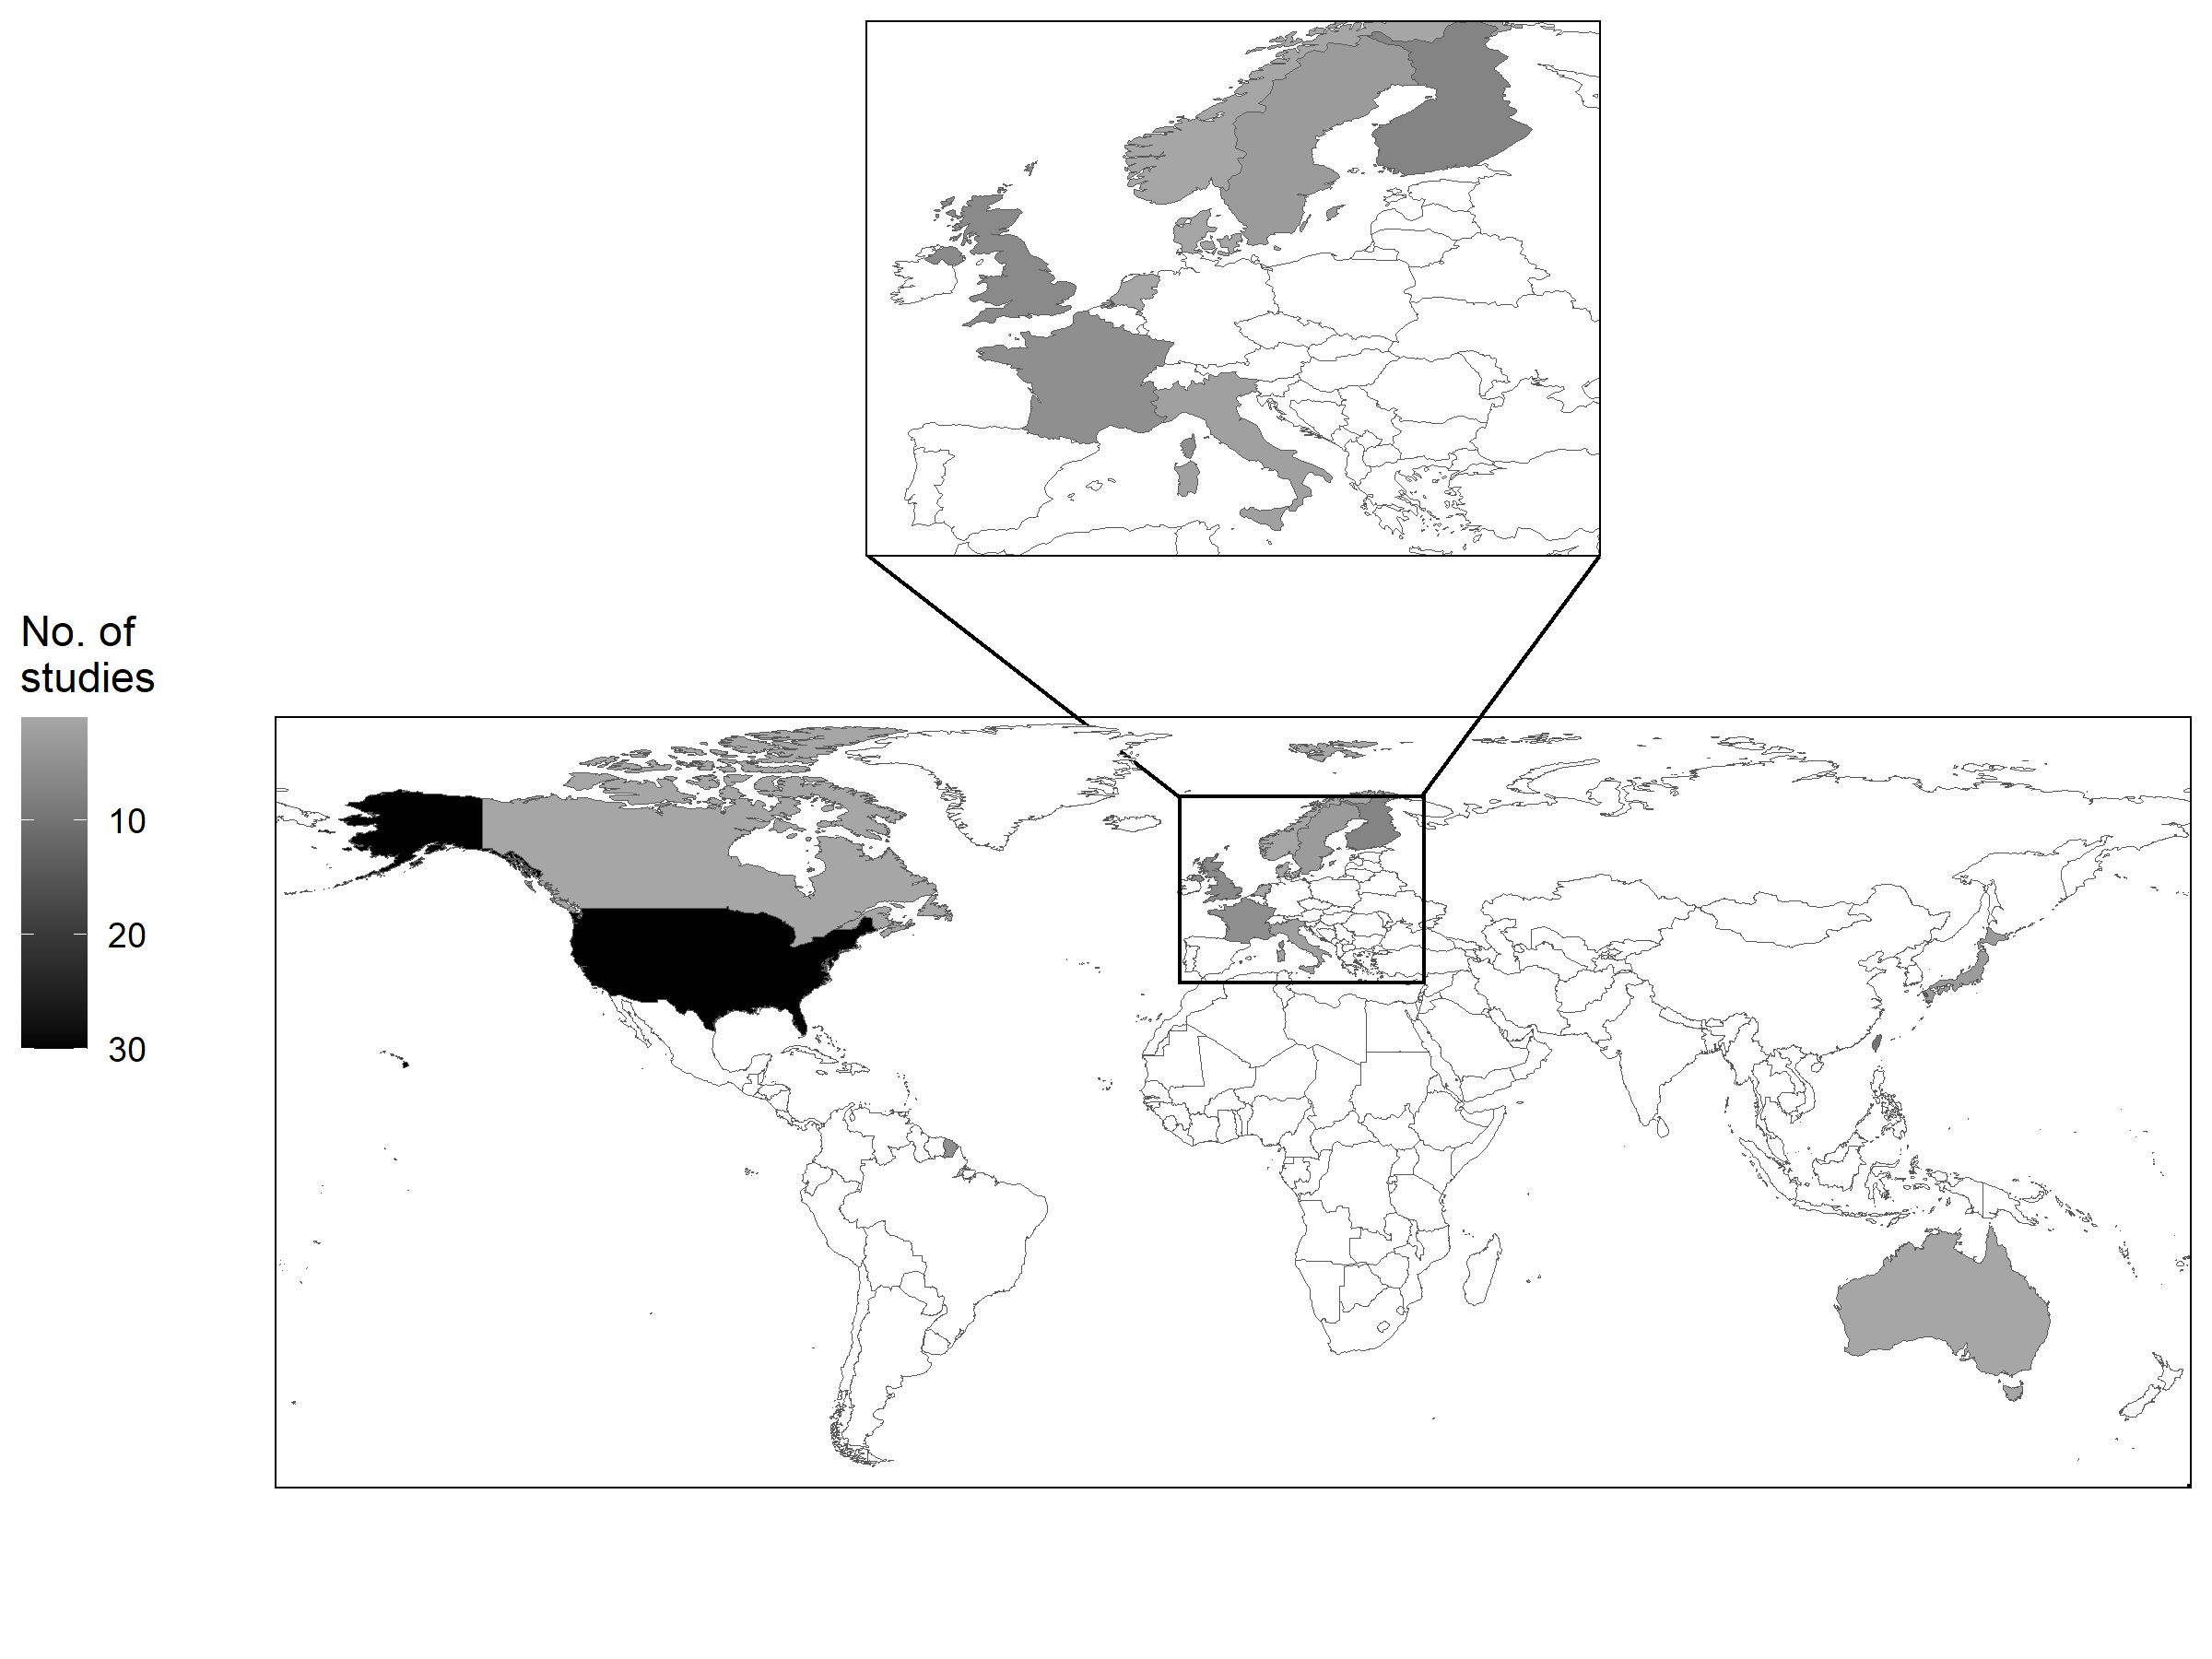
\includegraphics[width=1\linewidth]{figures/sys-rev/cohortLocations} \caption[Geographical distribution of study cohorts]{Geographical distribution of study cohorts}\label{fig:cohortLocations}
\end{figure}

~

Finally, there were several eligible studies reported as conference abstracts that did not present numerical results. These reports were included in the analysis to enable assessment of risk of bias due to missing evidence (see Section \ref{methods-rob-me}).

~

\hypertarget{risk-of-bias-res}{%
\subsection{Risk of bias}\label{risk-of-bias-res}}

As discussed above, the risk-of-bias assessments are presented alongside their corresponding numerical result. A more detailed discussion of the sources and directions of bias is presented in Chapter \ref{tri-heading}, and so this section presents a brief summary of the biases observed in each study design.

For the two randomised controlled trials, both were judged to be at low risk of bias. In contrast, many of the non-randomised studies of statin use were at serious risk of bias due poor controlling for confounding, immortal time bias, and missing outcome data (as noted above, a judgement of low risk of bias for a non-randomised study is rare). Similarly, non-randomised studies of exposures suffered from incomplete adjustment for potentially important confounders, and concerns over the selection of the reported result from among several analyses (e.g.~examination of lipids as a binary or continuous variable). Finally, bias was introduced into Mendelian randomisation studies via the potential for hoziontal pleiotropy and population stratification.\textsuperscript{\protect\hyperlink{ref-davies2018}{69}}

Following best practice, any result judged to be at critical risk of bias should be excluded from any quantitative analyses. Four observational studies were excluded on this basis, predominantly due to a lack of adjustment for any potentially important confounders (i.e.~the study reported unadjusted estimates).\textsuperscript{\protect\hyperlink{ref-mainous2005}{57},\protect\hyperlink{ref-kuo2015}{228},\protect\hyperlink{ref-notkola1998}{232}}

~

\hypertarget{sys-rev-res-Dementia}{%
\subsection{All-cause dementia}\label{sys-rev-res-Dementia}}

\hypertarget{statins}{%
\subsubsection{Statins}\label{statins}}

The two randomised controlled trials provided weak evidence (OR: 1.07, 95\%CI: 0.70-1.66) of an effect on statin use on all-cause dementia risk (Figure \ref{fig:rctStatinDementiaFig}).





\begin{figure}[H]
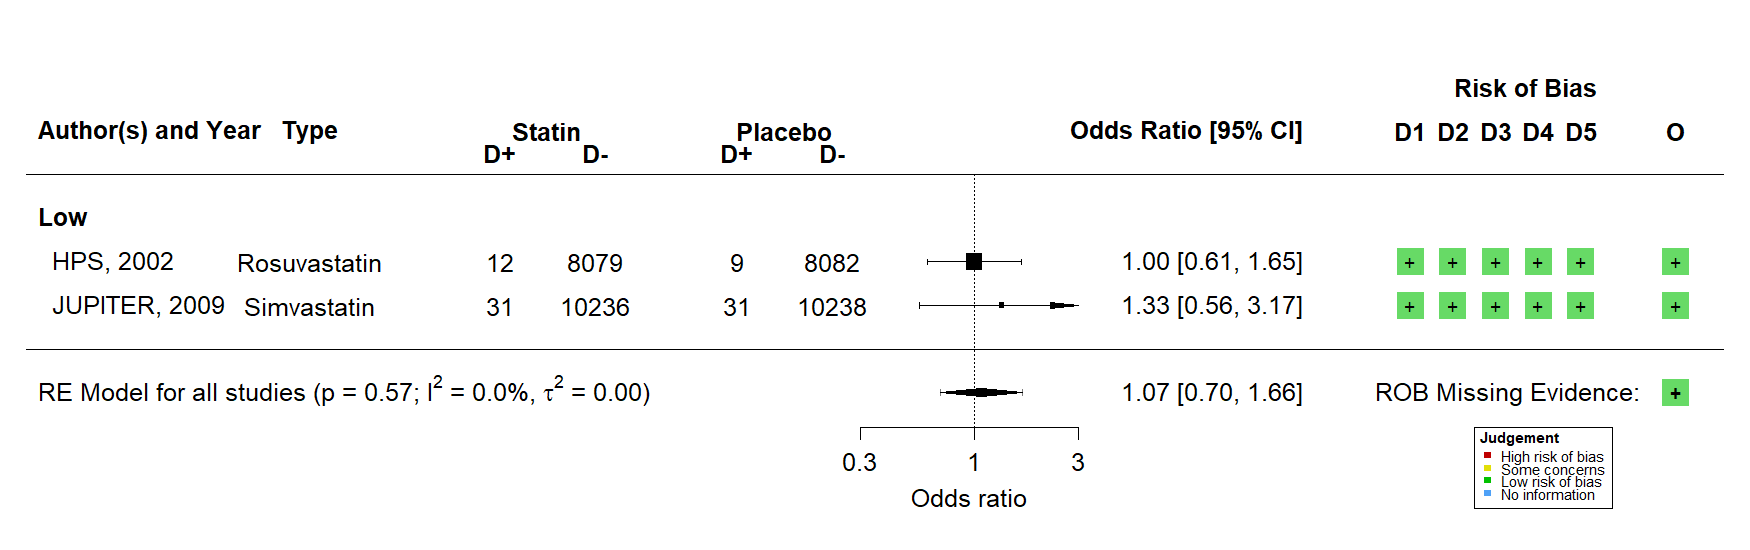
\includegraphics[width=1\linewidth]{figures/sys-rev/fp_rct_statins_Dementia} \caption[Random-effects meta-analysis of statins on all-cause dementia]{Random-effects meta-analysis of randomised controlled trials examining statin statins on all-cause dementia}\label{fig:rctStatinDementiaFig}
\end{figure}

~

In contrast, a meta-analysis of 15 prospective observational studies provided some evidence of a protective effect of statins use on all-cause dementia risk (HR: 0.77, 95\%CI: 0.69-0.87, Figure \ref{fig:obsStatinDementiaFig}).





\begin{figure}[H]
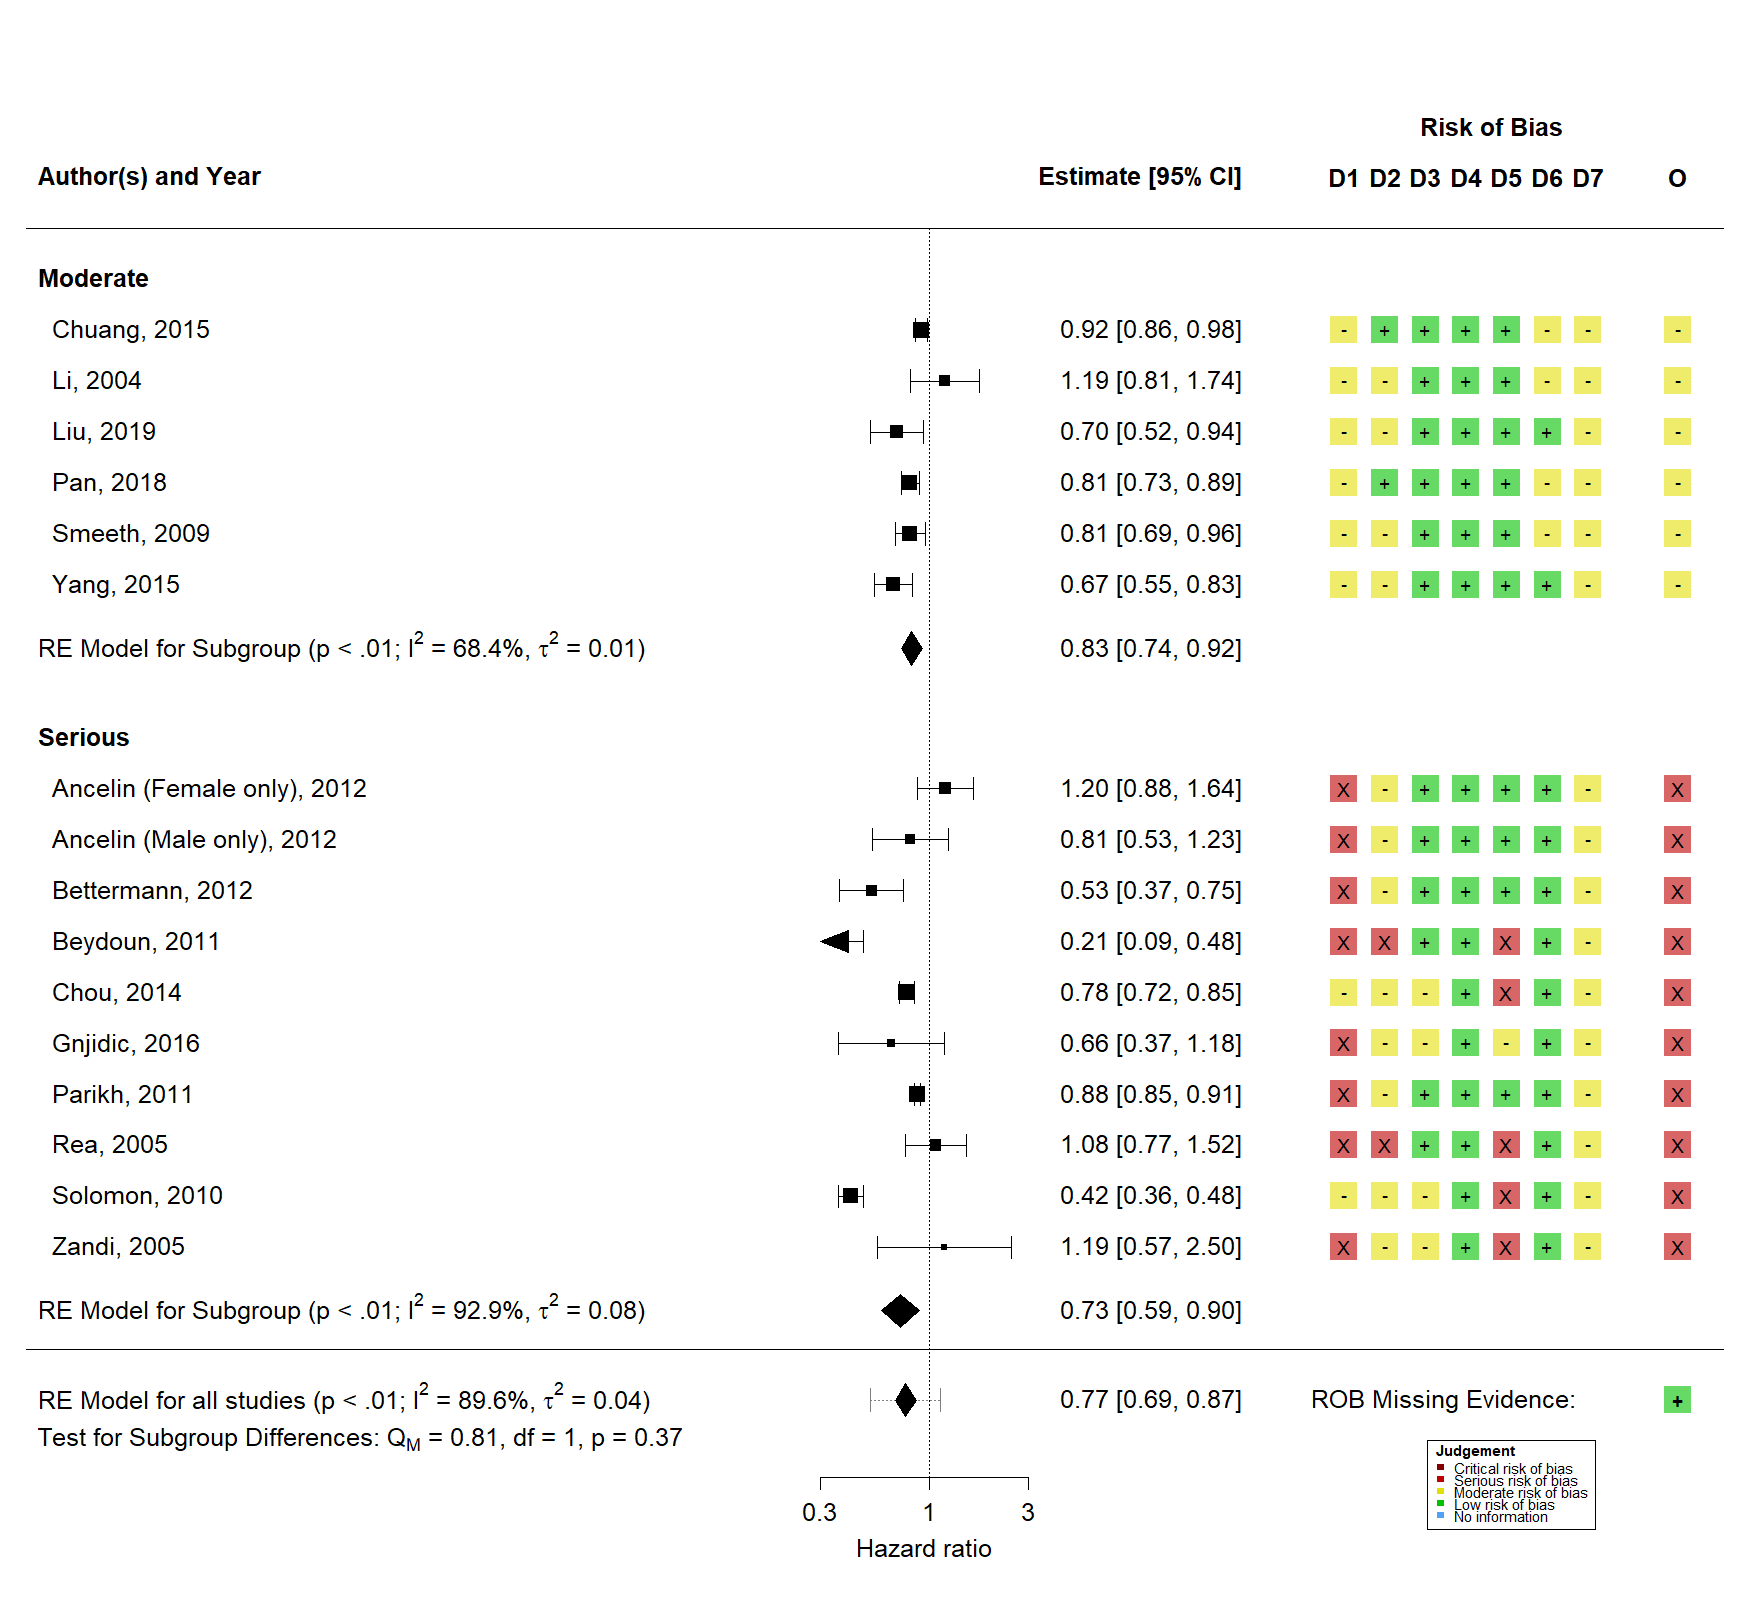
\includegraphics[width=1\linewidth]{figures/sys-rev/fp_obs_Statin-Ever_Dementia} \caption[Random-effects meta-analysis of statins on all-cause dementia]{Random-effects meta-analysis of non-randomised studies examining the effect of statin use on all-cause dementia}\label{fig:obsStatinDementiaFig}
\end{figure}

Finally, a single Mendelian randomisation analysis was identified examining the effect of lowered LDL-c levels on the risk of all-cause dementia via genetic inhibition of the 3-hydroxy-3-methylglutaryl-coenzyme A reductase (HMGCR), emulating statin treatment (see Section \ref{intro-statins} for more details of the statin mechanism of action). This analysis provided weak evidence for an effect (RR: 0.90, 95\%CI: 0.29-2.81).

~

\hypertarget{fibrates}{%
\subsubsection{Fibrates}\label{fibrates}}

Two studies examined the effect of fibrate use on all-cause dementia and found weak evidence for an effect (HR: 0.89, 95\%CI: 0.75-1.07, Figure \ref{fig:obsFibrateDementiaFig}).





\begin{figure}[H]
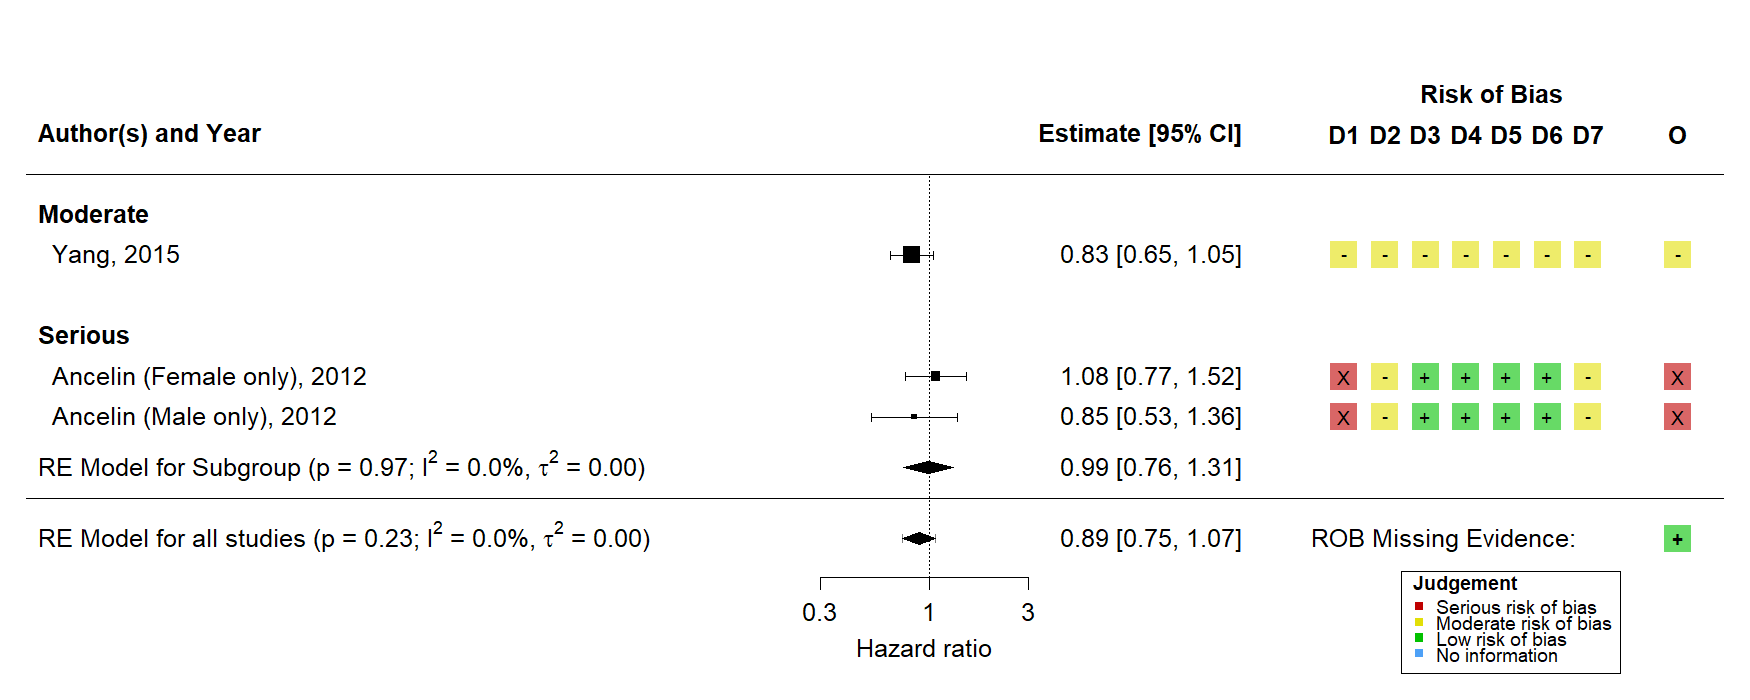
\includegraphics[width=1\linewidth]{figures/sys-rev/fp_obs_Fibrate_Dementia} \caption[Random-effects meta-analysis of statins on all-cause dementia]{Random-effects meta-analysis of non-randomised studies examining the effect of fibrate use on all-cause dementia}\label{fig:obsFibrateDementiaFig}
\end{figure}

\hypertarget{lipids}{%
\subsubsection{Lipids}\label{lipids}}

Across all outcomes, lipid levels were categorised in a number of ways. The most common categorisation was hypercholesterolemia at baseline, defined most frequently as a total cholesterol measurement of greater than 6.5 mmol/L.

Eleven studies reported on the association of hypercholesterolemia with all-cause dementia and provided weak evidence for an effect (HR: 1.11, 95\%CI: 0.98-1.25, Figure \ref{fig:obsHyperDementia}).





\begin{figure}[H]
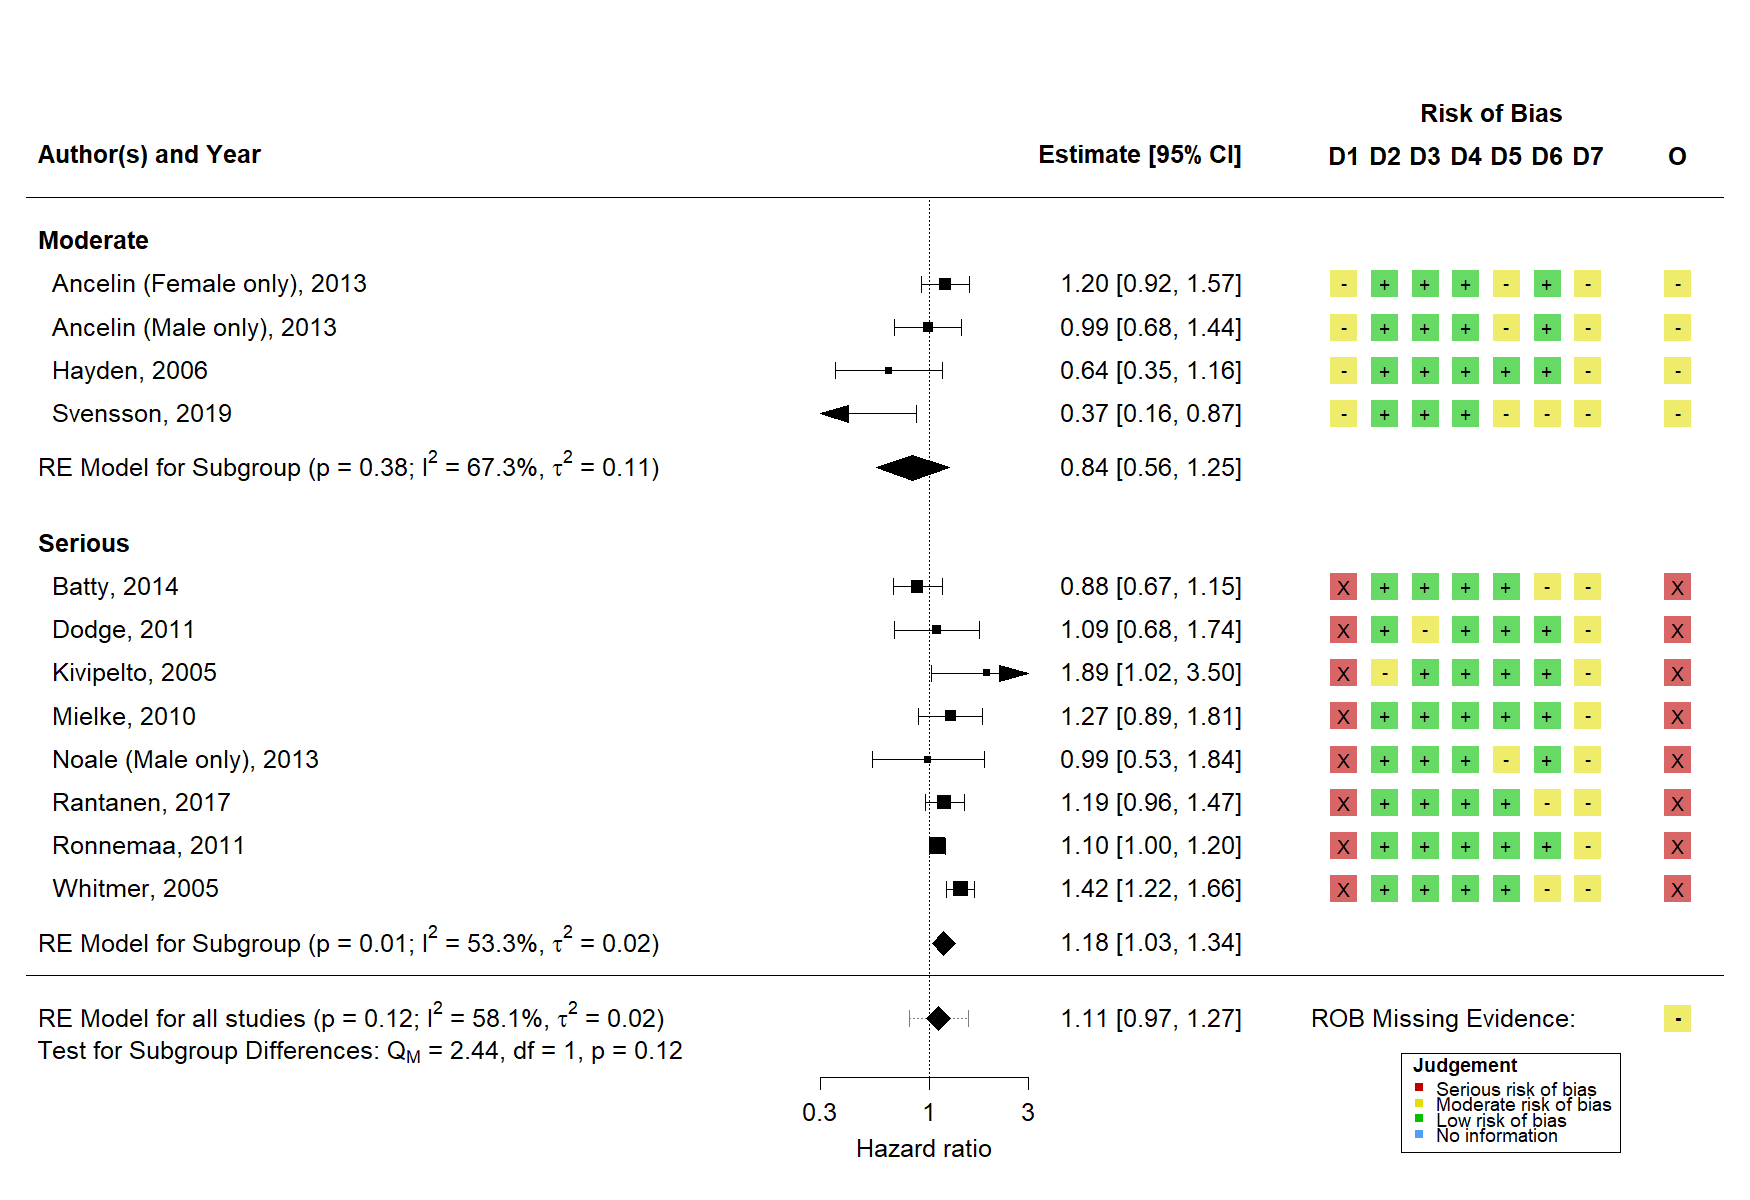
\includegraphics[width=1\linewidth]{figures/sys-rev/fp_obs_hyperchol_Dementia} \caption[Meta-analysis of hypercholesterolemia on all-cause dementia]{Random-effects meta-analysis of non-randomised studies examining the effect of hypercholesterolemia on all-cause dementia}\label{fig:obsHyperDementia}
\end{figure}

Several studies analysed individual lipid fractions by estimating the risk of dementia per 1 standard deviation increase in that fraction (Figure \ref{fig:lipidFractionsDementia}). Weak evidence for an effect on all-cause dementia was found for total cholesterol (N = 5; HR: 0.97, 95\%CI: 0.88-1.07), LDL-c (N = 2; HR: 0.97, 95\%CI: 0.86-1.08), HDL-c (N = 4; HR: 1.05, 95\%CI: 0.96-1.14) and triglycerides (N = 3; HR: 0.90, 95\%CI: 0.74-1.09).





\begin{figure}[H]
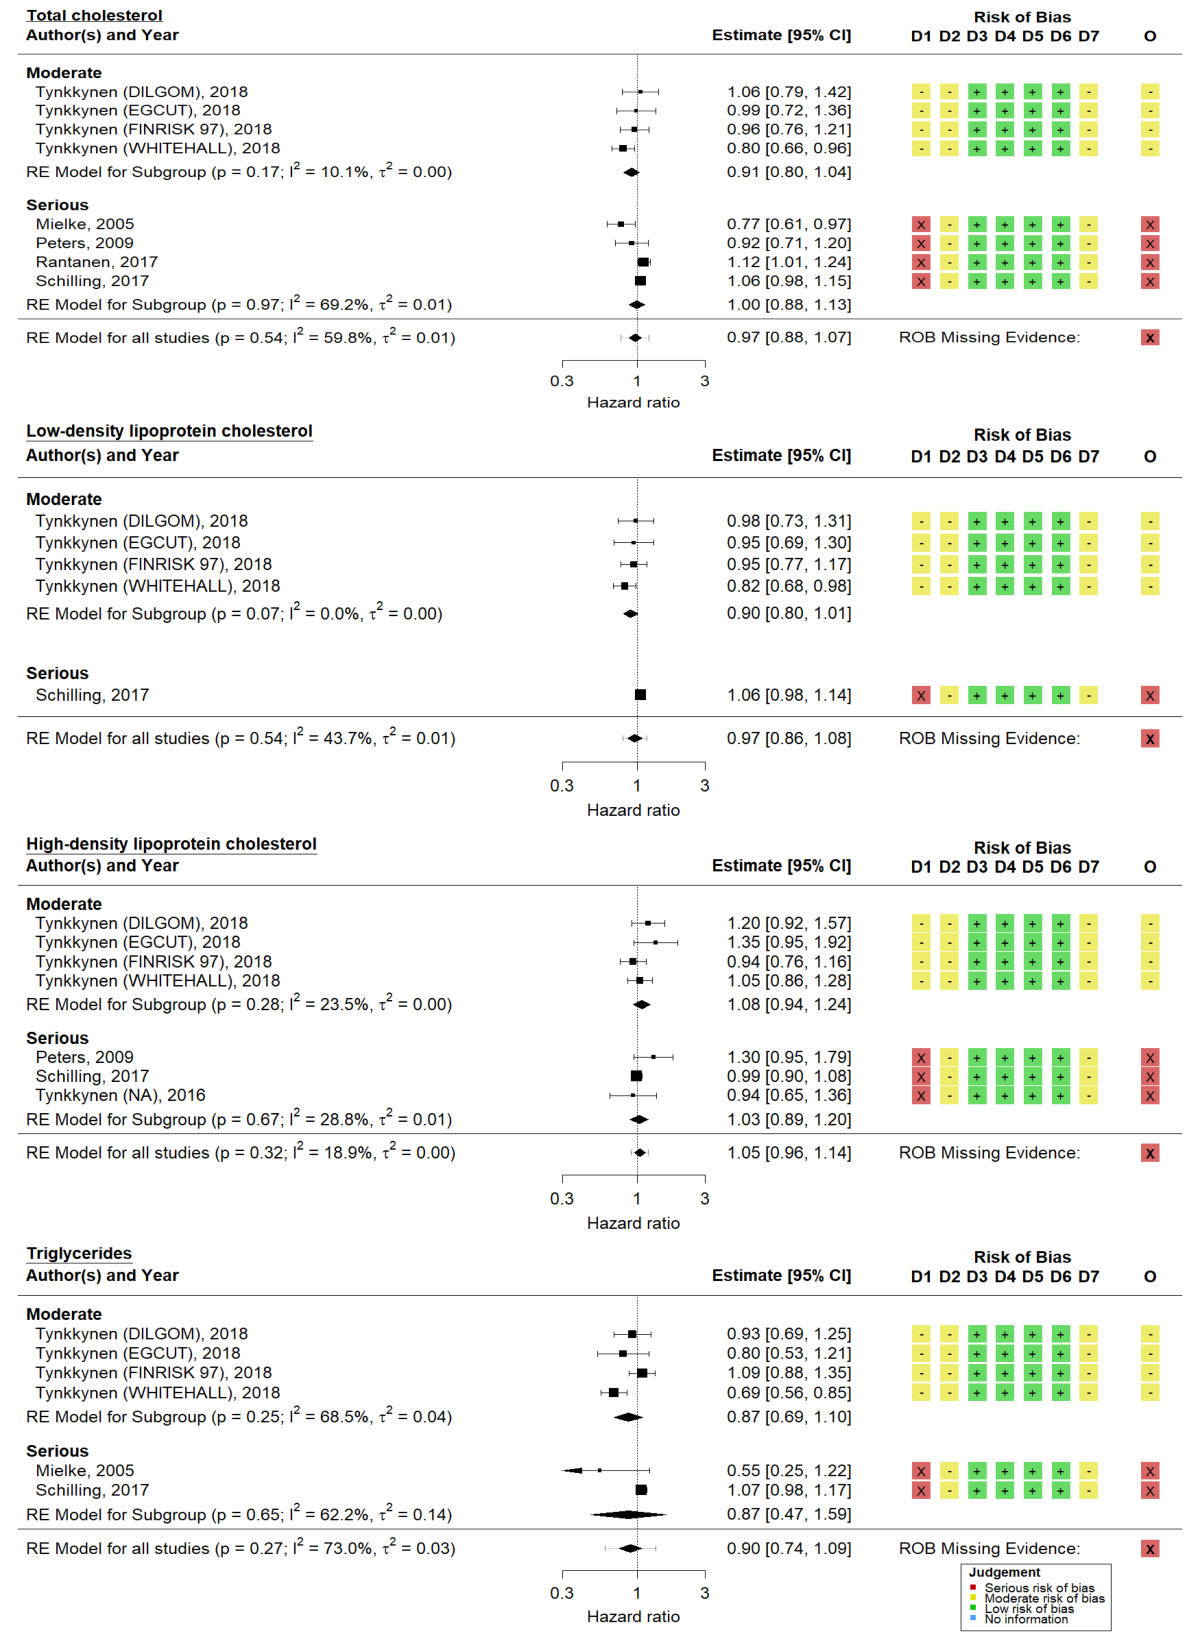
\includegraphics[width=1\linewidth]{figures/sys-rev/fp_lipids_composite_Dementia} \caption[Random-effects meta-analysis of four lipid fractions on all-cause dementia]{Random-effects meta-analysis of four lipid fractions (total cholesteol, HDL, LDL, and triglycerides) on all-cause dementia risk, standardised per 1-SD increase in the lipid fraction.}\label{fig:lipidFractionsDementia}
\end{figure}

Finally, there were no identified Mendelian randomisation analysis examining the effect of lower lipid levels, as determined by any genetic instrument, on all-cause dementia risk.

~

\hypertarget{sys-rev-res-AD}{%
\subsection{Alzheimer's disease}\label{sys-rev-res-AD}}

\hypertarget{statins-1}{%
\subsubsection{Statins}\label{statins-1}}

There were no randomised trials of the use of statins or any other lipid regulating agents on Alzheimer's disease, though several observational studies reported on this outcome and provided evidence for a protective effect (N = 11; HR: 0.83, 95\%CI: 0.69-0.99; Figure \ref{fig:obsStatinADFig}).





\begin{figure}[H]
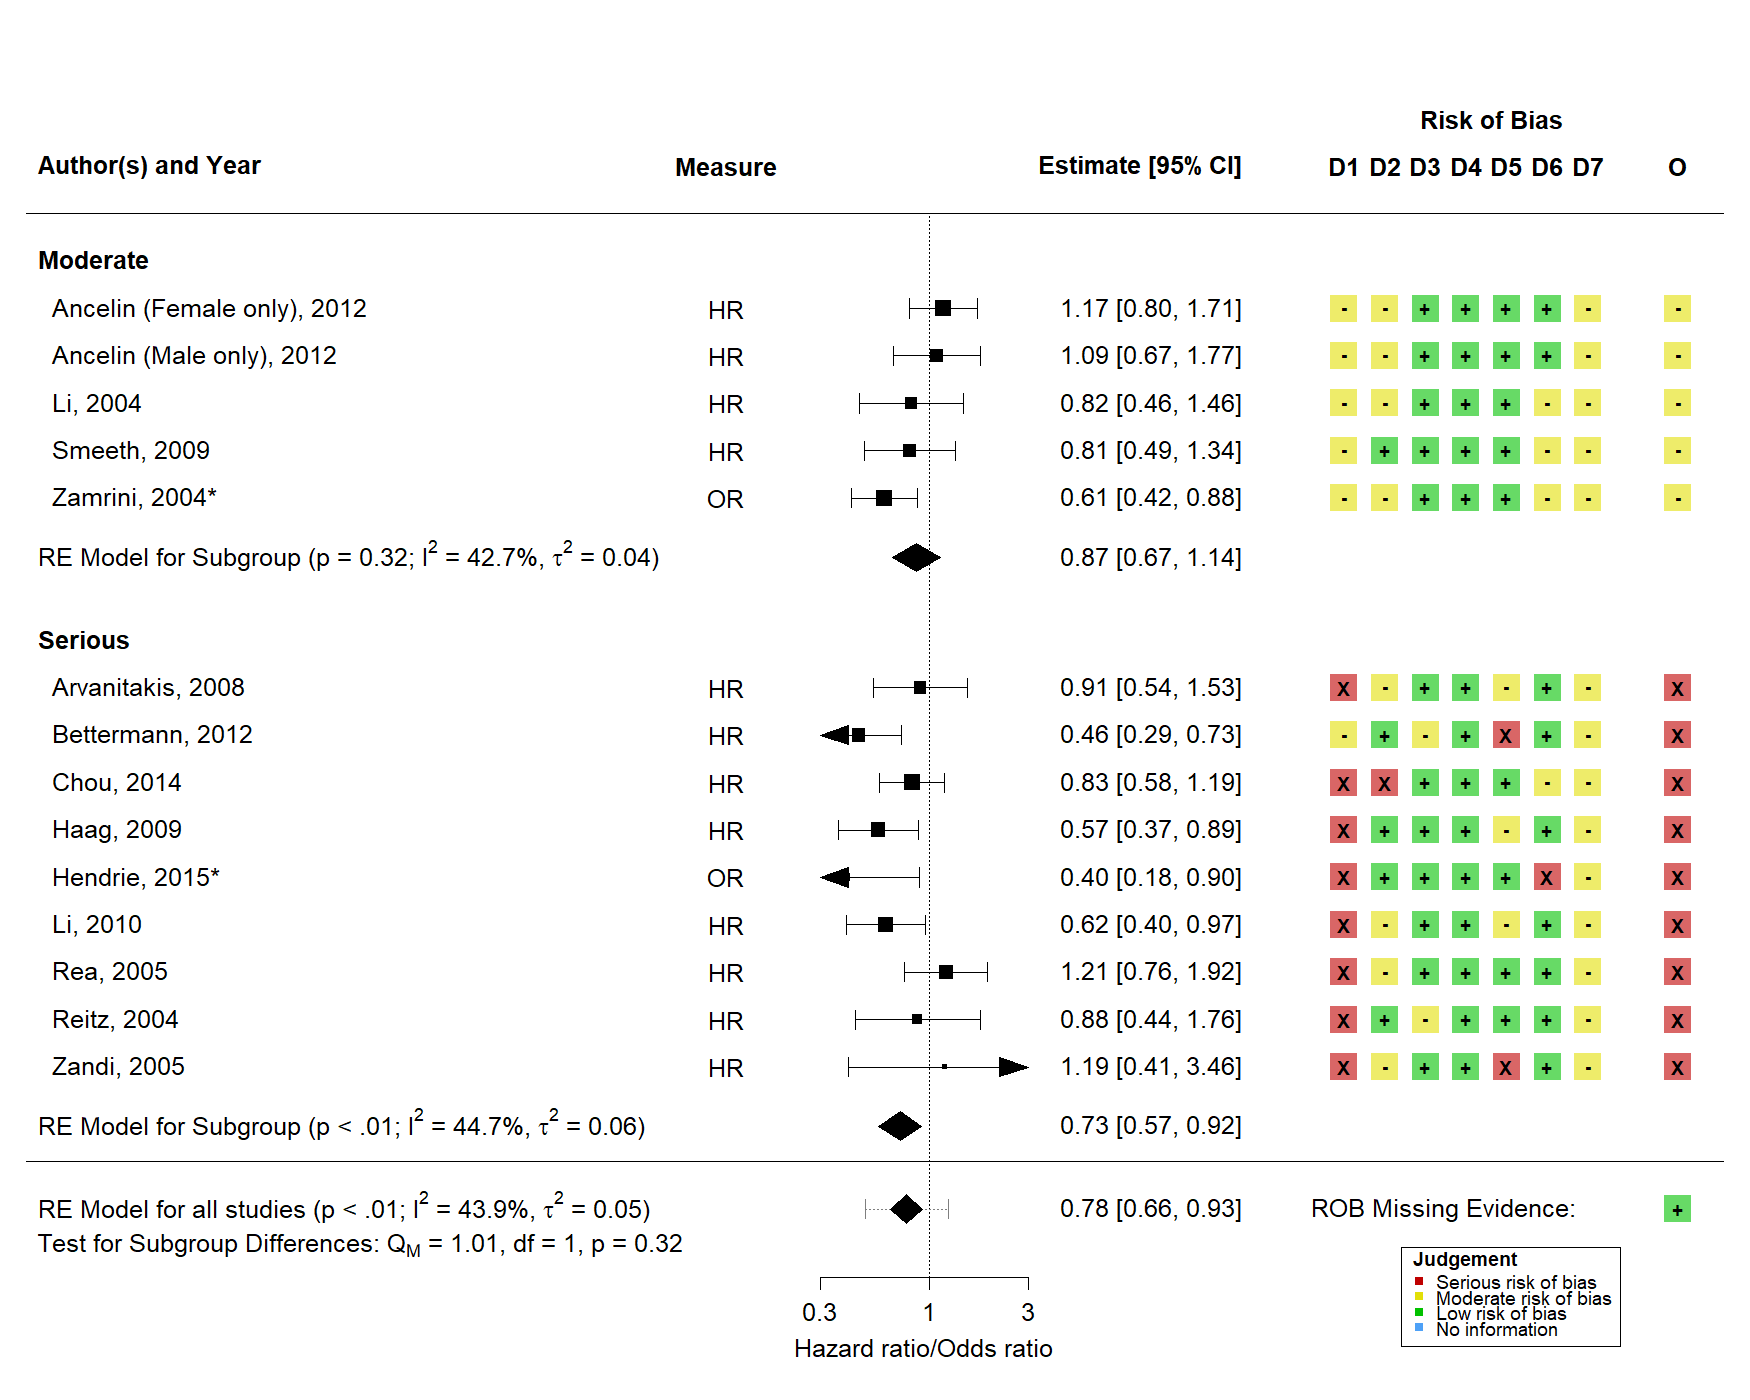
\includegraphics[width=1\linewidth]{figures/sys-rev/fp_obs_Statin-Ever_AD} \caption[Random-effects meta-analysis of statins on Alzheimer's disease]{Random-effects meta-analysis of non-randomised studies examining the effect of statin use on Alzheimer's disease}\label{fig:obsStatinADFig}
\end{figure}

Two Mendelian randomisation studies looked at lipid-lowering specifically as a result of HMGCR inhibition, mediated by SNPs in the gene (rs172338484 and rs12916).\textsuperscript{\protect\hyperlink{ref-benn2017}{73},\protect\hyperlink{ref-so2017}{250}} The first used a one sample approach (SNP-exposure and SNP-outcome associations are estimated using the same dataset) in a large Copenhagen-based cohort, while the second made use of summary level data obtained from the Global Lipids Genetic Consortium (SNP-exposure) and the International Genomics of Alzheimer's Project (SNP-outcome). Meta-analysis of these estimates provided weak evidence of an effect (RR: 0.76, 95\%CI: 0.51-1.14, Figure \ref{fig:mrStatinADFig}).





\begin{figure}[H]
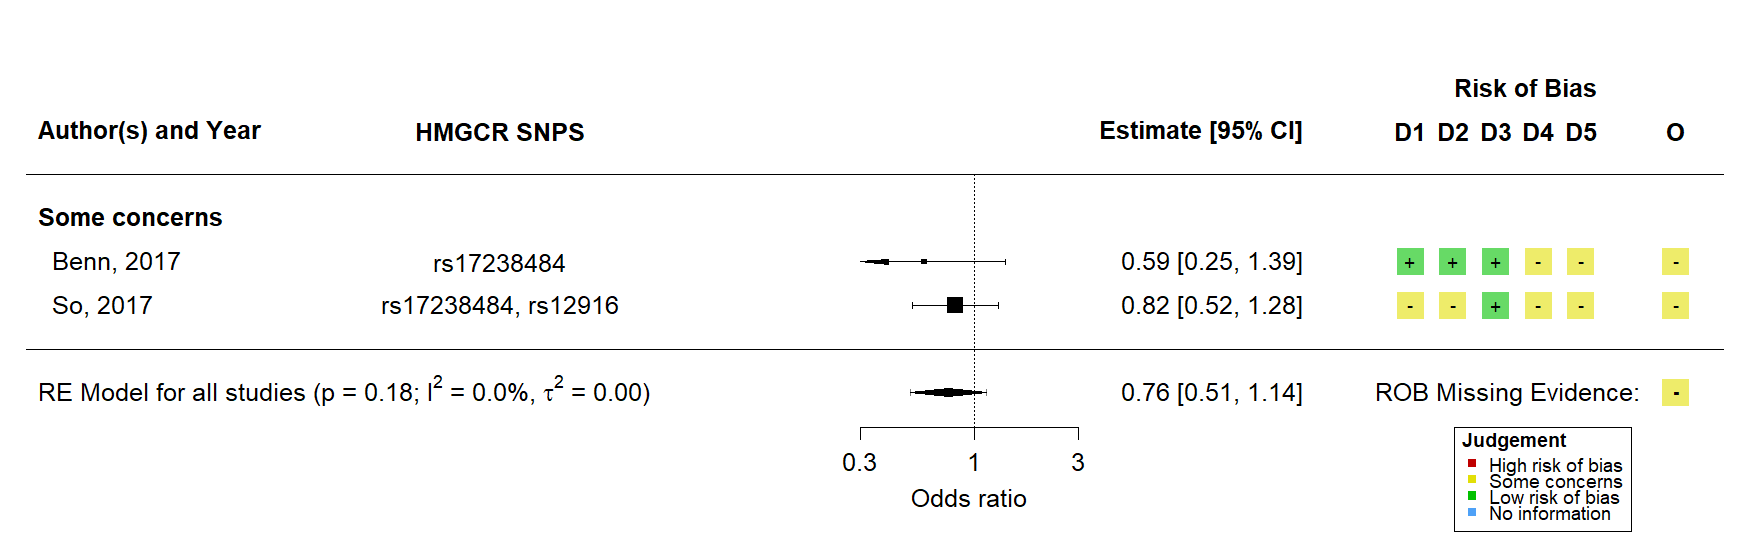
\includegraphics[width=1\linewidth]{figures/sys-rev/fp_MR_HMGCR_AD} \caption[Random-effects meta-analysis of genetically lowered LDL-c via HMGCR inhibition on Alzheimer's disease]{Random-effects meta-analysis of genetically lowered LDL-c via HMGCR inhibition on Alzheimer's disease}\label{fig:mrStatinADFig}
\end{figure}

~

\hypertarget{lipids-1}{%
\subsubsection{Lipids}\label{lipids-1}}

9 studies reported on the association of hypercholesterolemia with all-cause dementia and provided weak evidence for an effect (HR: 0.99, 95\%CI: 0.78-1.25, Figure \ref{fig:obsHyperAD})





\begin{figure}[H]
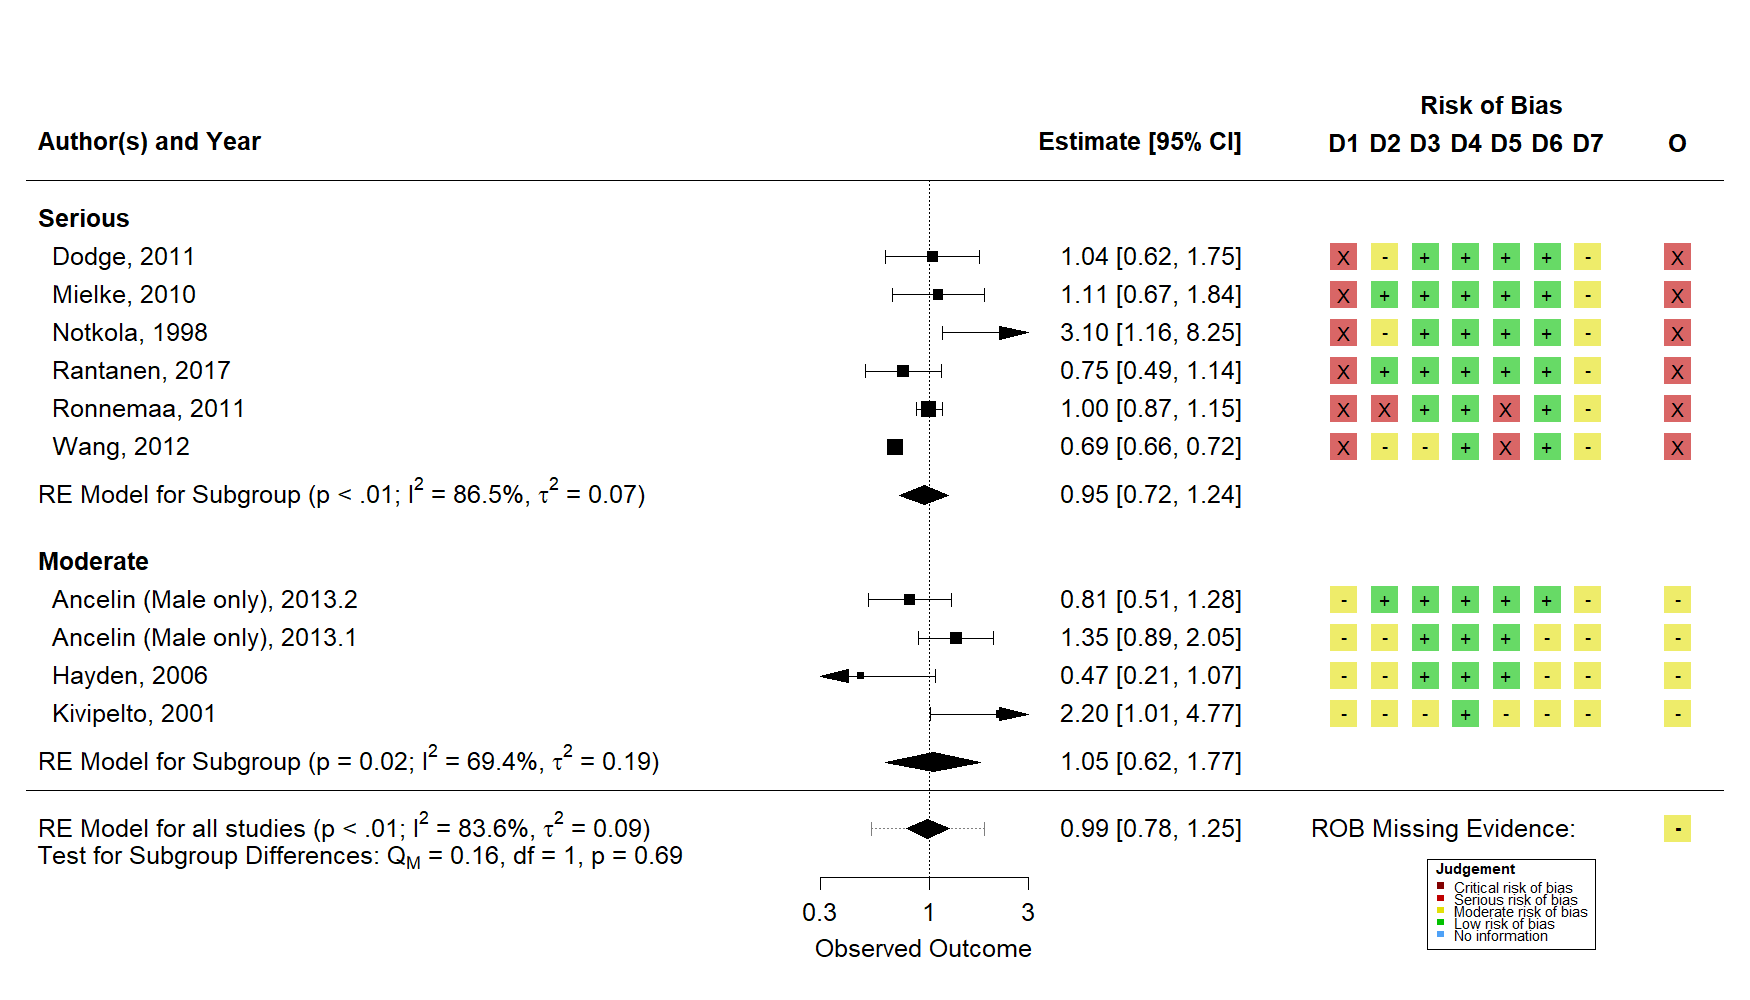
\includegraphics[width=1\linewidth]{figures/sys-rev/fp_obs_hyperchol_AD} \caption[Meta-analysis of hypercholesterolemia on Alzheimer's disease]{Random-effects meta-analysis of non-randomised studies examining the effect of hypercholesterolemia on Alzheimer's disease}\label{fig:obsHyperAD}
\end{figure}

Similarly to all-cause dementia, several studies analysed individual lipid fractions by estimating the risk of dementia per 1 standard deviation increase in that fraction (Figure \ref{fig:lipidFractionsAD}). Weak evidence for an effect on all-cause dementia was found for total cholesterol (N = 5; HR: 1.00, 95\%CI: 0.94-1.06), LDL-c (N = 3; HR: 1.06, 95\%CI: 0.98-1.16), HDL-c (N = 4; HR: 0.99, 95\%CI: 0.91-1.07) or triglycerides (N = 3; HR: 1.00, 95\%CI: 0.84-1.18).





\begin{figure}[H]
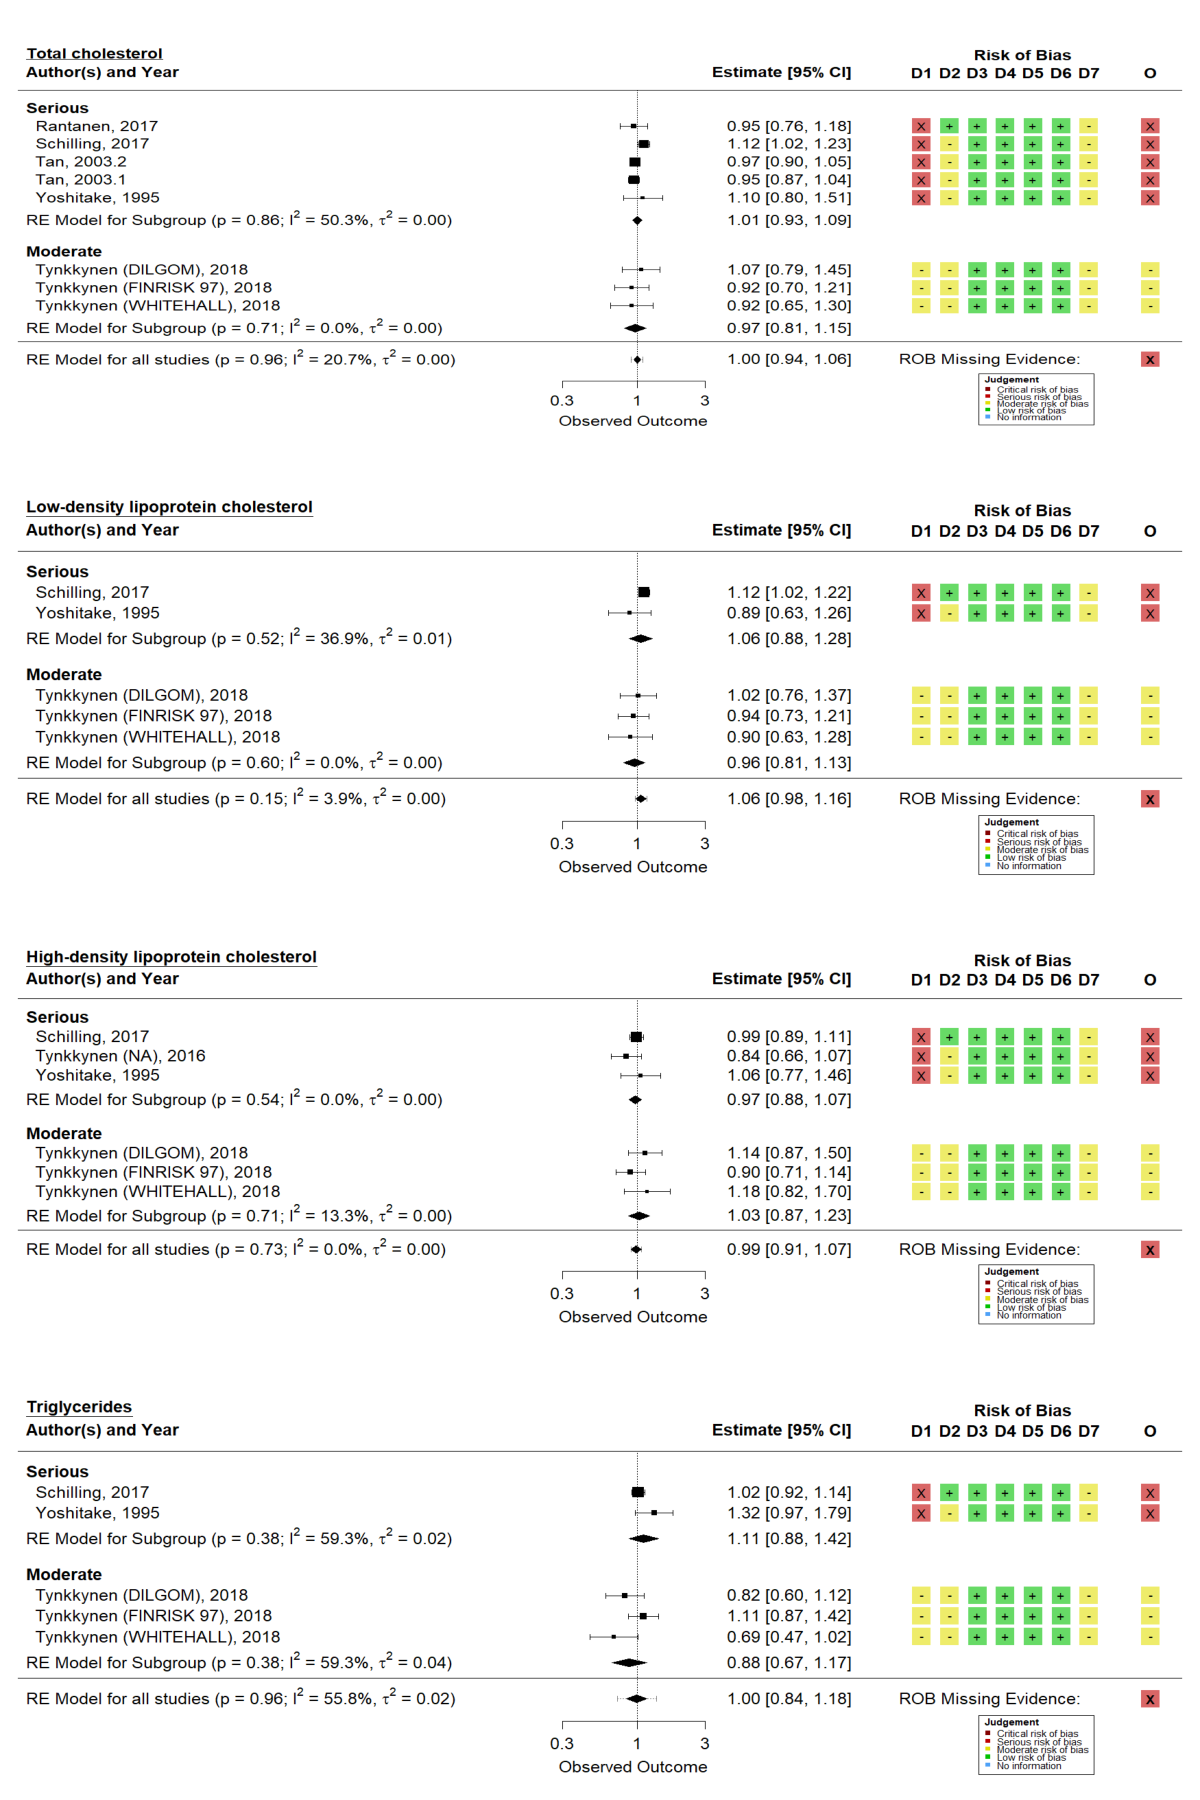
\includegraphics[width=1\linewidth]{figures/sys-rev/fp_lipids_composite_AD} \caption[Random-effects meta-analysis of four lipid fractions on Alzheimer's disease]{Random-effects meta-analysis of LDL on vascular dementia risk, standardised per 1-SD increase in the lipid fraction.}\label{fig:lipidFractionsAD}
\end{figure}

Finally, there were several identified Mendelian randomisation studies examining the effect of genetically lowered LDL-c on Alzheimer's disease risk (Figure \ref{fig:mrDuplication}). However, all of these studies used a two-sample approach, making use of summary statistics from the GLGC and IGAP consortia. Due to this overlap, which would result in a falsely precise estimate caused by multiple counting of the same participants, no meta-analysis of these studies was performed. However, across all analysis, using varying number of SNPS, no evidence for an effect was observed (Figure \ref{fig:mrDuplication}).





\begin{figure}[H]

{\centering 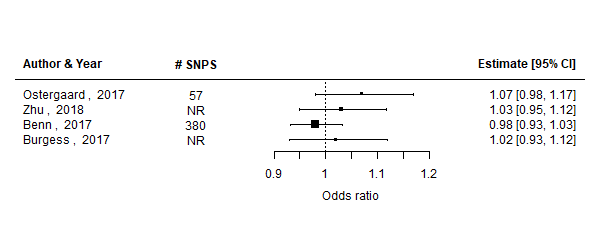
\includegraphics[width=0.8\linewidth]{figures/sys-rev/mrDuplication} 

}

\caption[Summary of duplication across two sample Mendelian randomisation studies]{Summary of duplication across Mendelian randomisation studies which used summary statistics from the Global Lipid Genetics Consortium (GLGC) and the International Genomics of Alzheimer's Project (IGAP). Note that the Alzheimer's Disease Genetics Consortium (ADGC) is a sub-cohort within IGAP.}\label{fig:mrDuplication}
\end{figure}

~

\hypertarget{sys-rev-res-VaD}{%
\subsection{Vascular dementia}\label{sys-rev-res-VaD}}

\hypertarget{statins-2}{%
\subsubsection{Statins}\label{statins-2}}

As noted in Section \ref{sys-rev-characteristics} above, there was substantially less literature available on the association of my risk factors of interest and vascular dementia. There were no available randomised trials for this outcome. Three prospective cohort studies examined statin use and vascular dementia, though meta-analysis of these studies provided weak evidence for an effect (N = 3; HR: 0.99, 95\%CI: 0.79-1.25; Figure \ref{fig:obsStatinVaDFig}).





\begin{figure}[H]
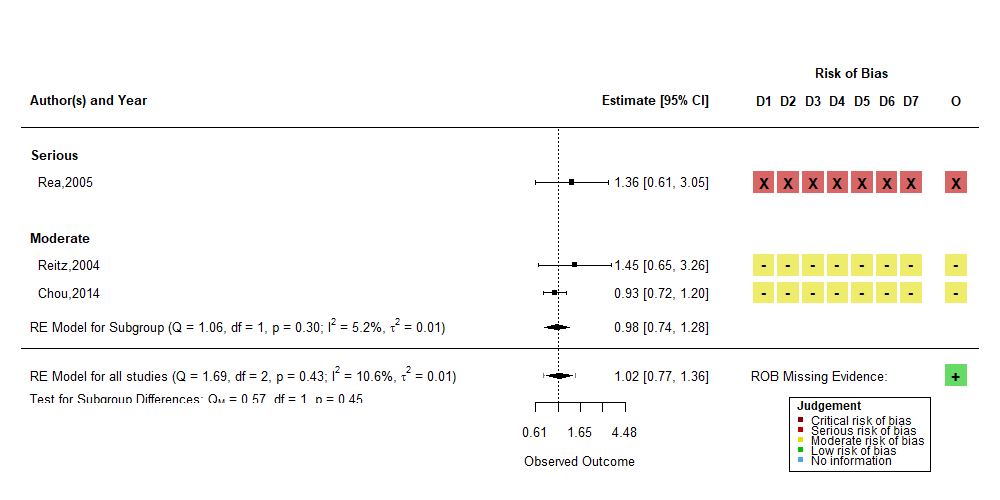
\includegraphics[width=1\linewidth]{figures/sys-rev/fp_obs_Statin-Ever_VaD} \caption[(ref:obsStatinDVaD-scap)]{Random-effects meta-analysis of non-randomised studies examining effect of statin use on vascular dementia}\label{fig:obsStatinVaDFig}
\end{figure}

A single Mendelian randomisation analysis was identified that examining the effect of genetically lowered LDL-c levels via HMGCR inhibition on the risk of vascular dementia, which provided weak evidence for an effect (RR: 0.44, 95\%CI: 0.21-0.91).

~

\hypertarget{lipids-2}{%
\subsubsection{Lipids}\label{lipids-2}}

Three studies reported on the association of hypercholesterolemia with vascular dementia and provided weak evidence for an effect (HR: 1.20, 95\%CI: 1.00-1.44, Figure \ref{fig:obsHyperVaD})





\begin{figure}[H]
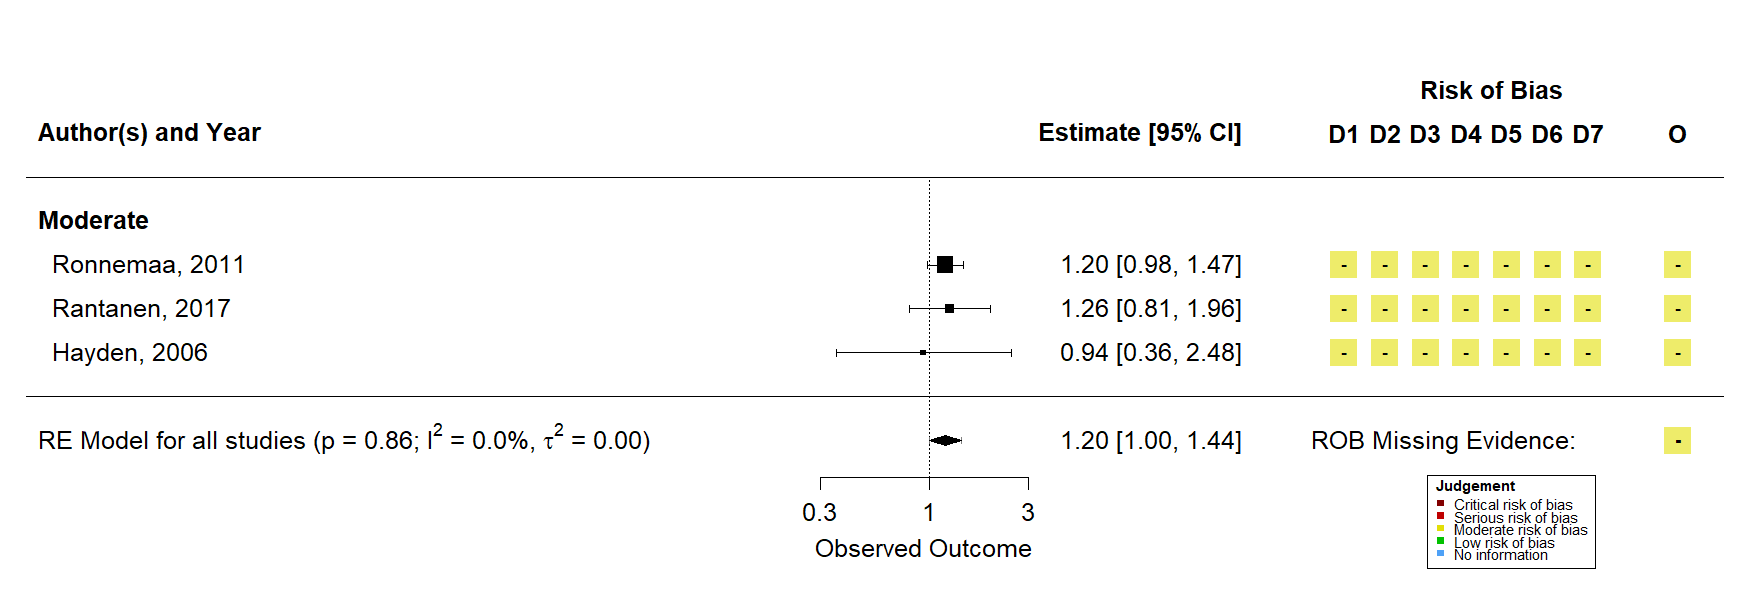
\includegraphics[width=1\linewidth]{figures/sys-rev/fp_obs_hyperchol_VaD} \caption[Meta-analysis of hypercholesterolemia on vascular dementia]{Random-effects meta-analysis of non-randomised studies examining the effect of hypercholesterolemia on vascular dementia}\label{fig:obsHyperVaD}
\end{figure}

Few studies investigated the effect of individual lipid fractions. Only for total cholesterol was there greater than one result reported (Figure \ref{fig:lipidFractionsVaD}), and a meta-analysis of these found weak evidence for an effect (N = 2; HR: 1.05, 95\%CI: 0.79-1.41). A single study provided evidence on the other three fractions,\textsuperscript{\protect\hyperlink{ref-yoshitake1995}{245}} and similar found minimal evidence of an effect LDL-c (N = 1; HR: 1.12, 95\%CI: 0.83-1.51), HDL-c (N = 1; HR: 0.83, 95\%CI: 0.60-1.14) or triglycerides (N = 1; HR: 1.00, 95\%CI: 0.75-1.34).





\begin{figure}[H]
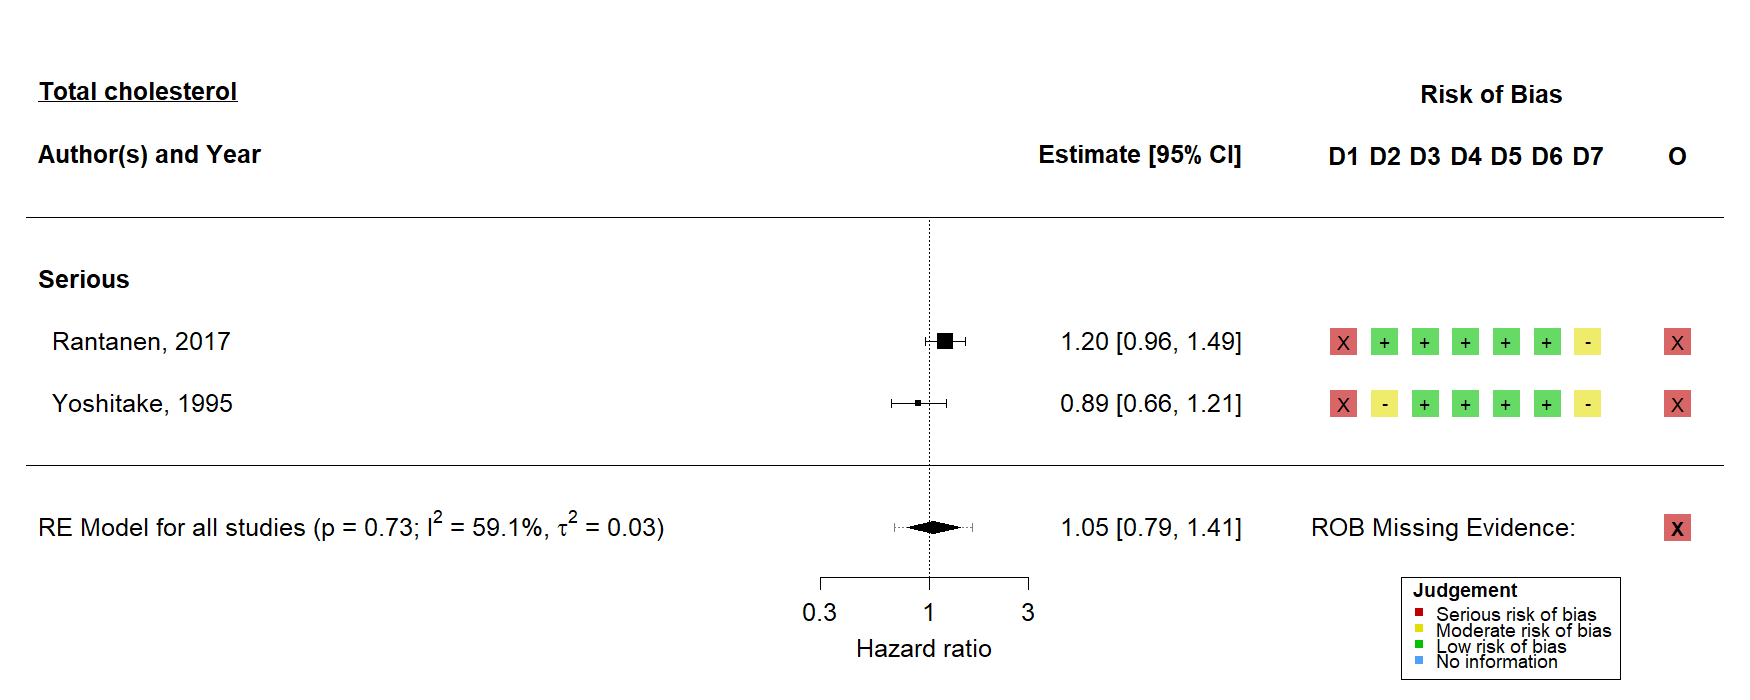
\includegraphics[width=1\linewidth]{figures/sys-rev/fp_obs_VaD_TC_} \caption[Random-effects meta-analysis of four lipid fractions on Alzheimer's disease]{Random-effects meta-analysis of LDL on vascular dementia risk, standardised per 1-SD increase in the lipid fraction.}\label{fig:lipidFractionsVaD}
\end{figure}

Finally, no Mendelian randomisation analyses examining the effect of genetically determined lipid levels on vascular dementia risk were identified.

~

\hypertarget{dose-response-results}{%
\subsection{Dose response meta-analysis of lipid levels}\label{dose-response-results}}

There were 13 studies that were eligible for dose-response meta-analysis as they provide several categories of lipid exposure. However, following data extraction, five were excluded as they did not reported the relevant information needed (most commonly, the cut-off measures for each category).

Across the remaining eight studies, a sufficient number of studies (n \(\geqslant\) 3) were identified only for the total cholesterol-Alzheimer's, LDL-Alzheimer's, and total cholesterol-dementia strata. This analysis provided weak evidence for a non-linear effect of lipid levels on dementia outcomes, and Figure \ref{fig:lipidsDoseResponse} illustrates this for the total cholesterol-Alzheimer's strata. Similar figures for the other analysed lipid-outcome strata are presented in Appendix \ref{hold}.





\begin{figure}[H]

{\centering 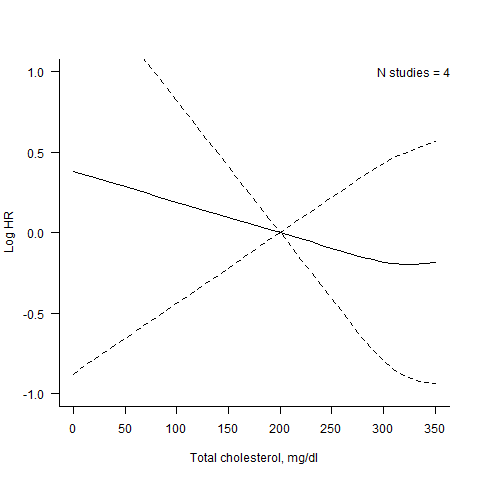
\includegraphics[width=0.7\linewidth]{figures/sys-rev/dr_AD_TC} 

}

\caption[Dose-response meta-analysis of total cholesterol]{Dose-response meta-analysis of total cholesterol on Alzheimer's disease}\label{fig:lipidsDoseResponse}
\end{figure}

~

\hypertarget{additional-analyses-1}{%
\subsection{Additional analyses}\label{additional-analyses-1}}

Investigation of potential sources of heterogeneity was complicated by two factors. In the first instance, few meta-analysis included more than 10 results, the recommended minimum required for meta-regression. Secondly, poor reporting of summary statistics including education level and baseline cognitive ability precluded the use of several results in a meta-regression analysis.

Age and sex were assessed as potential causes of heterogeneity in the meta-analyses of statin use and hypercholesterolemia on all cause dementia and Alzheimer's disease, but I found weak evidence for variation in the observed effect estimates due to these factors.

Similarly, assessment of small-study effects, for which publication bias could be one potential reason, was hindered by the relatively small number of results included in a given meta-analysis. However, all analyses assessed provided weak evidence of small-study effects.

~

~

\hypertarget{missing-evidence}{%
\subsection{Missing evidence}\label{missing-evidence}}

The risk of bias due to missing evidence in each synthesis is shown beside the overall summary diamond in each forest plot presented above. For randomised controlled trials and non-randomised studies of interventions, the risk of bias due to missing evidence was assessed to be minimal. However, there was substantial evidence that results were selectively reported in studies examining the effect of lipid fractions on dementia outcomes (Figures \ref{fig:lipidFractionsDementia}, \ref{fig:lipidFractionsAD} and \ref{fig:lipidFractionsVaD}).

~

\hypertarget{sys-rev-including-preprints-res}{%
\subsection{Added evidential value of including preprints}\label{sys-rev-including-preprints-res}}

As show in Figure \ref{fig:prisma-flow-fig}, the number of hits returned by the preprint searching was not substantial (bioRxiv = 256, medRxiv = 0). From these hits, three preprinted reports of eligible studies were included in the review, of which two described unique studies not captured by the main search.\textsuperscript{\protect\hyperlink{ref-so2017}{250},\protect\hyperlink{ref-andrews2019}{252}}

One preprint (So \emph{et al}\textsuperscript{\protect\hyperlink{ref-so2017}{250}}) provided additional evidential value in a single meta-analysis (5.6\% of all meta-analyses performed in this chapter). This meta-analysis of Mendelian randomisation studies examined the effects of lipid-lowering via HMGCR mutations on incidence of Alzheimer's disease (Figure \ref{fig:mrStatinADFig}. To assess the evidence added to the meta-analysis through inclusion of the preprint, the data were re-analysed using a fixed-effect model. Examination of the weight assigned to each result in the analysis illustrates that a large proportion (78\%) of the weight is given to the preprinted result. However, the inclusion of the preprinted study did not have a substantial impact on the results (RR: 0.76, 95\%CI: 0.51-1.14) versus the single published study (RR: 0.59, 95\%CI: 0.25-1.39).

The other two preprints identified\textsuperscript{\protect\hyperlink{ref-andrews2019}{252},\protect\hyperlink{ref-zhu2017}{253}} reported on the effect of LDL-c on Alzheimer's disease using data from GLCC and IGAP consortia. As illustrated in Figure \ref{fig:mrDuplication}, these consortia were previously analysed in several published reports, and so these preprints did not add to the evidence base.

Investigation of the publication status of the two preprints reporting studies not also identified by the main search after a two-year lag found that one had been subsequently published in late 2019.\textsuperscript{\protect\hyperlink{ref-andrews2021}{247},\protect\hyperlink{ref-andrews2019}{252}} The final preprint has not yet been published.\textsuperscript{\protect\hyperlink{ref-so2017}{250}}

~

\hypertarget{discussion-1}{%
\section{Discussion}\label{discussion-1}}

This review has presented a summary of the available evidence on the association between lipids, and treatments that modify lipids such as statins, and the subsequent risk of dementia. This discussion seeks to summarise the key findings in terms of literature sources and results as reported. A detailed comparison across the evidence sources, exposure measures and sources of bias reported here is presented as part of the triangulation exercise in Chapter \ref{tri-heading}.

~

\hypertarget{summary-of-findings}{%
\subsection{Summary of findings}\label{summary-of-findings}}

There was some indication of a protective effect of statins on all-cause and Alzheimer's disease dementia when looking at solely at observational studies. This finding was not supported by evidence from the two available RCTs, or by studies that emulated statin treatment using a genetic proxy, suggesting that these findings may be a result of heterogeneity in exposure (e.g.~mid-life lipid lowering in non-randomised studies versus life-course lipid exposure in Mendelian randomisation studies and late-life lipid reduction in RCTs) or alternatively due to biases within the non-randomised studies.

Across dementia outcomes, the majority of studies were non-randomised studies of lipids, or treatments that affect lipid levels such as statins. This distribution of evidence between analytical designs is to be expected. Randomised controlled trials of dementia are particularly challenging, as the long follow-up made necessary by the long latent period of the condition, makes trials logistically challenging and financial expensive. Similarly, Mendelian randomisation is a comparatively new study design (as illustrated in Figure \ref{fig:typeByYear}), which appears in the literature in recent years, driven by the availability of summary genome wide association studies (GWAS) that form the basis of the two-sample Mendelian randomisation approach.

~





\begin{figure}[H]
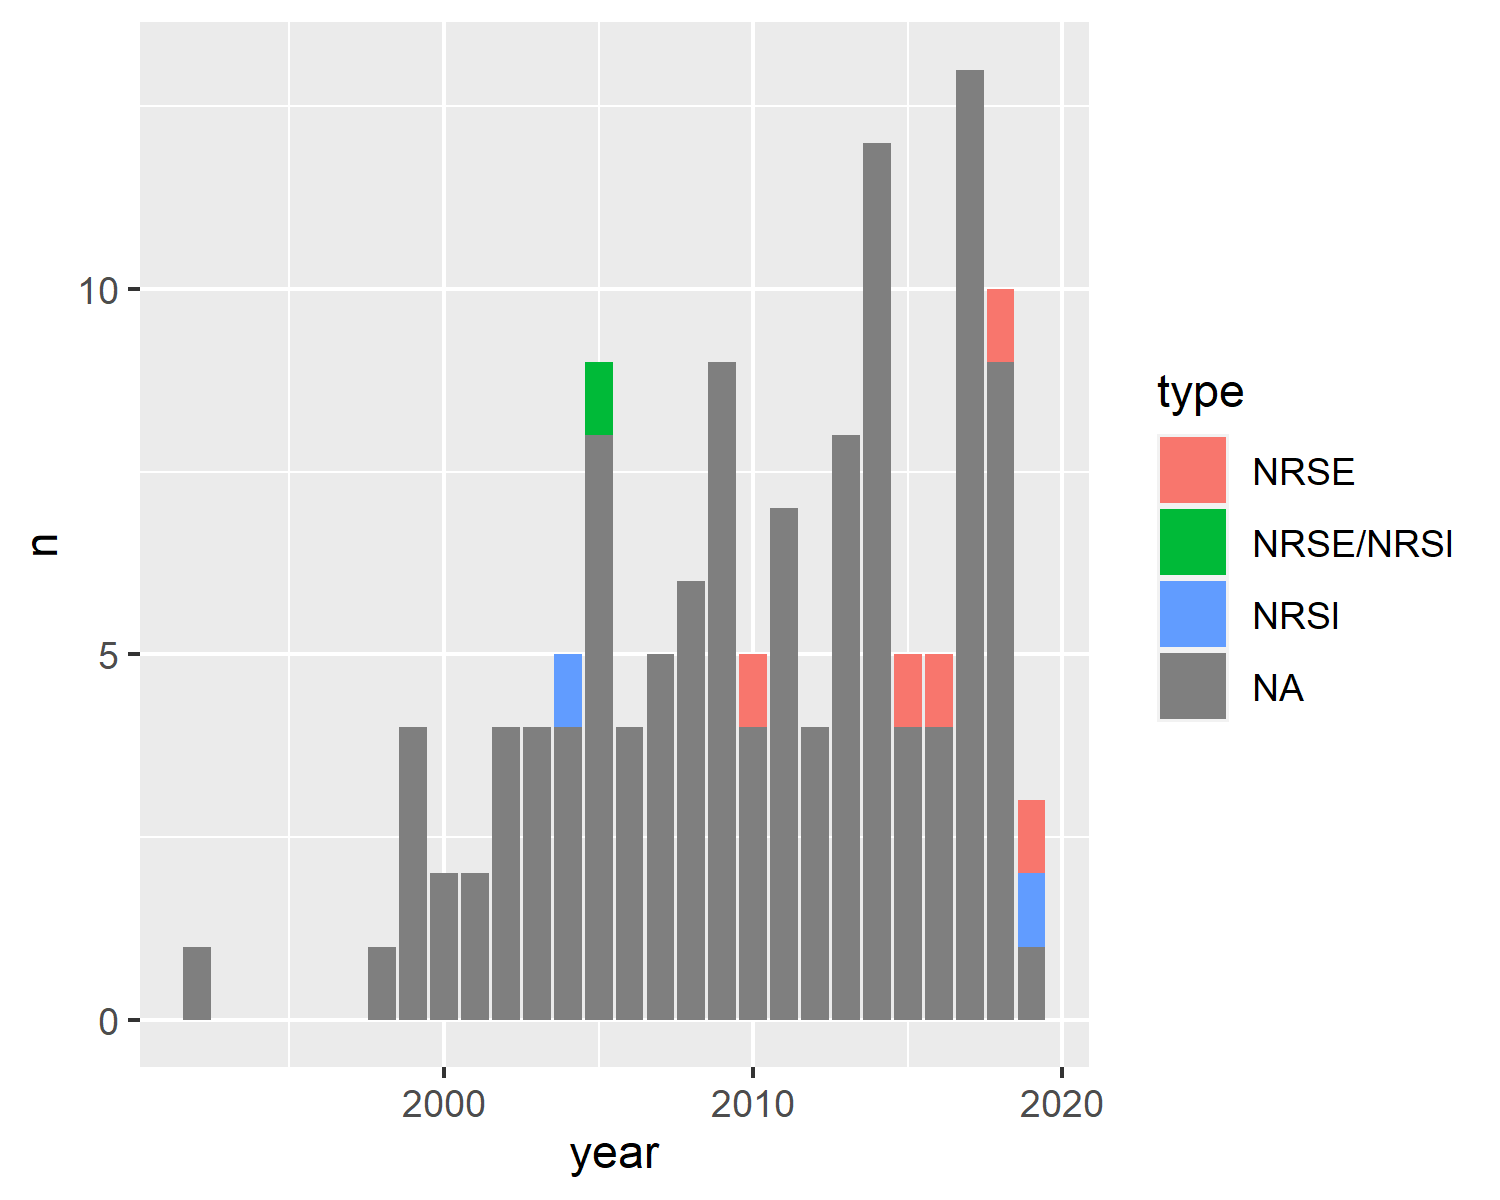
\includegraphics[width=1\linewidth]{figures/sys-rev/type_by_year} \caption[Study designs by year of publication]{Included study designs for any dementia outcome by year of publication}\label{fig:typeByYear}
\end{figure}

~

A common theme was an absence of studies examining vascular dementia as an outcome, most noticeable when comparing the evidence base for statins in dementia/Alzheimer's (Figures \ref{fig:obsStatinDementiaFig} \& \ref{fig:obsStatinADFig}) with that available for vascular dementia (Figure \ref{fig:obsStatinVaDFig}). This is particularly interesting given that lipids and statins are strongly related to the prevention of vascular disease. A potential explanation for this observation may be publication bias or the ``file-drawer effect'',\textsuperscript{\protect\hyperlink{ref-rosenthal1979}{83}} though there was weak evidence of a small-study effects for this outcome (of which publication bias is a potential cause).\textsuperscript{\protect\hyperlink{ref-sterne2011}{178}} Similarly, only one Mendelian randomisation studies examined this outcome, primarily because of the absence (until recently) of vascular dementia GWAS which precludes a two-sample approach.

Of note, this review did not include the commonly cited PROSPER RCT, which examined the effect of pravastatin on CVD risk, reporting on cognitive outcomes as one of several secondary outcomes.\textsuperscript{\protect\hyperlink{ref-shepherd2002}{255}} While widely cited in relation to the effect of statins on dementia risk and included in the Cochrane review of RCTs on this topic,\textsuperscript{\protect\hyperlink{ref-mcguinness2016}{64}} the trial reported solely on the change in a range of cognitive measures (MMSE, Stroop test, Picture-Word Learning test and others) over follow-up. Though a useful indicator of general cognitive decline, it is not equivalent to a dementia diagnosis using recognised criteria as cognitive tests should feed into a broader diagnostic pathway (see Section \ref{diagnostic-criteria}). As such, this trial did not meet the inclusion criteria for this review.

Risk of bias across the individual results was generally quite high. The causes and expected impact of these biases on the results are discussed in more detail in Chapter \ref{tri-heading}. Of particular interest to this chapter, however, was the high risk of bias due to missing evidence observed for observational studies of lipid levels. In many cases, estimates were known to be missing from meta-analyses not at random due to preferential reporting of significant results observed in a number of analysis, leading to the high-risk judgement. These missing estimates were most commonly identified via analysis of conference abstract/final publication pairs.\textsuperscript{\protect\hyperlink{ref-yamada2009}{244},\protect\hyperlink{ref-yamada2009conf}{256}} In addition, some authors stated outright that non-significant results were not reported (e.g.~``The other lipid variables not significantly associated with dementia and Alzheimer's disease \ldots{} were not reported in the table.'').\textsuperscript{\protect\hyperlink{ref-ancelin2013}{217}} However, as all identified missing results are likely to be non-significant, they would not be expected to have a substantial impact on their respective meta-analysis (which provided weak evidence for an effect), other than increasing the precision of the summary estimate.

Finally in terms of generalisability, despite a large proportion of included studies being conducted in the Western world (Figure \ref{fig:cohortLocations}), the applicability of the results to other populations is aided by the inclusion of studies which made use of data from the Taiwan health insurance database.

~

\hypertarget{rev-previous-reviews}{%
\subsection{Comparison with previous reviews}\label{rev-previous-reviews}}

While conducting this review, I identified several previous systematic reviews of this topic.\textsuperscript{\protect\hyperlink{ref-chu2018}{257}--\protect\hyperlink{ref-kuzma2018risk}{262}} However, this review is the first to use established domain based assessments tools (for example, the RoB 2 tool for randomized controlled trials)\textsuperscript{\protect\hyperlink{ref-sterne2019}{93}} to assess the risk of bias in included studies. The majority of the highly cited reviews on this topic either do not formally consider risk of bias in the observational studies they include,\textsuperscript{\protect\hyperlink{ref-chu2018}{257},\protect\hyperlink{ref-power2015}{263}} or used a non-domain-based assessment tool (e.g.~the Newcastle-Ottowa Scale).\textsuperscript{\protect\hyperlink{ref-poly2020}{260}}

I identified one previous review of Mendelian randomisation studies examining risk factors for Alzheimer's disease. However, this review was conducted prior to the majority of Mendelian randomisation studies included in this review being published and extracted results including SNPs in the APoE4 genetic region (see the following section for a discussion of the bias this introduces).

Despite these differences in timescales and methodology, the duplication of work across reviews (including this review) is substantial. In retrospect, an alternative approach to conducting a further systematic review from scratch could have been employed. Known as an umbrella review, or review-of-reviews, these studies use other systematic reviews rather than primary studies as the unit of analysis.\textsuperscript{\protect\hyperlink{ref-aromataris2015}{264},\protect\hyperlink{ref-smith2011}{265}} This approach would have enabled more efficient identification of relevant primary studies to which the methods which sets this review apart from other published reviews could have been applied.

~

\hypertarget{rev-discussion-MR}{%
\subsection{Inclusion of Mendelian randomisation studies}\label{rev-discussion-MR}}

One of the particular strengths of this review is the inclusion and critical assessment of Mendelian randomisation studies as a source of evidence.

Mendelian randomisation is a powerful analytical technique, using natural variation in participants genomes to identify causal links between a genetically determined risk factor and an outcome, given that the three core assumptions detailed in Figure \ref{fig:mrAssumptions} are valid. These assumptions are namely that: i) the genetic variant associates with the risk factor of interest (relevance assumption); ii) the variant-exposure association has no unmeasured confounders (independence assumption); and the variants affect the outcome only through their effect on the risk factor of interest (exclusion restriction assumption). However, inclusion of Mendelian randomisation as an acceptable study design in this review was complicated by a number of factors.

todo





\begin{figure}[H]

{\centering 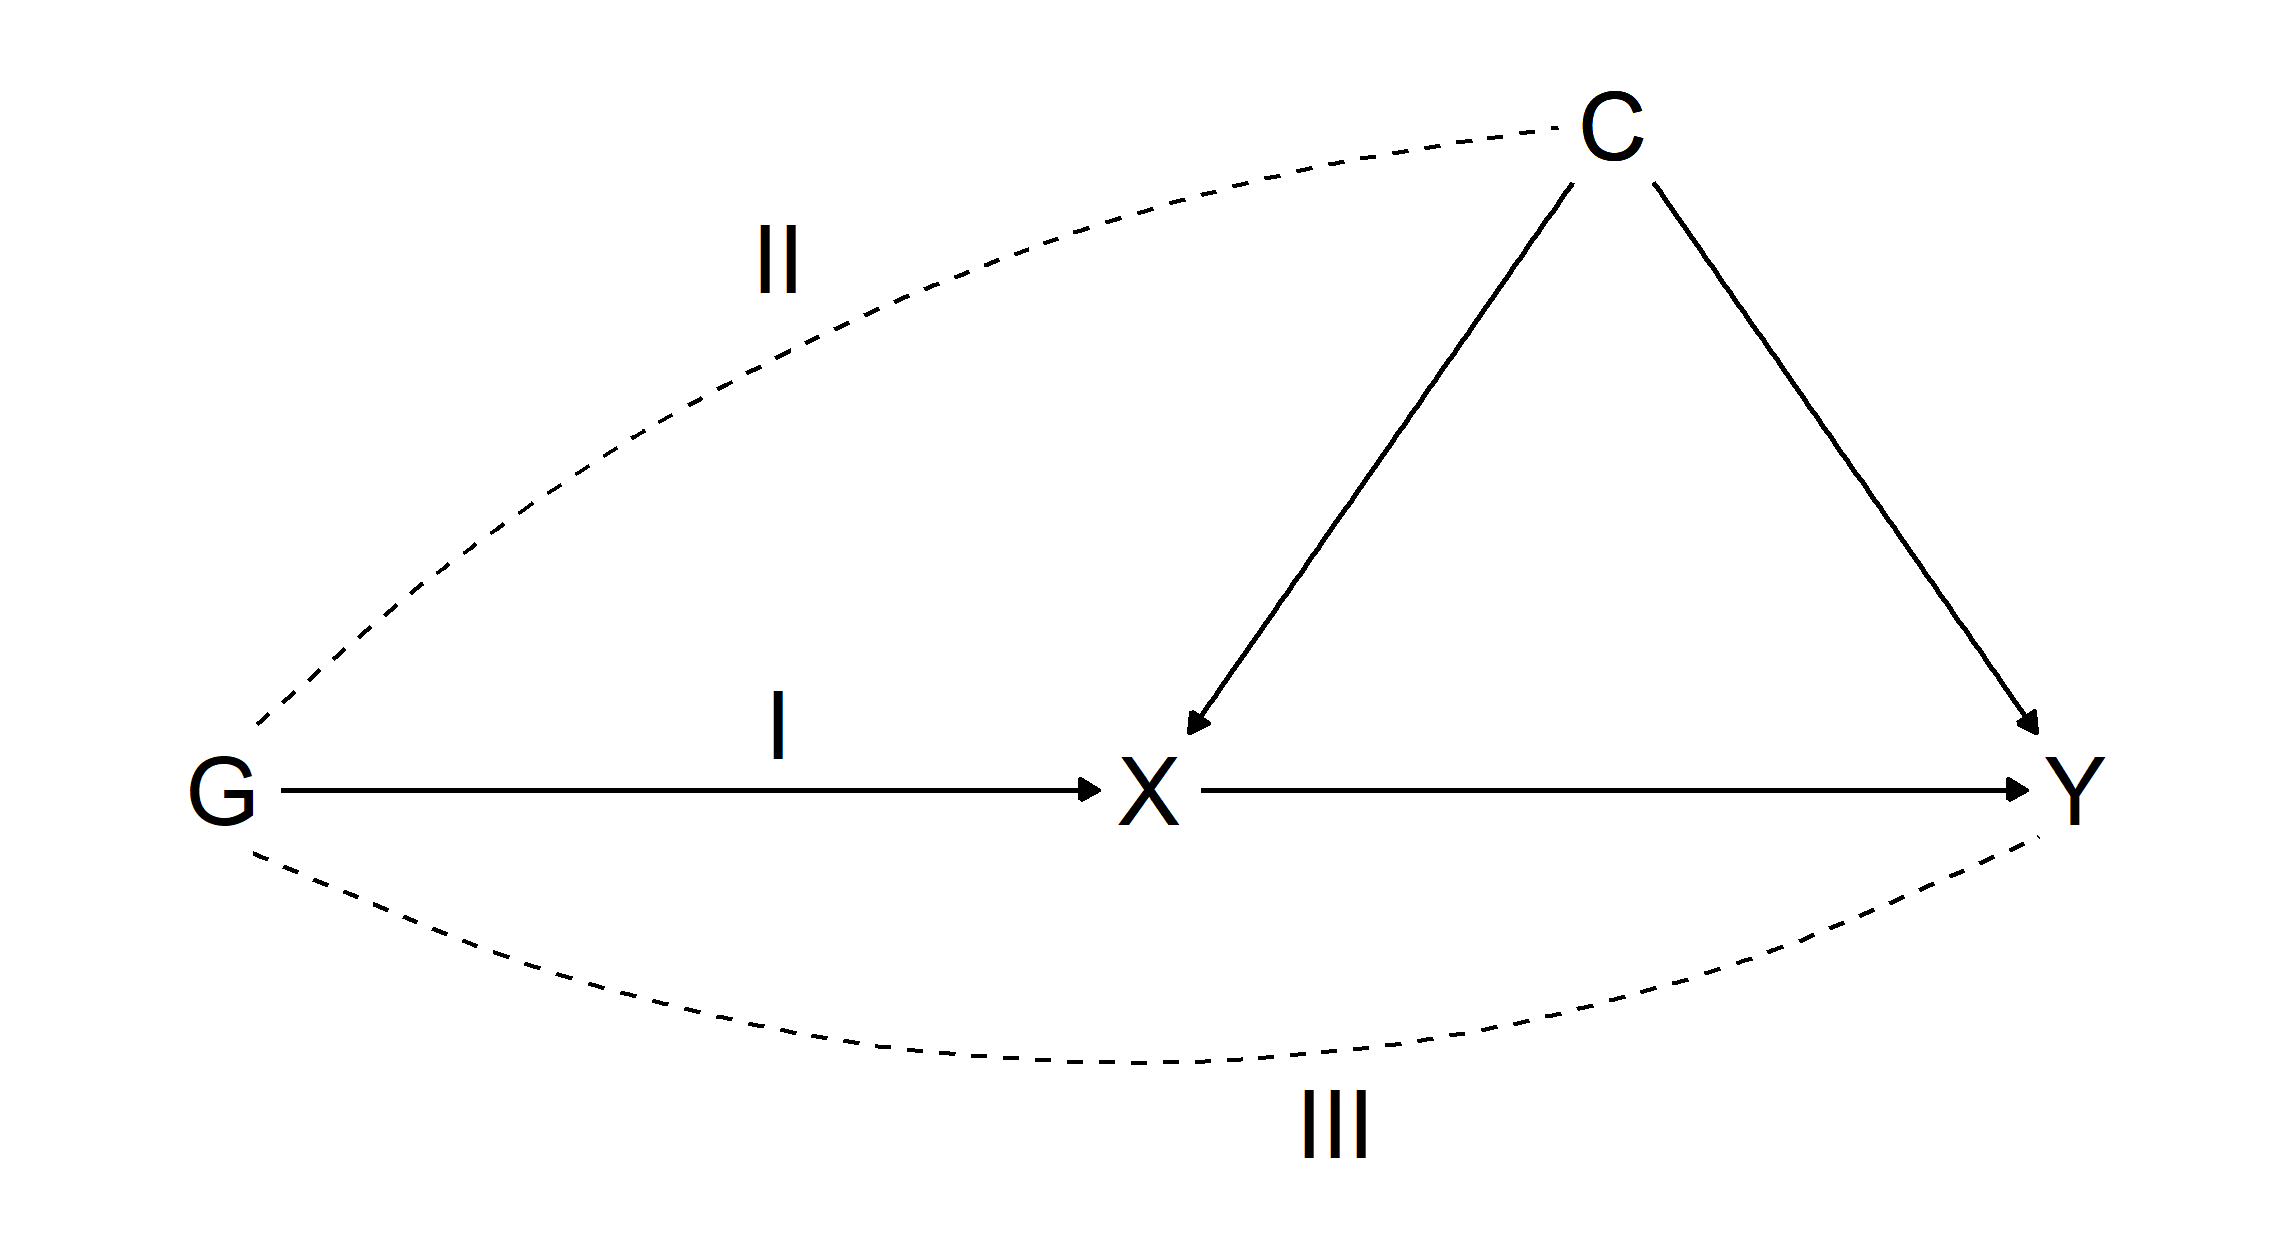
\includegraphics[width=0.7\linewidth]{figures/sys-rev/mrAssumptions} 

}

\caption[Overview of assumptions in Mendelian randomisation analyses]{Summary of the assumptions in Mendelian randomisation analyses: (I) \emph{relevance} - the genetic variant associates with the risk factor of interest; (II) \emph{independence} - the variant-exposure association has no unmeasured confounders; and (III) \emph{exclusion restriction} - variants affect the outcome only through their effect on the risk factor of interest (i.e.~there is no horizontal pleiotropy).}\label{fig:mrAssumptions}
\end{figure}

Firstly, this study design is relatively new, particularly when compared to randomised trials or cohort studies. Figure \ref{fig:typeByYear} demonstrates that Mendelian randomisation studies only begin to appear in the evidence base much later than NRSE/NRSI, likely due to the limited availability of large scale GWAS datasets needed for two-sample Mendelian randomisation analyses. As such, the process and tools for systematically assessing this study design are not as well developed. A key example of this is in the absence of validated search filters for Mendelian randomisation studies. This limitation is further complicated by the varying terminology used to describe the method, particularly in the early years of it's application, which led to me including general terms for instrumental variable analyses in my search.

Additionally, there is currently no widely used risk-of-bias assessment tool for Mendelian randomisation studies. While a recent commentary provided a checklist for interpreting Mendelian randomisation studies, this guide includes reporting items in their quality checklist.\textsuperscript{\protect\hyperlink{ref-davies2018}{69}} While reporting quality is an important consideration, as reflected by the recent release of a STROBE\_MR reporting guidelines,\textsuperscript{\protect\hyperlink{ref-skrivankova2021}{266}} it is a separate consideration to internal validity as discussed in Section \ref{risk-of-bias}. Similarly, a previous review of Mendelian randomisation studies used the Q-Genie tool which was validated to assess the quality of genetic association studies in meta-analysis.\textsuperscript{\protect\hyperlink{ref-sohani2015}{267}} While this tool assesses the underlying GWAS used, it does not assess the additional methodological considerations of the Mendelian randomisation analysis itself. For this review, I used the best available author-devised tool, sourced from a recent review of systematic reviews of Mendelian randomisation studies.\textsuperscript{\protect\hyperlink{ref-spiga2021}{164}}

As a further stumbling block, Mendelian randomisation, particularly when using a two-sample summary data design, is a form of analysis that lends itself to multiple exposure-outcome comparisons. This is particularly relevant to the consideration of bias due to missing evidence. As an example, through snowballing and other measures, I identified at least one relevant Mendelian randomisation study that had not been identified by the search strategy.\textsuperscript{\protect\hyperlink{ref-larsson2017}{70}} On review of this paper, the search would not have been expected to find it given the absence of any lipid-related keywords in the title and abstract. The study examined the association between lipid fractions with Alzheimer's disease as one of many risk factors for the condition. Studies such as this can introduce bias into a systematic review, as it is commonly only those risk factors that show a statistically significant result that are reported in the abstract and so are captured by the search. This may bias systematic reviews, including this one, as the analysis of multiple risk factors against a single outcome within a single publication becomes more common. These studies are described as ``unknown unknown's'' in the context of the RoB-ME tool, and are particularly challenging (as opposed to an analysis that was insufficiently reported to be included in the statistical analysis, or the ``known unknown's'').

Useful future work to improve the methodology for inclusion of Mendelian randomisation studies in systematic reviews should involve the development of a validated search filter for this study design.\textsuperscript{\protect\hyperlink{ref-waffenschmidt2020}{268},\protect\hyperlink{ref-wagner2020}{269}} Alternatively, in better-resourced reviews, a dedicated search for ``risk factors'' and ``dementia'' and ``Mendelian randomisation'' followed by manual review of studies that look across multiple risk factors would be advisable. This was not feasible in the context of this review, given the large number of records to be screened even when using study design filters (n=16,109). Additionally, the value of methods that supporting the traditional bibliographic database search, such as snowballing (forwards and backwards citation chasing) and communication with relevant topic experts should not be underestimated. Finally, development of a risk-of-bias assessment tool for this study design by a panel of methodologists and analysts would be of substantial benefit to the field.

One item of particular interest is the attenuation of any effects observed by Mendelian randomisation studies following the adjustment for/exclusion of genetic variation in the Apoe4 gene region. As covered in the introduction (see Section \ref{intro-basic-science}), an increasing number of ApoE4 alleles is a major independent risk factor for Alzheimer's disease, and so violates the exclusion restriction criteria (Figure \ref{fig:mrAssumptions}). In all cases, excluding these variants attenuates the observed effect to the null. A clear example of this is Benn \emph{et al} (2017), where the ApoE variants were not sufficient identified and excluded and the published paper detailed evidence for a protective effect of LDL-c was identified (RR: 0.83, 95\%CI: 0.75-0.92).\textsuperscript{\protect\hyperlink{ref-benn2017}{73}} Following several rapid responses, the data was re-analysed excluding a larger area around ApoE4 which attenuated the finding to the null.\textsuperscript{\protect\hyperlink{ref-benn2017comment}{270}}

~

\hypertarget{inclusion-of-preprints}{%
\subsection{Inclusion of preprints}\label{inclusion-of-preprints}}

As highlighted in Section \ref{diverse-sources-preprints}, this review explicitly sought to synthesize evidence across different publication statuses (preprinted vs.~published). Using the tool described in Chapter \ref{sys-rev-tools-intro}, two preprint servers related to health and biomedical sciences were searched as part of this review. The small number of studies returned by the searches (or the absence of any relevant hits in the medRxiv database - see Figure \ref{fig:prisma-flow-fig}) is due to the timing of the preprint searches. The searches for this review were performed in mid-July 2019, but the medRxiv repository, an offshoot of the Epidemiology and Clinical Trials categories of the bioRxiv preprint server, only registered its first preprint 25th June 2019. As such, at the point it was searched, the medRxiv database contained only a very small number of records (n=148).





\begin{figure}[H]

{\centering 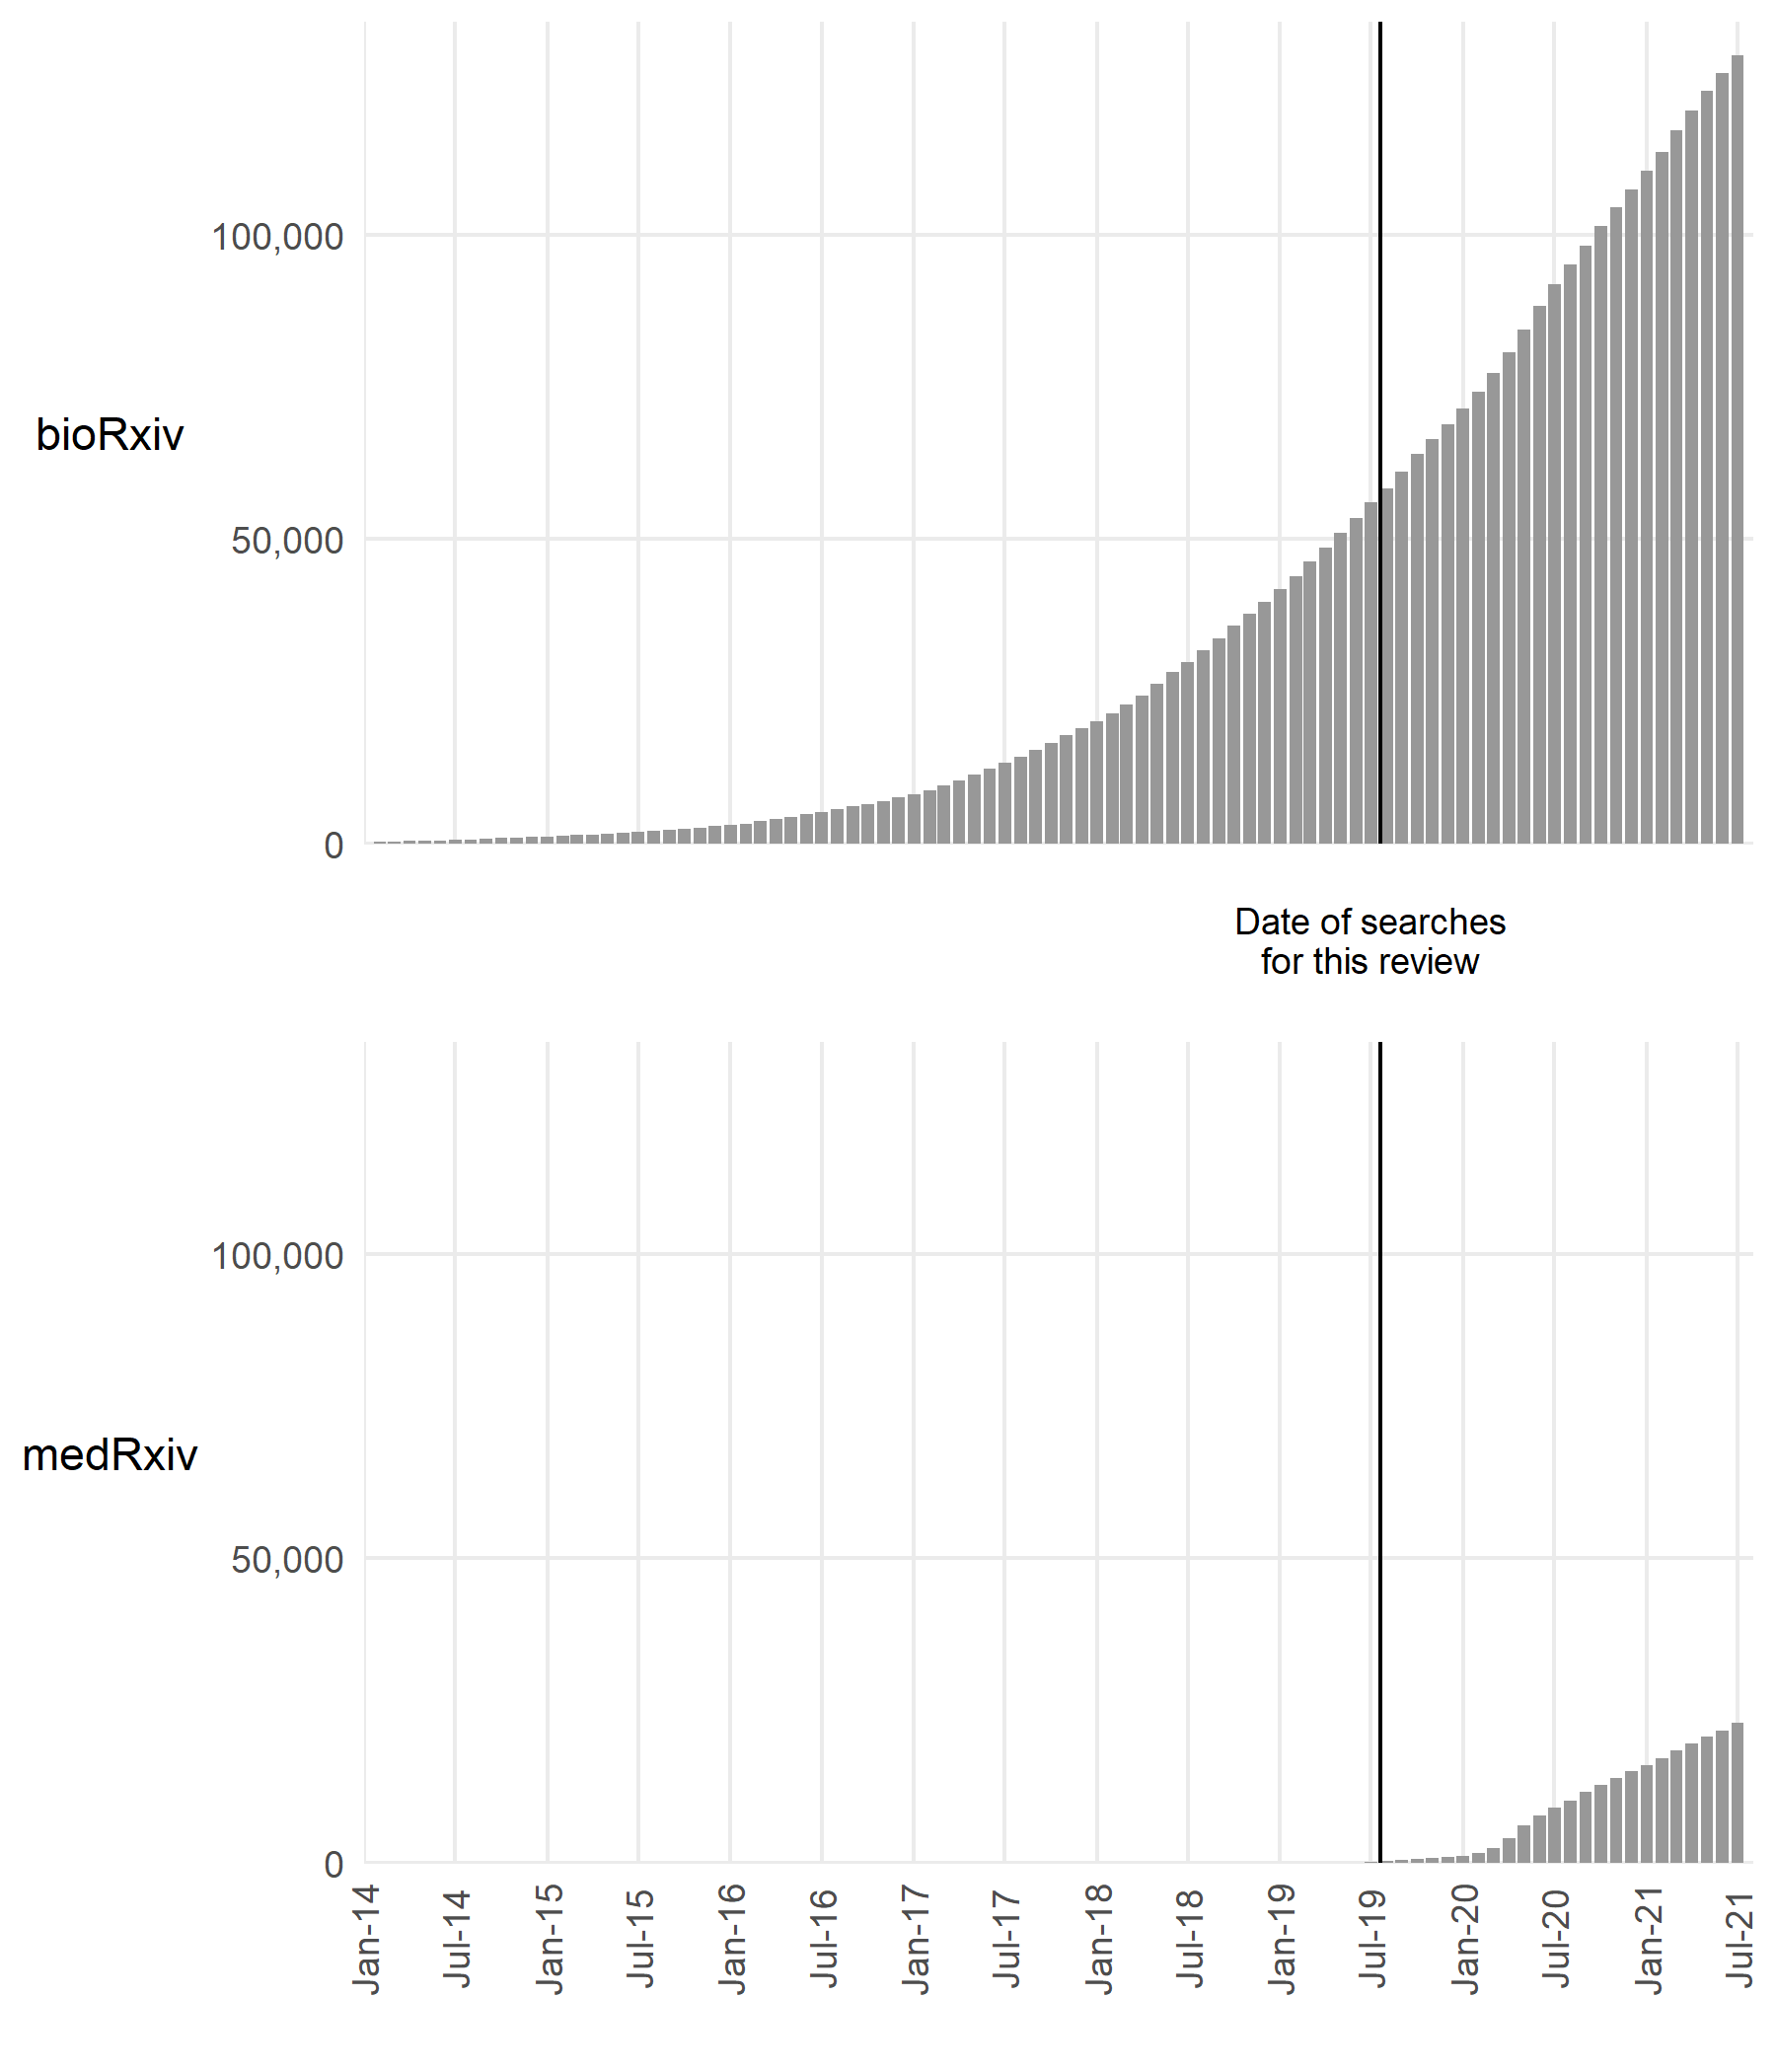
\includegraphics[width=0.8\linewidth]{figures/sys-rev/preprint_growth} 

}

\caption[Growth of preprint repositories over time]{Growth of preprint repositories over time. Given the relative sizes of the preprint repositories at the time the searches for this review were conducted (bioRxiv n= 56,007, medRxiv n = 148), the number of hits returned by each is expected.}\label{fig:preprintGrowth}
\end{figure}

Three relevant preprints from the bioRxiv hits were identified. Of note, all three described Mendelian randomisation studies, potentially indicating that more biologically focused study designs are over-represented in the bioRxiv repository. The added evidential value of including these preprints was described in Section \ref{sys-rev-including-preprints-res} and indicated that results available only via preprinted reports can contribute additional evidence to a meta-analysis. However, the scale of this contribution is questionable. Preprinted evidence was incorporated into only single meta-analysis, and in this case, inclusion of the preprint did not substantially impact the result.

Of the three identified preprints, two were subsequently published as of September 2021. This fits well with the analysis presented in Chapter \ref{sys-rev-tools-heading} that, allowing for a two-year lag, approximately two-thirds of preprints are published, and also illustrates the dual advantages of preprinted reports to evidence syntheses.

Firstly, preprints provide an advance snapshot of the literature, capturing articles that will eventually be published but were not available at the time of the main search. Consider the example of one eligible preprint in this review was initially posted on bioRxiv in July 2019\textsuperscript{\protect\hyperlink{ref-andrews2019}{252}} and was subsequently published in 2021 following peer-review.\textsuperscript{\protect\hyperlink{ref-andrews2021}{247}} Secondly, inclusion of preprints allows for results that may never be formally published to be included in an evidence synthesis exercise as is the case with the second preprint included in this review.\textsuperscript{\protect\hyperlink{ref-so2017}{250}} Both of these aspects illustrate that, if the aim is to find the current state of the art in the topic area at the time of searching, inclusion of preprints is a necessity.

More recently, inclusion of preprints in systematic reviews has become significantly more widespread. This is largely due to the role of preprint servers, in particular medRxiv, as a key evidence dissemination venue during the early stages of the COVID-19 pandemic.\textsuperscript{\protect\hyperlink{ref-fraser2020preprinting}{82}} How well this adoption of preprints will transfer to other less-urgent topics, where the speed of research does not put the same focus on preprinted articles, is currently unknown.

~

~

\hypertarget{sys-rev-open-data}{%
\subsection{Open data sharing}\label{sys-rev-open-data}}

As discussed in Section \ref{dose-response-results}, many primary studies did not report important information required for the dose-response meta-analysis, and so could not be included in the synthesis. This limitation was compounded by the expected low response rate to requests for further information from primary authors. While contacting authors is worthwhile, as it can substantially change the conclusion of a systematic review\textsuperscript{\protect\hyperlink{ref-meursingereynders2019}{271}} and is not too costly to systematic reviewers,\textsuperscript{\protect\hyperlink{ref-cooper2019}{272}} a far preferable option is that the authors of primary studies readily deposit all relevant study data at the point of publication.

Based on my experience of extracting data for this review, I co-authored a guidance article to aid primary prevention scientists in preparing and sharing their data so that it can easily be incorporated into a evidence synthesis exercise, using a trial of mindfulness interventions as an case study.\textsuperscript{\protect\hyperlink{ref-hennessy2021}{273}} A copy of this publication is available in Appendix \ref{published-papers}. In an attempt to apply my own guidance, I have invested a substantial amount of time and effort into making the data obtained by this review openly available to other researchers.

~

\hypertarget{strengths-and-limitations}{%
\subsection{Strengths and limitations}\label{strengths-and-limitations}}

\hypertarget{strengths}{%
\subsubsection{Strengths}\label{strengths}}

I believe there are several aspects where this review is distinct from those reviews already available in the published literature. While several reviews of this research topic exist,\textsuperscript{\protect\hyperlink{ref-chu2018}{257}--\protect\hyperlink{ref-poly2020}{260}} the overlap between the list of studies included in each is not 100\%. As part of this review, I have not only performed a original search of primary literature databases, but have also screened the reference lists of comparable reviews to ensure no study has been omitted. In addition, this review employed a structured approach to risk-of-bias assessment using a domain-based tool. This represents an important strength of this review, as the detailed risk of bias assessments are used in inform the quantiative triangulation analysis presented in Chapter \ref{tri-analysis-heading}.

Thirdly, as discussed at length in the section above, in contrast to other available reviews and enabled by the tool described in Chapter \ref{sys-rev-tools-heading}, this review systematically searched preprinted health-related preprints. Finally, as a secondary element, I used this review to pilot new research synthesis methodologies, in particular a new visualisation approach for risk-of-bias assessments and a forthcoming tool for assessing the risk-of-bias due to missing evidence.

~

\hypertarget{limitations}{%
\subsubsection{Limitations}\label{limitations}}

The primary limitation of this review is that several included studies used data from EHR databases, which come with serious concerns regarding validity\textsuperscript{\protect\hyperlink{ref-hsieh2019}{274}} \textsuperscript{\protect\hyperlink{ref-mcguinness2019validity}{275},\protect\hyperlink{ref-wilkinson2018}{276}} Relatedly, several studies which made use of electronic health record database did not report the specific code lists used, potentially introducing substantial heterogeneity between effect estimates. An empirical example of the effect of differing EHR code list is presented as part of the analysis in Chapter \ref{cprd-analysis-heading} (see Section \ref{comparing-codelists}).

In addition, the fact that only a sample of records were dual screened at the title/abstract and full-text stages is a potential limitation, as there is a chance that some eligible records could have been excluded. However, evidence from assessments of inter- and intra-rater reliability indicate that is not a major concern.

One particular limitation with regards to the risk-of-bias assessment is the fact that the ROBINS-E assessments were performed without the tool being finalised. This meant that there were no signaling questions to guide the domain-level risk-of-bias assessment, which may have influenced the accuracy with which domain-level judgements were assigned. However, there is no published empirical evidence supporting the need for signaling questions, and assessment of inter-rater reliability across the different tools did not indicate a specific problem with the ROBINS-E assessments. In fact, low agreement was common across the tools, though this is expected based on the available literature.\textsuperscript{\protect\hyperlink{ref-jeyaraman2020}{277}}

One further limitation is the fact that the risk of bias due to missing evidence assessment, combined with some empirical evidence that some studies were missed by the search but contained relevant studies is a definite limitation of this review (see Section @Ref(rev-discussion-MR) above for a fuller discussion of this issue with respect to Mendelian randomisation studies). Unfortunately, this is probably a common limitation across all reviews, based on the way in which increased search sensitivity must be balanced with a reasonable workload.

~

\hypertarget{summary-3}{%
\section{Summary}\label{summary-3}}

\begin{itemize}
\item
  In this chapter, I presented the results of a comprehensive systematic review of existing evidence on the association between lipid levels and dementia use. The review included both direct (studies that examined lipid levels directly) and indirect (studies examining lipid-lowering via treatments such as statins) forms of evidence. In contrast to previous reviews, I also included preprinted evidence, facilitated by the research tool introduced in Chapter \ref{sys-rev-tools-heading}.
\item
  I found no consistent relationship across different evidence sources, though there was some indication of a protective effect of statins on all-cause and Alzheimer's disease dementia in non-randomised studies of interventions.
\item
  The findings from this review are used though out the subsequent chapters: in Chapter \ref{cprd-analysis-heading}, summary of the evidence guided the choice of analysis approach, ensuring that the new analysis was at risk of a different source of bias and provided evidence on an under-studied outcome (vascular dementia); while in Chapter \ref{ipd-heading}, prospective cohorts identified by the review were contacted in an attempt to obtain individual participant data ; finally, the results identified here are used as a key source of evidence for the triangulation exercise presented in Chapter \ref(discussion-heading).
\end{itemize}

\newpage

\hypertarget{references-3}{%
\section{References}\label{references-3}}

\begin{savequote}
When dealing with human beings controlled experiments frequently prove
to be impracticable, so for a scientific basis for our assumptions we
turn to past history to reconstruct the suspected causal chain of events
- and then our statistical troubles may begin.
\qauthor{--- Harold F. Dorn, 1953\textsuperscript{\protect\hyperlink{ref-dorn1953}{278}}}\end{savequote}



\hypertarget{cprd-analysis-heading}{%
\chapter{Primary analysis of lipid-regulating agents and dementia outcomes}\label{cprd-analysis-heading}}

\minitoc 

\hypertarget{lay-summary-4}{%
\section{Lay summary}\label{lay-summary-4}}

Electronic health record (EHR) databases are large collections of medical data, used to manage patient administration and care. Under these systems, whenever a patient attends their GP, their clinical data is recorded in a central database using a standardised coding system. These databases have several advantages over traditional methods of data collection, including the number of people they contain and the relatively low cost of data collection via routine care. This is particularly important when studying diseases such as dementia, which may begin to develop in patients long before symptoms are seen.

This analysis makes use of the Clinical Practice Research Datalink (CPRD), which contains the electronic medical records of more than 3 million people from general practices across England. Using this data, the analysis presented in this chapter examined whether treatments which lower cholesterol levels (also known as lipid-regulating agents or LRA) of which statins are a prime example, affect the risk of all-cause dementia and related outcomes (Alzheimer's disease, vascular dementia and other dementias).

Little evidence for an effect of lipid-regulating agents effect on the risk of Alzheimer's disease was found, with the exception of a slightly increased risk in those prescribed a certain type of lipid-regulating agent called fibrates. In contrast, I found an increased risk of vascular and other (i.e.~non-Alzheimer's) dementia was associated with lipid-regulating agent use.

This increased risk in outcomes with a vascular element (e.g.~vascular dementia) is unexpected, and is very likely to be due to the presence of bias in the analysis. This bias, called ``confounding by indication'', is caused when those who are prescribed a statin are more at risk of vascular dementia for a range of reasons, which makes it appear as if statins are harmful. Despite this limitation, the analysis presented provides an important source of information which will be used in later chapters.

~

\hypertarget{introduction-2}{%
\section{Introduction}\label{introduction-2}}

In this Chapter, I present an analysis of a large population-based electronic health record dataset to investigate the relationship between lipid-regulating agent (LRA) use and dementia outcomes. The analysis aims to address important two limitations of the current evidence base as identified by the systematic review presented in Chapter \ref{sis-rev-heading}.

Firstly, it explicitly examines vascular dementia as an outcome. The systematic review presented in the previous chapter identified an evidence gap around the effect of lipid-regulating agents on the risk of vascular dementia. As triangulation exercises require as many diverse sources of evidence as possible, this analysis provides a source of information on this outcome.

Secondly, and in a similar vein, the analysis intentionally takes a different analytical approach to that most commonly used to examine the effect of statins on dementia as identified by the systematic review. Specifically, this involved a concerted effort to address immortal time bias though use of a Cox proportional hazards analysis, incorporating a time-varying treatment indicator.\textsuperscript{\protect\hyperlink{ref-suissa2008}{279}} By employing this approach, the analysis provides an evidence source at risk of a distinct bias. The results from this analysis will be incorporated into the triangulation exercise presented in Chapter \ref{discussion-heading}.

This chapter represents an extended version of a preprint manuscript, a copy of which is available in Appendix \ref{published-papers}.

~

\hypertarget{methods-1}{%
\section{Methods}\label{methods-1}}

\hypertarget{study-protocol}{%
\subsection{Study protocol}\label{study-protocol}}

An \emph{a priori} protocol for this study was published,\textsuperscript{\protect\hyperlink{ref-walker2016}{280}} and amendments to this are recorded in Appendix \ref{appendix-cprd-amendments}.\textsuperscript{\protect\hyperlink{ref-vonelm2008}{281}}

~

\hypertarget{cprd-data-source}{%
\subsection{Data source}\label{cprd-data-source}}

Previously known as the General Practice Research Database (GPRD), the Clinical Practice Research Datalink (CPRD) is a large population-based electronic health record (EHR) database.\textsuperscript{\protect\hyperlink{ref-herrett2015}{282}} The database has been collecting primary care data from participating practices across England since 1987.\textsuperscript{\protect\hyperlink{ref-williams2012}{283},\protect\hyperlink{ref-wood2001revitalizing}{284}} It contains the primary care records for more than 10 million primary care patients in England, and is broadly representative of the UK population in terms of age, sex and ethnicity.\textsuperscript{\protect\hyperlink{ref-herrett2015}{282},\protect\hyperlink{ref-mathur2014}{285}}

To avoid the ambiguity of interpreting free-text clinical notes and to allow for easy analysis of the resulting data, the CPRD primarily collects data using a predefined coding system known as Read codes.\textsuperscript{\protect\hyperlink{ref-booth1994}{286}} All clinical events, included clinical test results and diagnoses, can be identified by a specific Read code. The codes use a nested approach (see Table \ref{tab:readExample-table}), with the initial characters defining broad diagnostic topics (e.g.~Eu\ldots{} - Mental and behavioural disorders), while subsequent characters provide additional information on the specific condition diagnosed (e.g.~Eu001 - Dementia in Alzheimer's disease with late onset).

~





\begin{table}[H]

\caption[Example of CPRD Read code hierarchy]{\label{tab:readExample-table}Example of CPRD Read code hierarchy, showing how ``Dementia in Alzheimer's disease with late onset'' (\emph{Eu001}) is nested under the top-level of ``Mental disorders'' (\emph{Eu\ldots{}}). Broad topics are specified using the initial two alpha-numeric characters of the Read code, while subsequent characters are used to define specific conditions and context.}
\centering
\begin{tabular}[t]{cll}
\toprule
\textbf{Level} & \textbf{Read code} & \textbf{Term}\\
\midrule
1 & E.... & Mental disorders\\
2 & Eu... & Mental and behavioral disorders\\
3 & Eu0.. & Organic mental disorder\\
4 & Eu00. & Dementia in Alzheimer's disease\\
5 & Eu001 & Dementia in Alzheimer's disease with late onset\\
\bottomrule
\end{tabular}
\end{table}

~

The index events, exposures and outcomes used in this analysis were identified using predetermined code lists, which are available for inspection from the archived repository accompanying this analysis (data/code availability is discussed in Section \ref{cprd-data-avail}).

~

\hypertarget{cohort-definition}{%
\subsection{Cohort definition}\label{cohort-definition}}

This analysis included all participants registered at a participating practice between 1 January 1995 and 29 February 2016 who had a flag for ``research quality'' data (as defined by the CPRD). Records pre-dating the 1995 cut-off were included in the original CPRD extract obtained for this analysis. However, these were excluded from the analysis as data quality and reliability are thought to be higher after this date.\textsuperscript{\protect\hyperlink{ref-wolf2019}{287}} Additionally, individuals with less than 12 months of continuous records prior to cohort entry were excluded, making the effective start date of the cohort 1 January 1996.

Participants were included in the study cohort if their record contained any of the following index events: a Read code for a diagnosis of hypercholesterolemia or related condition; a Read code for prescription of a lipid-regulating agent (such as statins); a total cholesterol test result of \textgreater4 mmol/L; or an LDL-c test result of \textgreater2 mmol/L.\textsuperscript{\protect\hyperlink{ref-walker2016}{280}} The blood lipid cut-offs were based on NIHR-recommended levels at the time the protocol was written. These index events allowed me to define a population of participants who were either at risk of hypercholesterolemia, as indicated by the elevated total or LDL cholesterol test results, or had already been diagnosed with it, as indicated by a diagnostic code/related prescription.

The index date for a participant was defined as the date where the first relevant code or test result was recorded on their clinical record, and participants were followed up until the earliest of: (a) an outcome of interest; (b) death; (c) end of follow-up (29 February 2016); (d) last registration date with their GP practice; or (e) the last CPRD collection date for their practice. Participants were ineligible for our cohort if they were less than 40 years of age (as these patients are less likely to be prescribed a LRA), had less than 12 months of ``research quality'' data, were simultaneously prescribed more than one lipid-regulating agent (due to the difficult of assigning these to a single exposure group), or were diagnosed with an outcome of interest before or on the date of the index event (i.e.~had less than one full day of follow-up).

~

\hypertarget{exposures}{%
\subsection{Exposures}\label{exposures}}

I considered seven lipid-regulating drug classes based on groupings in the British National Formulary (BNF),\textsuperscript{\protect\hyperlink{ref-wishart2017}{288}} namely: statins, fibrates, bile acid sequestrants, ezetimibe, nicotinic acid groups, ezetimibe and statin (representing one treatment containing both drugs, rather than the two classes being prescribed concurrently), and omega-3 fatty acid groups.

A participants drug class was assigned based on their first recorded prescription, and any drug switching was ignored in an effort to mimic an intention-to-treat approach. We did however examine how often the initial drug class altered according to one of three criteria:

\begin{itemize}
\tightlist
\item
  \textbf{stopped}: defined as the last prescription of the primary class being followed by at least six months of observation;
\item
  \textbf{added}: defined as a second drug class being prescribed before the last prescription of the initial class; and
\item
  \textbf{switched}: defined as a second drug class being prescribed after the last prescription of the initial class.
\end{itemize}

~

\hypertarget{cprd-outcomes}{%
\subsection{Outcomes}\label{cprd-outcomes}}

I considered five outcomes as part of this analysis: probable Alzheimer's disease, possible Alzheimer's disease, vascular dementia, other dementias, and a composite all-cause dementia outcome. When two or more outcomes were coded in a participant's clinical record, a decision tree was used to differentiate between them (Figure \ref{fig:decisionTreeFig}). The diagnosis date of the outcome was determined by the first record of a relevant code.





\begin{figure}[H]
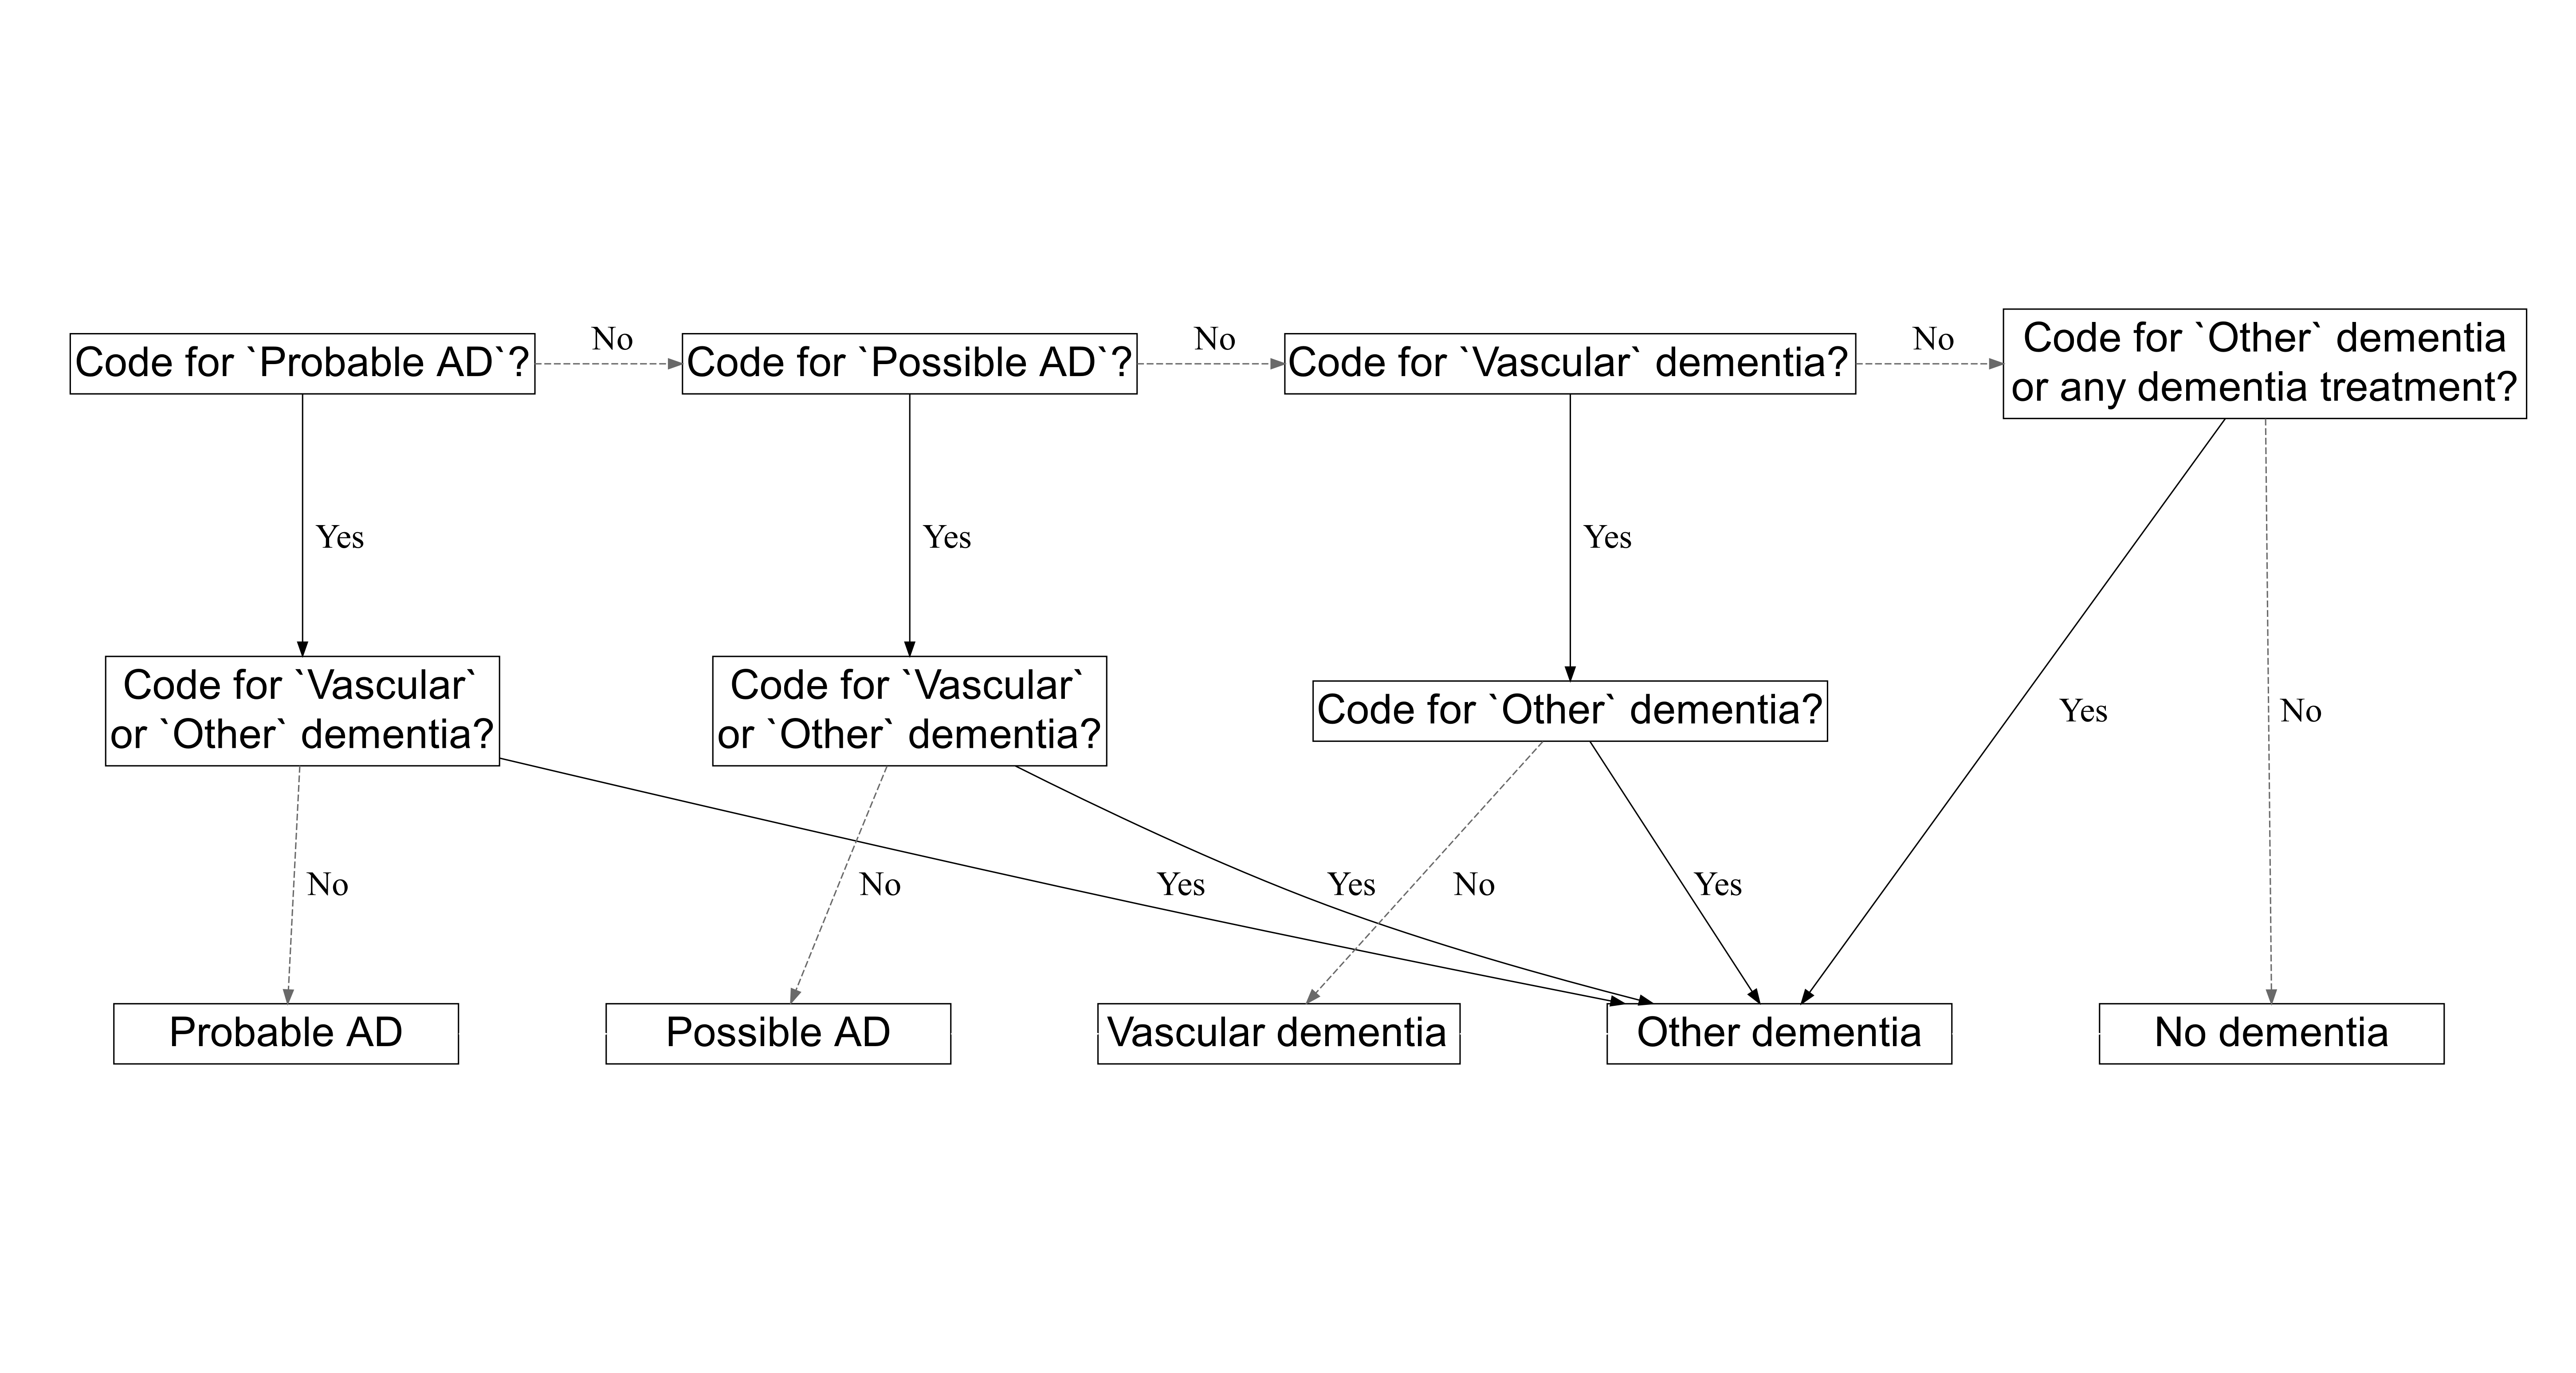
\includegraphics[width=1\linewidth]{figures/cprd-analysis/decision_tree} \caption[Decision tree for assigning dementia subtypes]{Decision tree for assigning dementia subtypes, based on the presence of Read codes in the patient's record. Note that an outcome of ``probable'' or ``Possible'' Alzheimer's disease (AD) requires the absence of any vascular outcome codes.}\label{fig:decisionTreeFig}
\end{figure}

~

\hypertarget{covariates}{%
\subsection{Covariates}\label{covariates}}

A range of additional variables were included in the analysis, intended to address the different distributions of potential confounding variables between those who were prescribed an lipid-regulating agent and those who were not. These are discussed in detail below and summarised in Table \ref{tab:covariateDef-table}.

~









Charlson index implemented using Read code lists.\textsuperscript{\protect\hyperlink{ref-khan2010}{290}} Code lists based on those by Taylor et al.\textsuperscript{\protect\hyperlink{ref-taylor2016}{291}}

\begin{table}[H]

\caption[Covariates adjusted for.]{\label{tab:covariateDef-table}Definition of covariates adjusted for in the full-adjusted model. The code lists used to define the majority of these covariates were originally created for use in a previously published analysis.\textsuperscript{\protect\hyperlink{ref-walker2020}{289}} while others were built on or adapted from previous published work,\textsuperscript{\protect\hyperlink{ref-khan2010}{290}--\protect\hyperlink{ref-wright2017}{292}}.}
\centering
\fontsize{9}{11}\selectfont
\begin{tabular}[t]{>{\raggedright\arraybackslash}p{15em}>{\centering\arraybackslash}p{25em}}
\toprule
\textbf{Covariate } & \textbf{How was the covariate defined?}\\
\midrule
Previous history of coronary arterial disease & Presence of one or more relevant Read codes on record.\\
\midrule
Previous history of coronary bypass surgery & Presence of one or more relevant Read codes on record.\\
\midrule
Previous history of cerebrovascular disease (including stroke) & Presence of one or more relevant Read codes on record.\\
\midrule
Chronic illness, including cancer and arthritis & Charlson index implemented using Read code lists.\textsuperscript{\protect\hyperlink{ref-khan2010}{290}} Code lists based on those by Taylor et al.\textsuperscript{\protect\hyperlink{ref-taylor2016}{291}}\\
\midrule
Socioeconomic position & 2010 English Index of Multiple Deprivation (IMD) at the twentile level, where 1 represents the least deprived and 20 the most deprived.\\
\midrule
\addlinespace
Consultation rate & Calculated by dividing the total number of clinic visits by the length of the patient record prior to the index date to give an average annual rate.\\
\midrule
Alcohol status & Recorded value (current, former or never).\\
\midrule
Smoking status & Most recent of recorded value (current, former or never) or Read code indicating a recorded value. Code lists based on those by Wright et al.\textsuperscript{\protect\hyperlink{ref-wright2017}{292}}\\
\midrule
Body Mass Index & Recorded value if available, or a calculated value using the last recorded height and weight measurements. Measurements taken before the age of 25 were excluded to ensure adult measurements were used.\\
\midrule
Peripheral arterial disease & Presence of one or more relevant Read codes on record.\\
\midrule
\addlinespace
Hypertension & Presence of one or more relevant Read codes on record.\\
\midrule
Baseline total cholesterol & Continuous value recorded as test result ("enttype==163 \& test\_data1==3")\\
\midrule
Baseline LDL cholesterol & Continuous value recorded as test result ("enttype==177 \& test\_data1==3")\\
\midrule
Chronic kidney disease & Presence of one or more relevant Read codes on record.\\
\midrule
Type 1 Diabetes & Presence of one or more relevant Read codes on record.\\
\midrule
\addlinespace
Type 2 Diabetes & Presence of one or more relevant Read codes on record.\\
\bottomrule
\end{tabular}
\end{table}

~

Demographic covariates adjusted for included age and gender. Age in years was calculated at date of entry into the cohort, using the 1st of January of a patients' birth year (the exact date of birth was not provided by CPRD), and was adjusted for via its use as the time axis for the Cox model (see Section \ref{cprd-time-axis}). Socioeconomic status was proxied using the Index of Multiple Deprivation (IMD) 2010, which draws on seven domains (income; employment; education, skills and training; health and disability; crime; barriers to housing and services; living environment) to create an overall deprivation score for each of 32844 statistical geography areas in England. To help preserve patient privacy, IMD score is only available from the CPRD in twentiles, with 1 indicating the least deprived and 20 indicating the most deprived. Smoking and alcohol use was determined at index, and participants were categorised as current, former, or never users of each.

Body mass index (a summary measure calculated as \(weight/height^2\)), baseline total cholesterol and baseline LDL cholesterol measures were obtained, using the last recorded value prior to the index date. A variable indicating grouped year of entry into the cohort (\textless=2000, 2001-2005, 2006-2010, \textgreater2010) was included to allow for changes in prescribing trends across the lifetime of the cohort. To assess healthcare utilisation, I adjusted for the average annual number of consultations between the beginning of a patients data and their entry into the cohort.

Finally, presence of a range of related conditions at baseline were accounted for, including cardiovascular disease, coronary bypass surgery, coronary artery disease, peripheral arterial disease, hypertension, chronic kidney disease, and Type 1 and Type 2 diabetes. In addition to adjusting for these covariates individually, a Charlson co-morbidity index (CCI) score was calculated for each participant. The CCI is a weighted index that uses presence and severity of a number of conditions to enable adjustment for the general health of a participant in terms of their mortality risk.\textsuperscript{\protect\hyperlink{ref-charlson1987new}{293}} The conditions considered under the index are: AIDS; cancer; cerebrovascular disease; chronic pulmonary disease; congestive heart disease; dementia; diabetes; diabetes with complications; hemiplegia; metastatic tumour; mild liver disease; moderate liver disease; myocardial infarction; peptic ulcer disease; peripheral vascular disease; renal disease; and rheumatological disease. Inclusion of this index allowed me to attempt to adjust for the general health of patients included in the analysis.

code lists for all covariates can be found in the archived data repository accompanying this analysis (see Section \ref{cprd-data-avail}).

~

\hypertarget{missing-data}{%
\subsection{Missing data}\label{missing-data}}

Missing data are a recognised issue in electronic health records databases,\textsuperscript{\protect\hyperlink{ref-wells2013strategies}{294}} given that they contain administrative data, collected primarily for the purposes of patient management and care rather than academic research.

In this analysis, missing data were handled using a multiple imputation approach.\textsuperscript{\protect\hyperlink{ref-sterne2009}{295}} Variables with missing observations were identified for inclusion in the imputation model. Nominal variables with missing values were modelled using multinomial logistic regression, while continuous variables were modelled using linear regression. As per best practice, all variables used in the analytic model, including the outcome, were included in the imputation model.\textsuperscript{\protect\hyperlink{ref-moons2006}{296}} Using the MICE (Multiple Imputation by Chained Equations) command in STATA16, 20 imputed datasets were created.

Missing data was only considered an issue for variables where a numerical test result was expected (e.g.~BMI), or where a code existed for the absence of the condition (e.g.~categorical smoking status). This approach was necessary, as absence of a code for other treatments or conditions (e.g.~statin use or dementia) was assumed to indicate absence of the treatment/condition rather than being considered missing.\textsuperscript{\protect\hyperlink{ref-wells2013strategies}{294}}

~

\hypertarget{estimation-methods}{%
\subsection{Estimation methods}\label{estimation-methods}}

A Cox proportional hazards (PR) model was used to estimate the effect of statins on dementia outcomes. Cox PR models are defined in general terms as:

\begin{equation}
  h(t) = h_o(t) \times exp(b_1x_1 + b_2x_2 + ... +b_px_p)
  \label{eq:cox-model}
\end{equation}

where:

\begin{itemize}
\tightlist
\item
  \(t\) is the survival time;
\item
  \(h(t)\) is the hazard function; and
\item
  \(x_1,x_2,...,x_p\) are the covariates which determine the hazard function, while \(b_1,b_2,...,b_p\) are the coefficients for each covariate.
\item
  \(h_o(t)\) is the baseline hazard - when all \(x_i\) are zero, the \(exp()\) function resolves to 1.
\end{itemize}

A Cox PR model was chosen for this analysis as it inherently accounts for the length of time participants spend in each exposure group. Using this approach, time-at-risk can be properly attributed to the appropriate exposure group, thus mitigating the impact of immortal time bias. This is discussed in detail in the following section.

~

\hypertarget{cprd-immortal-time-bias}{%
\subsection{Immortal time bias and time-varying treatment indicators}\label{cprd-immortal-time-bias}}

Immortal time bias describes two distinct but related types of bias. The first presentation, the selection bias aspect (Panel A, Figure \ref{fig:immortalTimeBias}), occurs when time prior to the exposure is excluded leading to the exposed and control groups being followed up from different time points.\textsuperscript{\protect\hyperlink{ref-levesque2010}{297}} Following the example displayed in the figure, the unexposed group are followed from the date of a diagnosis, while the exposed group is followed from date of a prescription. In this scenario, the time between diagnosis and prescription for the exposure group is missing, and any events that occur in the exposed group prior to the prescription will be inappropriately excluded from the analysis.

The second presentation of immortal time bias is as a type of misclassification bias (Panel B, Figure \ref{fig:immortalTimeBias}). It occurs when the exposure time prior to the prescription, and any events occurring within it, is inappropriately assigned to the exposed group.

~





\begin{figure}[H]
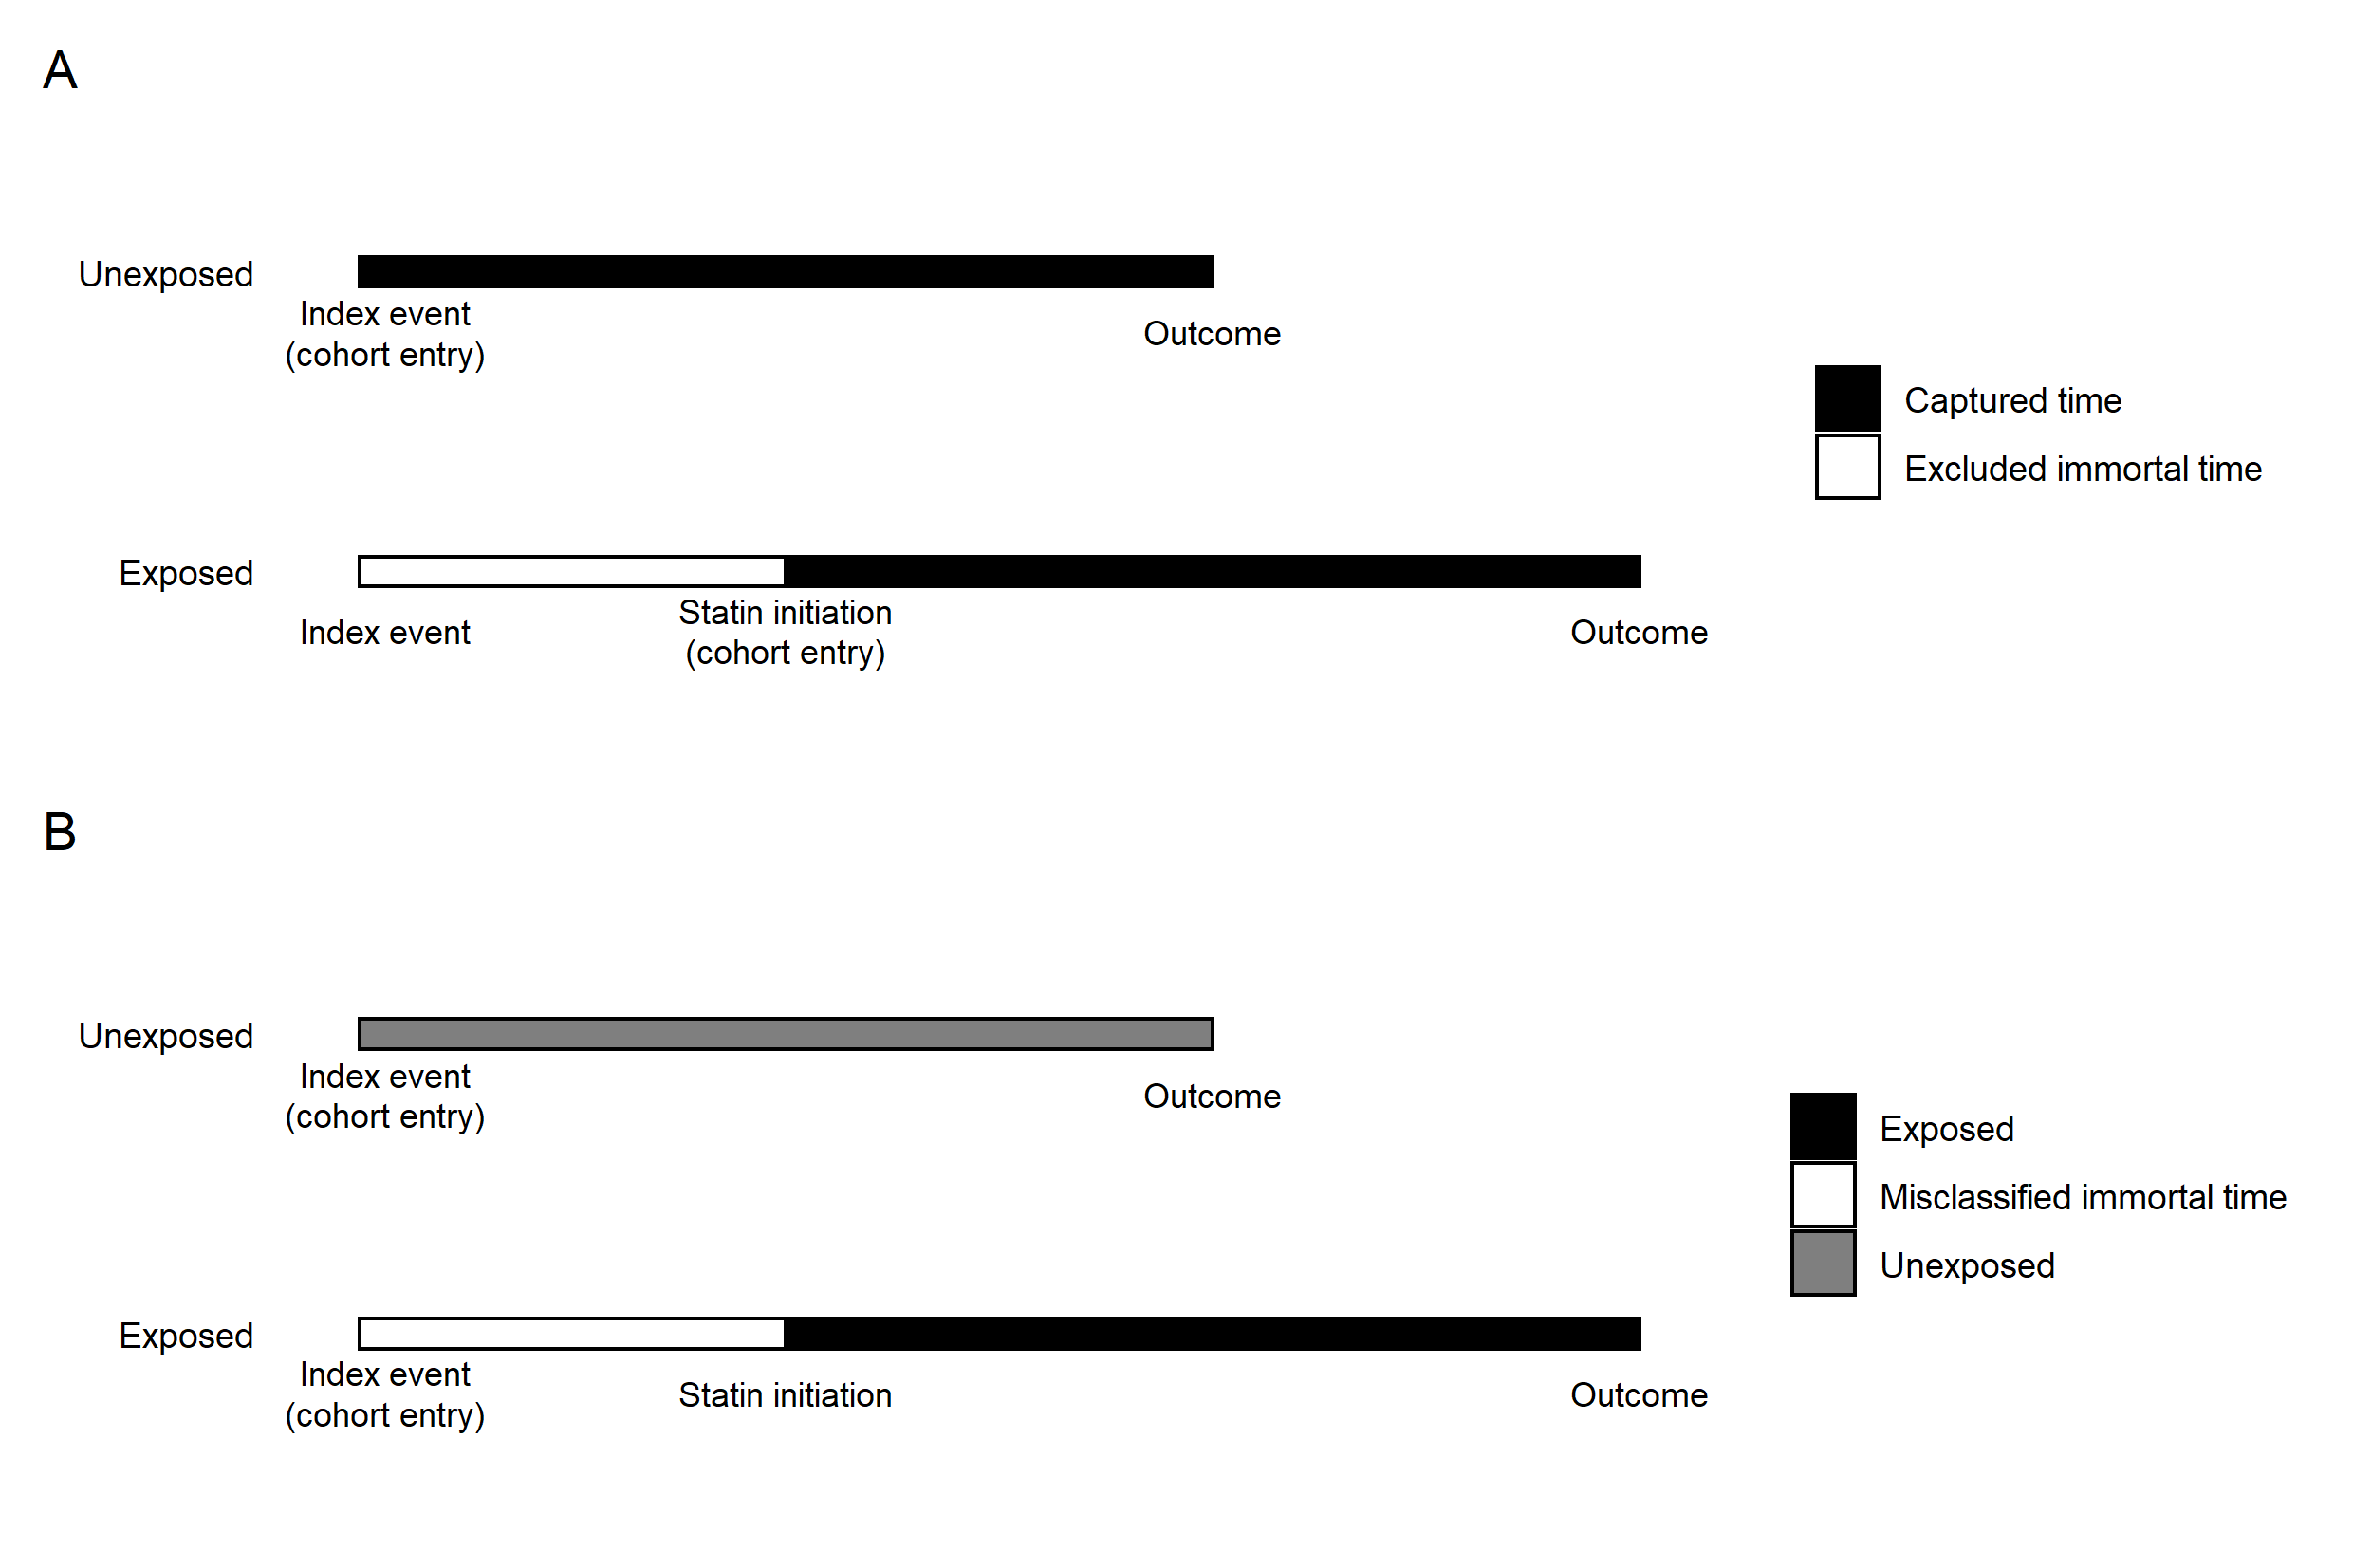
\includegraphics[width=1\linewidth]{figures/cprd-analysis/immortal_time} \caption[shortcap]{Diagram illustrating the two presentations of immortal time bias, as a selection bias (Panel A) and a misclassification bias (Panel B).}\label{fig:immortalTimeBias}
\end{figure}

~

This second presentation appears to be common in the existing literature, as several of the studies included in the systematic review presented in Chapter \ref{sys-rev-heading} were identified as being at risk of immortal time bias following formal risk of bias assessment using the ROBINS-I tool (see Section \ref{risk-of-bias-subheading}). Both presentations of immortal time bias appear in the literature on the relationship of statins and dementia, as identified by the systematic review presented in Chapters \ref{sys-rev-methods-heading}/\ref{sys-rev-results-heading}

This analysis attempted to address this issue by following all participants from a common index date (defined as earliest of: (a) date of raised cholesterol test results; (b) hypercholesterolemia diagnosis; or (c) LRA prescription). Following a recommended approach to addressing the second form of immortal time bias, I employed a time-varying indicator of treatment status to correctly allocate time-at-risk to the exposed and unexposed groups.\textsuperscript{\protect\hyperlink{ref-levesque2010}{297}}

Under this approach, all patients start in the unexposed group and contribute time-at-risk until they are prescribed a lipid-regulating agent and move into the exposed group. Note, patients for whom prescription of a lipid-regulating agent was the index event only contribute time to the exposed group (i.e.~they enter the cohort and move into the exposed group on the same day).

~

\hypertarget{cprd-time-axis}{%
\subsection{Time axis}\label{cprd-time-axis}}

As part of a Cox proportional hazard model, there is the option to use either absolute time in cohort or participants age as the time scale of interest.\textsuperscript{\protect\hyperlink{ref-lamarca1998}{298}--\protect\hyperlink{ref-pencina2007}{300}} A model using age as the time axis inherently accounts, or adjusts, for participants age as a potential confounder of the exposure-outcome relationship. As such, the main analyses presented all used age as the time axis.

~

\hypertarget{sensitivity-analyses}{%
\subsection{Sensitivity analyses}\label{sensitivity-analyses}}

The primary analysis examined the effect of a lipid-regulating agent on dementia risk, stratified by outcome and drug class. To assess the robustness of the results, a number of sensitivity analyses were performed. These are described in the following sections.

~

\hypertarget{complete-case-vs-imputed-data}{%
\subsubsection{Complete case vs imputed data}\label{complete-case-vs-imputed-data}}

Using multiple imputation to handle missing data is an alternative to a ``complete case'' approach,\textsuperscript{\protect\hyperlink{ref-pigott2001}{301}} where participants missing any covariate are dropped from the dataset. As a recommended sensitivity analysis,\textsuperscript{\protect\hyperlink{ref-hughes2019}{302}} I preformed and compared the results of both methods, to investigate the impact of multiple imputation on the results.

~

\hypertarget{control-outcomes}{%
\subsubsection{Control outcomes}\label{control-outcomes}}

In addition to the primary outcomes of interest (described in Section \ref{cprd-outcomes}), I extracted data on three additional control outcomes. The inclusion of control outcomes in observational analyses are a useful technique to assess the strength of uncontrolled confounding,\textsuperscript{\protect\hyperlink{ref-lipsitch2010}{303}} and these outcomes are usually class as either ``negative'' or ``positive'' outcomes.

Negative outcomes are defined as those without a likely causal path between the exposure and outcome (see Figure \ref{fig:negativeOutcome} for a directed acyclic graph, or DAG, describing an ideal negative outcome). Conversely, positive control outcomes are those with a known causal association with the exposure of interest, ideally sourced from large well conducted randomised controlled trials. Positive control outcomes are useful in observational epidemiology, as if the analysis can reproduce a known result for the control outcome, confidence in the result for the outcome of interest is increased. Due to the wealth of data available on statins as a lipid-regulating agent, I chose three control outcomes were chosen in reference to this drug class: back pain (negative control), ischaemic heart disease (positive protective control), and Type 2 diabetes (positive harmful control).

~\\




\begin{figure}[H]

{\centering 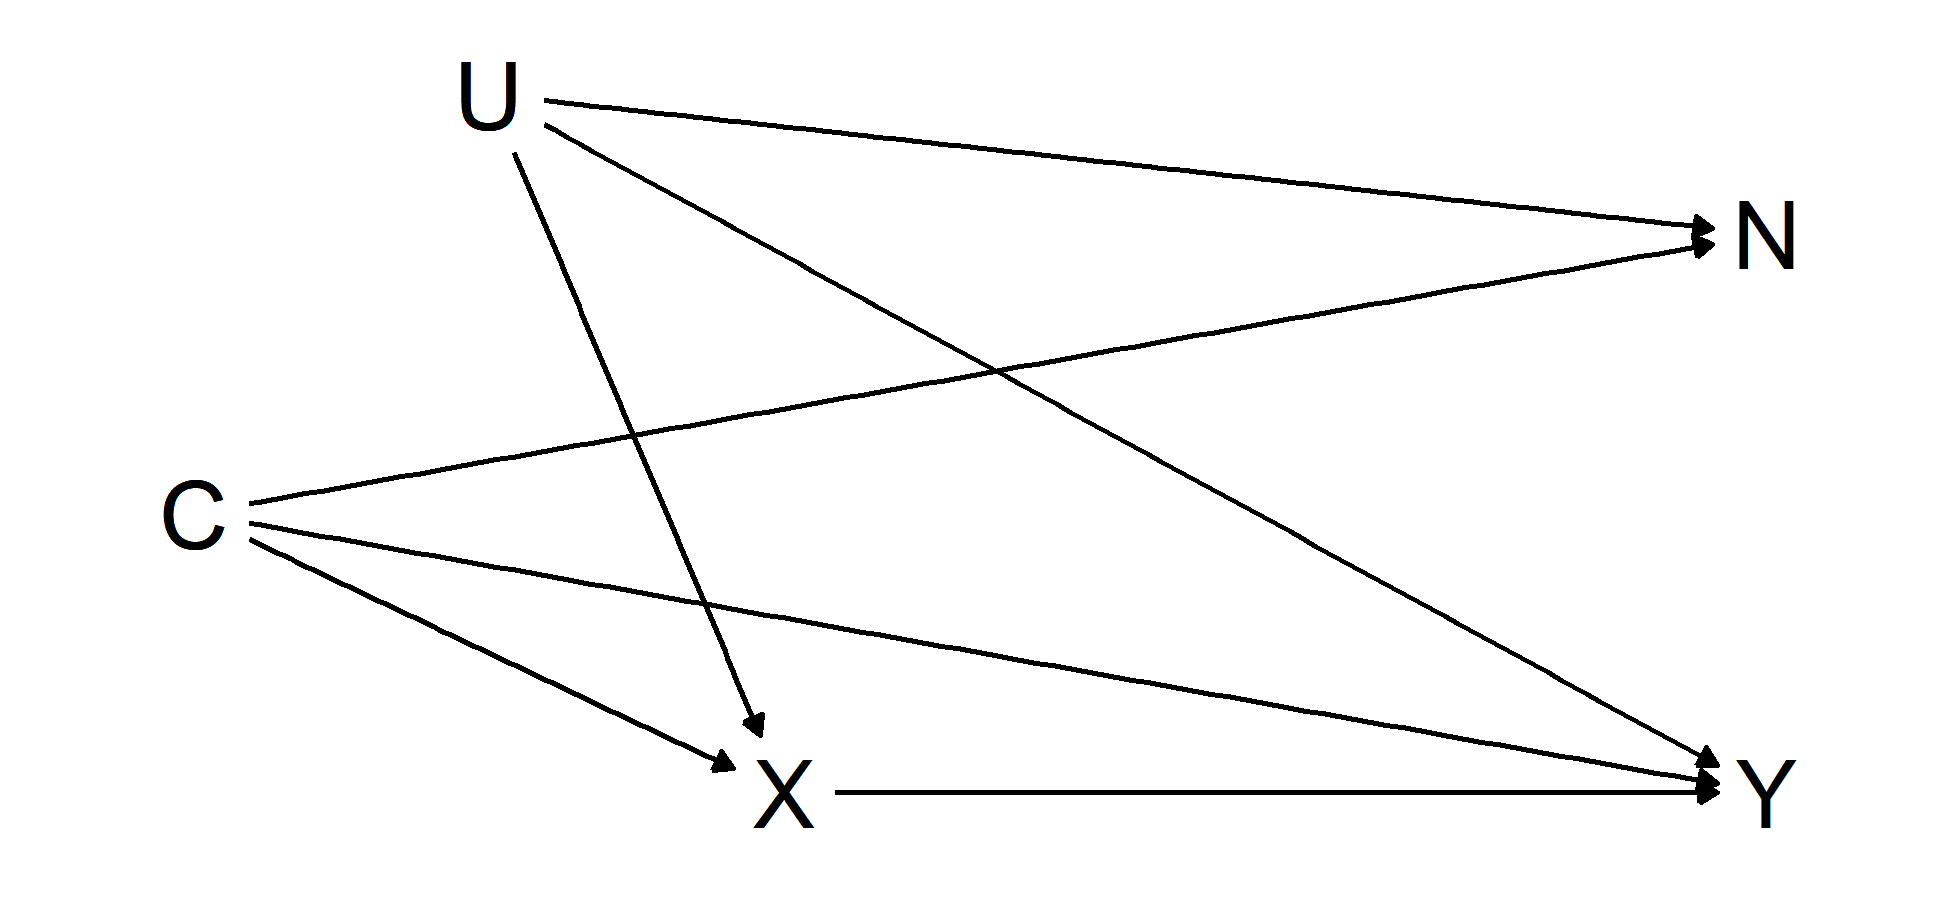
\includegraphics[width=0.8\linewidth]{figures/cprd-analysis/negativeOutcome} 

}

\caption[Causal diagram for ideal negative outcome]{Causal diagram (directed acyclic graph) showing relationship between exposure \(X\), outcome \(Y\), confounders (measured \(C\) and unmeasured \(U\)) and an ideal negative outcome \(N\). Note the absence of any arrow between \(X\) and \(N\). In this scenario, any association observed between \(X\) and \(N\) is due to the presence of uncontrolled confounders \(U\) (assuming \(C\) has been adjusted for).}\label{fig:negativeOutcome}
\end{figure}

~

Despite observational analyses suggesting a link between statins and muscular pain (as opposed to more serious complications such as myopathy),\textsuperscript{\protect\hyperlink{ref-selva-ocallaghan2018}{304}} systematic reviews of the adverse events of statin use\textsuperscript{\protect\hyperlink{ref-collins2016}{37}} and N-of-1 trials explicitly exploring the association of statin use with muscle pain\textsuperscript{\protect\hyperlink{ref-herrett2021}{305}} have found little evidence supporting an effect. This suggests that muscular backpain would be suitable for use as a negative control outcome in this analysis. Under this approach, if statin use is found to be associated with muscular backpain in this analysis, this suggests the presence of residual confounding and reduces my confidence in the results for the dementia outcomes.

Similarly, incident ischemic heart disease and Type 2 diabetes were included as a protective and harmful positive control outcome, respectively. The protective effect of lipid-lowering treatment, via statins, on the risk of ischemic heart disease is well-established,\textsuperscript{\protect\hyperlink{ref-collins2016}{37}} while there is growing evidence for an increased risk of Type 2 diabetes with statin use.\textsuperscript{\protect\hyperlink{ref-collins2016}{37},\protect\hyperlink{ref-macedo2014}{306},\protect\hyperlink{ref-smit2020}{307}} Similar to the negative outcome, if the analysis strategy can reproduce these known associations, this will provide evidence that potential confounders have been sufficiently adjusted for.

~

\hypertarget{impact-of-additional-covariates}{%
\subsubsection{Impact of additional covariates}\label{impact-of-additional-covariates}}

To observe the effect of adjusting for additional covariates, I ran two additional models unadjusted except for: (a) age; and (b) age and gender. The results of these models was then compared the results with the fully adjusted model.

~

\hypertarget{sensitivity-cohorts}{%
\subsubsection{Sensitivity cohorts}\label{sensitivity-cohorts}}

Two sensitivity cohorts were also created. The first stratified by year of entry into the cohort in an attempt to assess for time period effects. The second removed participants who may have been pregnant (coded as under 55) to assess the robustness of the estimates, as statins are contraindicated in pregnancy.\textsuperscript{\protect\hyperlink{ref-karalis2016}{308}}

~

\hypertarget{statin-properties}{%
\subsubsection{Statin properties}\label{statin-properties}}

As detailed in the introduction, the properties of statins may be important in their effect based on the ability of lipophilic statins to cross the blood brain barrier (see Section \ref{intro-statins}).\textsuperscript{\protect\hyperlink{ref-sierra2011}{40}} As such, I expected that any effects of statins on dementia outcomes would be stronger in the lipophilic as compared to the hydrophilic statin subgroup. To investigate this, I further stratified the statin exposure group into lipophilic (Atorvastatin, Lovastatin, Simvastatin, Cerivastatin) and hydrophilic (Pravastatin, Rosuvastatin, Fluvastatin) statins.

~

\hypertarget{impact-of-using-different-code-lists-for-defining-dementia-outcomes}{%
\subsubsection{Impact of using different code lists for defining dementia outcomes}\label{impact-of-using-different-code-lists-for-defining-dementia-outcomes}}

As part of an exploratory analysis of the effect of the choice of code lists on the analysis, I created an alternative Alzheimer's disease and non-Alzheimer's dementia outcome using code lists from a published study by Smeeth \emph{et al}.\textsuperscript{\protect\hyperlink{ref-smeeth2009}{210}} The intended purpose of this analysis was to assess the robustness of my results to the choice of code list.

This previous analysis used a propensity matching approach to estimate the association of statins with a range of outcomes in The Health Improvement Network (THIN) database, a alternative source of English electronic health records which has substantial overlap with the CPRD.\textsuperscript{\protect\hyperlink{ref-carbonari2015}{309}} The code lists used in this analysis were obtained through correspondence with the authors of that study, and are available for inspection (see Section \ref{cprd-data-avail}).

~

\hypertarget{results-1}{%
\section{Results}\label{results-1}}

\hypertarget{patient-characteristics}{%
\subsection{Patient characteristics}\label{patient-characteristics}}

Of the 3,179,733 participants included in the extract, 1,684,564 met the inclusion criteria (Figure \ref{fig:cprdFlowchart}), with a total follow-up of 10,835,685 patient years at risk.

~





\begin{figure}[H]
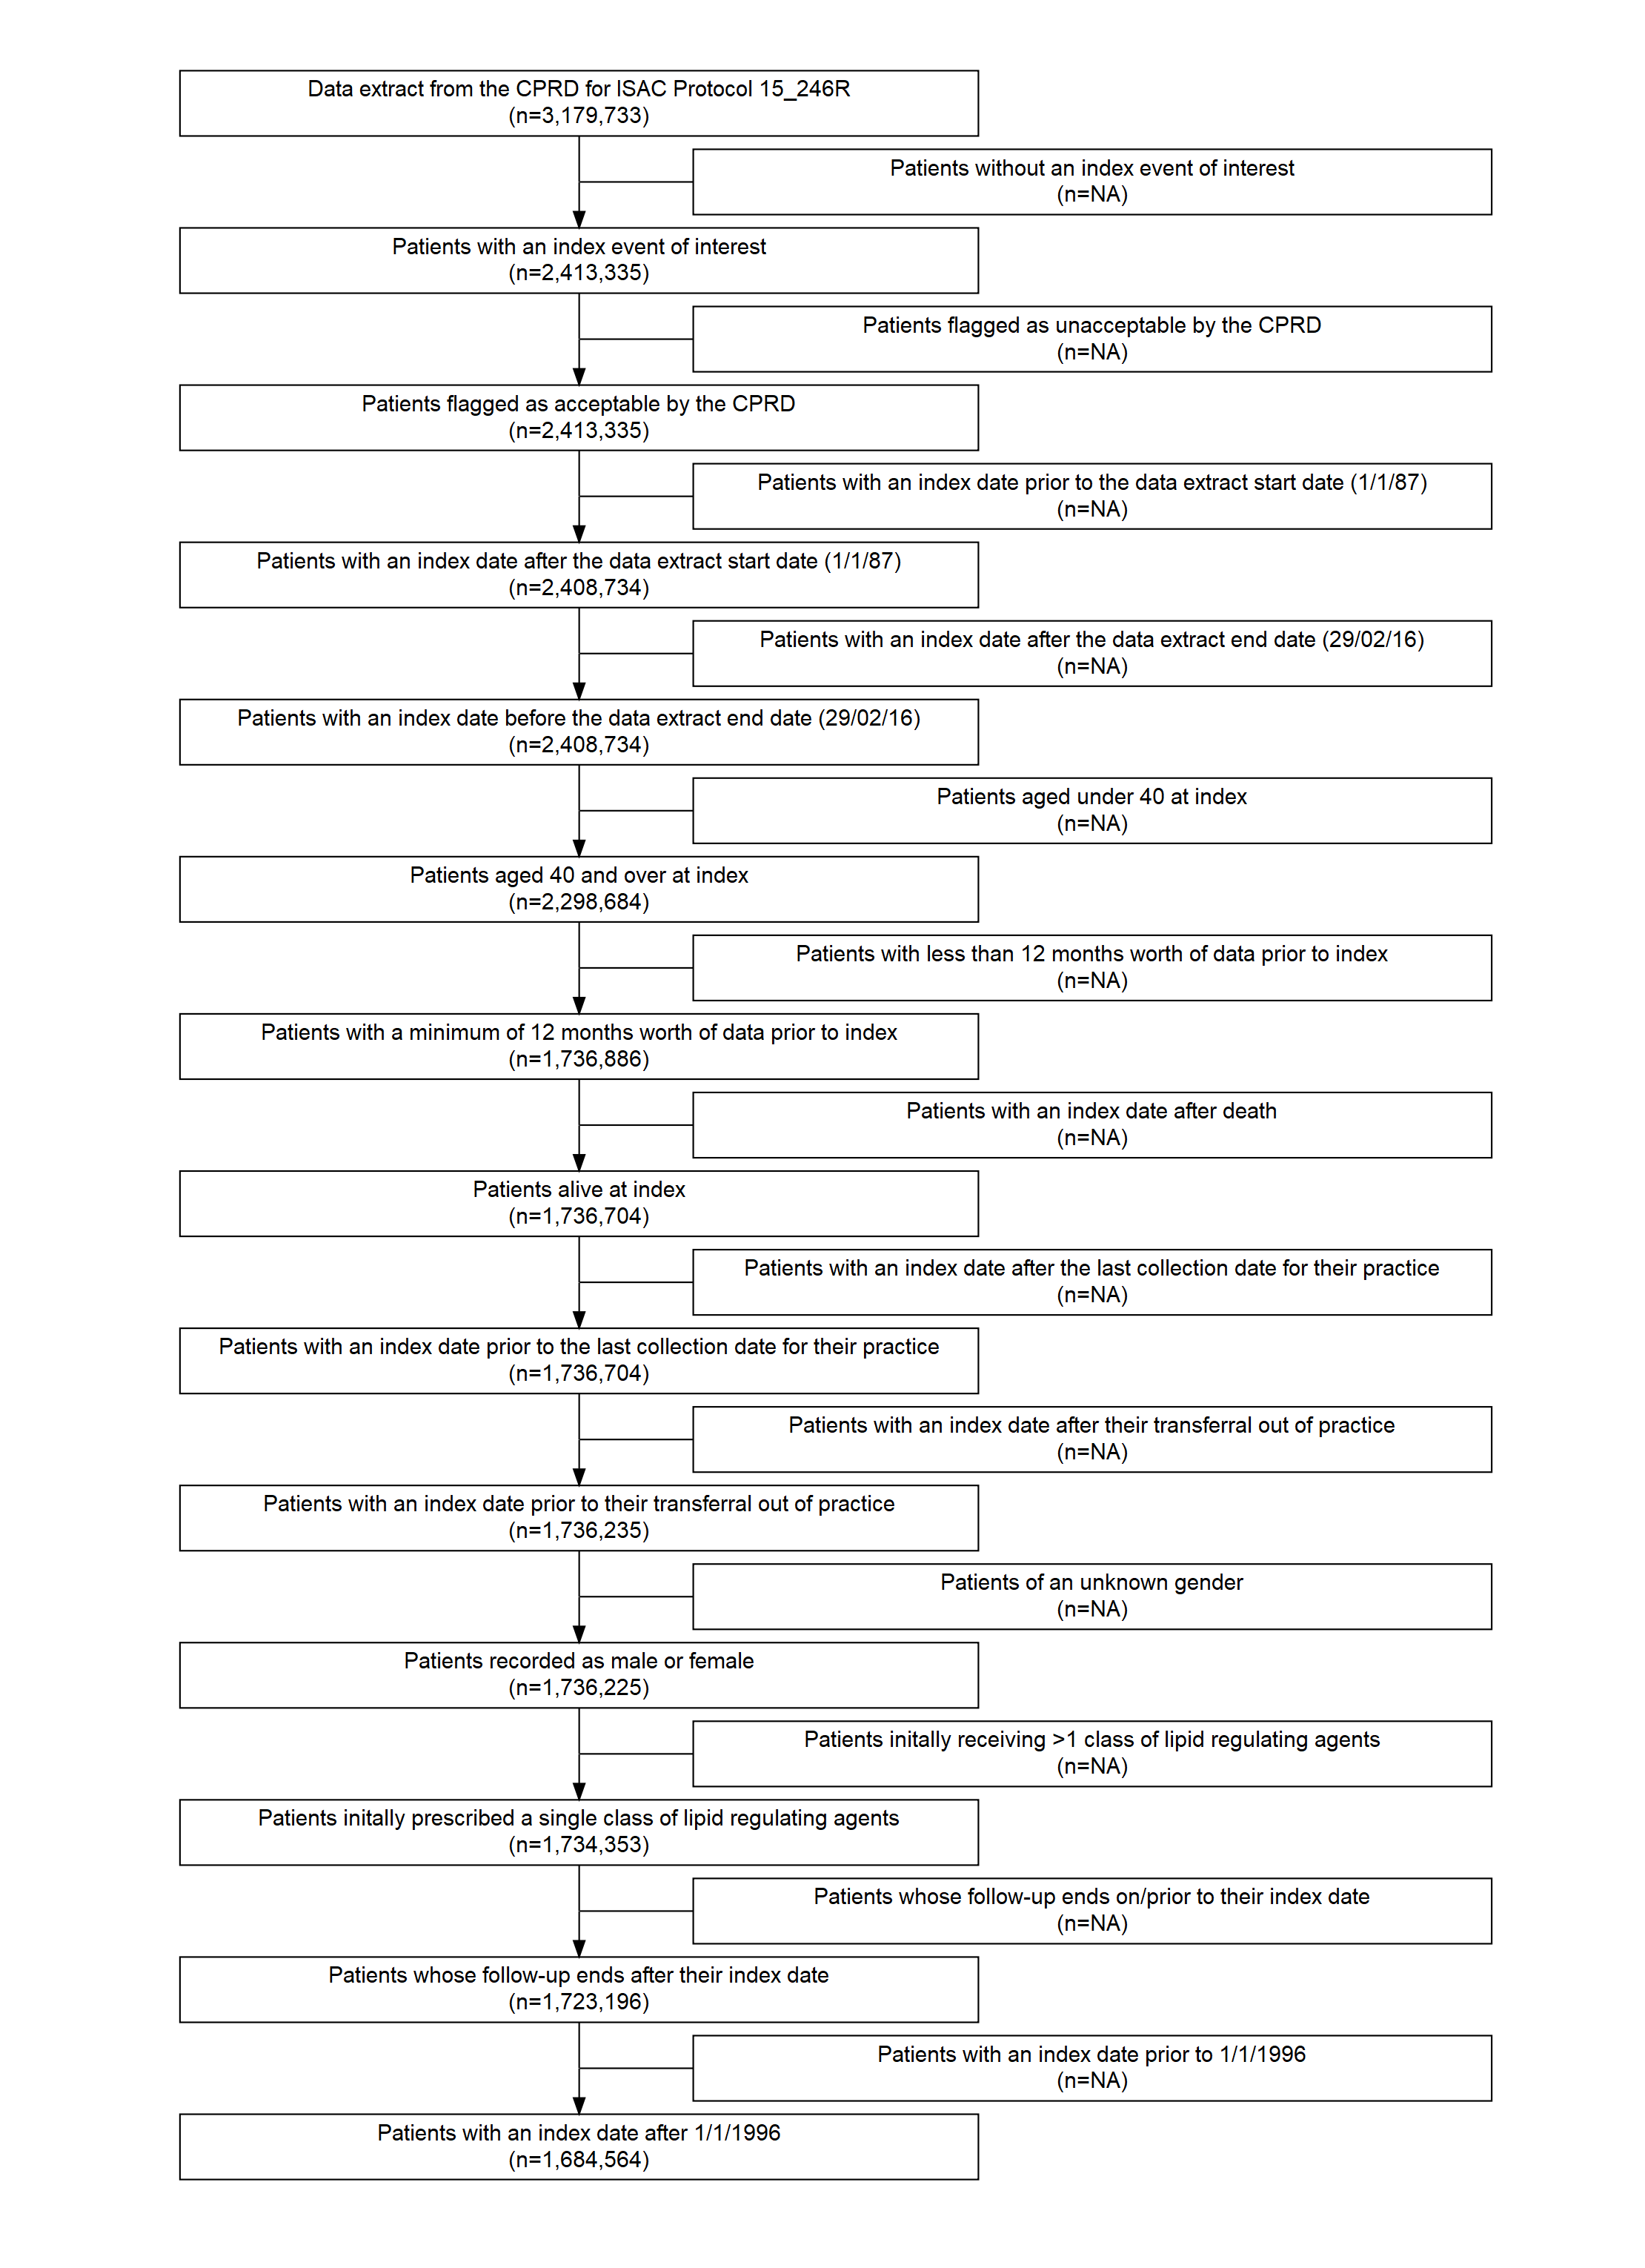
\includegraphics[width=1\linewidth]{figures/cprd-analysis/cohort_attrition} \caption[Attrition of CPRD participants]{Attrition of CPRD participants as the eligibility criteria were applied. The largest cause of attrition was the absence of an index event of interest.}\label{fig:cprdFlowchart}
\end{figure}

~

The median participant age at index was 57 years (inter-quartile range (IQR):48-67years ) and participants were followed up for a median of 5.9 years (IQR:2.7-9.7years ). During follow-up, an all-cause dementia diagnosis was recorded for 41,830 patients (12,647 probable AD, 9,954 possible AD, 8,466 vascular dementia, 10,763 other dementias).

The number of events, time-at-risk and crude rates for each drug class, tabulated by dementia outcome, are shown in Table \ref{tab:followUp-table}. A substantial majority (98.1\%) of participants prescribed a lipid-regulating agent were prescribed a statin. I excluded the ``Ezetimibe and statins'' (n=127) and ``Nicotinic acid groups'' (n= 165) classes from subsequent class-based subgroup analyses based on the extremely small number of participants in these groups. Note that the ``Ezetimibe and statins'' treatment group represent those prescribed a single treatment containing both ezetimibe and statins, rather than those where the two treatments were prescribed concurrently.

\blandscape





\begin{table}

\caption[Crude rates, stratified by outcome and drug class of interest.]{\label{tab:followUp-table}Summary of number of events, years at risk and crude rates per 100,000 participant-years-at-risk stratified by dementia outcome and drug class of interest.}
\centering
\fontsize{8}{10}\selectfont
\begin{threeparttable}
\begin{tabular}[t]{>{}l|>{\centering\arraybackslash}p{3em}>{\centering\arraybackslash}p{3em}>{}c|>{\centering\arraybackslash}p{3em}>{\centering\arraybackslash}p{3em}>{}c|>{\centering\arraybackslash}p{3em}>{\centering\arraybackslash}p{3em}>{}c|>{\centering\arraybackslash}p{3em}>{\centering\arraybackslash}p{3em}>{}c|>{\centering\arraybackslash}p{3em}>{\centering\arraybackslash}p{3em}>{\centering\arraybackslash}p{3em}}
\toprule
\multicolumn{1}{c}{\textbf{ }} & \multicolumn{3}{c}{\textbf{Any dementia}} & \multicolumn{3}{c}{\textbf{Possible AD}} & \multicolumn{3}{c}{\textbf{Probable AD}} & \multicolumn{3}{c}{\textbf{Vascular dementia}} & \multicolumn{3}{c}{\textbf{Other dementia}} \\
\cmidrule(l{3pt}r{3pt}){2-4} \cmidrule(l{3pt}r{3pt}){5-7} \cmidrule(l{3pt}r{3pt}){8-10} \cmidrule(l{3pt}r{3pt}){11-13} \cmidrule(l{3pt}r{3pt}){14-16}
\textbf{Exposure Group} & \textbf{Events} & \textbf{PYAR} & \textbf{Rate \textsuperscript{*}} & \textbf{Events} & \textbf{PYAR} & \textbf{Rate \textsuperscript{*}} & \textbf{Events} & \textbf{PYAR} & \textbf{Rate \textsuperscript{*}} & \textbf{Events} & \textbf{PYAR} & \textbf{Rate \textsuperscript{*}} & \textbf{Events} & \textbf{PYAR} & \textbf{Rate \textsuperscript{*}}\\
\midrule
\textbf{No LRA (unexposed)} & 18,608 & 5,872,717 & 317 & 6,368 & 5,818,047 & 109 & 2,637 & 5,800,964 & 45 & 4,813 & 5,811,594 & 83 & 4,790 & 5,808,285 & 82\\
\textbf{By drug class} &  &  &  &  &  &  &  &  &  &  &  &  &  &  & \\
\hspace{1em}Statins & 22,920 & 4,871,568 & 470 & 6,190 & 4,758,526 & 130 & 5,773 & 4,753,437 & 121 & 5,871 & 4,755,258 & 123 & 5,086 & 4,747,237 & 107\\
\hspace{1em}Omega-3 FAGs & 19 & 8,034 & 236 & 4 & 7,927 & 50 & 7 & 7,950 & 88 & 4 & 7,938 & 50 & 4 & 7,925 & 50\\
\hspace{1em}Fibrates & 141 & 38,003 & 371 & 49 & 37,102 & 132 & 21 & 36,835 & 57 & 36 & 37,001 & 97 & 35 & 36,983 & 95\\
\hspace{1em}Ezetimibe & 32 & 6,604 & 485 & 8 & 6,429 & 124 & 7 & 6,425 & 109 & 12 & 6,444 & 186 & 5 & 6,393 & 78\\
\hspace{1em}BAS & 106 & 36,370 & 291 & 28 & 35,808 & 78 & 19 & 35,726 & 53 & 26 & 35,768 & 73 & 33 & 35,808 & 92\\
\hspace{1em}Ezetimibe + Statins \textsuperscript{\dag} & 0 & 986 & - & 0 & 986 & - & 0 & 986 & - & 0 & 986 & - & 0 & 986 & -\\
\hspace{1em}NAG & 4 & 1,403 & - & 0 & 1,379 & - & 2 & 1,391 & - & 1 & 1,389 & - & 1 & 1,382 & -\\
\midrule
\textbf{Total} & 41,830 & 10,835,686 & 386 & 12,647 & 10,666,205 & 119 & 8,466 & 10,643,714 & 80 & 10,763 & 10,656,378 & 101 & 9,954 & 10,644,999 & 94\\
\bottomrule
\end{tabular}
\begin{tablenotes}
\item \textsuperscript{*} Crude rate per 100,000 participant-years-at-risk\newline \textsuperscript{\dag} One treatment containing both drugs, rather than the two classes being prescribed concurrently\newline \textbf{Abbreviations:} AD - Alzheimer's disease;  BAS - Bile acid sequestrants; LRA - Lipid regulating agent;  NAG - Nicotinic acid groups;  Omega-3 FGs - Omega-3 Fatty acid groups; PYAR - Participant-years-at-risk.
\end{tablenotes}
\end{threeparttable}
\end{table}





\begin{table}[H]

\caption[Patient characteristics by drug class]{\label{tab:cprdCharacteristics-table}Patient characteristics by drug class. Summary statistics are presented as ``\% (N)'' unless otherwise specified in the variable name.}
\centering
\fontsize{7}{9}\selectfont
\begin{threeparttable}
\begin{tabular}[t]{>{\raggedright\arraybackslash}p{15em}>{\centering\arraybackslash}p{7.7em}>{\centering\arraybackslash}p{7.7em}>{\centering\arraybackslash}p{7.7em}>{\centering\arraybackslash}p{7.7em}>{\centering\arraybackslash}p{7.7em}>{\centering\arraybackslash}p{7.7em}>{\centering\arraybackslash}p{7.7em}}
\toprule
\textbf{ } & \textbf{Whole Sample} & \textbf{None} & \textbf{Statins} & \textbf{Bile acid sequestrants} & \textbf{Ezetimibe} & \textbf{Fibrates} & \textbf{Omega-3 Fatty Acid Groups}\\
\midrule
\textbf{Sample size (N)} & 1,684,564 & 1,087,704 & 585,528 & 5,396 & 763 & 3,889 & 992\\
\midrule
\textbf{Year of cohort entry \newline (median)} & 2006 & 2007 & 2004 & 2005 & 2004 & 2001 & 2005\\
\midrule
\textbf{Female} & 53.0\% (893174) & 56.2\% (610950) & 47.1\% (276043) & 66.4\% (3585) & 54.5\% (416) & 38.6\% (1500) & 52.6\% (522)\\
\midrule
\textbf{Age at cohort entry \newline (median)} & 57 & 54 & 62 & 57 & 60 & 58 & 56\\
\midrule
\textbf{CAD} & 0.4\% (7133) & 0.1\% (589) & 1.1\% (6465) & 0.1\% (6) & 0.9\% (7) & 1.4\% (53) & 1.3\% (13)\\
\midrule
\addlinespace
\textbf{CBS} & 0.3\% (5699) & 0.1\% (682) & 0.8\% (4926) & 0.1\% (4) & 0.4\% (3) & 2.0\% (78) & 0.6\% (6)\\
\midrule
\textbf{CVD} & 2.1\% (34899) & 1.1\% (11619) & 3.9\% (22977) & 1.6\% (86) & 2.6\% (20) & 4.4\% (170) & 1.7\% (17)\\
\midrule
\textbf{Charlson (ever > 0)} & 30.6\% (516135) & 25.1\% (272642) & 40.7\% (238403) & 42.5\% (2292) & 41.7\% (318) & 50.8\% (1976) & 40.4\% (401)\\
\midrule
\textbf{IMD-2010 (median)} & 9 & 8 & 9 & 8 & 9 & 10 & 10\\
\midrule
\textbf{Consultation rate (mean/SD)} & 5.4 (5.4) & 5.0 (5.0) & 6.2 (6.1) & 8.6 (7.4) & 7.4 (6.6) & 7.1 (6.2) & 8.0 (8.0)\\
\midrule
\addlinespace
\textbf{Alcohol (ever)} & 85.9\% (1447151) & 86.6\% (941648) & 84.7\% (496110) & 82.8\% (4468) & 84.0\% (641) & 82.9\% (3223) & 82.0\% (813)\\
\midrule
\textbf{Smoking (ever)} & 51.1\% (861355) & 47.1\% (511826) & 58.6\% (343074) & 55.2\% (2978) & 57.5\% (439) & 60.2\% (2341) & 53.7\% (533)\\
\midrule
\textbf{BMI (mean/SD)} & 27.0 (5.3) & 26.7 (5.2) & 27.7 (5.3) & 26.8 (5.8) & 28.1 (5.7) & 29.0 (5.2) & 26.9 (5.5)\\
\midrule
\textbf{PAD} & 0.7\% (12613) & 0.4\% (4039) & 1.4\% (8424) & 0.9\% (47) & 0.9\% (7) & 1.9\% (75) & 1.0\% (10)\\
\midrule
\textbf{Hypertension} & 16.0\% (269804) & 11.5\% (124604) & 24.4\% (143101) & 12.8\% (692) & 23.9\% (182) & 25.8\% (1002) & 15.7\% (156)\\
\midrule
\addlinespace
\textbf{Total cholesterol (mean/SD)} & 5.7 (10.1) & 5.5 (6.4) & 6.2 (15.3) & 5.3 (1.3) & 7.1 (26.5) & 6.4 (5.6) & 5.6 (1.6)\\
\midrule
\textbf{LDL cholesterol (mean/SD)} & 3.6 (4.9) & 3.4 (5.3) & 4.0 (3.7) & 3.1 (1.0) & 3.9 (1.1) & 3.3 (1.8) & 3.2 (1.0)\\
\midrule
\textbf{CKD} & 0.1\% (1295) & 0.1\% (740) & 0.1\% (545) & 0.1\% (6) & 0.1\% (1) & 0.0\% (0) & 0.3\% (3)\\
\midrule
\textbf{Type 1 Diabetes} & 0.2\% (4037) & 0.1\% (785) & 0.5\% (3196) & 0.3\% (14) & 1.0\% (8) & 0.8\% (31) & 0.1\% (1)\\
\midrule
\textbf{Type 2 Diabetes} & 2.9\% (48557) & 1.1\% (11797) & 6.1\% (35941) & 2.3\% (123) & 5.4\% (41) & 15.8\% (614) & 2.8\% (28)\\
\bottomrule
\end{tabular}
\begin{tablenotes}
\item \textit{Note:} The 'Nicotinic acid groups' (n=165) and 'Ezetimibe and Statins' (n=127) subgroups are not shown, but are included in the whole sample column\newline \textbf{Abbreviations:} BMI - Body mass index; CAD - Coronary arterial disease; CBS - Coronary bypass surgery; CKD - Chronic kidney disease; CVD - Cardiovascular disease; IMD - Index of multiple deprivation; LRA - Lipid regulating agent; PAD - Peripheral arterial disease; SD - Standard deviation.
\end{tablenotes}
\end{threeparttable}
\end{table}

\elandscape

The distribution of baseline characteristics across the remaining seven drug classes can be seen in Table \ref{tab:cprdCharacteristics-table}. Note due to the experimental design, the median year of entry is expected to be later for those not prescribed an LRA, as this exposure group is more likely to include those who entered into the cohort towards the end of study window (as these people had less follow-up time in which to be prescribed an LRA).

The stopping, addition and switching of drug classes was common across all drug classes (Table \ref{tab:cprdSSA-table}).

~\\




\begin{table}[H]

\caption[Participants who stopped, switched or added treatements by initial treatment type]{\label{tab:cprdSSA-table}Participants who stopped, switched or added treatments by initial treatment type.}
\centering
\fontsize{7}{9}\selectfont
\begin{threeparttable}
\begin{tabular}[t]{>{\raggedright\arraybackslash}p{5em}>{\centering\arraybackslash}p{4.225em}>{\centering\arraybackslash}p{4.225em}>{\centering\arraybackslash}p{4.225em}>{\centering\arraybackslash}p{4.225em}>{\centering\arraybackslash}p{4.225em}>{\centering\arraybackslash}p{4.225em}>{\centering\arraybackslash}p{4.225em}>{\centering\arraybackslash}p{4.225em}}
\toprule
\textbf{ } & \textbf{Whole Sample} & \textbf{Statins} & \textbf{Bile acid sequestrants} & \textbf{Ezetimibe} & \textbf{Ezetimibe \& Statins} & \textbf{Fibrates} & \textbf{Nicotinic acid groups} & \textbf{Omega-3 Fatty Acid Groups}\\
\midrule
\textbf{Stopped} & 6.9\% (115899) & 19.1\% (111798) & 56.1\% (3028) & 19.7\% (150) & 12.6\% (16) & 12.3\% (478) & 44.8\% (74) & 35.8\% (355)\\
\midrule
\textbf{Added} & 1.6\% (27441) & 4.4\% (25990) & 3.6\% (192) & 19.0\% (145) & 3.9\% (5) & 21.6\% (841) & 3.6\% (6) & 26.4\% (262)\\
\midrule
\textbf{Switched} & 0.9\% (14935) & 2.0\% (11996) & 11.3\% (612) & 34.6\% (264) & 64.6\% (82) & 44.0\% (1713) & 45.5\% (75) & 19.5\% (193)\\
\bottomrule
\end{tabular}
\begin{tablenotes}
\item \textbf{Defintions:} Stopped - last prescription of the primary drug class followed by at least six months of observation with no further prescriptions; Added - second drug class prescribed before the last prescription of the initial class; Switched - second drug class being prescribed after the last prescription of the initial class.
\end{tablenotes}
\end{threeparttable}
\end{table}

~

\hypertarget{missing-data-1}{%
\subsection{Missing data}\label{missing-data-1}}

Full covariate information was available for 450,234 participants (26.7\%). Six key variables had some missing data: IMD 2010 score was missing for 625,788 participants (37.1\%), because it is only recorded for English practices; alcohol status was missing for 269,526 participants (16\%); smoking status was missing for 84,424 participants (5\%); BMI, or a calculated BMI from height and weight measurements, was missing for 266,672 participants (15.8\%); baseline total cholesterol was missing for 119,675 participants (7.1\%); and baseline LDL cholesterol was missing for 787,289 participants (46.7\%).

~

\hypertarget{primary-analysis}{%
\subsection{Primary analysis}\label{primary-analysis}}

The results of the primary analysis using the fully adjusted Cox proportional hazards model with participant age as the time scale are presented for each drug/outcome combination in Figure \ref{fig:cprdPrimary}.

For each outcome, the overall ``Any drug'' estimate was driven by the statin subgroup, based on its large size relative to the other drug classes.

~





\begin{figure}[H]
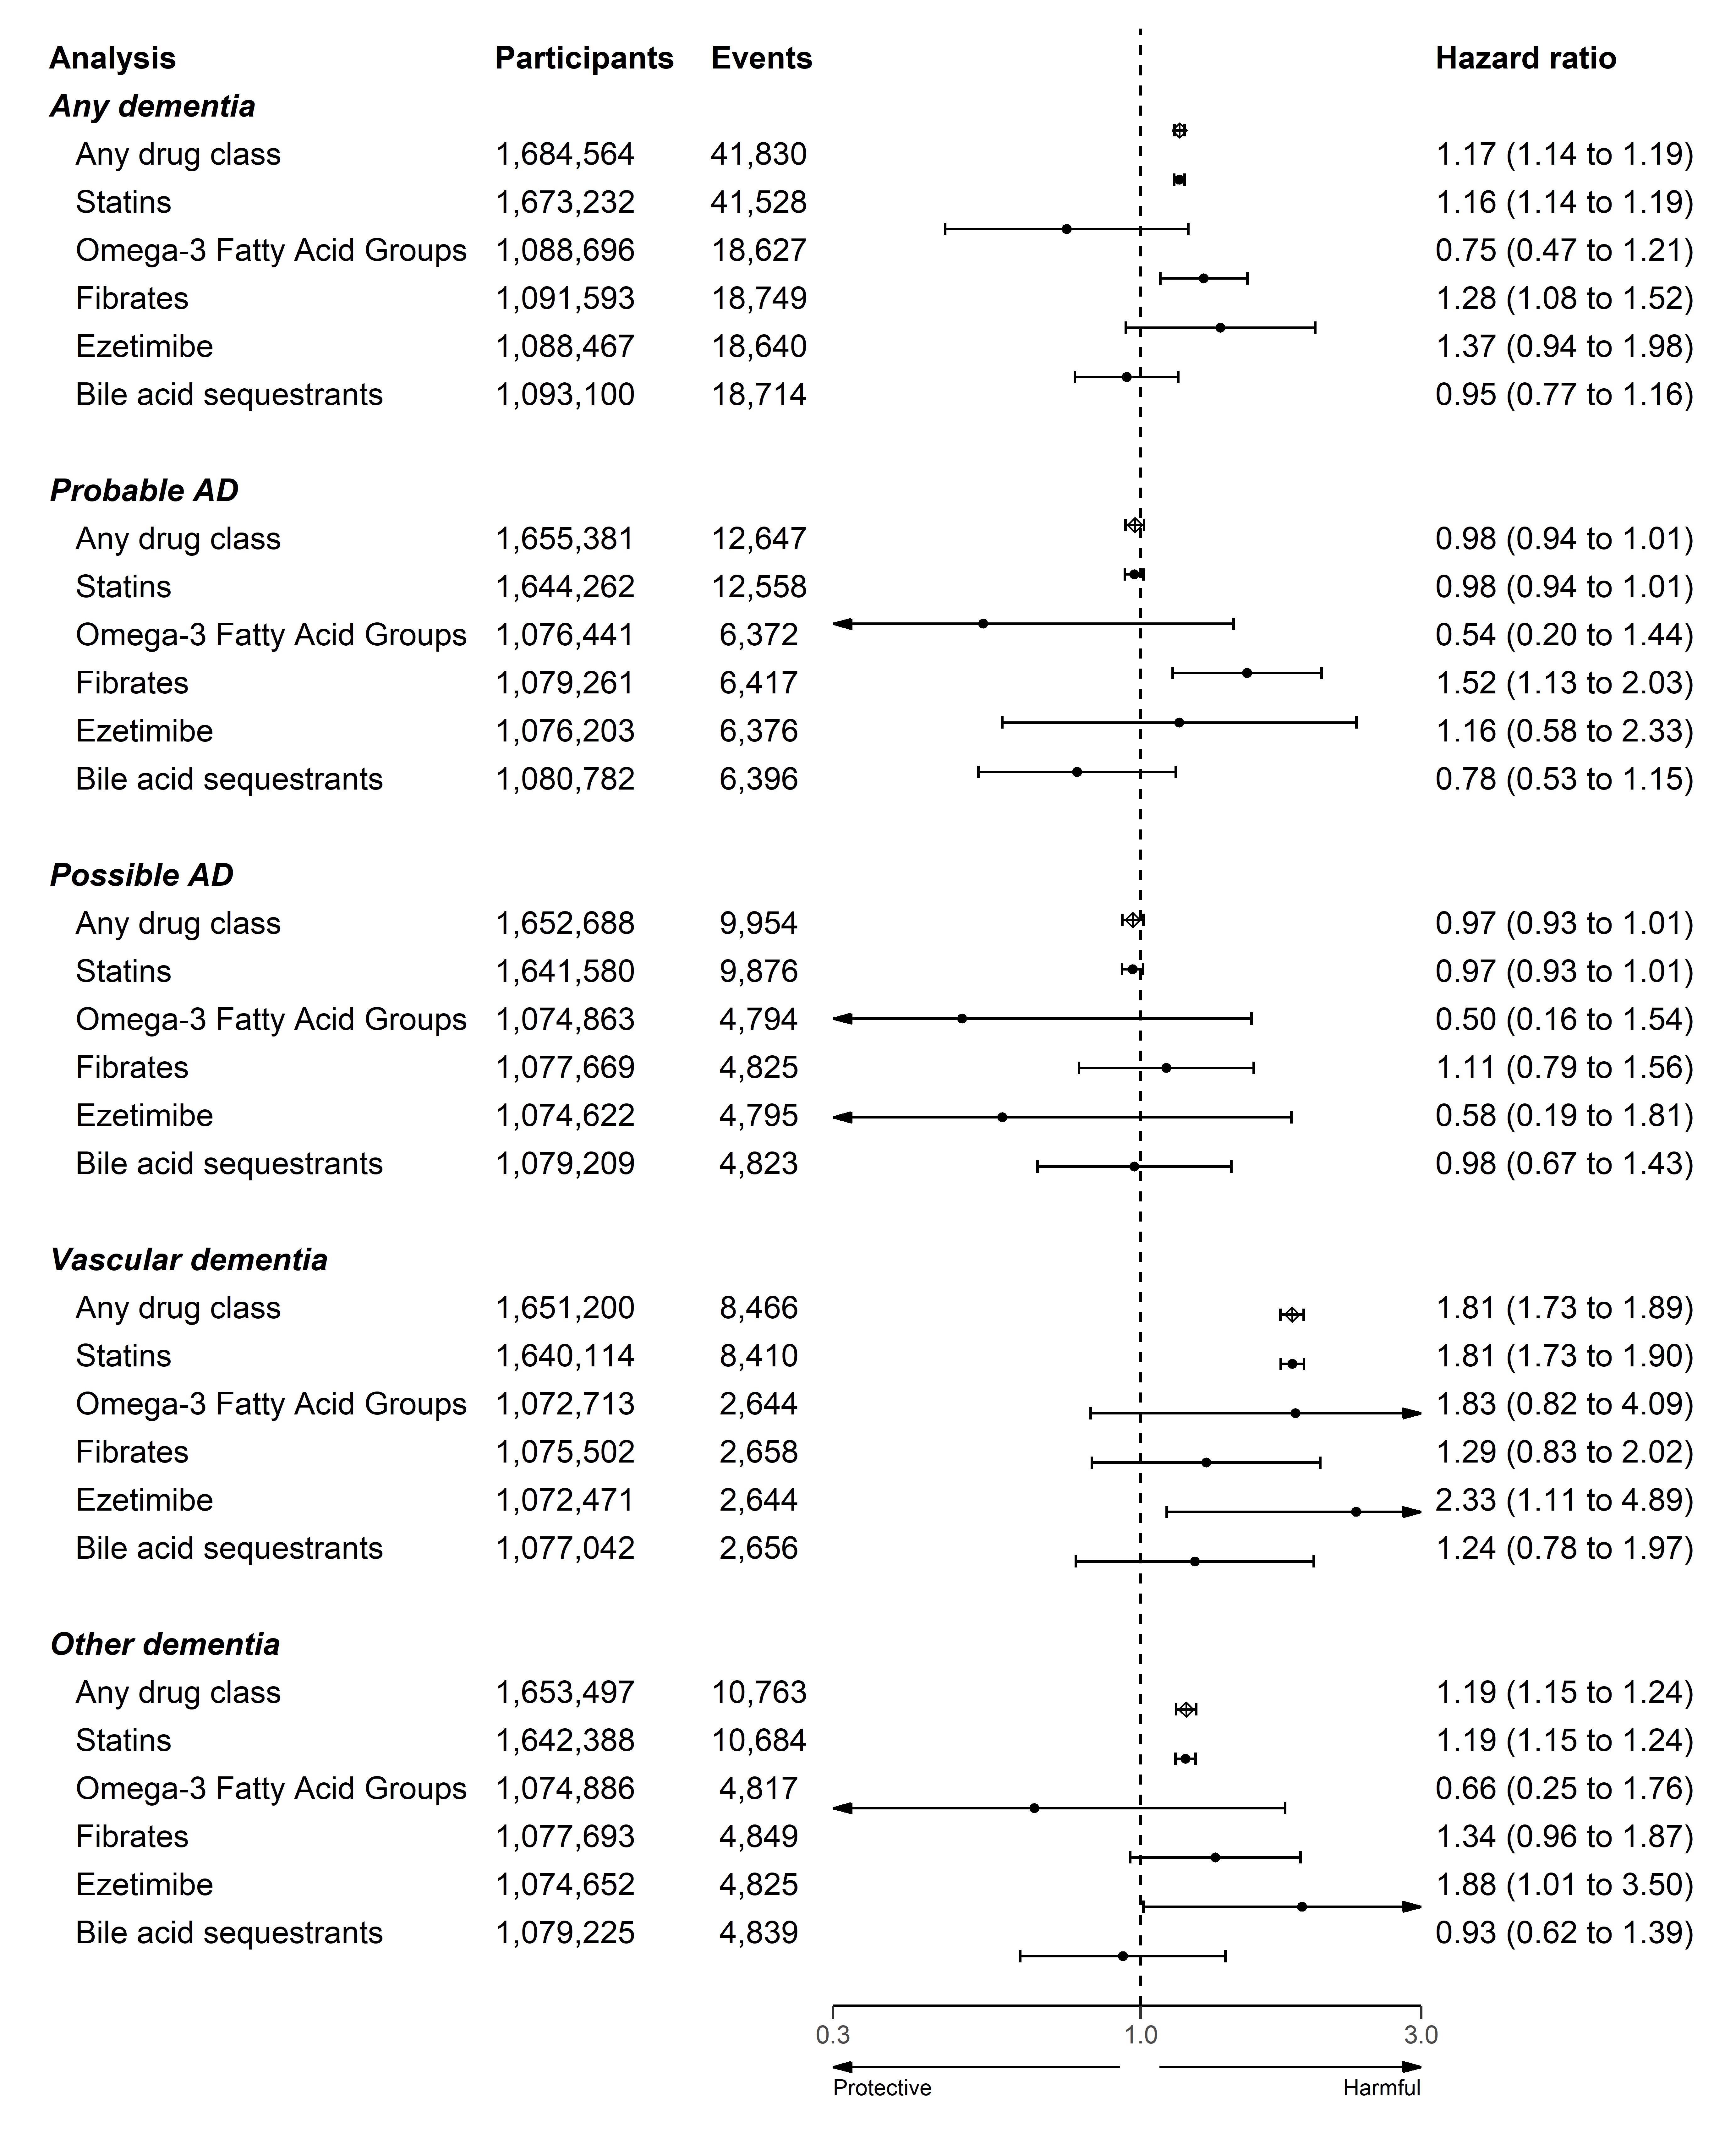
\includegraphics[width=1\linewidth]{figures/cprd-analysis/forester_p1} \caption[Results from primary analyses of CPRD data]{Results from primary analyses of CPRD data using the fully adjusted model and participant age as the time scale.}\label{fig:cprdPrimary}
\end{figure}

~

\textbf{Alzheimer's disease}

My results show litte evidence was found for an effect of lipid-regulating agents on probable (HR:0.98, 95\%CI:0.94-1.01) and possible (HR:0.97, 95\%CI:0.93-1.01) Alzheimer's disease when compared to no treatment, with the sole exception of fibrates on probable Alzheimer's disease (HR:1.52, 95\%CI:1.13-2.03).

~

\textbf{Non-Alzheimer's disease dementias}

In contrast to the findings for Alzheimer's disease outcomes, lipid-regulating agents were associated with an increased risk of a subsequent diagnosis of vascular dementia (HR:1.81, 95\%CI:1.73-1.89) or other dementias (HR:1.19, 95\%CI:1.15-1.24). Again this effect was driven mainly by the statin subgroup, but there was some evidence that ezetimibe was associated with an increased risk of vascular (HR:2.33, 95\%CI:1.11-4.89) and other (HR:1.88, 95\%CI:1.01-3.5) dementia.

~

\textbf{All-cause dementia}

For the composite all-cause dementia outcome, we found treatment with a lipid-regulating agent was associated with a slightly increased risk (HR:1.17, 95\%CI:1.14-1.19), which lies between the associations for the Alzheimer and non-Alzheimer dementia outcomes as would be expected. There was also some evidence that fibrates were associated with increased risk of all-cause dementia (HR:1.28, 95\%CI:1.08-1.52).

~

\hypertarget{sensitivity-analyses-1}{%
\subsection{Sensitivity analyses}\label{sensitivity-analyses-1}}

The results of the series of sensitivity analyses performed are described in the following sections.

\hypertarget{complete-case-versus-imputed-data}{%
\subsubsection{Complete case versus imputed data}\label{complete-case-versus-imputed-data}}

In almost all cases, the use of imputed data resulted in a marginal attenuation of the effects observed when using a complete cases analysis. It should be noted that due to the large amount of missing data (e.g.~787,289 participants (46.7\%) were missing a baseline LDL cholesterol measure), the number of participants included in the complete case analysis was substantially smaller than that included when using imputed data. In this case, though the overall position of the effect estimates does not change substantially when using the imputed dataset, there is a noticeable gain in power.\textsuperscript{\protect\hyperlink{ref-sterne2009}{295}}

~





\begin{figure}[H]
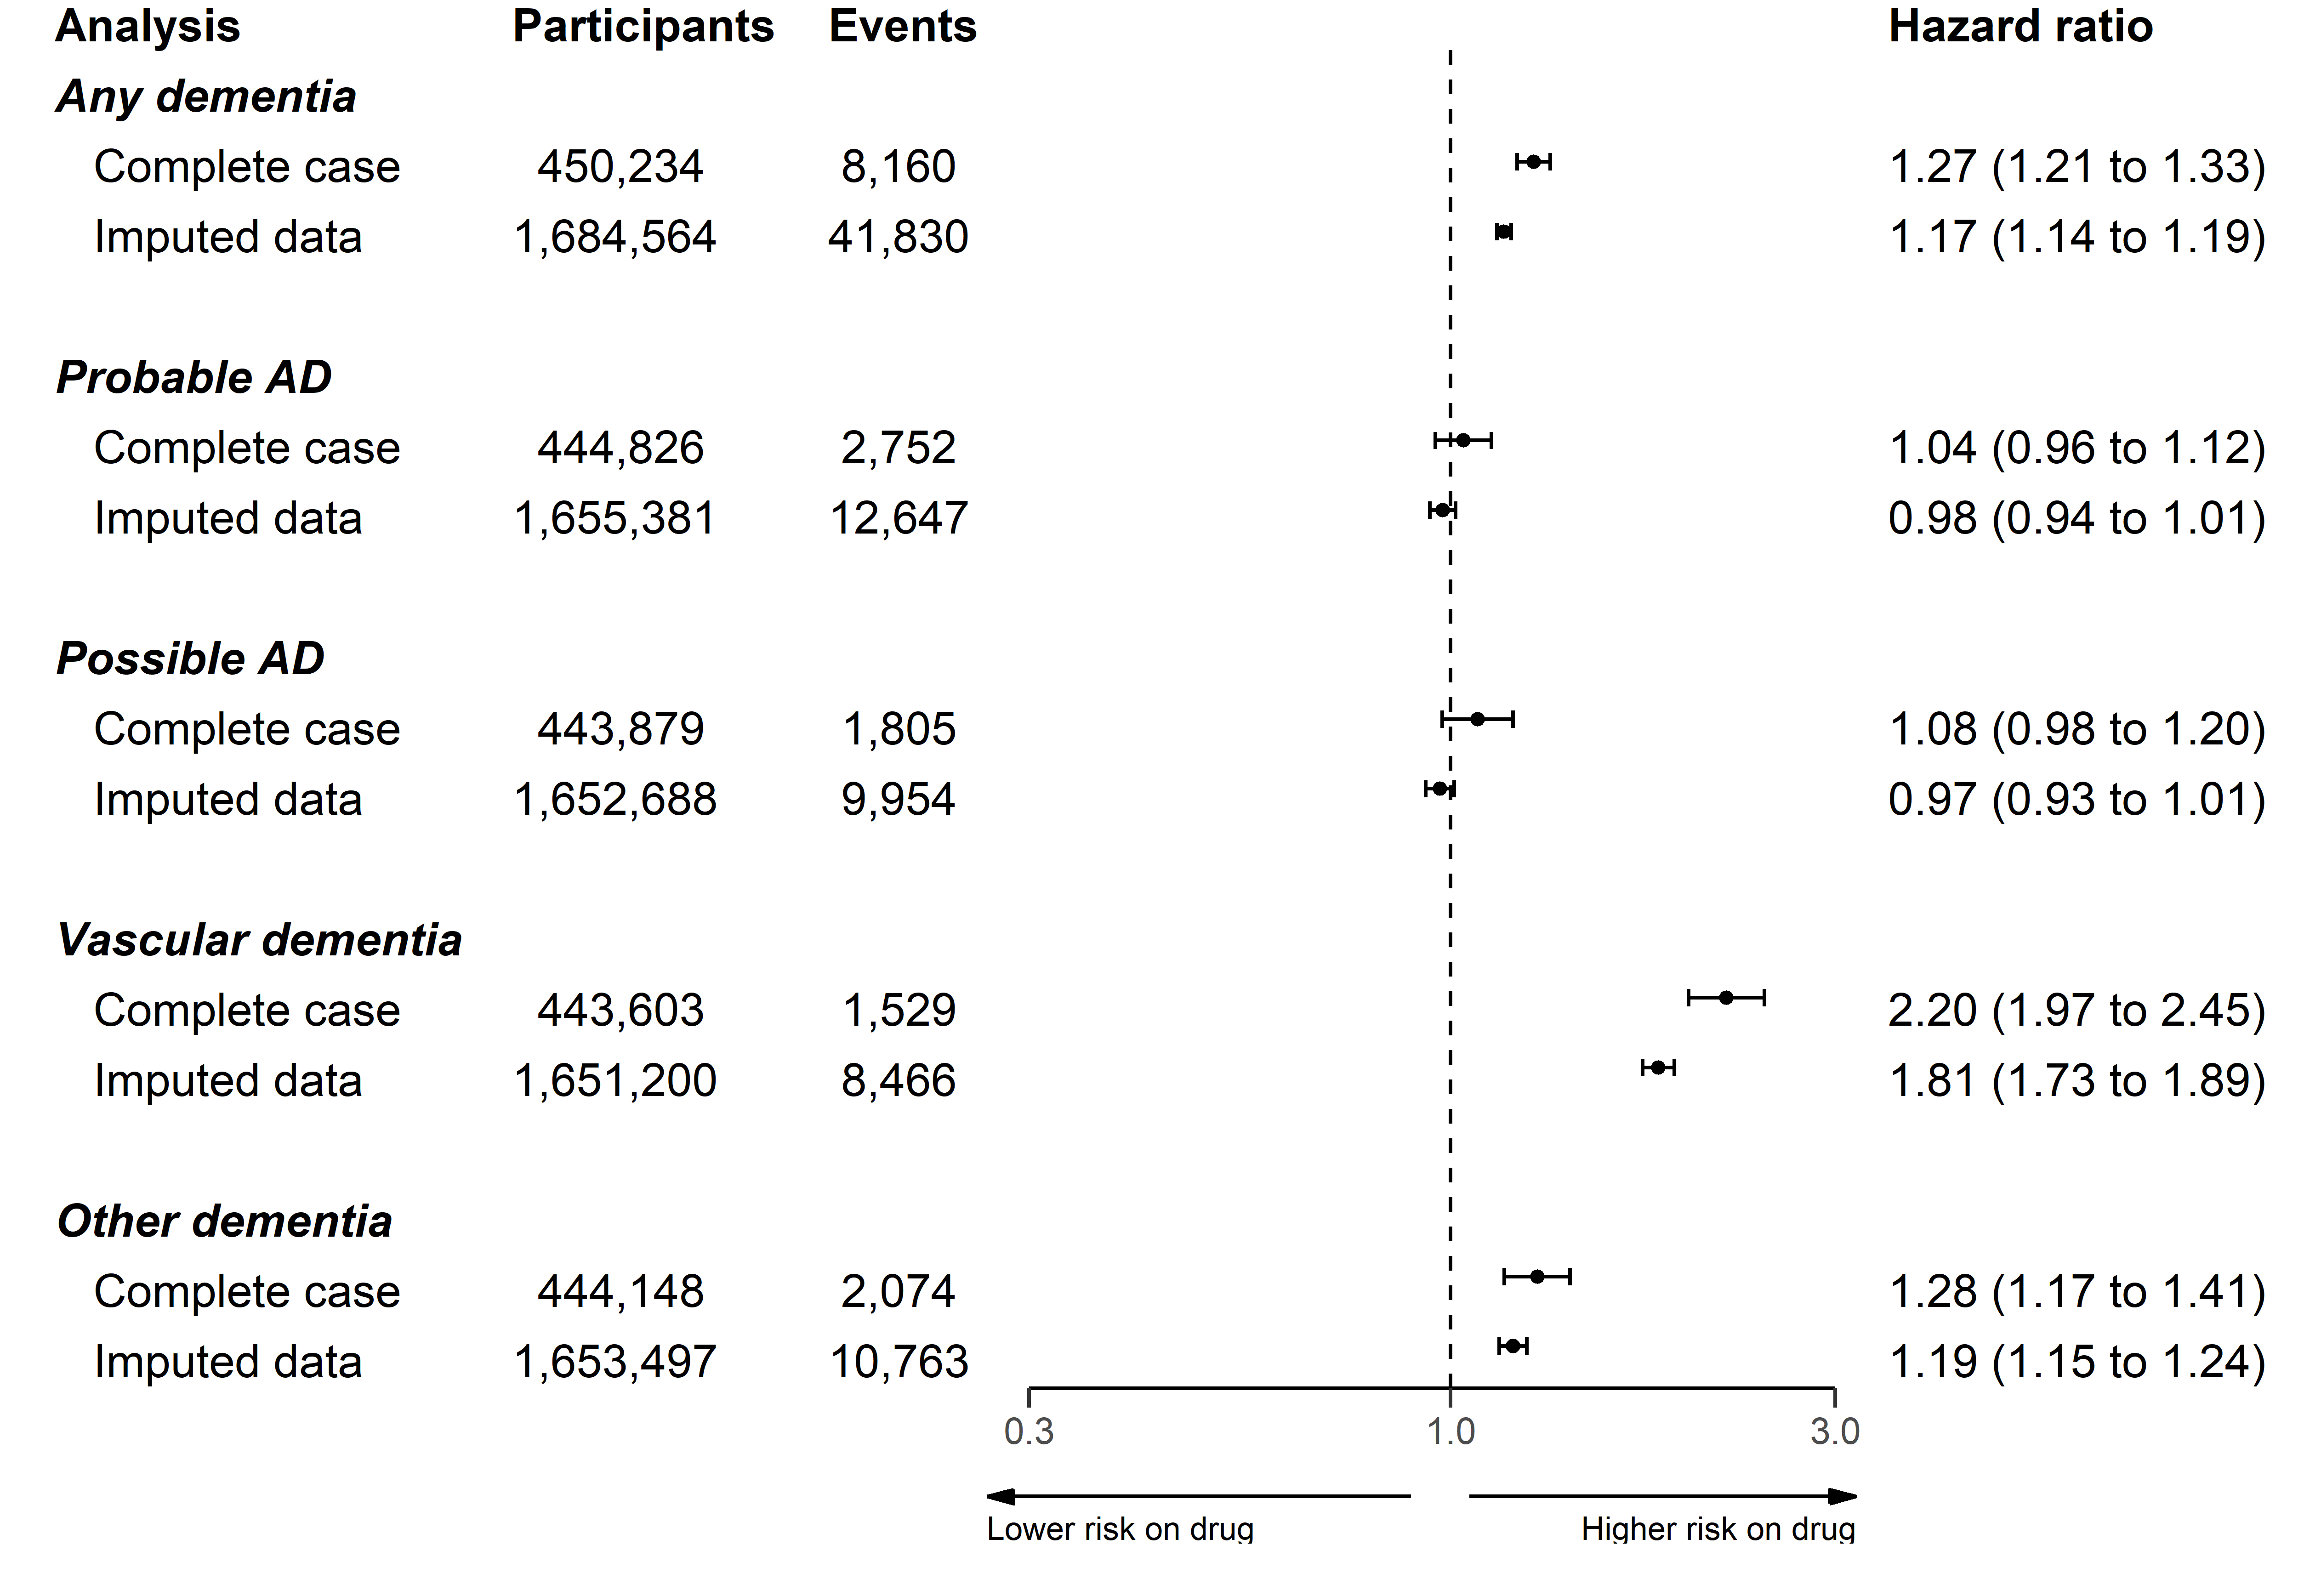
\includegraphics[width=1\linewidth]{figures/cprd-analysis/forester_complete_case} \caption[Complete case vs.~imputed data analysis]{Comparison of analyses using the complete case versus imputed cohorts.}\label{fig:completeCaseFig}
\end{figure}

~

\hypertarget{control-outcomes-1}{%
\subsubsection{Control outcomes}\label{control-outcomes-1}}

Following the primary analysis, the fully adjusted model was used to estimate the effect of treatment with a statin on the two control outcomes of back pain (negative) and ischemic heart disease (positive). The results of this analysis are presented in Figure \ref{fig:controlOutcomeFig}.

For the negative control, there was some evidence that treatment with a statin was associated with an increased risk of back pain (HR: 1.04, 95\%CI: 1.03-1.05), suggesting there may be some residual confounding. However, statin prescription was also associated with a substantially increased risk of ischemic heart disease (HR: 1.62, 95\%CI: 1.59-1.64) and Type 2 diabetes (HR: 1.50, 95\%CI: 1.48-1.51).

~





\begin{figure}[H]
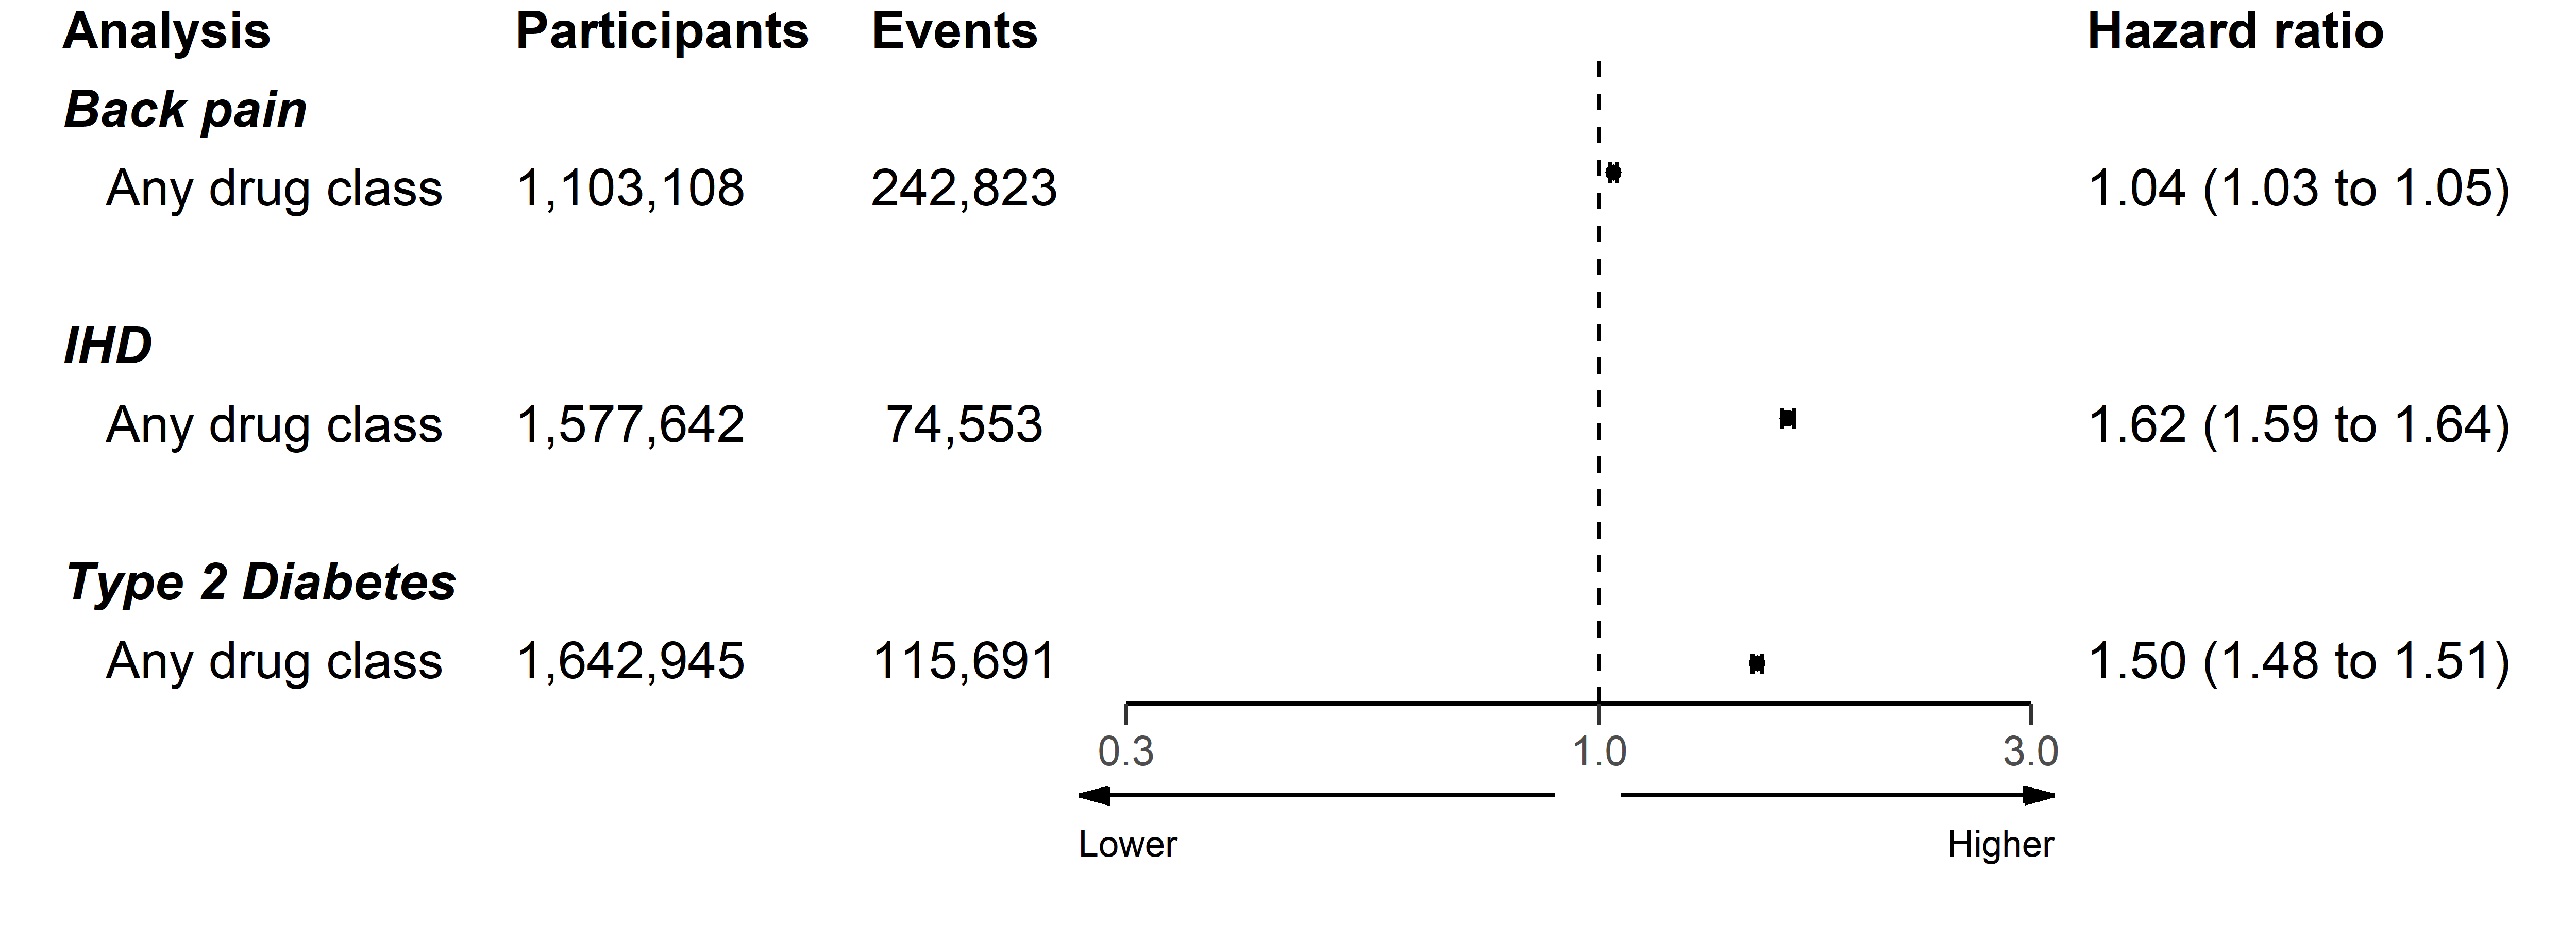
\includegraphics[width=1\linewidth]{figures/cprd-analysis/forester_control_outcomes} \caption[Results of control outcome analysis]{Results of control outcome analysis.}\label{fig:controlOutcomeFig}
\end{figure}

~

\hypertarget{impact-of-additional-covariates-1}{%
\subsubsection{Impact of additional covariates}\label{impact-of-additional-covariates-1}}

The results of three models adjusted for age only, age and sex, and the full covariates respectively, are presented in Figure \ref{fig:unadjustedComparisonFig}. These models were used to estimate the impact of adjustment for additional covariates. Note that obtaining a completely unadjusted model is not possible, as age was used in the Cox model as the time scale.

Adjustment for additional covariates beyond age and sex had a limited impact on the observed effect estimates, with the exception of the probable AD outcome. In this case, adjustment for the full set of covariates attenuated to the null the protective effect observed when adjusting only for age and sex.

~





\begin{figure}[H]
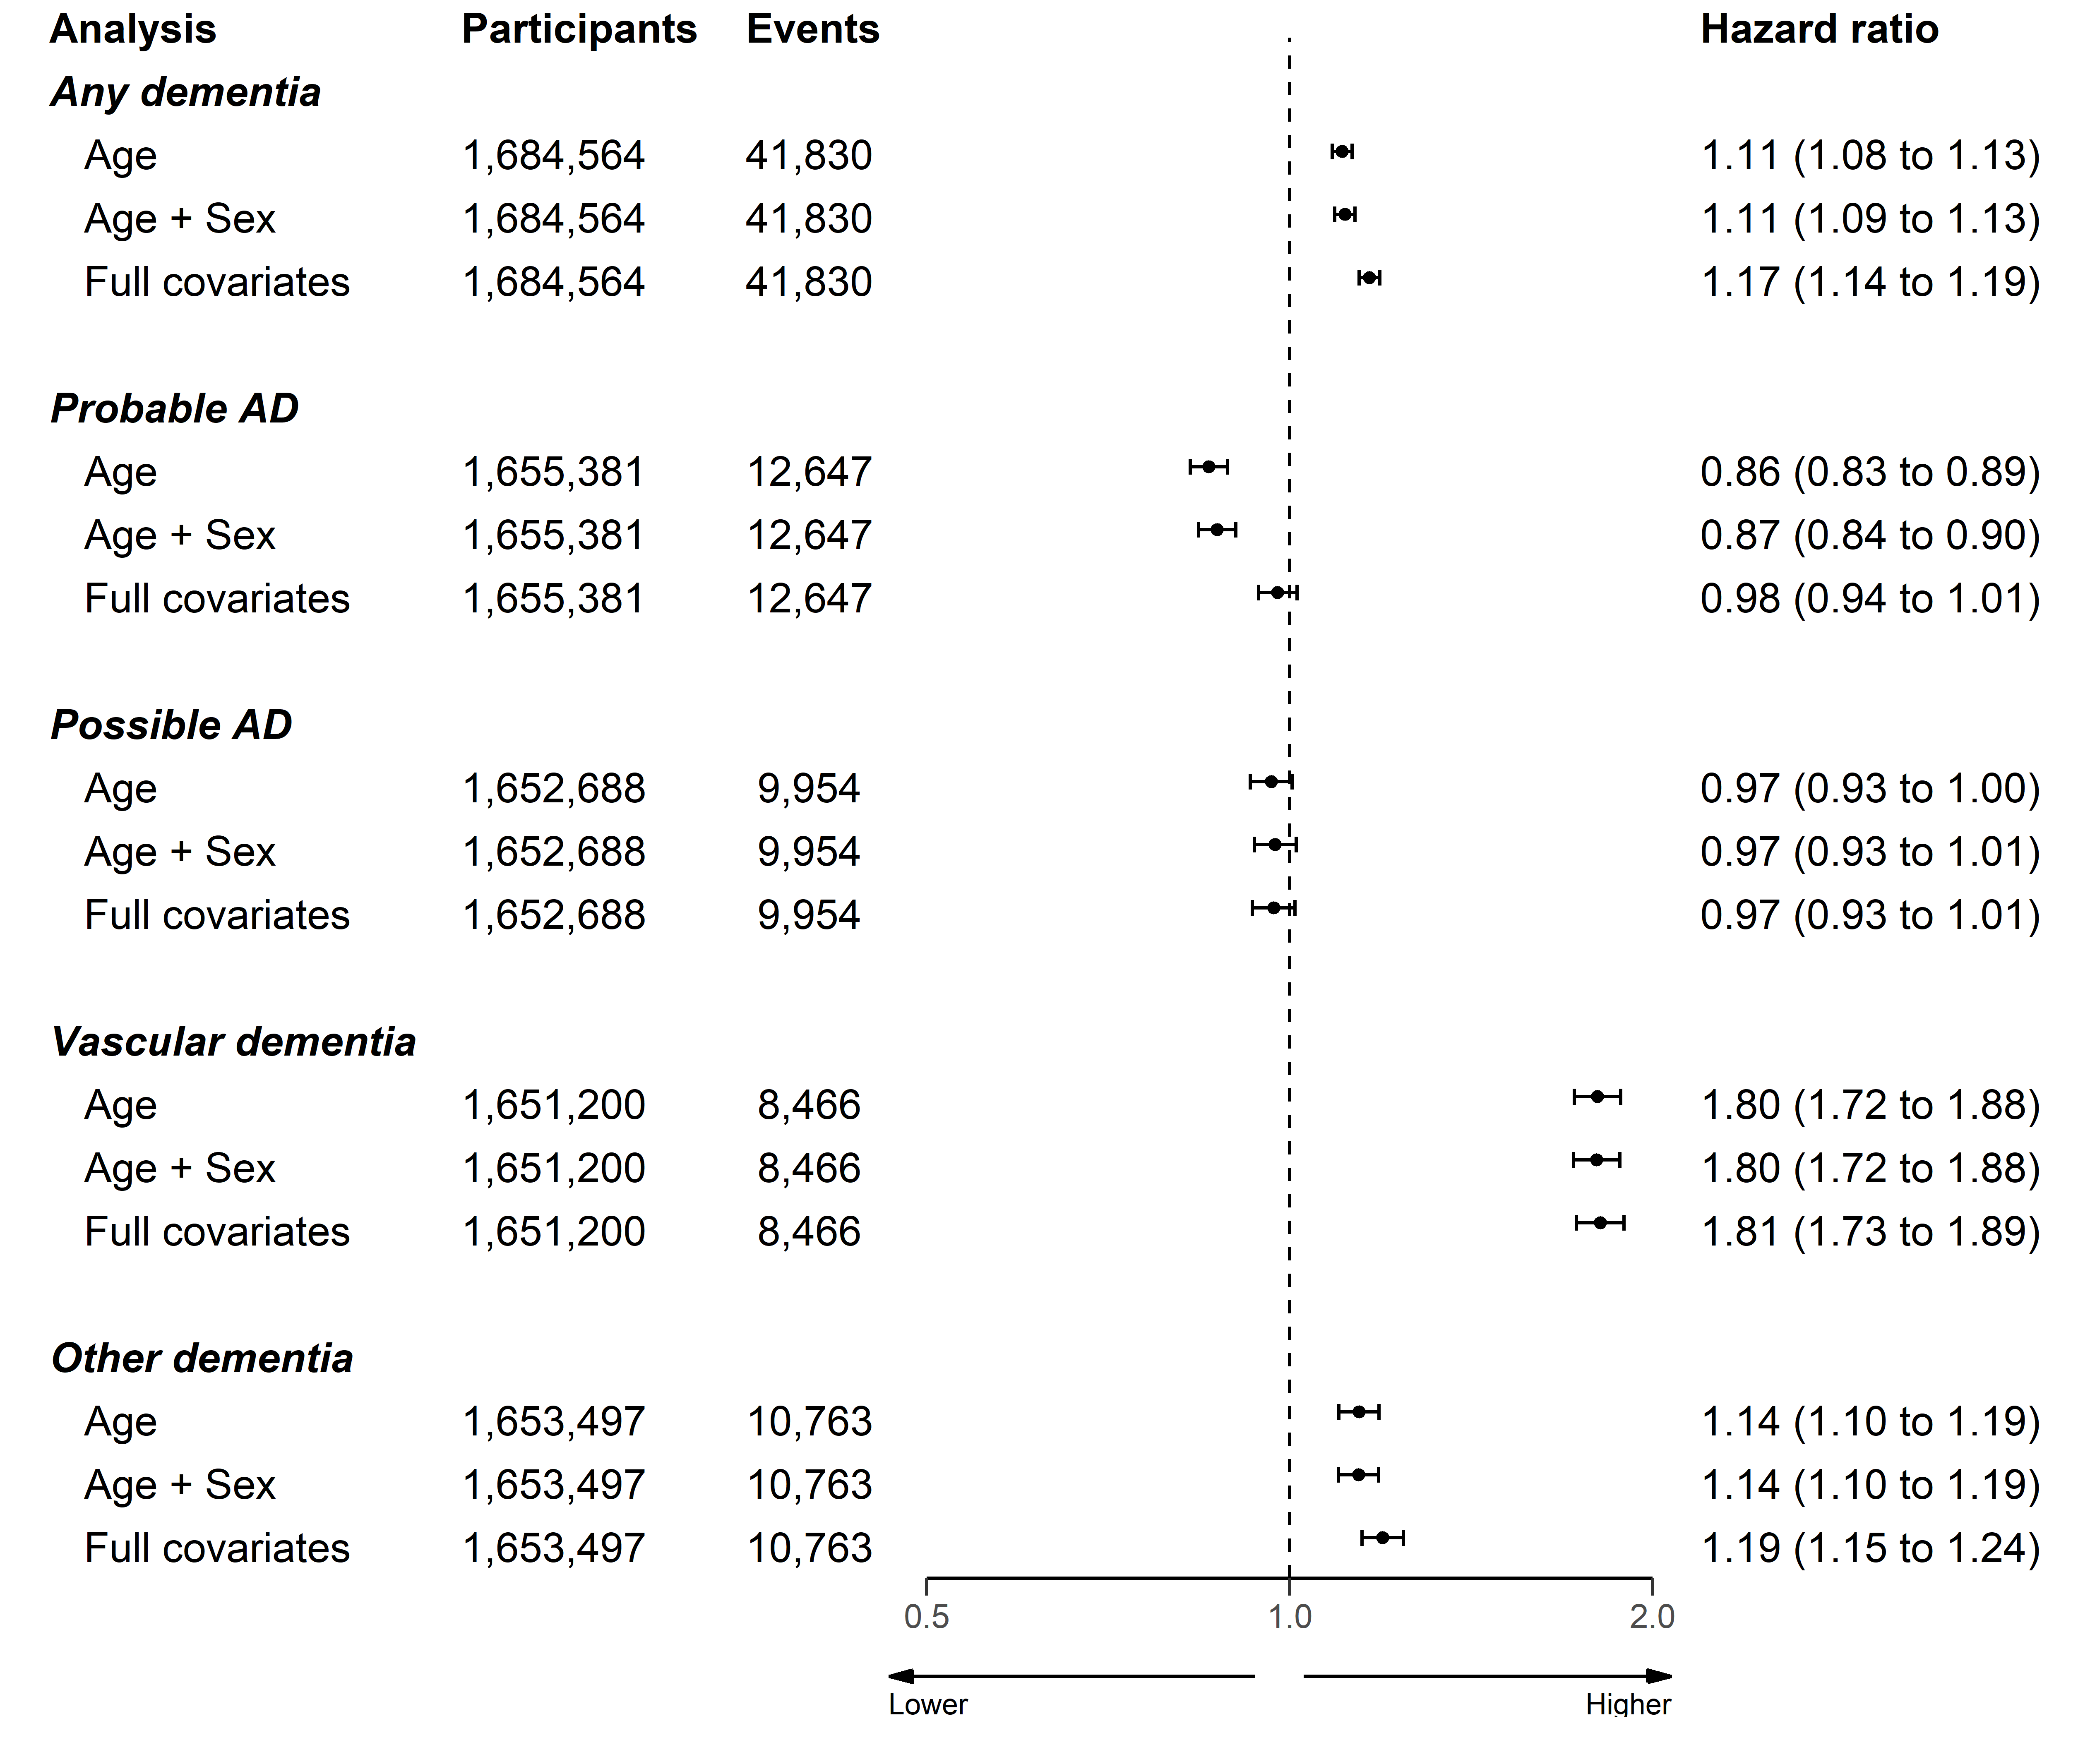
\includegraphics[width=1\linewidth]{figures/cprd-analysis/forester_unadjusted} \caption[Comparison of different combinations of covariates]{Results of three models adjusting for a different set of covariates. Note that the x-axis cutoffs (.5,2) are different compared to other plots (0.3,3) to enable greater comparison between the different models.}\label{fig:unadjustedComparisonFig}
\end{figure}

~

\hypertarget{sensitivity-cohorts-entry-year}{%
\subsubsection{Sensitivity cohorts: Entry year}\label{sensitivity-cohorts-entry-year}}

When stratifying based on year of entry to the cohort, I observed no variation in risk by time period in any subgroup except for probable Alzheimer's disease (Figure \ref{fig:diagnosisTypeFig}).

~





\begin{figure}[H]
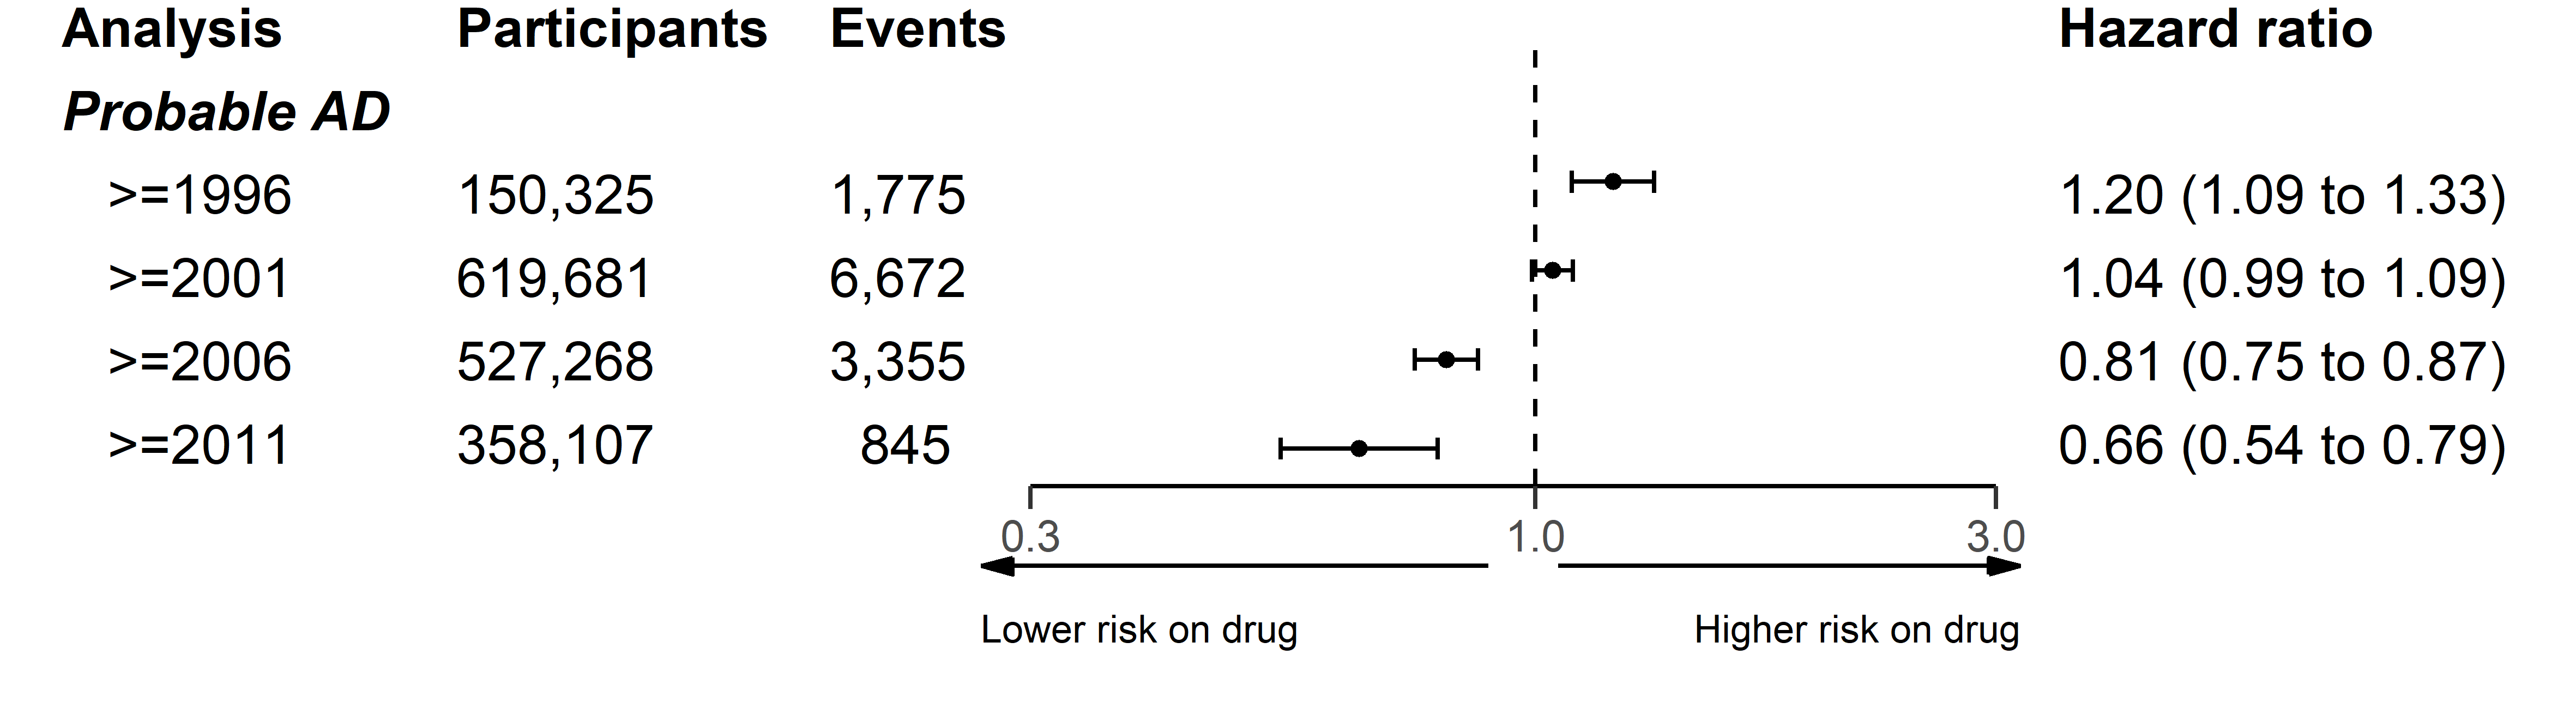
\includegraphics[width=1\linewidth]{figures/cprd-analysis/forester_cohort_entry} \caption[Sensitivity analysis: grouped year of entry]{Analysis of any lipid-regulating agent on probable AD outcome, stratified by grouped year of cohort entry.}\label{fig:diagnosisTypeFig}
\end{figure}

~

On the assumption that this variation could be caused by changes in the frequency probable AD diagnoses in the cohort over time, I performed a \emph{post-hoc} investigation of the frequency of each diagnoses stratified by year of entry (Table \ref{tab:diagnosisType-table}). While the frequency of outcomes declines in more recent strata, likely due to the limited follow-up inherent to these groups, this decline in frequency is relatively constant across the dementia subtypes.

~





\begin{table}[H]

\caption[Frequency of diagnoses by grouped year of cohort entry]{\label{tab:diagnosisType-table}Frequency of diagnoses by grouped year of cohort entry}
\centering
\fontsize{7}{9}\selectfont
\begin{tabular}[t]{>{\raggedright\arraybackslash}p{5.33em}>{\centering\arraybackslash}p{5.33em}>{\centering\arraybackslash}p{5.33em}>{\centering\arraybackslash}p{5.33em}>{\centering\arraybackslash}p{5.33em}>{\centering\arraybackslash}p{5.33em}l}
\toprule
\textbf{\textbf{Year of cohort entry}} & \textbf{\textbf{No dementia}} & \textbf{\textbf{Probable AD}} & \textbf{\textbf{Possible AD}} & \textbf{\textbf{Vascular dementia}} & \textbf{\textbf{Other dementia}} & \textbf{\textbf{Total}}\\
\midrule
<=2000 & 148550 (95.9\%) & 1775 (1.1\%) & 1677 (1.1\%) & 1345 (0.9\%) & 1585 (1.0\%) & 154932\\
\midrule
2001-2005 & 613009 (96.3\%) & 6672 (1.0\%) & 5711 (0.9\%) & 4857 (0.8\%) & 6073 (1.0\%) & 636322\\
\midrule
2006-2010 & 523913 (98.1\%) & 3355 (0.6\%) & 2169 (0.4\%) & 1890 (0.4\%) & 2506 (0.5\%) & 533833\\
\midrule
2010< & 357262 (99.4\%) & 845 (0.2\%) & 397 (0.1\%) & 374 (0.1\%) & 599 (0.2\%) & 359477\\
\midrule
Total & 1642734 (97.5\%) & 12647 (0.8\%) & 9954 (0.6\%) & 8466 (0.5\%) & 10763 (0.6\%) & 1684564\\
\bottomrule
\end{tabular}
\end{table}

~

\hypertarget{sensitivity-cohorts-pregnancy}{%
\subsubsection{Sensitivity cohorts: Pregnancy}\label{sensitivity-cohorts-pregnancy}}

In the second sensitivity cohort, removing participants aged 55 and under at index from the analysis had minimal effect on the effect estimates (Figure \ref{fig:pregnancyFig}).

~





\begin{figure}[H]
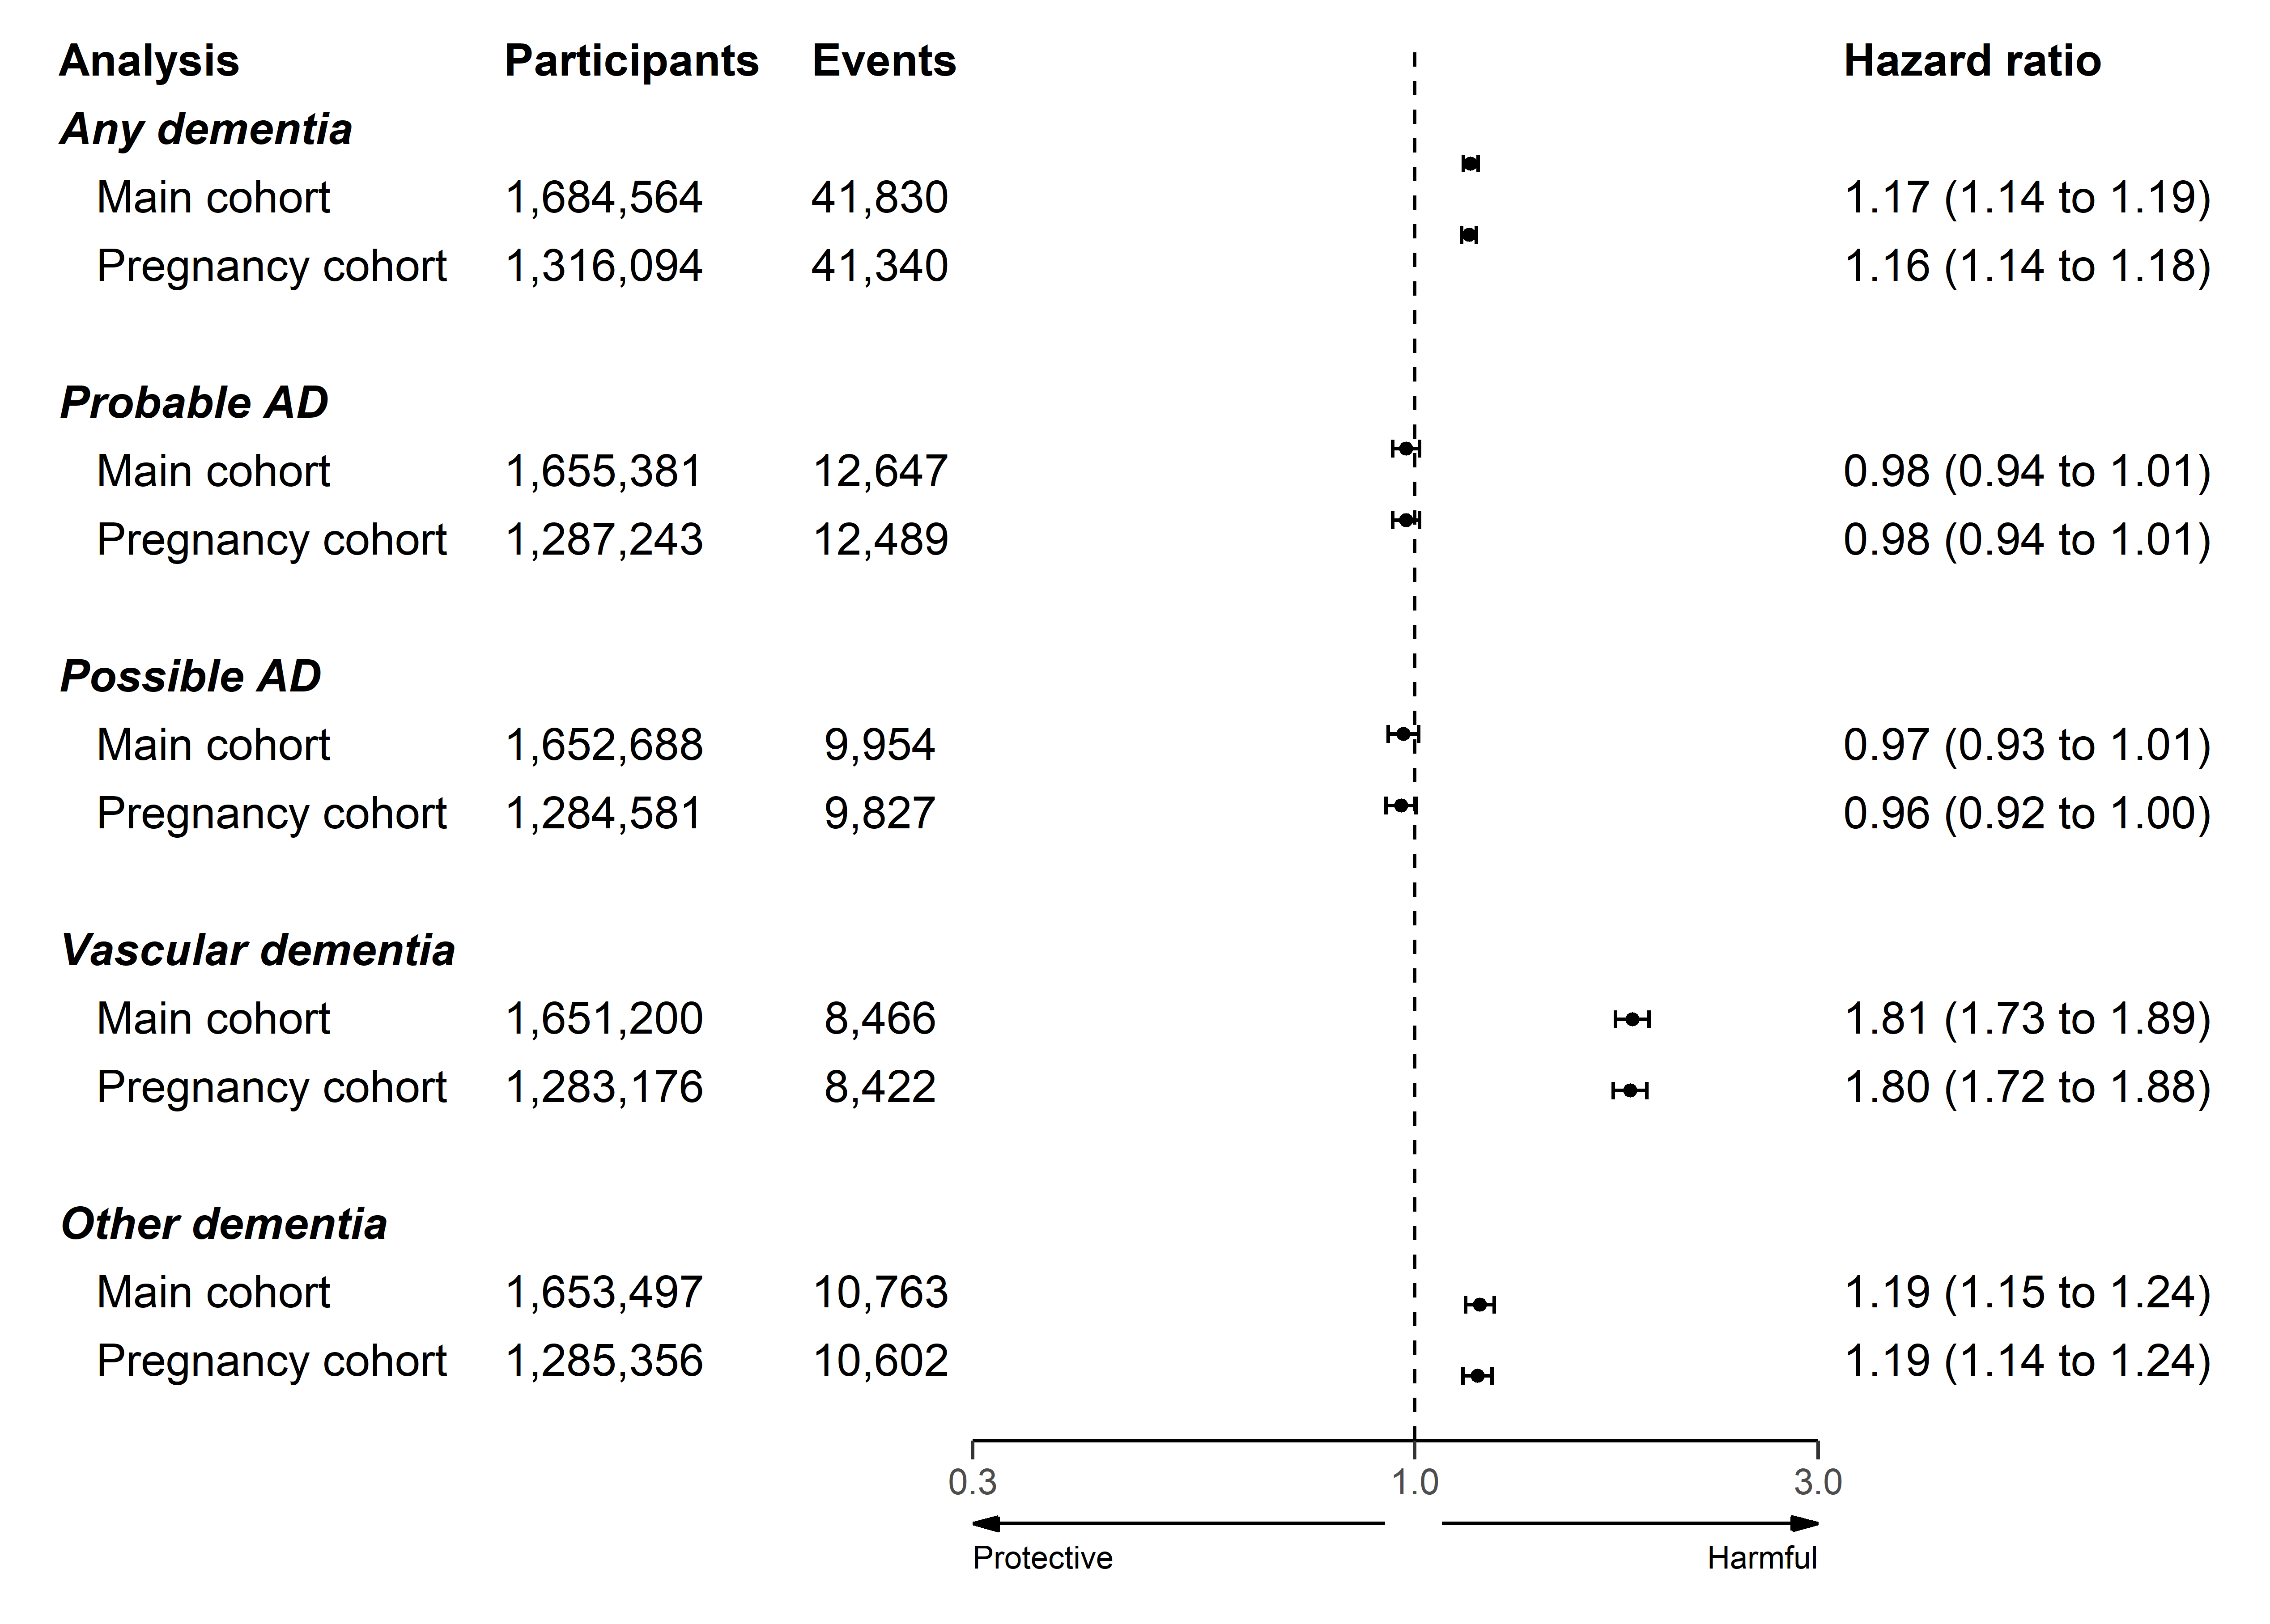
\includegraphics[width=1\linewidth]{figures/cprd-analysis/forester_pregnancy} \caption[Comparison of pregnancy analysis]{Comparison of analysis using main cohort and a cohort with potentially pregnany women removed.}\label{fig:pregnancyFig}
\end{figure}

~

\hypertarget{statin-properties-1}{%
\subsubsection{Statin properties}\label{statin-properties-1}}

In the cohort, statins with lipophilic properties were much more frequently prescribed than hydrophilic statins (Table \ref{tab:statinTypeTable-table}). Additionally, there is evidence for an increasing tendency to favour hydrophilic statins in recent years, as the proportion of lipophilic statins prescribed fell from 18.2\% in 1996-2000 to \textless1\% in 2011-2016.

~





\begin{table}[H]

\caption[Summary of statin properties (lipophilicity vs hydrophilicity).]{\label{tab:statinTypeTable-table}Summary of statin properties (lipophilicity vs hydrophilicity) by grouped year of prescription.}
\centering
\fontsize{7}{9}\selectfont
\begin{tabular}[t]{lccc}
\toprule
\textbf{\textbf{Prescription Year Group}} & \textbf{\textbf{Hydrophilic}} & \textbf{\textbf{Lipophilic}} & \textbf{\textbf{Total}}\\
\midrule
<=2000 & 7037 (18.2\%) & 31531 (81.8\%) & 38568\\
\midrule
2001-2005 & 21427 (10.3\%) & 187018 (89.7\%) & 208445\\
\midrule
2006-2010 & 3566 (1.6\%) & 217726 (98.4\%) & 221292\\
\midrule
2010< & 1115 (0.9\%) & 119035 (99.1\%) & 120150\\
\bottomrule
\end{tabular}
\end{table}

~

When stratifying by statin properties, hydrophilic statins were less harmful in the any, vascular and other dementias outcomes compared to lipophilic statins (Figure \ref{fig:statinTypeFig}). Additionally, in the AD outcomes, hydrophilic statins were associated with a small reduction in risk, compared to the weak evidence for an effect for lipophilic statins.

~





\begin{figure}[H]
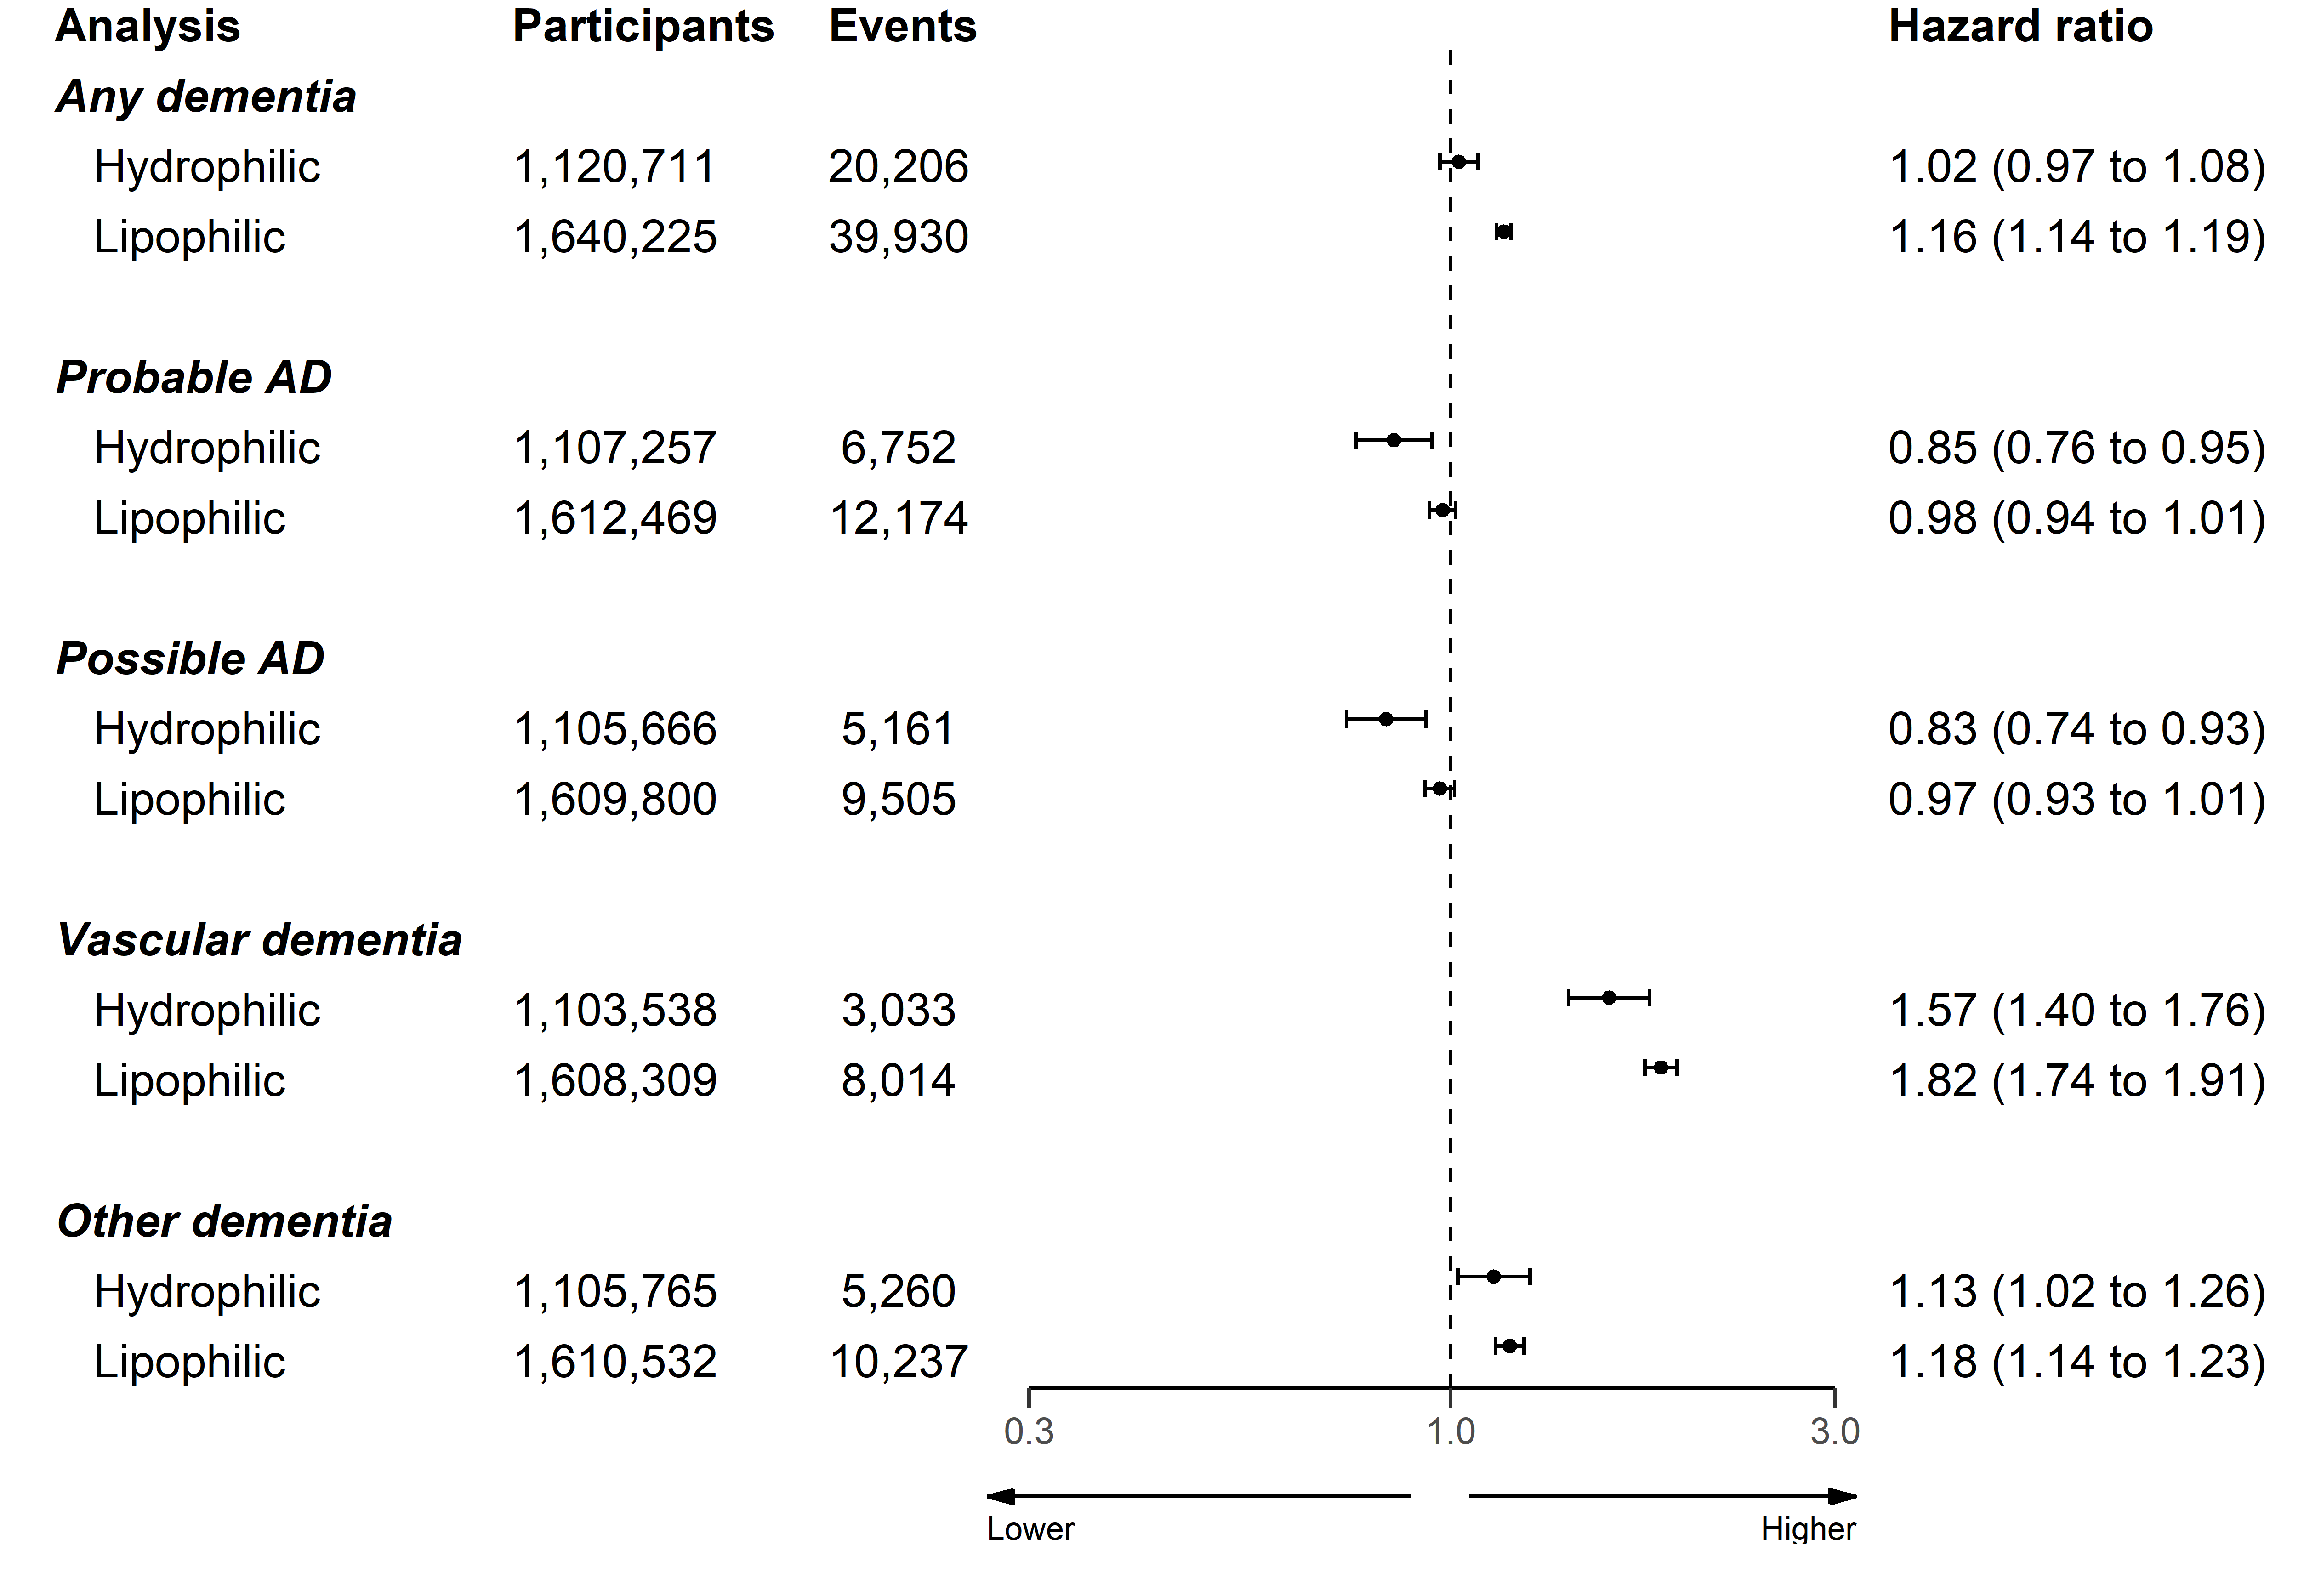
\includegraphics[width=1\linewidth]{figures/cprd-analysis/forester_sta_type} \caption[Analysis stratified by statin properties]{Analysis stratified by statin properties (hydrophilic vs lipophilic)}\label{fig:statinTypeFig}
\end{figure}

~

\hypertarget{impact-of-dementia-code-lists-comparing-code-lists}{%
\subsubsection{Impact of dementia code lists \{\#comparing-code lists\}}\label{impact-of-dementia-code-lists-comparing-code-lists}}

When using the Smeeth \emph{et al.} code lists to define dementia outcomes, effect estimates of HR: 1.19 (95\%CI: 1.07-1.32) and HR: 1.33 (95\%CI: 1.26-1.42) were obtained for the Alzheimer's disease and non-Alzheimer's (``other'') dementia outcomes, respectively. While direct mapping to the outcomes used in this analysis was not possible, the most comparable are probable Alzheimer's disease (HR:0.98, 95\%CI:0.94-1.01) and other dementia (HR:1.19, 95\%CI:1.15-1.24).

~

\hypertarget{discussion-2}{%
\section{Discussion}\label{discussion-2}}

\hypertarget{summary-of-findings-1}{%
\subsection{Summary of findings}\label{summary-of-findings-1}}

Lipid-regulating agents showed little evidence of an association with probable and possible Alzheimer's disease when compared to no treatment, but were associated with increased risk of an all-cause dementia, vascular dementia and other dementias diagnosis. The estimate observed in each case was driven by the statin subgroup, which included a substantial majority of participants. For the other drug classes, no association was found with any outcome, with two exceptions being that ezetimibe was associated with increased risk of vascular and other dementias, while fibrates were associated with increase risk of all-cause dementia and probable Alzheimer's disease.

The effect estimates were robust to the exclusion of potentially pregnant participants, and for all outcomes except probable AD, no variation across grouped year of entry was observed. When looking at the statin subgroup alone, statin properties appeared to have a modifying effect, with hydrophilic statins being less harmful in the any, vascular and other dementias outcomes compared to lipophilic statins.

~

\hypertarget{interpretation-of-results}{%
\subsection{Interpretation of results}\label{interpretation-of-results}}

This section will expand on a potential explanation for the observed results detailed above. However, as the comparison of evidence across different sources is the aim of the triangulation exercise presented in later chapters, the section will not provide a detailed comparison with other published literature, except where needed to illustrate a methodological point. For a detailed comparison of the result presented above with the existing evidence base identified by the systematic review (Chapter \ref{sys-rev-heading}), see Chapter \ref{tri-heading}.

~

\hypertarget{cprd-confounding-by-ind}{%
\subsubsection{Confounding by indication}\label{cprd-confounding-by-ind}}

A likely explanation for the observed increased risk of dementia outcomes with a vascular component (e.g.~vascular and other dementias) with lipid-regulating agent use, and an important limitation of this analysis, is residual ``confounding by indication''. While the term has been used to describe different source of bias in epidemiological analyses,\textsuperscript{\protect\hyperlink{ref-salas1999}{310}} it is used here to described the role of risk factors that both prompt treatment and increase the risk of the outcome, thus causing a distorted positive association between the treatment and outcome (see Figure \ref{fig:indicationBias}). In causal inference nomenclature, statins and dementia are said to be \emph{d}-connected as there is an open ``backdoor'' path between them via the uncontrolled confounders.\textsuperscript{\protect\hyperlink{ref-suttorp2015}{311}} In the context of this analysis, the confounding variable (or, more likely, variables) would prompt both prescription of statins and also represent a vascular risk factor that contributes to the development of the vascular dementia. A similar confounding structure likely exists for ezetimibe, another hypercholesterolemia treatment, providing an explanation for the association of vascular/other dementia but not Alzheimer's disease with this exposure.

~\\




\begin{figure}[H]

{\centering 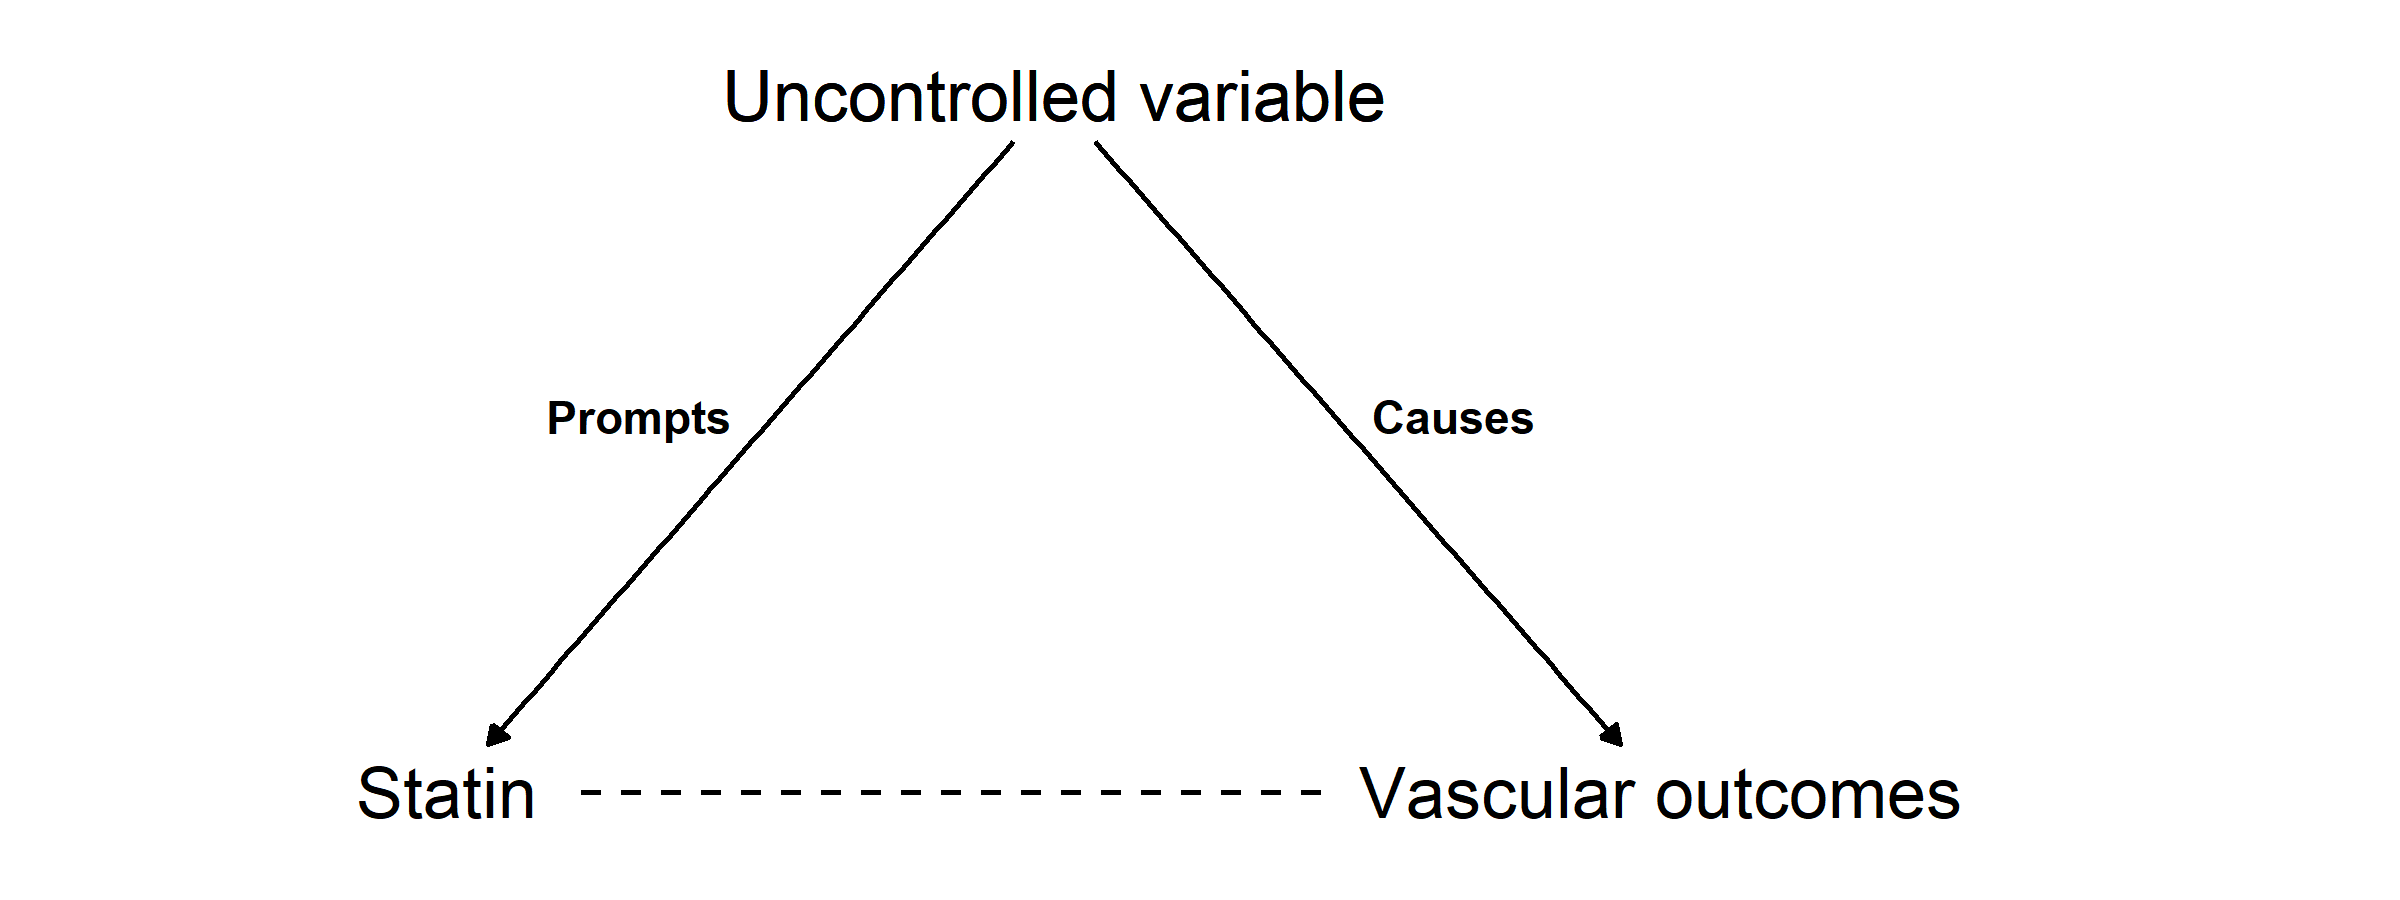
\includegraphics[width=0.8\linewidth]{figures/cprd-analysis/indicationBias} 

}

\caption[Confounding by indication causal diagram]{Causal diagram (directed acyclic graph) illustrating how confounding by indication could induce a positive association between statins and vascular dementia.}\label{fig:indicationBias}
\end{figure}

~

Conditioning entry into the study on being either ``at-risk'' or already diagnosed with hypercholesterolemia was employed in a pre-emptive attempt to mitigate confounding by indication, but evidence from the control outcomes suggests this was unsuccessful. The slight harmful effect for the backpain outcome is substantially smaller than that observed for the ischemic heart disease outcome, indicating that the majority of the uncontrolled confounding is likely related to vascular factors. The slight effect observed for the negative control of backpain could be due to incomplete control for socioeconomic status, as deprivation data was provided in twentiles to preserve patient privacy.\textsuperscript{\protect\hyperlink{ref-boruzs2016}{312},\protect\hyperlink{ref-ikeda2019}{313}}

In line with this, an increasingly harmful effect is observed when moving from the probable and possible Alzheimer's disease outcome to the other dementias outcome, and finally to the vascular dementia outcomes. This pattern suggests that the strength of the residual confounding by indication increases as the proportion of cases with a vascular component in an outcome definition increases. Given confounding related to vascular factors, this pattern is also expected given the decision tree for assigning outcomes in the presence of greater than one dementia code. Under this system, the Alzheimer's disease outcomes require a ``pure'' condition and the presence of any vascular or other dementias codes excludes participants from this group (Figure \ref{fig:decisionTreeFig}).

A review of other available literature suggests that this observation (a harmful effect of lipid-regulating agents on vascular-related outcomes) is not unusual. Using a conventional epidemiological technique, a previous analysis also found an increased risk of coronary heart disease (analogous to the ischemic heart disease outcome used in this analysis) in those taking statins (HR: 1.31, 95\%CI: 1.04-1.66).\textsuperscript{\protect\hyperlink{ref-danaei2013}{314}} Controlling for confounding by indication in that study through the use of a trial emulation analysis gave an estimate of 0.89 (95\%CI: 0.73-1.09), a comparable though less precise estimate to that observed in RCTs of statin use (0.73, 95\%CI: 0.67-0.80).\textsuperscript{\protect\hyperlink{ref-taylor2013}{315}}

Given the absence of vascular dementia in the published literature, as highlighted in the previous chapter (see Section \ref{sys-rev-pub-bias}), the unexpected increase in vascular dementia risk with statin use is particularly interesting. It is possible that this finding reflects publication bias if previous research encountered similar methodological issues to this analysis, and these results did not make it into the evidence base as unexpected or assumedly incorrect results are less likely to be submitted or accepted for publication.

~

\hypertarget{statin-properties-2}{%
\subsubsection{Statin properties}\label{statin-properties-2}}

This analysis found that hydrophilic statins were less harmful in the any, vascular and other dementias outcomes compared to lipophilic statins, and were associated with a small reduction in the risk of the probable and possible AD outcomes. The relative precision of the estimates in each group is expected, as the two most commonly prescribed statins are lipophilic (simvastatin and atorvastatin).\textsuperscript{\protect\hyperlink{ref-newman2019}{316}}

A widely discussed concept in the literature surrounding statin use and cognitive outcomes is the fact that lipophilic statins are more likely to be able to cross the blood brain barrier, and so have a more potent protective effect by directly lowering brain cholesterol.\textsuperscript{\protect\hyperlink{ref-shepardson2011}{317}} My findings that hydrophilic statins appear to be more protective/less harmful than their lipophilic counterparts runs counter to this assertion.

An initial interpretation of the different associations observed in the two groups was that the lipophilic statins may be more potent, and so are prescribed to patients with a higher underlying vascular load, leading to increased confounding by indication in this group. However, the statin with the strongest lipid lowering effect that is available via the NHS, rosuvastatin, is hydrophobic.

~

\hypertarget{impact-of-code-lists}{%
\subsubsection{Impact of code lists}\label{impact-of-code-lists}}

As part of a sensitivity analysis exploring the impact of outcome code-lists, I used definitions for Alzheimer's disease and other dementias obtained from a previously published paper (Smeeth \emph{et al.}).\textsuperscript{\protect\hyperlink{ref-smeeth2009}{210}} Using these lists in my analytical set-up, I found a harmful association of statin use with both outcomes.

This finding disagrees with the results of the original analysis, which found evidence for a protective effect of statin use on all-cause dementia (HR: 0.81, 95\%CI: 0.69-0.96) and non-AD dementia (HR: 0.82, 95\%CI: 0.69-0.97), but little evidence of an effect on AD (HR: 0.81, 95\%CI: 0.49-1.35).

However, comparison of the results obtained using the two sets of code lists was deemed less useful following a detailed comparison of the codes used. While all of the codes used to define Alzheimer's in the Smeeth \emph{et al.} paper are included in the probable Alzheimer's code-list (see Figure \ref{fig:smeethComparison}), I included several additional codes used to define this outcome (including, for example, ``Eu00013: {[}X{]}AD disease type 2''). Additionally, several of the codes used to define ``Possible Alzheimer's'' in this analysis are included in the ``Other dementia'' code list used by Smeeth.

~





\begin{figure}[H]
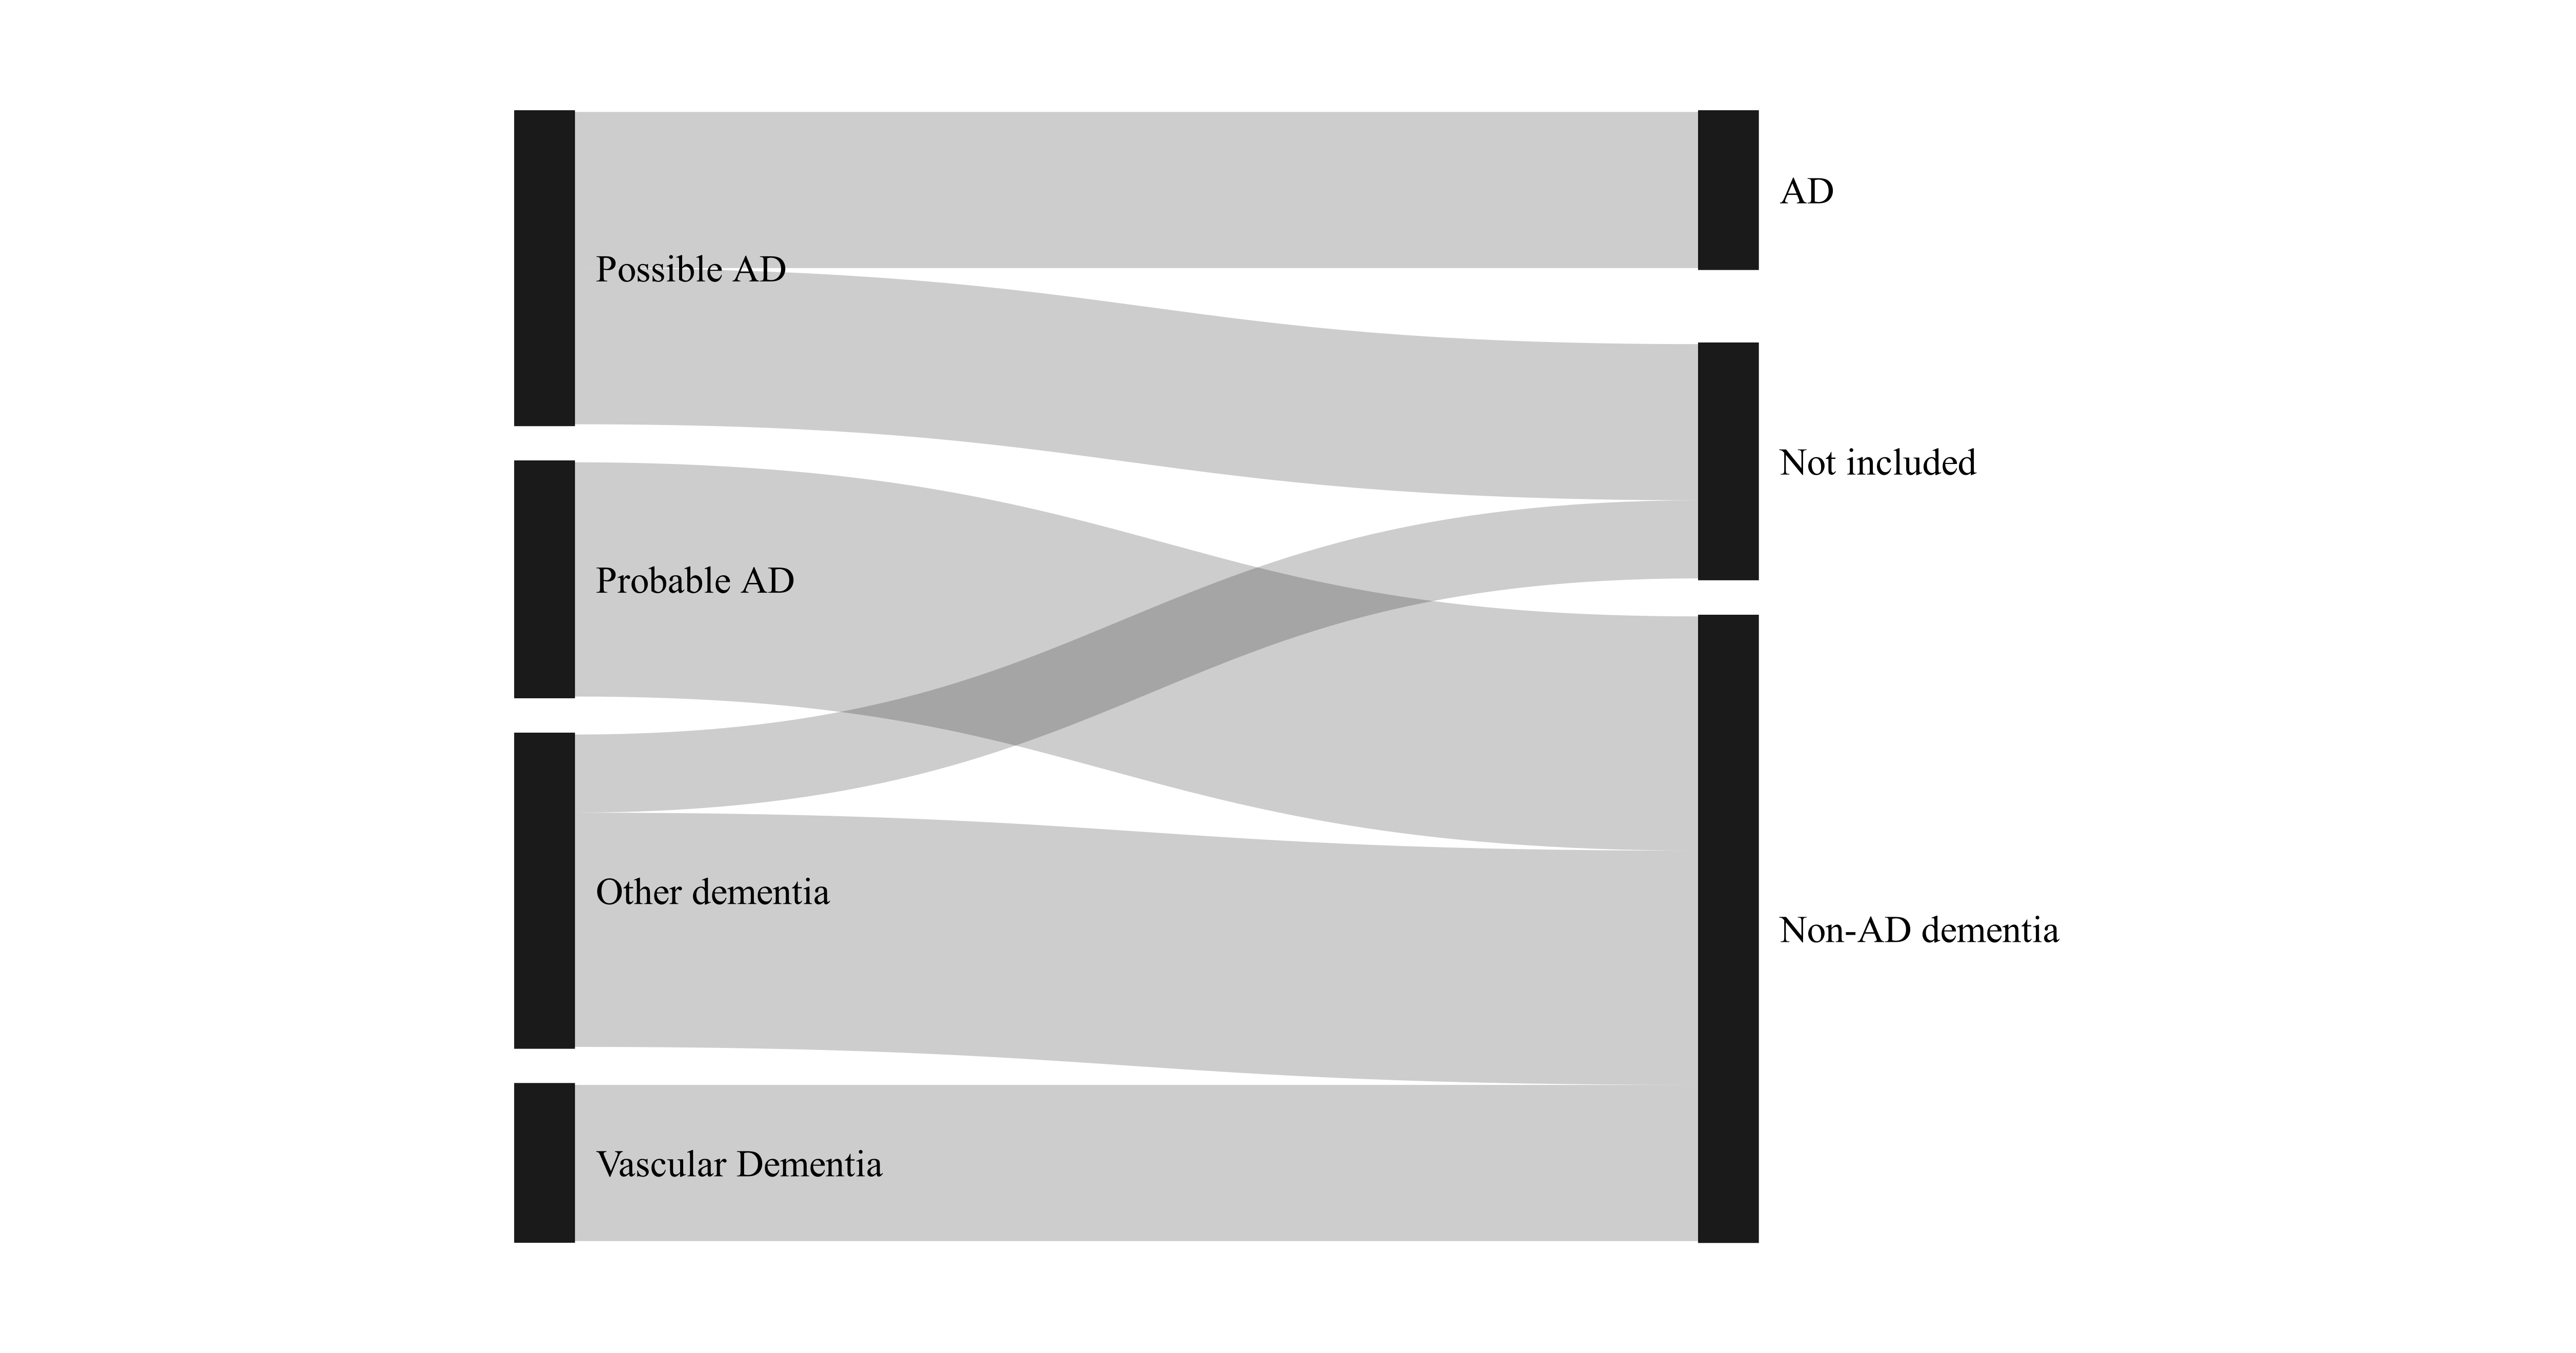
\includegraphics[width=1\linewidth]{figures/cprd-analysis/sankey_diagram} \caption[Comparison of code used in this analysis with those used in the Smeeth et al.~2010 paper]{Sankey diagram comparing the codes used in this analysis with those used in the Smeeth \emph{et al} paper.\textsuperscript{\protect\hyperlink{ref-smeeth2009}{210}} The outcomes and number of codes contributing to each are presented (the Smeeth \emph{et al} outcomes are on the right hand side of the figure). The joining lines showing the overlap between the categories in the two analyses.}\label{fig:smeethComparison}
\end{figure}

This analysis serves to illustrative the importance of the code lists chosen to define the outcomes of interest, particularly if they are used to define competing outcomes (e.g.~AD vs non-AD dementia). This different codes used by Smeeth \emph{et al.}, in addition to an analytical approach that adjusted for covariates defined after the index date, may go some way to explaining why our analysis obtained different results despite the substantial overlap in the data sources used.

~

\hypertarget{cprd-limitations}{%
\subsection{Strengths and limitations}\label{cprd-limitations}}

The primary strength of this analysis is the relative size of the CPRD and length of follow-up. Having reviewed the existing literature, as identified by the systematic review in Chapter \ref{sys-rev-heading}, this analysis of 1,684,564 participants is one of the largest available studies of this research question. Additionally, this analysis followed LRA users and non-users from a common index date, using a time-updating treatment indicator to correctly assign time-at-risk to the exposed and unexposed groups. This approach has been less commonly used in the literature and allows for the mitigation of potential immortal time bias. Finally, it is one of the few that provide evidence on the association of lipid-regulating agent use and vascular and other dementias, and used negative and positive controls to assess the potential for residual confounding.

However, the findings of this analysis are subject to several limitations in addition to the confounding by indication discussed above. There is a strong possibility of differential misclassification of dementia-related conditions based on the exposure.\textsuperscript{\protect\hyperlink{ref-porta2014}{318}} As an illustrative example, those with memory complaints may be more likely to be classified as vascular dementia than Alzheimer's disease if their medical records contain prescriptions for lipid-regulating agents. Further, there is a potential for general non-differential misclassification of the outcome due to the varying positive predictive value of electronic health record code lists to identify dementia cases.\textsuperscript{\protect\hyperlink{ref-mcguinness2019validity}{275},\protect\hyperlink{ref-wilkinson2018}{276}}

Misclassification of outcomes is not the only issue introduced by the use of EHR codes to define outcomes. Comparing and contrasting between different studies is particularly difficult because of the impact that the use of different code lists can have on the analysis, as illustrated by the discrepancy between the results when using the code lists defined for this study and those used by Smeeth \emph{et al}. This presents a particular challenge in comparing research across different time-periods and coding systems, particularly the unexpected results I obtained for the vascular and other dementias outcomes.

A further limitation stems from the possibility of uncontrolled confounding due to genetic factors. The number of ApoE \(\epsilon4\) alleles represents the strongest genetic risk factor for Alzheimer's disease, but also substantially increases LDL cholesterol levels,\textsuperscript{\protect\hyperlink{ref-bennet2007}{319}} potentially prompting treatment with a statin or other lipid regulating agent. I was unable to control for ApoE genotype in this analysis as I did not have access to genetic data on participants. As a result, any protective association between LRA use and the Alzheimer's disease outcomes may be masked by residual negative confounding by ApoE.

Finally, as with many studies of dementia, there is a risk of reverse causation in my analysis. Dementia and associated conditions have a long prodromal period, during which preclinical disease could cause indications for the prescription of a lipid-regulating agent.

~

\hypertarget{cprd-data-avail}{%
\subsection{Enabling easy synthesis of this analysis}\label{cprd-data-avail}}

The raw data supporting this analysis is not publicly available, as access to the CPRD data is controlled by a data monitoring committee. However, when data are not readily available, sharing the analysis code and summary statistics represents a way for readers to validate the findings.\textsuperscript{\protect\hyperlink{ref-goldacre2019}{137}}

In light of this and my own experiences in attempting to extract information for papers assessing preventative treatments, as documented in Section \ref{sys-rev-open-data}, the outputs from this analysis have been made readily available. All code, Read code lists and summary statistics (namely the tables presented in this chapter plus summary tables of effect estimates) can be downloaded in a machine readable format from the archived repository for this project (Zotero DOI: \textbf{TBC}). This open approach should enable easy inclusion of this analysis in future evidence synthesis exercises, allowing new work to build on that presented here.

~

\hypertarget{summary-4}{%
\subsection{Summary}\label{summary-4}}

\begin{itemize}
\item
  In this chapter, I produced new evidence on the association of lipid-regulating agents with incidence of all-cause dementia, Alzheimer's disease, vascular dementia, and other dementia.
\item
  I found little evidence for an effect of lipid-regulating agents on probable or possible Alzheimer's disease. However, lipid-regulating agent use was associated with an increased risk of all-cause, vascular and other dementias. In all cases, the estimated associations were driven by those observed in the large statin subgroup.
\item
  I attempted to account for important sources of bias through use of time-varying treatment indicator, though the control outcomes included in the analysis provided evidence for only partially controlled confounding by indication related to vascular factors. Additionally, there was the potential for differential misclassification of dementia subtype on the basis of the exposure. Combined, these biases reduce the confidence in my findings, in particular the unexpected increase in risk of vascular dementia associated with statin use.
\item
  Findings from this analysis are used as an additional source of evidence in the triangulation exercise presented in Chapter \ref{discussion-heading}.
\end{itemize}

\newpage

\hypertarget{references-4}{%
\section{References}\label{references-4}}



\hypertarget{ipd-heading}{%
\chapter{Individual participant data meta-analysis of blood lipid levels and dementia outcomes}\label{ipd-heading}}

\minitoc 

\hypertarget{lay-summary-5}{%
\section{Lay Summary}\label{lay-summary-5}}

TBC

~

\hypertarget{introduction-3}{%
\section{Introduction}\label{introduction-3}}

Individual patient data (IPD) meta-analyses are considered to be the gold standard form of evidence synthesis, allowing for the application of a common selection model and analytical approach across all identified cohorts.\textsuperscript{\protect\hyperlink{ref-riley2010}{95}} They are particularly useful for investigating the impact of patient-level characteristics, something that is not possible with aggregate data unless the results are stratified by the characteristic of interest.\textsuperscript{\protect\hyperlink{ref-riley2010}{95},\protect\hyperlink{ref-thompson2005}{320}} Knowledge of which groups a treatment will benefit most (or harm least) is a core aim of the move towards personalised medicine.\textsuperscript{\protect\hyperlink{ref-riley2020}{101},\protect\hyperlink{ref-hingorani2013}{321}}
IPD analysis also offer a mechanism by which previously unanalysed datasets can be incorporated into an analysis, thus expanding the evidence base for a particular research question.

Previous work has suggested a difference in the effect of lipids on dementia risk based on patient age and sex.\textsuperscript{\protect\hyperlink{ref-mielke2010}{58},\protect\hyperlink{ref-ancelin2013}{217}} While the systematic review presented in Chapter \ref{sys-rev-heading} did not identify strong evidence for an effect of sex or age at lipid measurement on the relationship between lipids and dementia. However, the number of included studies in the lipid fraction meta-analyses was small, due to both the relatively small number of studies reporting on the lipids exposure and the poor reporting of summary statistics of patient characteristics in those that did. Additionally, best practice guidance recommends against basing the decision to perform an IPD meta-analysis on the between-study heterogeneity in a summary data meta-analysis, as similar distributions of patient covariates across studies may mask a true effect.\textsuperscript{\protect\hyperlink{ref-riley2020}{101}}

As such, the aims of this analysis are two fold: firstly, to perform a individual patient data meta-analysis across identified cohorts to examine the impact of patient age-at-measurement and sex on the effect of lipids on dementia risk; and secondly, to expand the evidence base for the effect of lipids on dementia outcomes by obtaining estimates from previously unanalysed cohorts available via the Dementia Platform UK, a large consortia of dementia cohorts.

~

\hypertarget{methods-2}{%
\section{Methods}\label{methods-2}}

\hypertarget{eligibility-criteria-1}{%
\subsection{Eligibility criteria}\label{eligibility-criteria-1}}

\hypertarget{study-design}{%
\subsubsection{Study design}\label{study-design}}

Data sources which were cross-sectional, either by design or due to the available data (e.g.~a study conducted across multiple waves, but only data from a single wave could be accessed) were excluded. Similarly, due to the limited time afforded by this thesis, studies making use of population-level electronic health records, which often require an extensive project proposals in order to gain access to the data, were ineligible due to the time and cost involved in applying. No restrictions were put on the number of participants or the length of follow-up, though participants must be free of dementia (or assumed to be free, based on age at entry) at baseline.

~

\hypertarget{exposuresoutcome-definition}{%
\subsubsection{Exposures/outcome definition}\label{exposuresoutcome-definition}}

I considered four blood lipid fractions as part of this analysis, namely: total cholesterol (TC), low-density lipoprotein cholesterol (LDL-c), high-density lipoprotein cholesterol (HDL-c) and triglycerides (TG). Cohorts were eligible for inclusion if they contained data on at least one of these in a continuous format (i.e.~studies with binary ``hypercholesteromemia'' would be excluded).

In line with the analyses presented in other chapters, eligible cohorts were those containing data on at least one outcome of interest, namely: all-cause dementia, Alzheimer's disease, or vascular dementia.

~

\hypertarget{applying-for-data-access}{%
\subsection{Applying for data access}\label{applying-for-data-access}}

Potentially eligible data sources as defined above were identified via two mechanisms, each with a distinct focus. For both approaches, the number of cohorts responding to the request for data access, and where applicable, the reasons given for a lack of data sharing were recorded.

~

\hypertarget{cohorts-identified-by-the-systematic-review}{%
\subsubsection{Cohorts identified by the systematic review}\label{cohorts-identified-by-the-systematic-review}}

The first approach focused on previously analysed observational prospective cohort studies examining the effect of blood lipid levels on dementia outcomes, as identified by the systematic review presented in Chapter \ref{sys-rev-heading} The data sources used in each of these cohort analyses were screened against the criteria listed in the previous section, and eligible cohorts were approached for data access. In the first instance, the first/corresponding author of the publication was emailed (see Appendix \ref{ipd-email-collab} for a copy of the text and documentation sent to potentially collaborators) in Autumn 2020. If this approach did not elicit a response within two months, the last author was contacted, on the basis that the first/corresponding author may have been a more junior member of the research group who has moved to a different institution.

~

\hypertarget{cohorts-contained-in-dementia-platform-uk}{%
\subsubsection{Cohorts contained in Dementia Platform UK}\label{cohorts-contained-in-dementia-platform-uk}}

The second approach focused on incorporating relevant, previously-unanalysed data into the analysis, thus providing additional evidence on the relationship between blood lipids and dementia risk. This was achieved through the Dementia Platform UK (DPUK), a collaborative grouping of existing dementia cohorts established by the MRC which works with data owners to make their data readily accessible for secondary analysis.\textsuperscript{\protect\hyperlink{ref-bauermeister2020}{111}} It provides access to 42 cohorts with over 3 million participants, and makes use of a central streamlined application processs for all cohorts with the intent of making it easier to access data from existing data sources.

Cohorts included in the DPUK were assessed against the eligibility criteria, and in Autumn 2020, an application for access to a subset of 17 cohorts was made via the common-access procedure.

~

\hypertarget{primary-analysis-1}{%
\subsection{Primary analysis}\label{primary-analysis-1}}

\hypertarget{data-cleaning-and-harmonisation}{%
\subsubsection{Data cleaning and harmonisation}\label{data-cleaning-and-harmonisation}}

Where data on one of these exposures (TC, LDL-c, HDL-c, TG) was missing, it was inferred from the other three fractions (where available) using the Friedwald formula (Equation \eqref{eq:total-cholesterol-formula}). Lipids levels were retained as continuous variables rather than dichotomising into a binary hypercholesterolemia exposure, given the additional power this adds to the meta-analysis.\textsuperscript{\protect\hyperlink{ref-riley2020}{101},\protect\hyperlink{ref-ensor2018}{322}} Where lipid measurements were reported in \emph{mg/dL}, these were converted to \emph{mmol/L}. To aid interpretability of the outcome, all analyses were standardised to refer to a 1-standard deviation increase in the lipid fraction under investigation.

Across all cohorts, data cleaning was performed in a similar manner, standardising to commonly named variables so that a single model could be applied using functional programming.\textsuperscript{\protect\hyperlink{ref-wickham2016func}{323}} The advantage of this approach is that it reduces the likelihood of errors in model mis-specification if needing to change variables names from cohort to cohort. Following data cleaning, summary statistics for each data source were calculated and compared to publicly available statistics to ensure no errors were introduced in the data cleaning process, in line with best practice.\textsuperscript{\protect\hyperlink{ref-levis2021}{324}}

~

\hypertarget{covariate-definition}{%
\subsubsection{Covariate definition}\label{covariate-definition}}

With an awareness that discrepancies in available covariates is a common issue in IPD studies, I defined an idealised set of covariate domains to be age, sex, education, BMI, ApoE4 status, smoking/alcohol status and prevalent cardiovascular disease. This set covers key risk factors for dementia/Alzheimer's disease in addition to general cardiovascular risk factors. Ethnicity was considered as a potential addition covariate of interest, but several of the DPUK cohorts (whose data dictionaries could be inspected in advance) made it clear that ethnicity data was either not available or would not be shared. Details on how these variables were coded, given the available data, are presented in Section \ref{ipd-covar-definition}.

~

\hypertarget{missing-data-2}{%
\subsubsection{Missing data}\label{missing-data-2}}

Missing data in this analysis was classified as either relating to missing values (a cohort collected data on a variable of interest, but some values are missing) or missing variables (a cohort did not collect data on a variable of interest).

Variables with missing values were identified, and 20 imputed datasets were created.\textsuperscript{\protect\hyperlink{ref-sterne2009}{295}} Imputation was performed using the MICE (Multiple Imputation by Chained Equations) using the \texttt{mice} package in R.

Systematically missing variables were originally intended to be addressed using a previously described method.\textsuperscript{\protect\hyperlink{ref-fibrinogenstudiescollaboration2009}{325}} Here, the correlation between the fully-adjusted and partially-adjusted estimate in cohorts with the full set of covariates is used to estimate the fully-adjusted effect in those cohorts missing covariates. However, this method requires several large cohorts to contain the full set of covariates, a condition this analysis failed to meet given the very low response rate. As such, two other common approaches were employed.\textsuperscript{\protect\hyperlink{ref-fibrinogenstudiescollaboration2009}{325}} In the primary analysis, all cohorts were analysed adjusted for the set of common covariates across cohorts (Model 1: age, sex, smoking, alcohol, presence of morbidities). As a sensitivity analysis, cohorts with the full complement of covariates (Whitehall II and EPIC) were analysed using a maximally-adjusted model (Model 2: Model 1, further adjusted for education and BMI). Results between the common-set-adjusted (Model 1) and maximally-adjusted (Model 2) models were then compared.

~

\hypertarget{individual-patient-data-analysis}{%
\subsubsection{Individual patient data analysis}\label{individual-patient-data-analysis}}

In this analysis, an two-stage individual patient data analysis was planned. Under a two-stage approach, estimates for the effect of each lipid fraction on available dementia outcomes were first calculated for each data source. More specifically, odds ratios were used to quantify the effect of a 1-SD lower exposure to a lipid fraction on dementia outcomes. Examination of the data available via the DPUK indicated that the common time-to-event approach used in studies of dementia outcomes would be precluded by the absence of detailed time-to-event data. An overall effect estimate was then produced by combining data-source-specific estimates in a random-effects meta-analysis (see Section \ref{hold} in Chapter \ref{hold} for a broader discussion of meta-analysis methods).

A two-stage IPD approach was employed for a number of reasons. Firstly, and most importantly, a two-stage approach allows for siloed data, enabling researchers who are unwilling/unable to provide their data to analyse themselves following a specified analysis plan.\textsuperscript{\protect\hyperlink{ref-riley2010}{95}} Secondly, it allows for the production of forest plots of within-cohort estimates, something which is useful for the triangulation exercise in Chapter \ref{tri-heading}. Finally, a two-stage approach is simpler to model, as it uses standard well-documented summary effect estimate meta-analysis techniques, and automatically accounts for methodological issues such as clustering within cohorts\textsuperscript{\protect\hyperlink{ref-abo-zaid2013}{326}} and the potential for ecological bias.\textsuperscript{\protect\hyperlink{ref-burke2017}{327}}

~

\hypertarget{comparison-with-published-findings}{%
\subsubsection{Comparison with published findings}\label{comparison-with-published-findings}}

Following estimation of the main effect, where an included data source had previously been analysed, the results of this analysis were compared against those published previously. Where discrepancies were identified, these were investigated.

~

\hypertarget{investigating-the-effect-of-patient-level-covariates}{%
\subsubsection{Investigating the effect of patient-level covariates}\label{investigating-the-effect-of-patient-level-covariates}}

In order to investigate the interaction of patient-level characteristics (age and sex) with lipid levels, interaction terms for lipid-covariate terms were extracted and synthesised using a random effects meta-analysis.\textsuperscript{\protect\hyperlink{ref-fisher2017}{328}} To avoid ecological bias, where the between-study association does not reflect the within-study associations, cohorts where there was no within-study variation in the covariate of interest were excluded from the interaction analysis for that covariate.\textsuperscript{\protect\hyperlink{ref-burke2017}{327}} As an example, it is impossible to estimate the impact of sex on the lipid\textasciitilde dementia relationship in a study which contains female participants. All interaction analysis were performed using the common-set-adjusted model (Model 1).

~

\hypertarget{results-2}{%
\section{Results}\label{results-2}}

\hypertarget{data-access}{%
\subsection{Data access}\label{data-access}}

Of the 37 studies to which I applied for data access, only three (8.1\%) were included in the final analysis. Figure \ref{fig:cohortFlowchart} details whether the cohorts eventually included in the review were identified by the systematic review or via DPUK portal. In addition, the reasons for cohorts not being included in the analysis are presented, where available, stratified by application approach.

In summary, the requests for data from cohorts identified by the systematic review were characterised by a very low response rate. For the minority who did respond, common reasons given by authors for not sharing the data included that they: no longer worked with the same group and did not know if the data were available or how to obtain it; no longer had access to the data; or were currently performing, or intended to perform, a similar analysis as the one proposed.

With respect to the application to DPUK cohorts, where a dedicated project manager liaises with data owners on the applicants' behalf, the overall response rate was higher. However, even using this streamlined approach, a response was obtained for approximately half (N=9, 53\%) of the approached cohorts, one of which (Whitehall II) was also identified by the systematic review.





\begin{figure}[H]
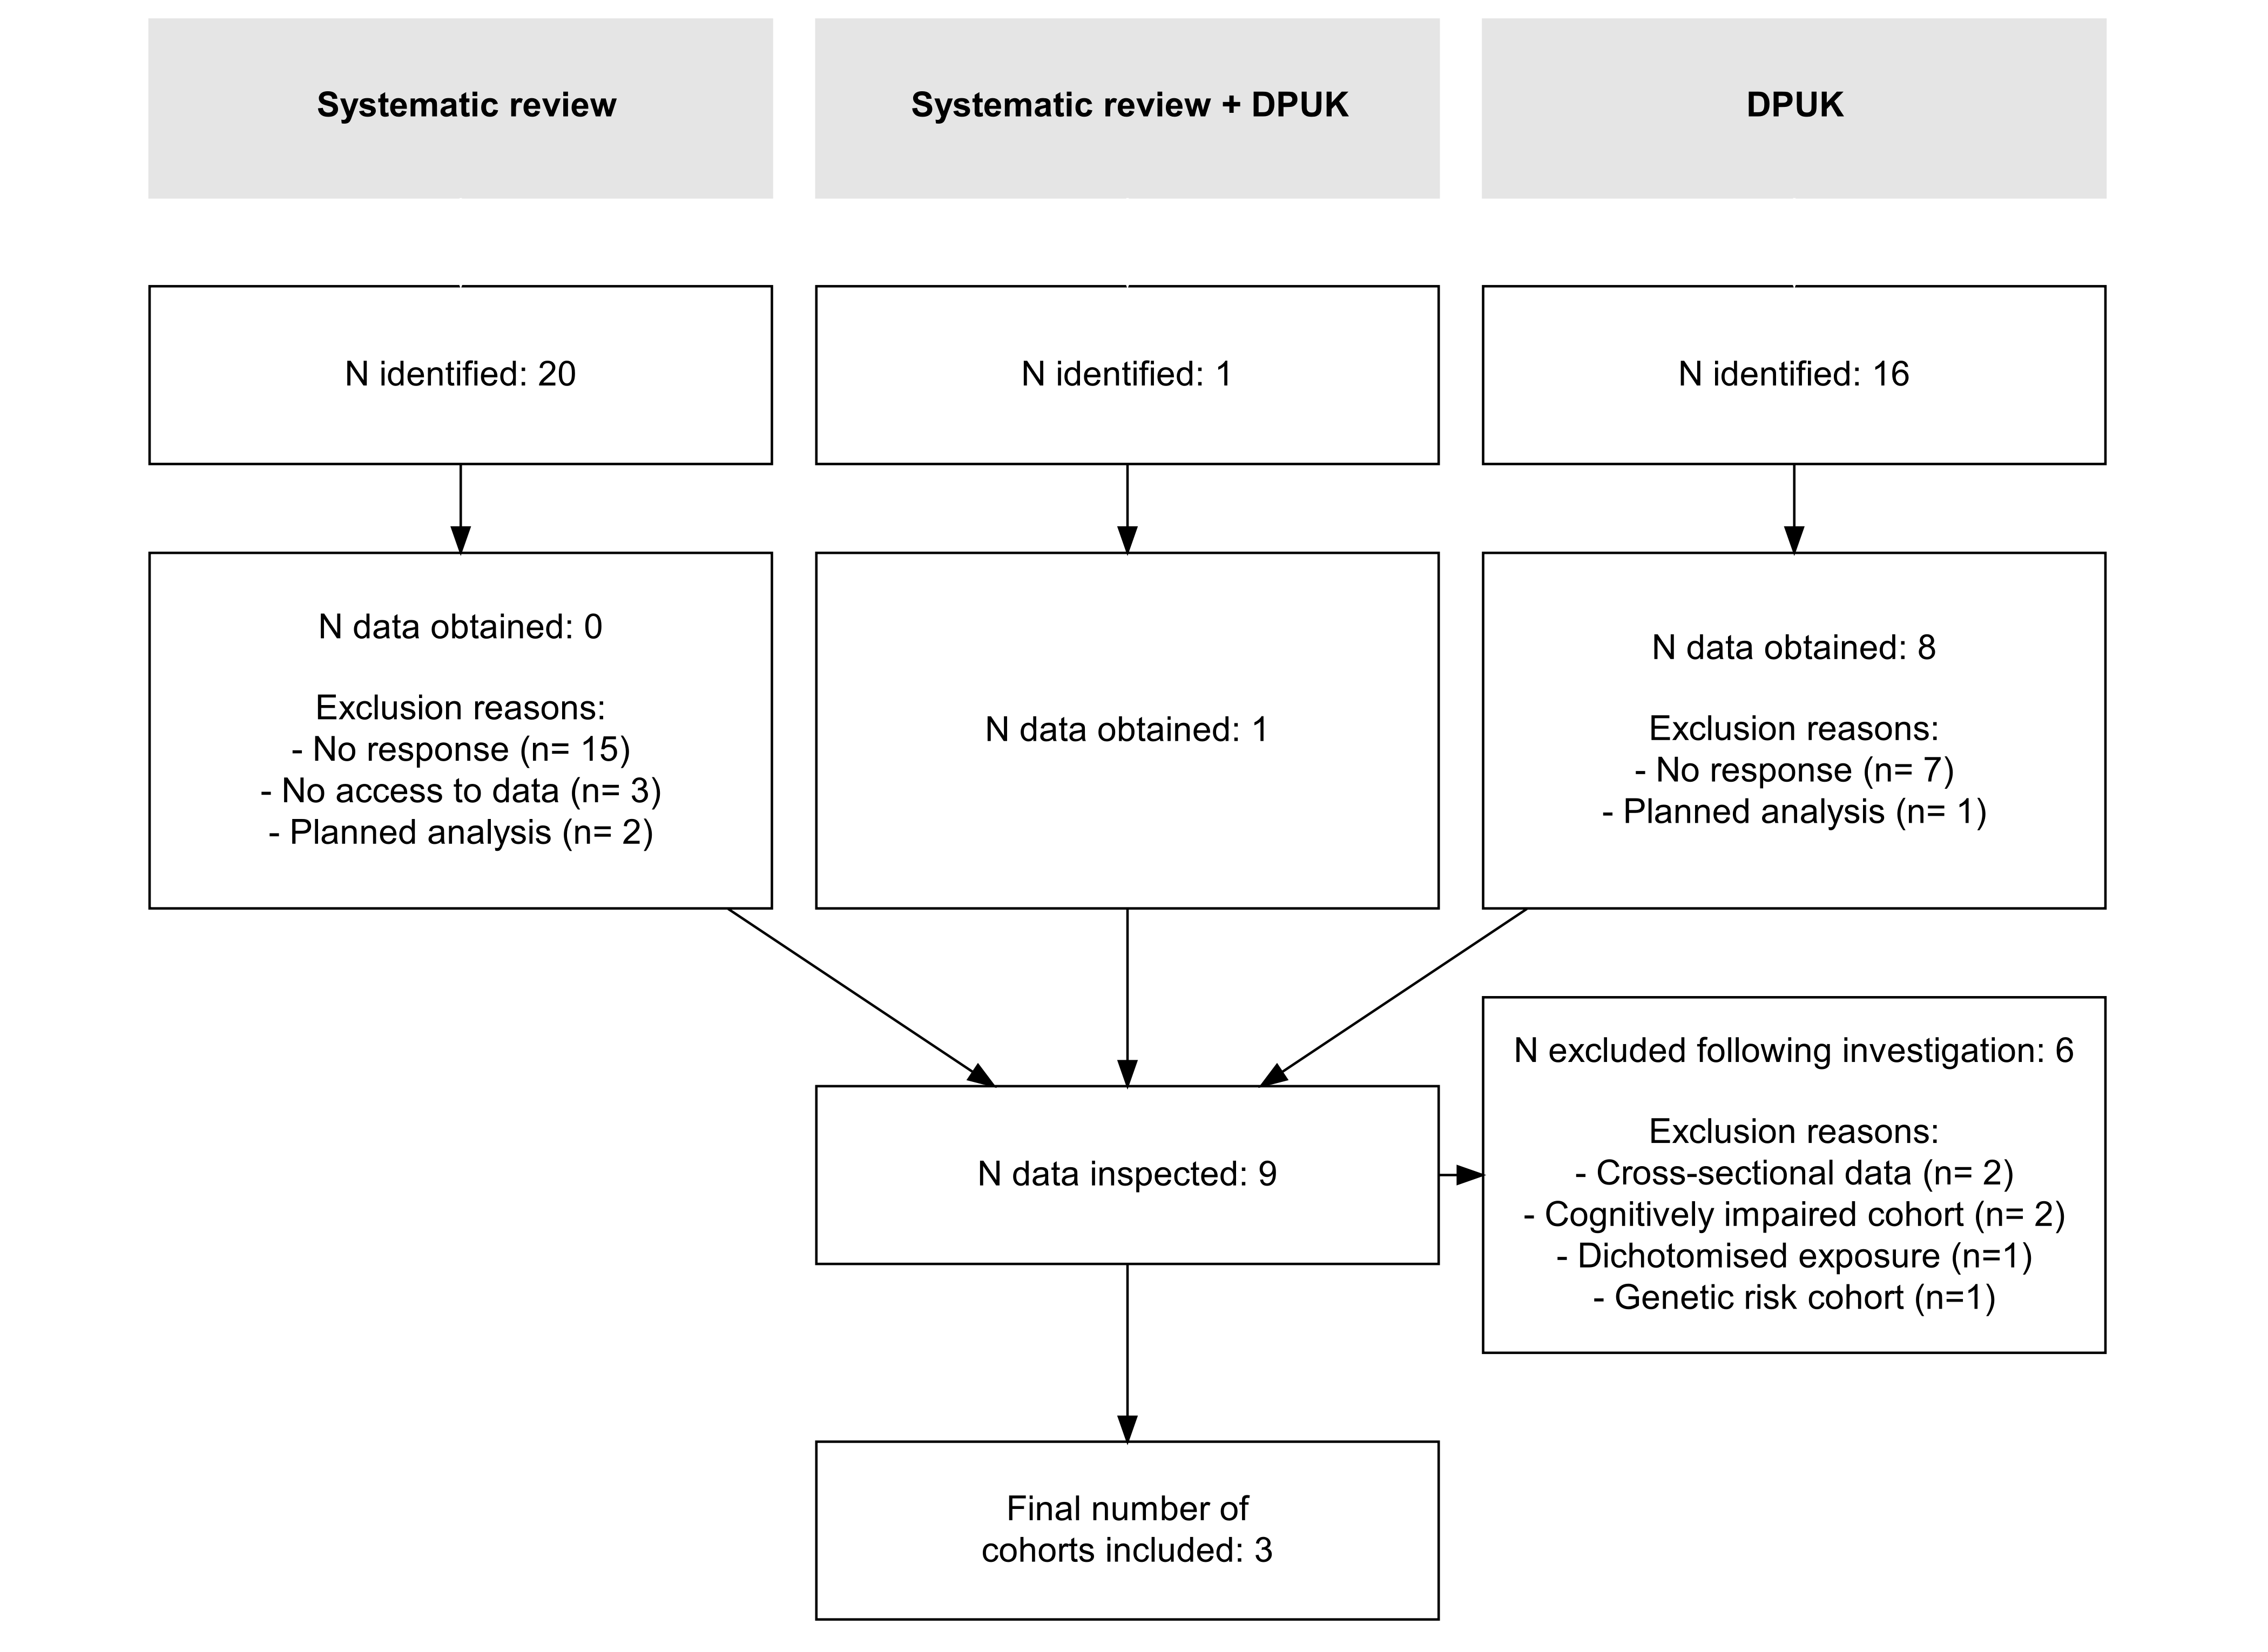
\includegraphics[width=1\linewidth]{figures/ipd/cohortFlowchart} \caption[Flowchart]{Flowchart of included cohorts, stratified by identification method (systematic review vs DPUK).}\label{fig:cohortFlowchart}
\end{figure}

As highlighted in Figure \ref{fig:cohortFlowchart}, there was little overlap between cohorts identified by the systematic review and those contained in the DPUK (1), indicating that the DPUK is a useful source of unanalysed data with respect to this question.

As highlighted in Figure \ref{fig:cohortFlowchart}, nice cohorts (8 DPUK only, 1 Systematic review + DPUK) responding positively to requests for data access. However, on inspection of data provided, six of these cohorts were excluded for a range of reasons. The exclusion reason for each cohort for which data were provided is illustrated in Table \ref{tab:dataExcluded-table}. In summary, two cohorts contained were memory-complaint cohorts, containing patients unlikely to be free of dementia at baseline (BRACE, MEMENTO). Two cohorts, despite being designed as multi-wave studies, only shared data related to a single wave and so represented cross-sectional data (Generation Scotland, NICOLA). Finally TRACK HD is a genetic cohort where cohort owners advised me that dementia will inevitably develop in mid-life driven by the Huntington's (HTT gene) mutation and that this effect would likely far outweigh the effect of lipids. Finally, the ELSA study was excluded based on the dichotomous definition of the exposure variable

~\\




\begin{table}[H]

\caption[Exclusion reasons for cohorts providing data]{\label{tab:dataExcluded-table}Exclusion reasons for cohorts providing data}
\centering
\begin{tabular}[t]{>{\raggedright\arraybackslash}p{12em}>{\raggedright\arraybackslash}p{20em}}
\toprule
\textbf{Cohort} & \textbf{Reason}\\
\midrule
BRACE & Memory complaint cohort - unlikely to be dementia free at baseline\\
\midrule
ELSA & Lipid exposure reported as a binary variable\\
\midrule
Generation Scotland & Cross-sectional - only one wave of data available\\
\midrule
MEMENTO & Memory complaint cohort - unlikely to be dementia free at baseline\\
\midrule
NICOLA & Cross-sectional - only one wave of data available\\
\midrule
\addlinespace
TRACK HD & HTT gene carriers (i.e. premanifest Huntington's Disease)\\
\bottomrule
\end{tabular}
\end{table}

~

\hypertarget{included-data-sources}{%
\subsection{Included data sources}\label{included-data-sources}}

The three data sources used in this analysis are described in detail in the following sections. Of note, all included data sources were based in the United Kingdom. This is due to the majority of included datasets being identified via the Dementia Platform UK route (Figure \ref{fig:cohortFlowchart}), which as implied by the name, has a narrow geographical focus.\textsuperscript{\protect\hyperlink{ref-bauermeister2020}{111}}

~

\hypertarget{caerphilly-prospective-study}{%
\subsubsection{Caerphilly Prospective Study}\label{caerphilly-prospective-study}}

The Caerphilly Prospective Study (CaPS) is a longitudinal study of men in South Wales, UK.\textsuperscript{\protect\hyperlink{ref-zotero-15398}{329},\protect\hyperlink{ref-elwood2013}{330}} Blood lipids (TC, LDL-c, HDL-c and TG) were measured at baseline in 1979-1983, and from Phase III (1989-1993) onwards, a battery of cognitive tests were introduced. The cohort contains data on dementia outcomes sub-classified as vascular and non-vascular dementia. Data were available for all covariates of interest except for education, BMI and ApoE4 status.

~

\hypertarget{epic-norfolk}{%
\subsubsection{Epic Norfolk}\label{epic-norfolk}}

The European Prospective Investigation of Cancer (EPIC) - Norfolk is a population-based cohort, containing men and women recruited from 35 general practices in Norfolk between 1993 and 1998.\textsuperscript{\protect\hyperlink{ref-riboli1997}{331},\protect\hyperlink{ref-riboli2002}{332}} The added evidential value of the EPIC cohort is small, given the the fact that the data obtained contains only 8 dementia events. The cohort contains no information on dementia subtype, while all covariates of interest bar ApoE4 were available.

~

\hypertarget{whitehall-ii}{%
\subsubsection{Whitehall II}\label{whitehall-ii}}

The Whitehall II study is a prospective cohort study of men and women recruited between 1985 and 1989 from the civil service in London.\textsuperscript{\protect\hyperlink{ref-marmot2005}{333}} The cohort is linked with the Hospital Episode Statistics (HES) database, a database containing details of patient events at NHS hospitals in England, which was used to define covariates at baseline and dementia outcomes.\textsuperscript{\protect\hyperlink{ref-zotero-15403}{334}} Information was available on dementia type, which was classified as all-cause dementia, Alzheimer's disease or vascular dementia. This data source contained details on all covariates of interest except for ApoE4 status.

Of note, the Whitehall II cohort was analysed in one of the included studies identified by the systematic review presented in Chapter \ref{sys-rev-heading},\textsuperscript{\protect\hyperlink{ref-tynkkynen2018}{242}} meaning that a comparison between the published result and the analysis reported here was was possible.

~

\hypertarget{ipd-covar-definition}{%
\subsection{Covariate definition \& missing data}\label{ipd-covar-definition}}

Based on available data across cohorts, smoking was classified as never/ever/current, while alcohol consumption was classified as never/ever. Education was categorised into 4 levels (None,O-levels,A-levels,Degree). BMI was treated as a continuous variable while presence of vascular co-morbidities was treated as dichotomous.

A key consideration in the definition of covariates across cohorts was the classification of age. The Whitehall II study, the largest cohort to which I had access, only shared age data in five-year age band (e.g.~40-44, 45-49, etc.). To ensure comparability across the cohorts, I created identical categories in the CaPS and EPIC data. This grouped age variable was then used in all subsequent analyses.

Missing values in collected variables was common across the cohorts. A matrix of covariates, and whether they were not available or contained missing values for each included cohort, can be seen Appendix \ref{hold}. The Whitehall II and EPIC cohorts containted data on all but one covariates of interest, while two systematically missing covariates were identified in the CaPS cohort, namely education and BMI. No included cohort provided information on the ApoE4 status of participants, and so this variable could not be adjusted for in the analysis.

~

\hypertarget{analytical-results}{%
\subsection{Analytical results}\label{analytical-results}}

\hypertarget{descriptive-statistics}{%
\subsubsection{Descriptive statistics}\label{descriptive-statistics}}

Across the three cohorts, 11,835 patients were included in this analysis (Whitehall II = 8208, EPIC = 1115, CaPS = 2512). All cohorts contained data on the four exposure variables of interest (or sufficient data from which to calculate them) and on all-cause dementia outcomes. The only other dementia outcome examined across cohorts was vascular dementia, which was reported in the CaPS and Whitehall II studies. The definitions of dementia outcomes used across cohorts can be seen in Appendix \ref{hold}. Cumulatively, there were 542 cases of all-cause dementia, with 114 further classified as vascular dementia. Summary statistics for each cohort are provided in Table \ref{tab:cohortSummary-table}.

~





\begin{table}[H]

\caption[Summary of characteristics of IPD cohorts]{\label{tab:covariateSummary-table}Summary of characteristics for cohorts included in the IPD analysis}
\centering
\begin{tabular}[t]{>{}lccc}
\toprule
\textbf{ } & \textbf{Whitehall II} & \textbf{Epic} & \textbf{CaPS}\\
\midrule
N & 8208 & 1115 & 2512\\
\midrule
Age group, Median & 45-49 & 50-54 & 50-54\\
\midrule
Male, N (\%) & 5679 (69.2) & 495 (44)\% & 2512 (100)\\
\midrule
BMI, Mean (SD) & 25.3 (3.75) & 25.8 (3.58 & -\\
\midrule
Education >18 yrs, N (\%) & 2576 (31.4) & 252 (22.6) & -\\
\midrule
\addlinespace
Smoke ever, N (\%) & 2678 (32) & 490 (43) & 2110\\
\midrule
Alcohol ever, N (\%) & 6612 (80.6) & 37 (3.3) & 2235 (89)\\
\midrule
TC, Mean (SD) & 6.49 (1.16) & 5.93 (1.08) & 5.93 (1.15)\\
\midrule
LDL-c, Mean (SD) & 4.40 (1.04) & 3.77 (0.96) & 3.74 (1.12)\\
\midrule
HDL-c, Mean (SD) & 1.43 (0.414) & 1.43 (0.41) & 1.37 (0.41)\\
\midrule
\addlinespace
TG, Mean (SD) & 1.49 (1.14) & 1.67 (1.04) & 1.83 (1.21)\\
\midrule
Dementia, N (\%) & 287 (3.5) & 8 (0.7) & 247 (9.8)\\
\midrule
Vascular dementia, N (\%) & 37 (0.5) & - & 77 (3.1)\\
\bottomrule
\end{tabular}
\end{table}

~

\hypertarget{main-effects}{%
\subsubsection{Main effects}\label{main-effects}}

The results from the main effect analysis across the varying lipid fractions on each dementia, considered can be seen in Figures \ref{fig:mainEffectDem} \& \ref{fig:mainEffectVad}, respectively. There was very weak evidence for an association of any lipid level with either all-cause or vascular dementia, with the exception of a harmful association between raised triglycerides and vascular dementia (OR: 1.40, 95\%CI: 1.19-1.63).





\begin{figure}[H]
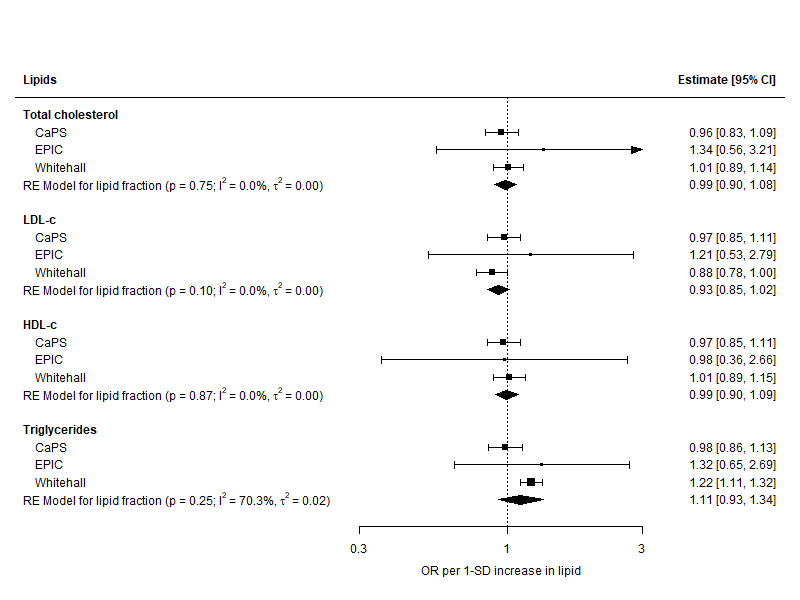
\includegraphics[width=1\linewidth]{figures/ipd/main_Dementia} \caption[IPD meta-analysis of all-cause dementia, stratified by lipid fraction]{IPD meta-analysis (model 1) of all-cause dementia outcomes, stratified by lipid fraction}\label{fig:mainEffectDem}
\end{figure}





\begin{figure}[H]
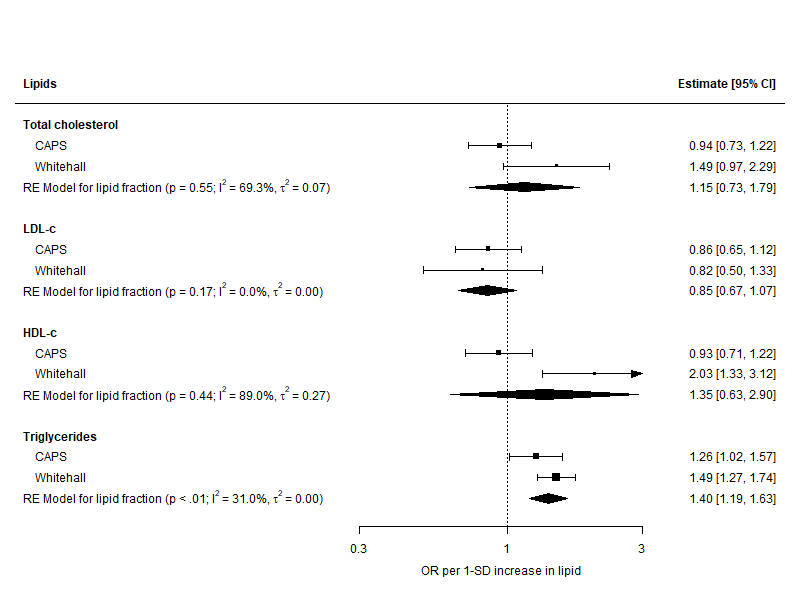
\includegraphics[width=1\linewidth]{figures/ipd/main_vasdem} \caption[IPD meta-analysis of all-cause dementia, stratified by lipid fraction]{IPD meta-analysis (model 1) of vascular dementia outcomes, stratified by lipid fraction. Note that the vascular dementia outcome was only available in the CaPS and Whitehall II cohorts.}\label{fig:mainEffectVad}
\end{figure}

Estimates from the common-set-adjusted model (Model 1: adjusted for age, sex, smoking, alcohol, presence of vascular comorbidites) were comparable to the fully-adjusted model (Model 2: Model 1 further adjusted for education and BMI) for the effect of lipids on all-cause dementia in cohorts reporting all covariates of interest (Figure \ref{fig:ipdModelComparison}).





\begin{figure}[H]
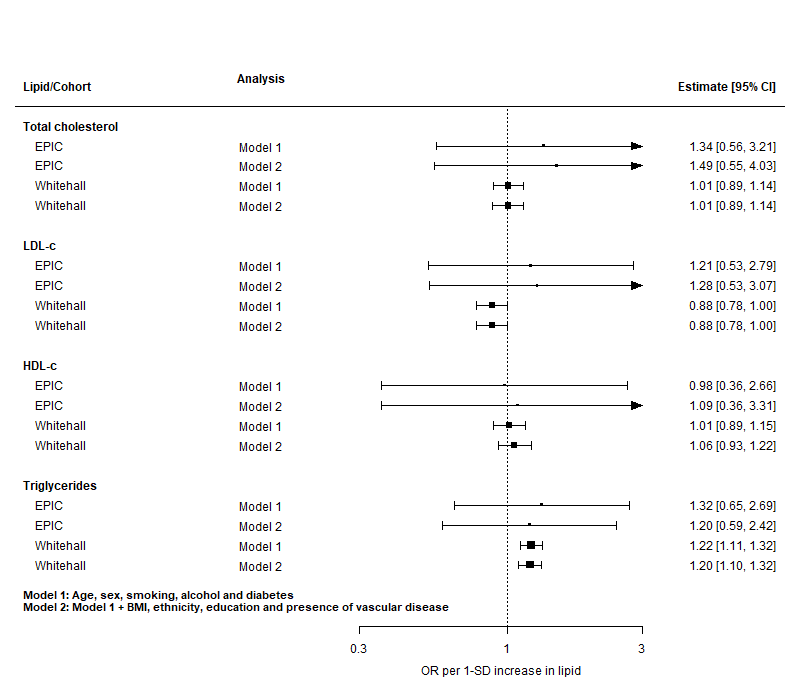
\includegraphics[width=1\linewidth]{figures/ipd/main_model_comparison} \caption[Comparison of partially and maximally adjusted results]{Comparison of results from the common-set-adjusted (Model 1) and fully-adjusted (Model 2) analyses.}\label{fig:ipdModelComparison}
\end{figure}

~

\hypertarget{interaction-effects}{%
\subsubsection{Interaction effects}\label{interaction-effects}}

For all-cause dementia, there was no evidence of an interaction of lipid levels with either age group or sex (Figures \ref{fig:interactionDementiaAge} \& \ref{fig:interactionDementiaSex}). Note that for the sex interaction analysis, the CaPS cohort was excluded as it contains only a single sex and therefore provides no information on exposure-sex interaction.





\begin{figure}[H]
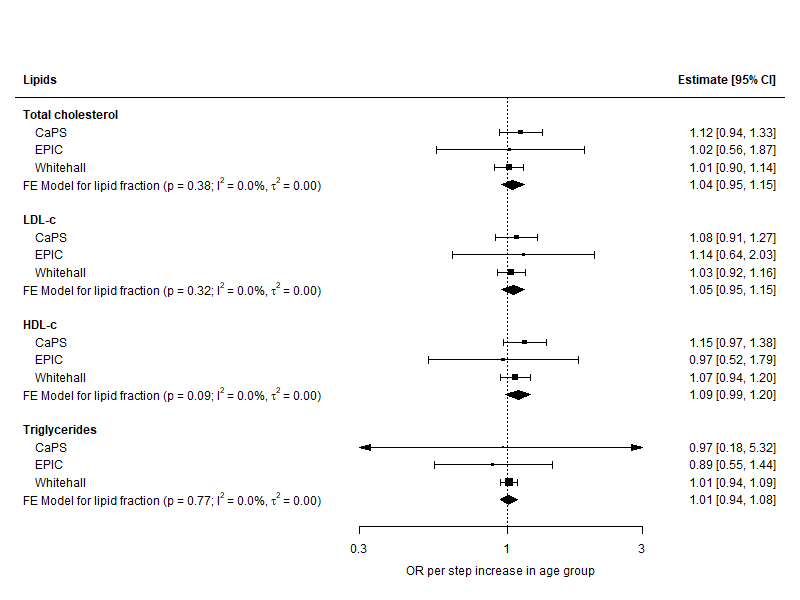
\includegraphics[width=1\linewidth]{figures/ipd/interaction_age_dementia} \caption[shortcap]{Meta-analysis of interaction terms representing the effect of a one-step increase in age group on the lipid/all-cause dementia association}\label{fig:interactionDementiaAge}
\end{figure}





\begin{figure}[H]
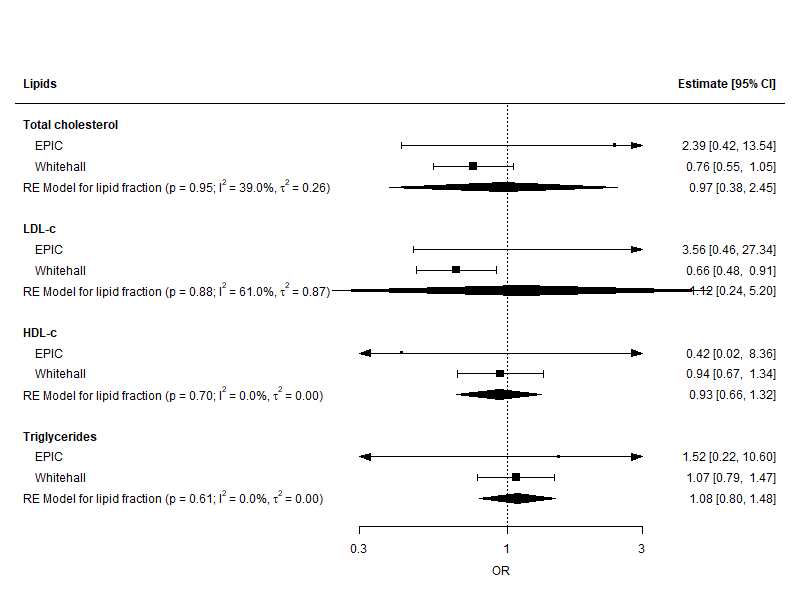
\includegraphics[width=1\linewidth]{figures/ipd/interaction_sex_dementia} \caption[shortcap]{Meta-analysis of interaction terms representing the effect of male gender on the lipid/all-cause dementia association}\label{fig:interactionDementiaSex}
\end{figure}

For the consideration of vascular dementia, I was only able to explore the effect of age, as only the CaPS and Whitehall cohorts contained details on vascular dementia as an outcome. As discussed above, the CaPS data contained a single sex excluding it from a exposure-sex analysis, leaving Whitehall II as the sole eligible study.





\begin{figure}[H]
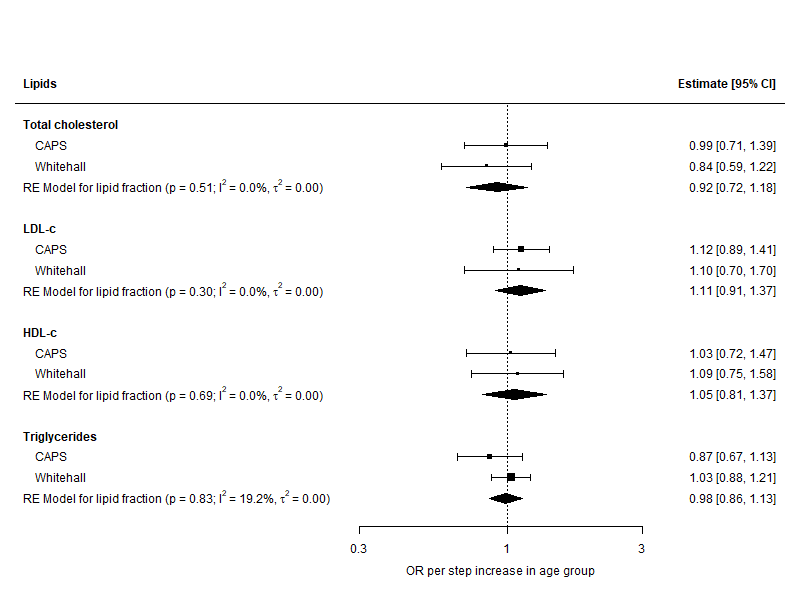
\includegraphics[width=1\linewidth]{figures/ipd/interaction_age_vasdem} \caption[shortcap]{Meta-analysis of interaction terms representing the effect of a one-step increase in age group on the lipid/vascular dementia association}\label{fig:interactionVascularAge}
\end{figure}

~

\hypertarget{comparison-with-previous-analyses}{%
\subsubsection{Comparison with previous analyses}\label{comparison-with-previous-analyses}}

For the single cohort where a previously published analysis was available (Whitehall II), results from the maximally-adjusted model for both all-cause dementia and Alzheimer's disease were comparable, with the exception of the trigluceride fraction (Figure \ref{fig:whitehallComparison}). Tynkkynen \emph{et al.}\textsuperscript{\protect\hyperlink{ref-tynkkynen2018}{242}} found a protective effect of triglycerides on all-cause dementia (HR: 0.69, 95\%CI: 0.56-0.85) while this analysis found evidence for a harmful effect (OR: 1.26, 95\%CI: 1.12-1.41).





\begin{figure}[H]
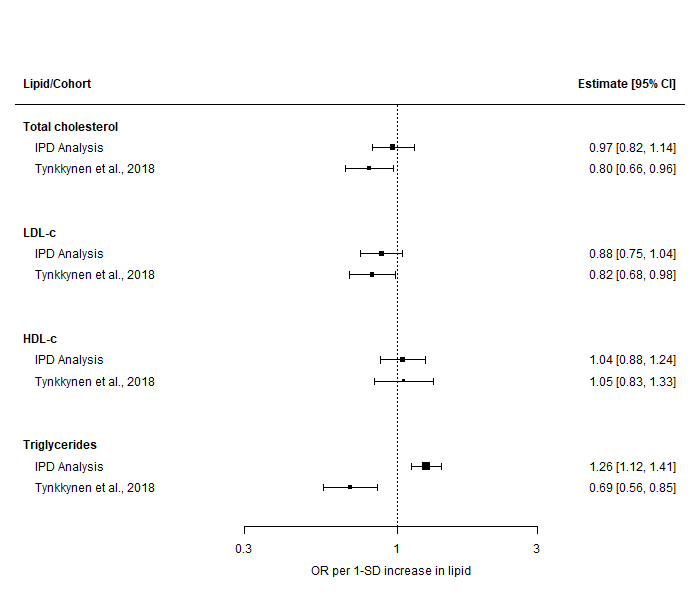
\includegraphics[width=1\linewidth]{figures/ipd/whitehall_comparison} \caption[Comparison of results across the two analysis of the Whitehall II cohort]{Comparison of results across the two analysis of the Whitehall II cohort}\label{fig:whitehallComparison}
\end{figure}

~

\hypertarget{discussion-3}{%
\section{Discussion}\label{discussion-3}}

\hypertarget{summary-of-findings-2}{%
\subsection{Summary of findings}\label{summary-of-findings-2}}

This analysis requested data from 37 data sources, but only obtained data from three, all of which were based in the United Kingdom. No evidence for an effect of lipids on the risk of dementia or related outcomes was identified, except for a harmful association of raised triglycerides with risk of vascular dementia Similarly, there was very weak evidence for an interaction of the effect of lipids levels on dementia outcomes with participants age, grouped into 5 year bands, or sex.

Similar to the analysis of CPRD data presented in the previous chapter, this discussion will not provide a detailed comparison of the results of this analysis with other published literature, except where needed to illustrate a methodological point. For a detailed comparison of the findings presented above with the existing evidence base identified by the systematic review (Chapter \ref{sys-rev-heading}), see Chapter \ref{tri-heading}.

~

\hypertarget{limitations-1}{%
\subsection{Limitations}\label{limitations-1}}

\hypertarget{low-response-rate-to-request-for-data}{%
\subsubsection{Low response rate to request for data}\label{low-response-rate-to-request-for-data}}

The obvious key limitation of this analysis is the very low response rate to requests for data access, which may bias the results if there are systematic differences between cohorts that share data and those that do not.\textsuperscript{\protect\hyperlink{ref-ahmed2012}{335}} Whether or not to press ahead with an IPD analysis in the absence of all (or even most) data is a personal decision, and some previous analyses have highlighted where they decided not to pursue an IPD study.\textsuperscript{\protect\hyperlink{ref-jaspers2014}{336}} For the purposes of this thesis, the decision was made to conduct the IPD analysis, as it provided training in pplication of the methods in addition to providing additional evidence sources that could be incorporated into the triangulation exercise detailed in Chapter \ref{tri-heading}.

A low response rate is not unexpected, given that a review of IPD studies published between 1987 and 2015 found that fewer than half managed to obtained data from greater than 80\% of studies, and that in many cases, the exact percentage of studies for which data were obtained was not accurately reported.\textsuperscript{\protect\hyperlink{ref-nevitt2017}{104}} However, it is assumed that a \textasciitilde10\% response rate is at the lower end of the scale.

There are likely several likely reasons for this low response rate to requests for data access. In general terms, there are a several well-documented reasons why data are not made readily available, including concerns regarding participant privacy and ``scooping'' or ``parasitic'' behaviour, and a lack of trust between primary and secondary researchers.\textsuperscript{\protect\hyperlink{ref-vanpanhuis2014}{109}} More specific to this analysis, individual participant data meta-analysis including studies other than randomised controlled trials have less success in obtaining individual participant data from studies.\textsuperscript{\protect\hyperlink{ref-nevitt2017}{104}} Additionally, while no evidence is available on whether the characteristics of the researcher requesting data access influences the response rate and eventual decision, there is the possibility that my position as a PhD student meant I was less likely to elicit the response rate than a well-known senior academic might. The timing of the requests for data access, coinciding with a global pandemic, may also have affected the response rate as researchers prioritised other COVID-related work.

Finally, the method of contact used (email) has been shown to be less successful in eliciting responses from authors when compared with telephoning.\textsuperscript{\protect\hyperlink{ref-danko2019}{337}} One of the reasons for this may be that the email addresses reported on publications are more likely to be out of date for older publications. Anecdotally, post-hoc investigation of a subset of cohorts revealed that several corresponding/first authors were no longer at the same institution as when the study was reported, and as a result, were unlikely to have access to the institutional email address listed on the study publication.

The barriers to data access described above are in theory what the DPUK was built to address. However, even with the help of the streamlined application process afforded by the DPUK, accessing sufficient data was a challenge. The response rate among DPUK cohorts a year after application was just 50\%. In addition, some cohorts responded that that the proposed study question was already under investigation by another group, and that they would not share the data on this basis. In light of this, a centralised database of ongoing analysis being performed in DPUK would be of enormous help. Finally, the DPUK process would be aided by a clearer distinction between those cohorts that are ``DPUK native'' (i.e.~where a copy of the data is already held on DPUK servers) versus externally hosted, as the response time for externally hosted cohorts is likely to be much longer.

~

\hypertarget{uncontrolled-confounding}{%
\subsubsection{Uncontrolled confounding}\label{uncontrolled-confounding}}

A key limitation of this analysis is the potential for uncontrolled confounding. Across all cohorts, adjustment for ApoE4 was not possible as I did not have access to genetic data on participants. As discussed above in relation to the Tynkkynen \emph{et al.} analysis, ApoE4 is a strong risk factor for both increased LDL-c levels and Alzheimer's disease.\textsuperscript{\protect\hyperlink{ref-bennet2007}{319},\protect\hyperlink{ref-safieh2019}{338}} Failing to adjust for this factor means confounding in the LDL-c fraction results is likely.

More generally, systematically missing variables meant that a trade-off between inclusion of cohort data and appropriate control for confounding was required, resulting in the potential for uncontrolled confounding due to education and BMI. However, sensitivity analysis comparing the commom-set-adjusted (Model 1) and fully-adjusted (Model 2) models in cohorts with a full complement of covariates indicated that further adjustment for BMI and education had minimal impact on the effect estimates.

\hypertarget{discrepancy-with-previous-analysis}{%
\subsubsection{Discrepancy with previous analysis}\label{discrepancy-with-previous-analysis}}

I found a qualitative difference between the association of triglycerides and all-cause dementia identified in this analysis and that previously reported by Tynkkynen \emph{et al.}\textsuperscript{\protect\hyperlink{ref-tynkkynen2018}{242}}
Investigation of this discrepancy indicated that it was likely to be due to the Whitehall snapshot that each analysis had access to, as comparison of summary statistics indicated that this analysis had substantially more dementia events (n=287 in this analysis vs.~n=114 in Tynkkynen \emph{et al.}). The covariates adjusted for in each analysis were similar, though the previous analysis had access to genetic data, allowing it to adjust for ApoE4 status. However, given that ApoE4 is a risk factor for increased LDL-c rather than triglycerides,\textsuperscript{\protect\hyperlink{ref-bennet2007}{319}} it seems unlikely that additional adjustment for this variable is responsible for the discrepancy in findings observed.

~

\hypertarget{strengths-1}{%
\subsection{Strengths}\label{strengths-1}}

\textbf{{[}Note: I feel quite negatively about this analysis, so suggestions for other strengths to flesh out this section would be welcome!{]}}

While this analysis did not manage to systematically obtain and analyse a large proportion of identified data, it did enable an analysis of two previously unanalysed datasets - the CaPS and EPIC Norfolk cohorts - providing additional data that is incorporated into the triangulation exercise reported in Chapter \ref{tri-heading}.

Additionally, it provides new evidence on a previously unexplored outcome, vascular dementia, in the Whitehall II dataset, adding to the extremely small evidence base for this outcome identified by the systematic review presented in Chapters \ref{sys-rev-method-heading} \& \ref{sys-rev-results-heading}.

~

\hypertarget{reflections-on-the-process}{%
\subsection{Reflections on the process}\label{reflections-on-the-process}}

In hindsight, attempting to undertake a large-scale IPD meta-analysis as part of a larger PhD project may have been overly ambitious. Data harmonization between cohorts in an IPD analysis is an often under-appreciated challenge,\textsuperscript{\protect\hyperlink{ref-levis2021}{324}} and in line with this, data cleaning for this analysis took substantially longer than expected. While the cohort response rate was substantially lower that expected, given the time and resource of data cleaning and harmonisation for just three cohorts, a situation in which all 37 cohorts responded positively would have been logistically challenging within the scope of my PhD.

~

\hypertarget{future-work}{%
\subsection{Future work}\label{future-work}}

While it is tempting to suggest that an IPD analysis of lipid levels be reattempted, without empirically guided approaches to increase the response rate, this may just result in a similarly small set of studies as described here. In line with the limitations considered earlier in this chapter, future methodological work could formally consider the effect of requester characteristics (sex, location, career stage) on response rates in IPD analyses.

Additionally, the production of detailed guidance for handling cases where covariates are systematically missing. Much of the literature around IPD analysis is focused on the synthesis of trials, where additional covariate information is needed primarily for the assessment of treatment-covariate interactions rather than the adjustment of the effect estimate for confounding. Given the wide availability of non-randomised cohorts, improved guidance on this challenge would support future work.

Finally, a movement towards increased use of unique persistent identification of researchers, through schemes such as the ORCID programme,\textsuperscript{\protect\hyperlink{ref-nature2009}{339}} would help with contact issues. Researchers move institutions regularly as their contracts come to an end, and so the institutional contact details provided on publications are frequently out of date.

~

\hypertarget{summary-5}{%
\section{Summary}\label{summary-5}}

\begin{itemize}
\item
  In this chapter, I performed an IPD meta-analysis to investigate the effect of blood lipid levels on risk of incident dementia. There was a very low response rate to requests for data access, resulting in the inclusion of only three cohorts.
\item
  I found very weak evidence for an association of any lipid with either all-cause or vascular dementia, except for an increased risk of vascular dementia associated with raised triglycerides. Similarly, there was very weak evidence that the association of blood lipids and dementia outcomes varied by patient age or sex.
\item
  I discussed potential reasons for the low response rate, and explored other limitations of this analysis. I highlighted the contribution of this work to the wider topic via the analysis of previously unexplored cohorts (CaPS \& EPIC) and outcomes (vascular dementia). Finally, I recommended that future research formally investigate the impact of request characteristics on requests for data.
\item
  The new evidence produced by this analysis will be incorporated, along with evidence identified or produced in the previous chapters, into the triangulation analysis presented in the following chapter.
\end{itemize}

\newpage

\hypertarget{references-5}{%
\section{References}\label{references-5}}

\begin{savequote}
Next on my list of features to be specially considered I would place the
consistency of the observed association. Has it been repeatedly observed
by different persons, in different places, circumstances and times?
\qauthor{--- Sir Austin Bradford Hill, 1965\textsuperscript{\protect\hyperlink{ref-hill1965}{340}}}\end{savequote}



\hypertarget{tri-heading}{%
\chapter{Aetiological triangulation across new and existing evidence sources}\label{tri-heading}}

\minitoc 

\hypertarget{lay-summary-6}{%
\section{Lay summary}\label{lay-summary-6}}

\textbf{TBC}

~

\newpage

\newpage

\hypertarget{triangulation-overview}{%
\section{Introduction}\label{triangulation-overview}}

Aetiological triangulation, or simply triangulation, is the process of comparing and contrasting across different sources of evidence. Triangulation is broadly comparable to Bradford-Hill's criteria of ``consistency'', that is the replication of an observed relationship across several different contexts,\textsuperscript{\protect\hyperlink{ref-hill1965}{340}} where contexts are assumed to have different underlying bias structures. More formally it can be defined as:

\begin{quote}
The practice of strengthening causal inferences by integrating results from several different approaches, where each approach has different (and assumed to be largely unrelated) key sources of potential bias.\textsuperscript{\protect\hyperlink{ref-lawlor2016}{90}}
\end{quote}

This approach represents a significant step forward from the current practice of synthesising evidence from only one type of study (e.g.~randomised controlled trials (RCTs), non-randomised studies of exposures (NRSE) or interventions (NRSI)). The most common implementation of this method to date has been in the form of \emph{qualitative triangulation} - that is the identification and narrative comparison of diverse evidence sources with respect to their underlying bias structures.\textsuperscript{\protect\hyperlink{ref-lawlor2016}{90}}

However, qualitative triangulation faces issues at scale. There is a need to include all evidence to avoid potential confirmation bias,\textsuperscript{\protect\hyperlink{ref-dubroff2018}{341}} yet as the number of evidence sources increases, it is not possible to narratively compare and contrast across multiple results in any meaningful way. This fact is illustrated by previous exemplars of triangulation only considering a small number of individual results.\textsuperscript{\protect\hyperlink{ref-lawlor2016}{90},\protect\hyperlink{ref-ference2014}{342}} To overcome this limitation, some attempts have considered the output of a meta-analysis of similarly-designed studies to be a single source of evidence, and have assessed bias in relation to this summary result. While this approach keeps the number of individual sources of evidence manageable, it loses useful information on the specific biases inherent to each result contributing to the summary estimate. For example, while it may be true that all non-randomised studies share some minimal level of bias, competing extents and directions of bias in individual results may be masked by the use of summary estimates. In addition, previous attempts at qualitative triangulation have not systematically assessed the indirectness of the results, that is the differences between the question of interest and the question addressed by a study.

Taken together, these limitations to qualitative triangulation detail a need for a more systematic way to integrate across multiple evidence sources as the number of individual results contributing to the exercise increases. One such approach is \emph{quantitative triangulation}, where results from different evidence sources are combined numerically while accounting for the key sources of bias and indirectness in each. This chapter, in addition to providing a narrative comparison of the existing and new evidence identified by this thesis, builds on recent developments in risk-of-bias assessment and methods for bias-/indirectness-adjusted meta-analysis to propose a generalised framework for quantitative triangulation. The framework, along with the methodological challenges to its implementation, is illustrated via two case studies examining the causal effect of lipids on dementia outcomes.

~

\newpage

\hypertarget{methods-3}{%
\section{Methods}\label{methods-3}}

\hypertarget{tri-data-sources}{%
\subsection{Data sources}\label{tri-data-sources}}

This triangulation exercise draws on the research produced in each of the preceding chapters. More specifically, this chapter builds on the comprehensive systematic review of existing evidence presented in Chapters \ref{sys-rev-methods-heading} \& \ref{sys-rev-results-heading}. This evidence base is then supplemented by new evidence on the association of statin use with dementia outcomes in the CPRD (Chapter \ref{cprd-analysis-heading}) and the association of lipids with dementia outcomes in previously unanalysed datasets accessed via the DPUK (Chapter \ref{ipd-heading}).

Table \ref{tab:thesisOverview-table} summarises the research each data source has attempted to address, the exposures and outcomes considered in each case, and the contribution of each chapter to the triangulation exercise presented here.

\blandscape





\begin{table}[H]

\caption[Summary of research designs included in this thesis]{\label{tab:thesisOverview-table}Summary of studies included in this thesis and used as evidence sources in this triangulation exercise. Note, Chapter \ref{sys-rev-tools-heading} is intentionally not included in this table, as it describes a research tool rather than a research study.}
\centering
\begin{tabular}[t]{>{\raggedright\arraybackslash}p{6em}>{\raggedright\arraybackslash}p{16em}>{\raggedright\arraybackslash}p{7em}>{\raggedright\arraybackslash}p{7em}>{\raggedright\arraybackslash}p{16em}}
\toprule
\textbf{Chapter} & \textbf{Research Question} & \textbf{Exposure/ Intervention} & \textbf{Outcome} & \textbf{Contibution to evidence synthesis framework}\\
\midrule
Chapter 3/4 & Based on the available evidence; \newline (i) are lipid fractions associated with subsequent dementia risk, stratified by subtype? \newline (ii) Are lipid regulating agents associated with subsequent dementia risk, stratified by subtype? \newline & Lipids (HDL-c, LDL-c, TC, TG), \newline \newline Lipid regulating agents (statins, ezetimibe, fibrates, etc.) & Dementia, stratified by subtype & Provides overview of existing evidence, including detailed risk-of-bias assessments for each result\\
\midrule
Chapter 5 & Are lipid regulating agents associated with dementia risk in a large scale electonic health record database? \newline & Seven classes of lipid regulating agents & Dementia, stratified by subtype & Provides additional observational data on vascular dementia (under-represented in the literature) \newline \newline Provides a source of observational evidence created using a method with distinct sources of bias to those identified by the systematic review\\
\midrule
Chapter 6 & Are lipid levels associated with dementia risk in an individual participant data meta-analysis? \newline & Lipids (HDL-c, LDL-c, TC, TG) & All-cause dementia \newline VaD & Provides additional evidence from unanalysed datasets \newline \newline Provides additional observational data on vascular dementia (under-represented in the literature)\\
\bottomrule
\end{tabular}
\end{table}

\elandscape

~

\hypertarget{qual-tri}{%
\subsection{Qualitative triangulation}\label{qual-tri}}

As discussed in the introduction to this Chapter (Section \ref{triangulation-overview}), as part of a narrative synthesis of the evidence all information sources were initially grouped by outcome, and the findings from each source were narratively compared and contrasted. Potential reasons for heterogeneity between study designs were examined with specific reference to the risk-of-bias assessments performed.

This analysis built on the detailed risk-of-bias assessments performed and presented as part of the systematic review (Chapters \ref{sys-rev-methods-heading} \& \ref{sys-rev-results-heading}). Similarly, risk-of-bias assessments were performed for each new source of evidence presented in this thesis. The risk of bias tools used to assess each result are described in detail in Section \ref{risk-of-bias}, but in summary, RCTS were assessed using the RoB 2 tool;\textsuperscript{\protect\hyperlink{ref-sterne2019}{93}} NRSI using the ROBINS-I tool;\textsuperscript{\protect\hyperlink{ref-sterne2016}{157}} NRSE using the ROBINS-E tool (see Section \ref{rob-tools-nrse});\textsuperscript{\protect\hyperlink{ref-morganr2020}{160},\protect\hyperlink{ref-french2019}{161}} and MR studies using the Mamluk et al.~tool.\textsuperscript{\protect\hyperlink{ref-mamluk2020}{163}}

~

\hypertarget{quantitative-triangulation}{%
\subsection{Quantitative triangulation}\label{quantitative-triangulation}}

In addition to a qualitative discussion of the evidence, I attempted to integrate the numerical results of the multiple approaches under a proposed quantitative triangulation framework. This approach incorporates recent advancements in the way that bias in results is assessed (namely the move to domain-based assessment tools)\textsuperscript{\protect\hyperlink{ref-sterne2019}{93}} and existing methods for bias-/indirectness-adjusted meta-analysis\textsuperscript{\protect\hyperlink{ref-turner2009}{343}} to illustrate how causal questions could be addressed under this framework.

This proposed framework involves several steps, described in detail in the following sections. In summary, these steps are:

\begin{enumerate}
\def\labelenumi{\arabic{enumi}.}
\tightlist
\item
  Define the causal question of interest
\item
  Identify of relevant evidence sources and standardise effect directions
\item
  Assess and visualise the extent and direction of bias in each result
\item
  Define modifying terms for bias and indirectness in each result
\item
  Calculate bias-/indirectness-adjusted results and perform meta-analysis
\end{enumerate}

In order to illustrate the bias-/indirectness adjustment process detailed in the subsequent sections, the process for calculating the adjusted estimate is described in detail for a single result. Following this, the framework is applied to two case studies, as defined below.

~

\hypertarget{definition-of-the-causal-questions-of-interest-case-studies}{%
\subsubsection{Definition of the causal questions of interest (case-studies)}\label{definition-of-the-causal-questions-of-interest-case-studies}}

Using the ROBINS-E framework,\textsuperscript{\protect\hyperlink{ref-morganr2020}{160}} I defined the parameters of my causal questions of interest:

\textbf{Case study \#1: Effect of mid-life LDL-c on Alzheimer's disease}

\begin{itemize}
\tightlist
\item
  \emph{Population of interest}: General population
\item
  \emph{Exposure of interest}: Low density lipoprotein cholesterol
\item
  \emph{Exposure window of interest}: Mid-life (45-60)
\item
  \emph{Summary measure of exposure over time}: Average exposure
\item
  \emph{Outcome of interest:} Alzheimer's disease
\end{itemize}

\textbf{Case study \#2: Effect of mid-life triglycerides on vascular dementia}

\begin{itemize}
\tightlist
\item
  \emph{Population of interest}: General population
\item
  \emph{Exposure of interest}: Triglycerides
\item
  \emph{Exposure window of interest}: Mid-life (45-60)
\item
  \emph{Summary measure of exposure over time}: Average exposure
\item
  \emph{Outcome of interest:} Vascular dementia
\end{itemize}

~

These questions were chosen for several reasons. Firstly, work presented in previous chapters had identified some evidence for an association in these exposure/outcome pairs. Secondly, given the long prodomal period between the onset of physiological changes in the brain and presentation of dementia symptoms, it seems likely that conditions during the mid-life period are particularly important. Finally, examining the causal impact of a lipid faction on a specific outcome (e.g.~Alzheimer's disease), rather than a composite outcome (e.g.~all-cause dementia), focuses on an single causal pathway rather than including several conditions in the outcome definition that likely have very different mechanisms of disease. In addition, previous work presented in this thesis illustrated that the component conditions (in this case Alzheimer's disease and vascular dementia) are likely to be subject to very different confounding structures (see Section \ref{hold}), and use of an composite all-cause outcome in the triangulation framework may mask this.

~

\hypertarget{identify-relevant-results}{%
\subsubsection{Identify relevant results}\label{identify-relevant-results}}

Once the causal question of interest had been defined, relevant individual results were obtained from the data sources described in Section \ref{tri-data-sources}. In a broad sense, this meant extracting results that examined the relationship between the exposure/outcome pair, either directly (e.g.~non-randomised studies of LDL-c levels) or indirectly (e.g.~non-randomised studies of statins, or Mendelian randomisation studies using genetic instruments for LDL-c levels).

Once the set of relevant results were identified, effects were standardised to refer to the risk resulting from a ``reduction'' in the lipid fraction. For both non-randomised studies and Mendelian randomisation analysis of lipid levels, the association is usually reported per 1-SD increase in the lipid fraction. In this case, the effect estimates were inverted to ensure consistency across study designs.

~

\hypertarget{assess-risk-and-direction-of-bias-in-each-result}{%
\subsubsection{Assess risk and direction of bias in each result}\label{assess-risk-and-direction-of-bias-in-each-result}}

Risk of bias was assessed for each result as discussed in Section \ref{qual-tri}. For the sake of consistency and ease of computing, I mapped the different acceptable risk-of-bias judgements in each tool to a harmonised set: ``Low'', ``Moderate'', and ``High''. The exact mapping can be seen in Table \ref{tab:robLevelsMapping-table}. Of note, no mapping was performed for the critical risk-of-bias levels present in the tools for non-randomised studies. This is because current best practice in evidence synthesis is to exclude all studies at critical risk of bias for further quantitative synthesis.\textsuperscript{\protect\hyperlink{ref-sterne2016}{157}}

~\\




\begin{table}[H]

\caption[Mapping of risk-of-bias judgements across assessment tools]{\label{tab:robLevelsMapping-table}Mapping of the different acceptable levels of bias across the assessment tools to a harmonised set. Note that no mapping for ``Critical'' risk of bias was performed, as best practice reccommends that studies at critical risk of bias are excluded from quantitative syntheses.}
\centering
\begin{tabular}[t]{>{}cccc}
\toprule
\textbf{Harmonised} & \textbf{RoB2} & \textbf{ROBINS-I / ROBINS-E} & \textbf{MR}\\
\midrule
\textbf{Low} & Low & Low & Low\\
\midrule
\textbf{Moderate} & Some concerns & Moderate & Moderate\\
\midrule
\textbf{High} & High & Serious & High\\
\midrule
\textbf{-} & - & Critical & -\\
\bottomrule
\end{tabular}
\end{table}

~

In addition to assessing the extent of bias, as defined by the three levels detailed above, I attempted to record the predicted direction and type of bias in each domain. This was achieved via an additional question at the end of each bias domain, which asked assessors to predict the expected direction of bias in that domain. Note that this question is currently only formally included in two existing tools (ROB2/ROBINS-I), but I employed an identical approach during assessment of non-randomised studies of exposure and Mendelian randomisation studies. Acceptable responses to this question included:

\begin{itemize}
\tightlist
\item
  ``Favours experimental''/``Favours comparator'' (defines an additive bias)
\item
  ``Towards null''/``Away from null'' (defines a proportional bias)
\item
  ``Unpredictable''
\end{itemize}

As indicated in the options above, the response to this question is also used to determine the predicted type of bias as either additive or proportional. Proportional biases are dependent on the magnitude of the effect, while additive biases are not.\textsuperscript{\protect\hyperlink{ref-turner2009}{343}}

For additive biases, determining the absolute direction of bias was simply a case of whether the bias is expected to shift the effect estimate to the left or right on an imaginary forest plot. For example, the estimate would be shifted to the right if a bias was predicted to favour the comparator (Figure \ref{fig:exampleDirection}).

In contrast, for proportional biases, whether the estimate should be increased or decreased proportionally depends on the current position of the point estimate relative to the null. For example, if the effect estimate represents a protective effect (below the null), then bias towards the null would be adjusted for by moving the effect estimate proportionally to the right. In contrast, if the effect of the intervention is harmful (effect estimate above the null), bias towards the null would be adjusted for by moving the effect estimate proportionally to the left. Both scenarios are illustrated using example data in Figure \ref{fig:exampleDirection}.





\begin{figure}[H]
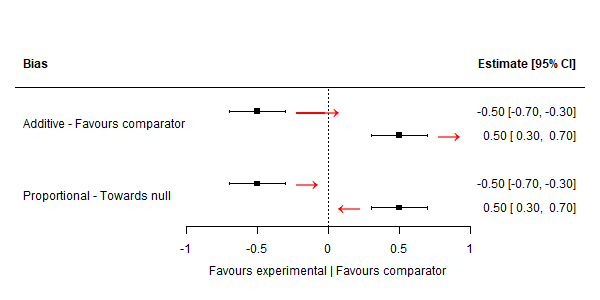
\includegraphics[width=1\linewidth]{figures/tri/exampleDirection} \caption[Illustration of calculating the absolute direction of biases, based on bias type.]{Illustration of calculating the absolute direction of biases (indicated by arrows), based on bias type. For additive biases, the direction is consistent regardless of the position of the effect estimate relative to the null - bias ``favouring the comparator'' will always pull the effect estimate to the right. In contrast, the position of the effect estimate is accounted for when determining the absolute direction of proportional biases, defined as towards or away from the null.}\label{fig:exampleDirection}
\end{figure}

The predicted direction and type of bias were not recorded for domains at ``Low'' risk of bias. Finally, for some domains, only one type of bias is allowed. For example, in the confounding domains in the ROBINS-I/ROBINS-E tools, only the ``Favours experimental''/``Favours comparator'' and ``Unpredictable'' options are available, meaning that bias in this domain will always be considered additive.

~

\hypertarget{visualisation-of-extent-and-direction-of-bias}{%
\subsubsection{Visualisation of extent and direction of bias}\label{visualisation-of-extent-and-direction-of-bias}}

To aid with the quantitative triangulation exercise, I created a new method to visualise the extent, direction and type of bias in each result, enabling detailed comparison across different studies contributing to a synthesis. Similar to the standard paired forest plots introduced in Chapter \ref{sys-rev-}, these ``bias direction'' plots show the level (or extent) of bias across the domains for each result reported using coloured blocks. However, in contrast to the previous forest plots, symbols are used to illustrate the predicted absolute direction of bias in that domain. Distinct symbol pairs are used to denote additive and proportional biases.

~

\hypertarget{assign-modifying-values-to-riskdirection-of-bias}{%
\subsubsection{Assign modifying values to risk/direction of bias}\label{assign-modifying-values-to-riskdirection-of-bias}}

Following definition of the extent, type and direction of bias in each domain, I assigned a prior distribution on the log scale to each combination. For example, a ``high'' additive bias in \(j\)th domain of the \(i\)th study is defined as \(\delta_{i,j}^{\mathrm{High}}\) and uncertainty around this estimate is given by a distribution:

\begin{equation}
  \delta_{i,j}^{\mathrm{High}} = f(\mu_{i,j}^{\mathrm{High}}, \sigma_{i,j}^{\mathrm{High}})
  \label{eq:name}
\end{equation}

The sign of \(\mu_{i,j}^{\mathrm{High}}\) is defined by the absolute direction of the bias. If the bias is expected to pull the effect to the left, \(\mu_{i,j}^{\mathrm{High}}\) is given a negative sign, and if it is expected to pull the effect to the right, it is given a positive sign.

One key feature of the domain-based risk-of-bias tools is that the domains are considered interchangeable - i.e.~a ``high'' judgement in one domain is equivalent to a ``high'' judgement in any other. As such, for this analysis, I assumed that the distributions assigned to each extent of bias were identical across all values of \(j\), that is, were identical for all domains in the risk-of-bias assessment tool. To illustrate for additive biases:

\[
\delta_{i,1}^{\mathrm{High}} = \delta_{i,2}^{\mathrm{High}} = ... = \delta_{i,j}^{\mathrm{High}}
\]

and similarly

\[
\delta_{i,1}^{\mathrm{Moderate}} = \delta_{i,2}^{\mathrm{Moderate}} = ... = \delta_{i,j}^{\mathrm{Moderate}}
\]

Reasonable values for the position and spread of the prior distributions were informed by a previously-reported expert bias elicitation exercise.\textsuperscript{\protect\hyperlink{ref-turner2009}{343}} Using open data from that study, I calculated the mean values for the mean and variance of the adjustment distributions across all biases considered by that exercise (see Appendix @ref(?) for more details on how these were calculated). For the purposes of this illustrative analysis and to highlight the generalised nature of the code used to perform the analysis (see Section \ref{tri-software}), I used the calculated values to inform two scenarios of modifying distributions (Table \ref{tab:priorsAdd-table}) for additive biases, and a single set for proportional biases. In the first scenario, the relationship between the position assigned to each additive judgement is linear. In the second scenario, the step from ``Moderate'' to ``High'' is twice that from ``Low'' to ``Moderate''. Across both additive and proportional biases, the variance of the ``High'' judgement distribution was defined to be greater than that of the ``Moderate'' judgement.

~





\begin{table}[H]

\caption[Prior distributions mapped to different extents of bias.]{\label{tab:priorsAdd-table}Prior distributions for extent and type of bias under two scenarios, on the log scale. Note that the distributions for proportional biases were kept consistent across the two scenarios.}
\centering
\begin{tabular}[t]{>{}lccc}
\toprule
\multicolumn{1}{c}{\textbf{Bias Level}} & \multicolumn{2}{c}{\textbf{Additive bias}} & \multicolumn{1}{c}{\textbf{Proportional bias}} \\
\textbf{} & \textbf{Scenario 1} & \textbf{Scenario 2} & \textbf{}\\
\midrule
\textbf{Low} & - & - & -\\
\midrule
\textbf{Moderate} & N(.08, .05) & N(.08, .05) & N(.03, .016)\\
\midrule
\textbf{High} & N(.16, .1) & N(.24, .1) & N(.06, .032)\\
\bottomrule
\end{tabular}
\end{table}

~

Where the direction of bias in a domain was unpredictable for a given result, the mean of the prior distribution for that domain was set to 0 but the appropriate variance for the recorded extent of bias was retained (e.g.~for an unpredictable ``High'' additive bias, the distribution would be \(N(0,0.1)\) under Scenario 1). In other words, adjusting for bias in a domain with an unpredictable direction of bias has no impact on the position of the effect estimate but does increase the uncertainty around it.

~

\hypertarget{assessing-and-assigning-prior-values-to-indirectness}{%
\subsubsection{Assessing and assigning prior values to indirectness}\label{assessing-and-assigning-prior-values-to-indirectness}}

The indirectness of a result (also termed external bias, external validity, relevance, generalisability, or applicability) is defined here as the discrepancy between the research question addressed by the ``idealised'' study and the causal question of interest.

An identical approach was employed to assess, and assign prior distributions to, the indirectness in each result. The target question for each result was compared against the causal question of interest with respect to three domains, defined as important by the GRADE framework for assessing the certainty of evidence:\textsuperscript{\protect\hyperlink{ref-guyatt2011}{344}} population, intervention/exposure, and outcome. I again used the scale of ``Low/''Moderate``/''High" to quantify the extent of indirectness in each domain. All indirectness was defined \emph{a priori} as being proportional in nature (i.e.~depending on the magnitude of the effect), in line with previous work on this topic.\textsuperscript{\protect\hyperlink{ref-turner2009}{343},\protect\hyperlink{ref-thompson2011}{345}} As above, data from the previous elicitation exercise were used to inform reasonable prior distributions for each level of indirectness (Table \ref{tab:priorsIndirect-table}).

~





\begin{table}[H]

\caption[Prior distributions mapped to different extents of bias.]{\label{tab:priorsIndirect-table}Prior distributions for extent and type of bias under two scenarios, on the log scale. Note that the distributions for proportional biases were kept consistent across the two scenarios.}
\centering
\begin{tabular}[t]{>{}lc}
\toprule
\textbf{Bias Level} & \textbf{Proportional bias}\\
\midrule
\textbf{Low} & -\\
\midrule
\textbf{Moderate} & N(.06, .016)\\
\midrule
\textbf{High} & N(.12, .032)\\
\bottomrule
\end{tabular}
\end{table}

~

As an illustrative example, consider the first causal question of the interest in this exercise, the effect of LDL-c in mid-life on Alzheimer's disease. Here, studies of lipids levels in this time period would require minimal adjustment, whereas studies examining statin use (indirect exposure/intervention) in late-life (indirect population) would be down-weighted due to reduced relevance to the causal question.

~

\hypertarget{combine-in-a-bias-adjusted-meta-analysis}{%
\subsubsection{Combine in a bias-adjusted meta-analysis}\label{combine-in-a-bias-adjusted-meta-analysis}}

Using the the method reported in Turner \emph{et al.},\textsuperscript{\protect\hyperlink{ref-turner2009}{343}} total additive and proportional bias and indirectness were calculated and used to define an adjusted estimate for each result included in the synthesis.

The adjusted estimate for each result, \(\hat\theta\), is defined as:

\begin{equation}
  \hat{\theta} = \frac{y_i - \mu_{i\beta}^{\mathrm{In}}\mu_{i\delta}^{\mathrm{In}} - \mu_{i\delta}^{\mathrm{B}}}{\mu_{i\beta}^{\mathrm{B}}\mu_{i\beta}^{\mathrm{In}}}
  \label{eq:adjusted-mean}
\end{equation}

where \(\mu_{i\delta}^{\mathrm{B}}\) and \(\mu_{i\beta}^{\mathrm{B}}\) refer to the total additive and proportional bias, and \(\mu_{i\delta}^{\mathrm{In}}\) and \(\mu_{i\beta}^{\mathrm{In}}\) refer to the total additive and proportional indirectness. Note that in this exercise, the total additive indirectness \(\mu_{i\beta}^{\mathrm{In}} = 1\), as all indirectness was defined \emph{a priori} as being proportional.

The standard error of this estimate is then calculated as:

\begin{equation}
  \mathrm{SE}(\hat{\theta})=\left(\frac{1}{\mu_{i \beta}^{\mathrm{B}} \mu_{i \beta}^{\mathrm{In}}}\right)^{2}\left(s_{i}^{2}+\left(\mu_{i \beta}^{\mathrm{B}} 2+\sigma_{i \beta}^{\mathrm{B}}\right)\left(\hat{\theta}^{2} \sigma_{i \beta}^{\mathrm{In} 2}+\sigma_{i \delta}^{\mathrm{In} 2}\right)+\sigma_{i \beta}^{\mathrm{B}}\left(\hat{\theta} \mu_{i \beta}^{\mathrm{In}}+\mu_{i \delta}^{\mathrm{In}}\right)^{2}+\sigma_{i \delta}^{\mathrm{B} 2}\right)
  \label{eq:adjusted-se}
\end{equation}

Once each individual result had been adjusted using this approach, I performed a random effects meta-analysis using the unadjusted and adjusted results. I also compared the adjusted results under the two scenarios of additive bias defined. results. I extracted the overall effect estimates, along with measures of heterogeneity in each case (\(\tau^2\), \(I^2\)).\textsuperscript{\protect\hyperlink{ref-higgins2003}{346},\protect\hyperlink{ref-higgins2008}{347}}

~

\hypertarget{results-3}{%
\section{Results}\label{results-3}}

\hypertarget{qualitative-triangulation-narrative-comparison}{%
\subsection{Qualitative triangulation / narrative comparison}\label{qualitative-triangulation-narrative-comparison}}

\textbf{{[}Question: the ``strength of evidence'' language here makes for fairly ambiguous reading - e.g.~``very weak evidence''. Should I also include the effect estimates from each approach, which will help to clarify, if it is a narrative synthesis?{]}}

I identified no consistent effect of any lipid fraction on any dementia outcome across the evidence sources presented in this thesis, through there was some suggestion of a protective effect of LDL-c lowering (via statin use) on all-cause dementia and Alzheimer's disease, and a harmful effect of raised triglyceride levels on vascular dementia.

~

\hypertarget{all-cause-dementia}{%
\subsubsection{All-cause dementia}\label{all-cause-dementia}}

Analysis of lipid levels across both the systematic review (Chapter \ref{hold}) and the IPD analysis (Chapter \ref{hold}) both found extremely weak evidence for an association of any lipid fraction with all-cause dementia. Similarly, both a meta-analysis of RCTs of statin use and of MR analyses of genetic instruments that mimic statin use found very weak evidence of an association, providing indirect evidence on the effect of LDL-c lowering on this outcome.

In contrast, the meta-analysis of NRSI of statin use found a slight protective effect, though many of the studies in this analysis were found to be at risk of immortal time bias, which would be expected to favour the intervention. Finally, analysis of the association of statin use with all-cause dementia in the CPRD (Chapter \ref{hold}) found evidence of a harmful effect, though this is likely to be driven by the substantial confounding by indication identified in the vascular dementia subgroup.

For fibrates, an alternative lipid-regulating agent, there was some evidence of an increased risk of all-cause dementia in the CPRD, though this did not replicate in the meta-analysis of previous studies examining the association of fibrates and all-cause dementia.

~

\hypertarget{alzheimers-disease}{%
\subsubsection{Alzheimer's disease}\label{alzheimers-disease}}

Meta-analysis of lipid levels in the systematic review (Chapter \ref{hold}) found extremely weak evidence for an association of any lipid fraction with Alzheimer's disease. Similarly, a meta-analysis of MR analyses of genetic instruments that mimic statin use found very weak evidence of an association.

In contrast, the meta-analysis of NRSI of statin use found a slight protective effect, though similar to the all-cause dementia outcome, many of the studies in this analysis were found to be at risk of immortal time bias. However, the CPRD analysis (Chapter \ref{hold}) attempted to account for this potential bias through the use of time-varying treatment indicator. It found very weak evidence for an effect, though the potential for differential misclassification on the basis of the exposure limit the validity of this finding.

The IPD analysis (Chapter\ref{hold}) provided no information on this outcome, as the sole cohort containing data on Alzheimer's disease (Whitehall II) had previously been analysed in respect to this outcome and so was included in the meta-analysis of NRSE.

~

\hypertarget{vascular-dementia}{%
\subsubsection{Vascular dementia}\label{vascular-dementia}}

There was a general absence of existing evidence on vascular dementia outcomes. Meta-analysis of the small number of studies examing lipid levels in the systematic review (Chapter \ref{hold}) found extremely weak evidence for an association of any lipid fraction with vascular dementia. Similarly, a meta-analysis of statin use found very weak evidence for an effect on this outcome. The CPRD analysis (Chapter \ref{hold}) found evidence for a harmful association of statin use with vascular dementia, though this finding is likely to be the result of severe confounding by indication, as identified through the use of control outcomes.

Finally, the IPD analysis (Chapter @Ref(hold)) provided supporting evidence for the absence of an effect of any fraction on vascular dementia, with the sole exception of triglycerides. Raised triglycerides were associated with an increased incidence of vascular dementia across two previously unanalysed cohorts though there is the potential for uncontrolled confounding due to the limited information on covariates available. With respect to evidence on treatments for hypertriglyceridemia, examination of fibrates in the CPRD provided very weak evidence of an association with vascular dementia.

~

\hypertarget{quantitative-triangulation-1}{%
\subsection{Quantitative triangulation}\label{quantitative-triangulation-1}}

\hypertarget{single-study}{%
\subsubsection{Single study}\label{single-study}}

As an illustrative example, the bias and indirectness inherent to the estimate of the effect of statin use on Alzheimer's disease in the CPRD are considered here. For this result, there were three domains at greater than low risk of bias: Bias due to confounding, Bias due to definition of the outcome, and Bias in the selection of the reported result (Figure \ref{fig:biasDirectionSingle}). In Domain 1 (bias due to confounding), the study did not adjust for ApoE4 status, which is predicted to mask any true association between statins and Alzheimer's disease (see Section \ref{cprd-limitations} for a fuller discussion). As such, the bias is predicted to \emph{favour the comparator} and so the absolute direction of bias is to the right. In Domain 7 (bias in measurement of the outcome), there was a high risk of differential misclassification on the basis of the exposure. Here, history of statin use may make a diagnosis of vascular dementia more likely than Alzheimer's disease, and so for this outcome, this bias is predicted to \emph{favour the experiment} (in this case, an intervention). As such, the absolute direction of bias is to the left. In Domain 7 (bias in selection of the reported result), for consistency with the other NRSI, in the absence of a protocol the bias is assumed to be \emph{away from the null}. Given the position of the effect estimate below the null, the absolute direction of bias in this domain is to the left.

~\\




\begin{figure}[H]
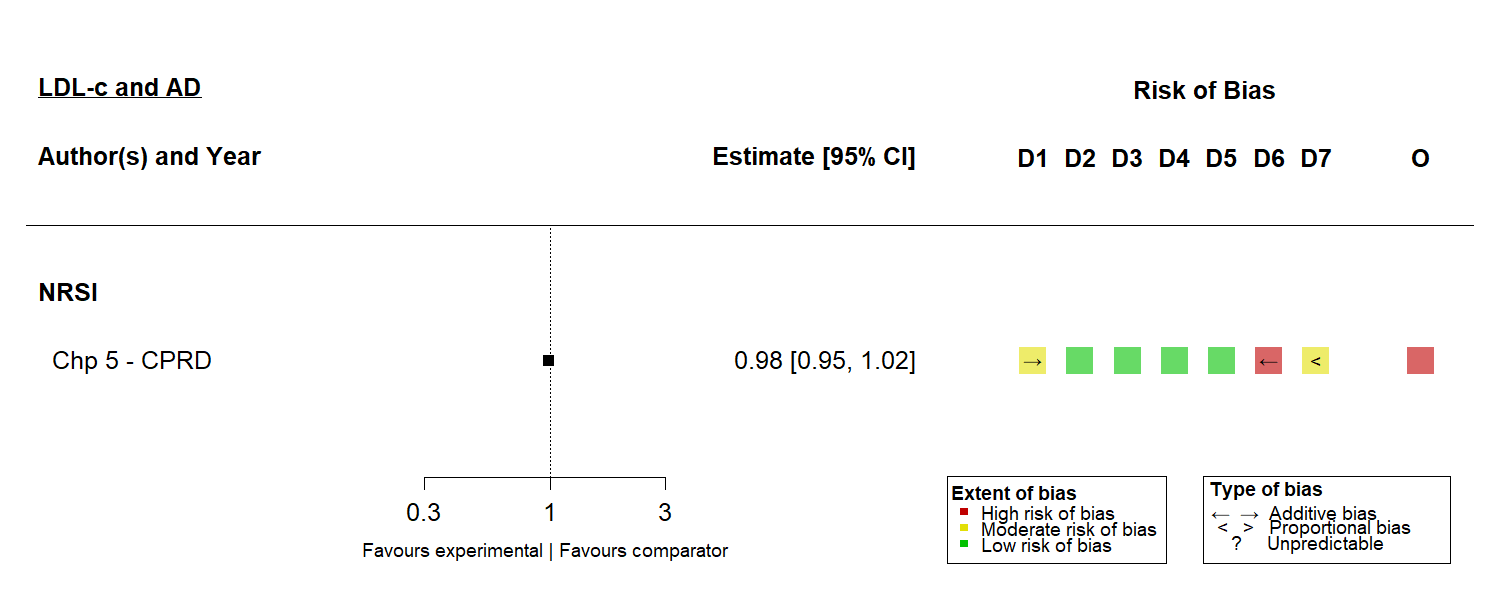
\includegraphics[width=1\linewidth]{figures/tri/midlife_AD_single} \caption[Bias direction plot for a single study]{Bias direction plot for a single study showing the predicted direction of bias in each domain. Additive biases are characterised using arrows, while the proportional biases are denoted using \(<\) and \(>\). A question mark indicates that the direction of bias was unpredictable.}\label{fig:biasDirectionSingle}
\end{figure}

~

With respect to indirectness, the result was judged to be a low risk in the population and outcome domains. However, the fact the result refers to the effect of statins, which may have an effect on dementia outcomes through a mechanism other than LDL-c lowering, put it at high risk of indirectness in the intervention/exposure domain.

The unadjusted estimate was 0.98 (95\%CI: 0.95-1.02). After accounting for the biases and indirectness described, the adjusted result was 1.07 (95\%CI: 0.47-2.42).

~

\hypertarget{case-study-1-effect-of-ldl-c-at-midlife-on-alzheimers-disease}{%
\subsubsection{Case study \#1: effect of LDL-c at midlife on Alzheimer's disease}\label{case-study-1-effect-of-ldl-c-at-midlife-on-alzheimers-disease}}

From the data sources identified in Section \ref{tri-data-sources}, I identified 18 results relevant to my first causal question of interest. Most (n=17) were identified via the systematic review,\textsuperscript{\protect\hyperlink{ref-schilling2017}{53},\protect\hyperlink{ref-ostergaard2015}{71},\protect\hyperlink{ref-ancelin2012}{186}--\protect\hyperlink{ref-bettermann2012}{188},\protect\hyperlink{ref-chou2014}{193},\protect\hyperlink{ref-haag2009}{197},\protect\hyperlink{ref-li2004}{201},\protect\hyperlink{ref-li2010}{202},\protect\hyperlink{ref-rea2005}{207},\protect\hyperlink{ref-reitz2010}{209},\protect\hyperlink{ref-smeeth2009}{210},\protect\hyperlink{ref-zandi2005}{216},\protect\hyperlink{ref-tynkkynen2018}{242},\protect\hyperlink{ref-yoshitake1995}{245}} while Chapter \ref{cprd-heading} provided an additional estimate from the CPRD analysis. The extent, type and direction of predicted bias for each result can be seen in the bias-direction plot presented in Figure \ref{fig:ldlAdBiasDirection}, stratified by study design.

~





\begin{figure}[H]
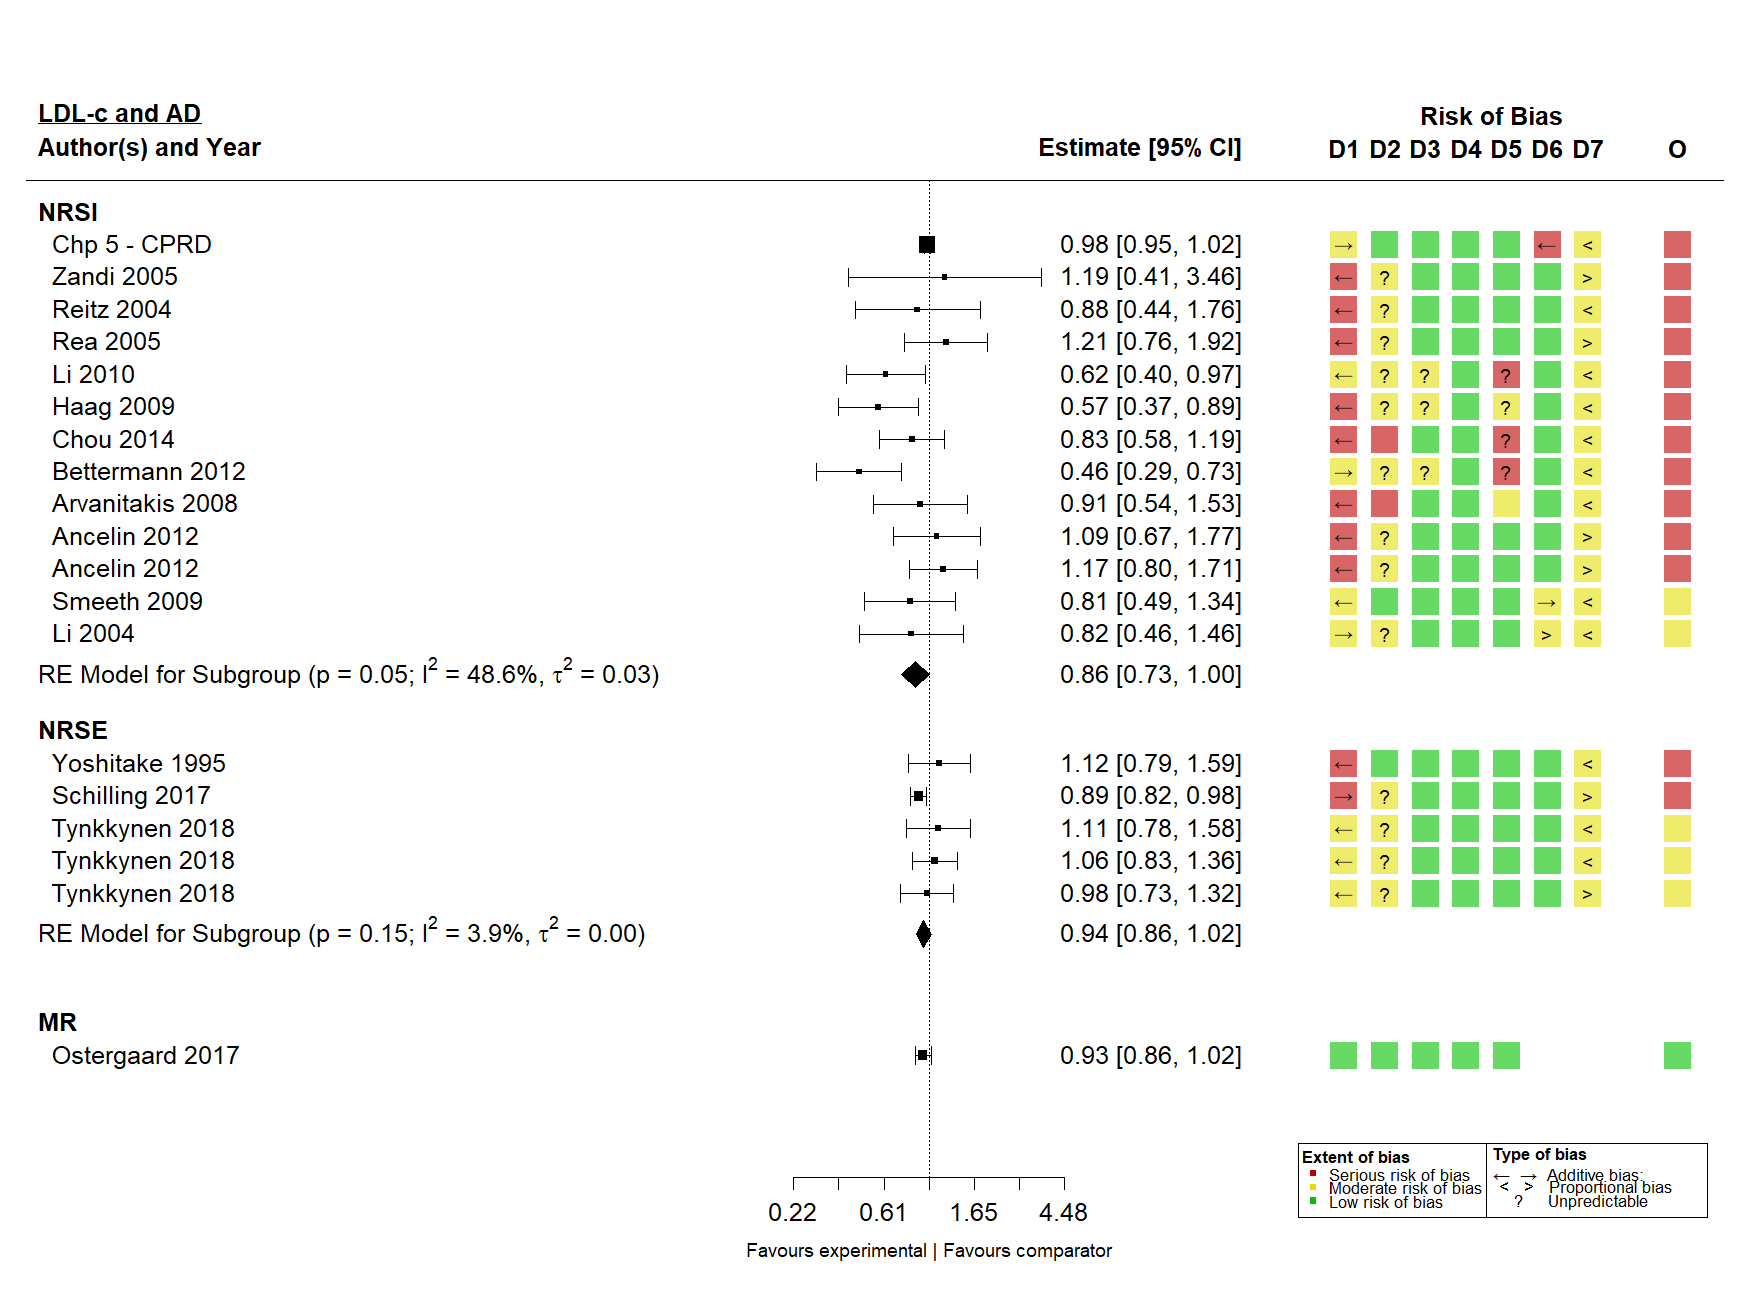
\includegraphics[width=1\linewidth]{figures/tri/midlife_AD} \caption[Bias direction plot, summarising internal biases]{Bias direction plot, summarising the internal biases related to effect of LDL-c on Alzheimer's disease, stratified by study design.}\label{fig:ldlAdBiasDirection}
\end{figure}

~

The results of the unadjusted and the bias-/indirectness-adjusted (under Scenario 1) are shown in Figure \ref{fig:fpLdlAd}. Following adjustment for bias and indirectness, the observed effect attenuates to the null (unadjusted 0.94, 95\%CI: 0.89-0.99; adjusted 0.95, 95\%CI: 0.86-1.04). Additionally, adjustment for bias and indirectness substantially reduced the heterogeneity between studies (unadjusted \(\tau^2\) = 0.0017, \(I^2\) = 17; adjusted \(\tau^2\) = 0, \(I^2\) = 0). However, as can been seen from the right panel in Figure \ref{fig:fpLdlAd}, this reduction in heterogeneity between studies is largely achieved via a reduction in the precision of each individual result.

~





\begin{figure}[H]
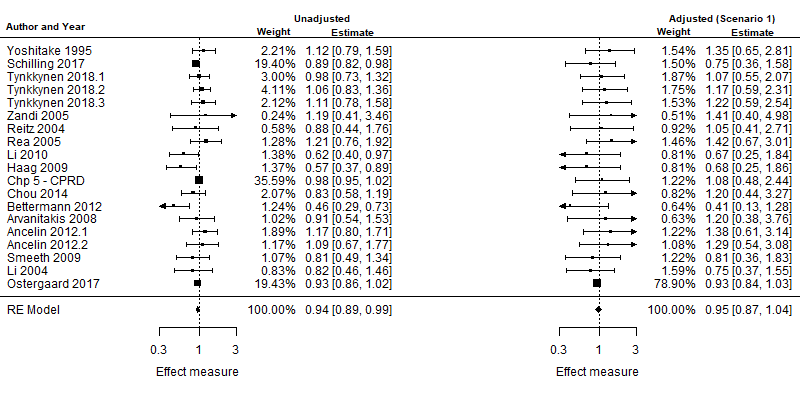
\includegraphics[width=1\linewidth]{figures/tri/fp_paired_midlife_ldl_ad} \caption[Random effects meta-analysis using unadjusted and bias-/indirectness-adjusted results.]{Random effects meta-analysis of the association of midlife LDL-c with Alzheimer's disease, using unadjusted and bias-/indirectness-adjusted results.}\label{fig:fpLdlAd}
\end{figure}

~

The estimates obtained under the two scenarios of additive bias are plotted in Figure \ref{fig:fpLdlAdComparison}, and no substantial differences were observed between the them.





\begin{figure}[H]
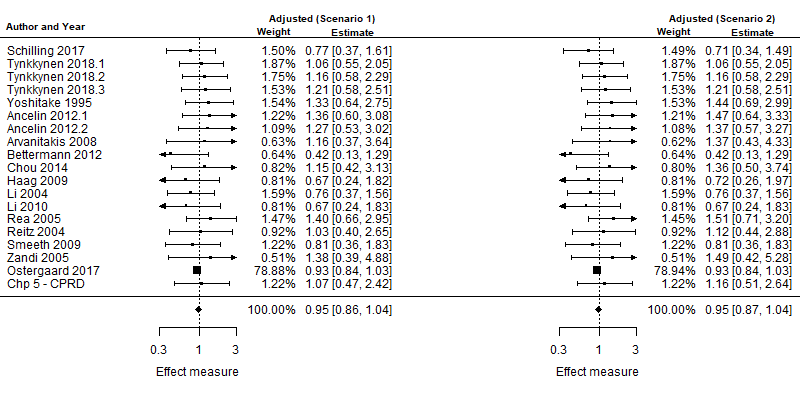
\includegraphics[width=1\linewidth]{figures/tri/fp_paired_midlife_ldl_ad_scenarios} \caption[Comparison of bias-/indirectness-adjusted meta-analyses under two different scenarios of prior distributions of bias.]{Comparison of bias-/indirectness-adjusted meta-analyses of LDL-c/Alzheimer's disease, using two different scenarios for the relationship of levels of bias. The left forest plot shows the result where the difference in mean value between the ``High'' and ``Moderate'' bias levels is the same as between the ``Moderate'' and ``Low'' levels. In the right plot, the difference in mean value between ``High'' and ``Moderate'' is twice that between ``Moderate'' and ``Low''.}\label{fig:fpLdlAdComparison}
\end{figure}

~

\hypertarget{case-study-2-effect-of-triglycerides-at-midlife-on-vascular-dementia}{%
\subsubsection{Case study \#2: effect of triglycerides at midlife on vascular dementia}\label{case-study-2-effect-of-triglycerides-at-midlife-on-vascular-dementia}}

From the data sources identified in Section \ref{tri-data-sources}, I identified 7 results relevant to my causal question of interest: 4 were identified via the systematic review,\textsuperscript{\protect\hyperlink{ref-forti2010}{222},\protect\hyperlink{ref-raffaitin2009}{234},\protect\hyperlink{ref-yoshitake1995}{245}} while Chapter \ref{cprd-heading} provided two additional estimates from unanalysed datasets (CaPS and Whitehall II), and Chapter \ref{ipd-heading} provides an estimate for the effect of fibrates, a treatment for hypertriglyceridaemia. The extent, type and direction of predicted bias for each result can be seen in the bias-direction plot presented in Figure \ref{fig:tgVadBiasDirection}, stratified by study design.





\begin{figure}[H]
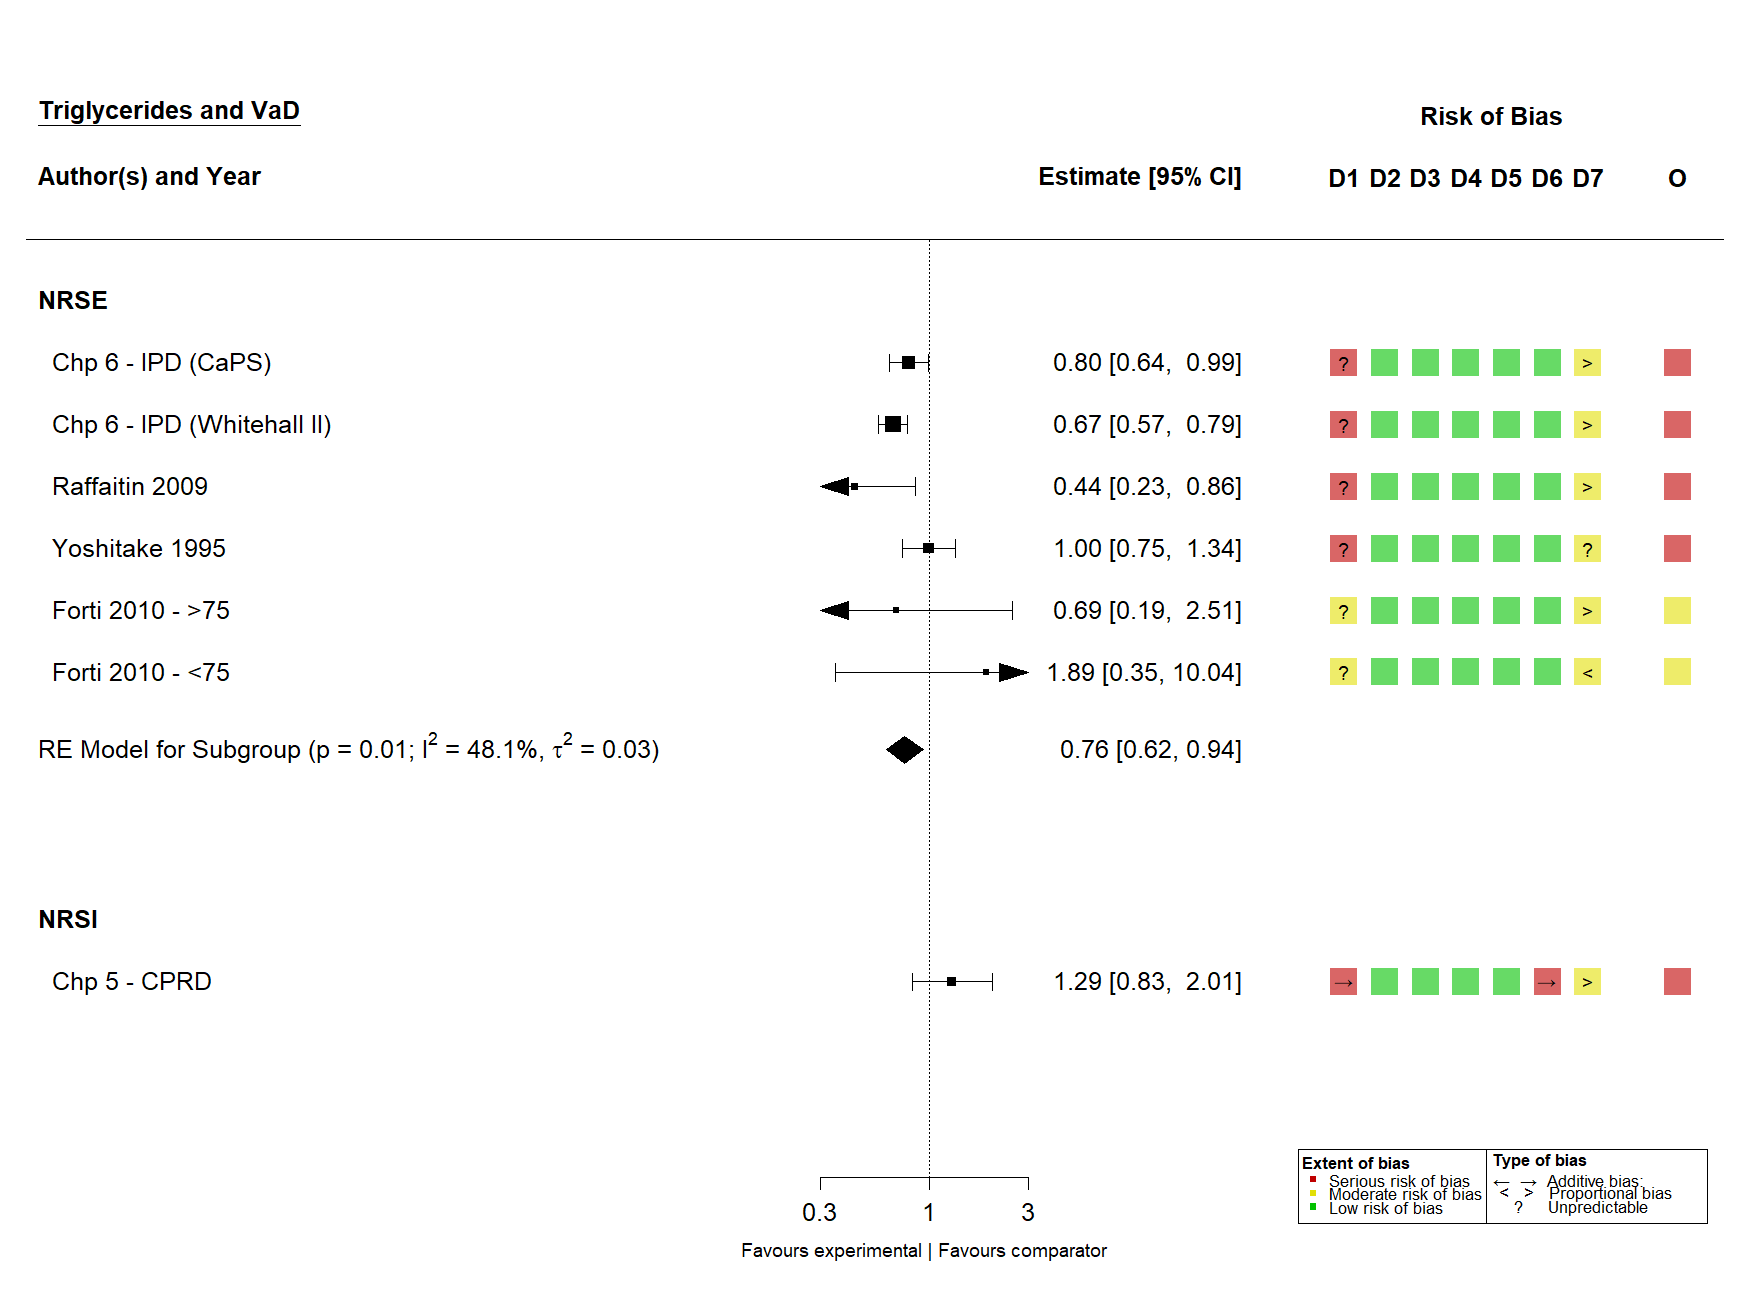
\includegraphics[width=1\linewidth]{figures/tri/midlife_VaD} \caption[shortcap]{Bias direction plot, summarising the internal biases related to effect of triglycerides on vascular dementia, stratified by study design.}\label{fig:tgVadBiasDirection}
\end{figure}

Comparison of the unadjusted and bias-/indirectness-adjusted results for the effect of triglycerides on vascular dementia did not demonstrate a substantial difference (unadjusted 0.82, 95\%CI: 0.64-1.05; adjusted 0.79, 95\%CI: 0.58-1.08; Figure \ref{fig:fpTgVad}), though again, heterogeneity between the adjusted results was greatly reduced (unadjusted \(\tau^2\) = 0.054, \(I^2\) = 65; adjusted \(\tau^2\) = 0, \(I^2\) = 0). Similarly there was minimal difference between the results under the two scenarios of bias (Figure \ref{fig:fpTgVaDComparison})





\begin{figure}[H]
\includegraphics[width=1\linewidth]{figures/tri/fp_paired_midlife_tg_vad} \caption[shortcap]{Random effects meta-analysis of the association of midlife triglycerides and vascular dementia, using unadjusted and bias-/indirectness-adjusted (Scenario 1) results.}\label{fig:fpTgVad}
\end{figure}

~





\begin{figure}[H]
\includegraphics[width=1\linewidth]{figures/tri/fp_paired_midlife_tg_vad_scenarios} \caption[Comparison of bias-/indirectness-adjusted meta-analyses under two different scenarios of prior distributions of bias.]{Comparison of bias-/indirectness-adjusted meta-analyses of triglycerides/vascular dementia, using two different scenarios for the relationship of levels of bias. The left forest plot shows the result where the difference in mean value between the ``High'' and ``Moderate'' bias levels is the same as between the ``Moderate'' and ``Low'' levels. In the right plot, the difference in mean value between ``High'' and ``Moderate'' is twice that between ``Moderate'' and ``Low''.}\label{fig:fpTgVaDComparison}
\end{figure}

\hypertarget{discussion-4}{%
\section{Discussion}\label{discussion-4}}

\hypertarget{summary-of-findings-3}{%
\subsection{Summary of findings}\label{summary-of-findings-3}}

This chapter has narratively synthesised the evidence identified and produced by the previous chapters, highlighting the absence of any consistent association between any blood lipid and any dementia outcome.

In addition, it has sought to provide a generalised framework for quantitative triangulation, building on existing methods for systematic domain-based risk of bias assessment and bias-/indirectness-adjusted meta-analysis. To illustrate the method, I considered two causal questions: the effect of LDL-c at mid-life with Alzheimer's disease and the effect of triglycerides on vascular dementia. In the quantitative triangulation framework, there was very weak evidence for an effect in relation to either of the causal questions considered. The heterogeneity between results produced by different study designs contributing to the analysis was substantially reduced using this method, though this was largely due to a reduction in the precision of each individual result.

~

\hypertarget{limitations-2}{%
\subsection{Limitations}\label{limitations-2}}

The quantitative analysis presented in this chapter is subject to some strong methodological limitation, which are discussed in detail below.

\hypertarget{defining-reasonable-prior-distributions-for-bias-and-indirectness}{%
\subsubsection{Defining reasonable prior distributions for bias and indirectness}\label{defining-reasonable-prior-distributions-for-bias-and-indirectness}}

The key limitation of the quantitative synthesis presented in this chapter is the lack of empirical evidence available for the prior distributions for bias and indirectness. While I attempted to address this by informing the prior distributions using data from a previous expert elicitation exercise, the extent of bias/indirectness in that analysis may not generalise to the one presented here.

Ideally, these prior distributions would be based on empirical data on the effect of different domains of bias/indirectness on a result. Most meta-epidemiological studies examining the effect of different methodological issues studied only randomised controlled trials,\textsuperscript{\protect\hyperlink{ref-amer2021}{348},\protect\hyperlink{ref-page2016}{349}} and the estimates of bias they produce may not hold for non-randomised study designs. However, the prior distributions defined here are broadly comparable to previously reported estimates of the impact of bias in non-randomised trials. For example, a previous simulation study estimated that, in the absence of true effect of LDL-c, ApoE4 would induce a RR of 1.09 with risk of dementia per 1-SD increase in LDL-c.\textsuperscript{\protect\hyperlink{ref-iwagami2021}{350}} This is comparable to the mean assigned to the prior distribution mapped to ``Moderate'' additive bias (N(0.08,0.05), Table \ref{tab:priorsAdd-table}).

A further limitation is the assumption that the distributions of bias are identical across domains of bias. Previous evidence from meta-epidemiological studies of randomised controlled trials that investigated the effects of different biases indicates that this is unlikely to be the case.\textsuperscript{\protect\hyperlink{ref-savovic2018}{351}} The generalised framework for quantitative triangulation, presented here and available via the \texttt{triangulate} package (see Section \ref{tri-software}), allows for domain-specific distributions of bias/indirectness. As more information on the effect of specific sources of bias becomes available, such domain-specific distributions should be used.

Finally, it may in fact be more reasonable for domains such as bias due to confounding to adjust on a per-confounder basis rather than mapping to a ``Moderate'' or ``High'' extent of bias. In this approach, prior distributions are assigned to each of the confounders pre-specified as part of the ROBINS-I/ROBINS-E tools.\textsuperscript{\protect\hyperlink{ref-sterne2016}{157}} Then, rather than assigning a domain level distribution based on an arbitrary judgement of how many important confounders are missing, the result is adjusted for each confounder not accounted for in the original analysis.

~

\hypertarget{accuracy-of-bias-indirectness-assessment}{%
\subsubsection{Accuracy of bias-/indirectness-assessment}\label{accuracy-of-bias-indirectness-assessment}}

A key issue in this analysis is the accuracy of the assessment of bias and indirectness in each result. It has been widely demonstrated that the inter-rater agreement when using risk-of-bias tools is low with regards to the extnet of bias assinged to each domain\textsuperscript{\protect\hyperlink{ref-hartling2011}{352}--\protect\hyperlink{ref-minozzi2020}{354}} Though not previously studied, given the difficulty in assessing the predicted direction of bias, agreement on this aspect of the tools is likely to be lower still.

A further issue in this regard is that rigourness of the tools may not be equivalent. This issue can be illustrated by the Ostergaard \emph{et al.} study\textsuperscript{\protect\hyperlink{ref-ostergaard2015}{71}} having low risk of bias across all domains and thus receiving a substantial proportion of the weight in the first case study (Figure \ref{fig:fpLdlAd}). While the RoB suite of tools (RoB 2.0, ROBINS-I, ROBINS-E) were developed by an expert working group and have been widely used, the Mamluk \emph{et al.} tool\textsuperscript{\protect\hyperlink{ref-mamluk2020}{163}} used to assess risk of bias in Mendelian randomisation studies was designed by the authors for use in their own review. If the Mamluk tool is failing to adequately assess bias in Mendelian randomisation studies, then any analysis based on its assessments is likely to be subject to bias. This observation is particularly problematic given the default position of the ROBINS-I and ROBINS-E tool to require a ``Moderate'' judgement in the confounding domain. Under these conditions, it is possible that a well performed cohort study (low risk of bias across everything other that bias due to confounding) will be down-weighted versus a potentially poor MR study.

~

\hypertarget{low-and-critical-risk-of-bias}{%
\subsubsection{Low and critical risk of bias}\label{low-and-critical-risk-of-bias}}

As illustrated in Table \ref{tab:robLevelsMapping-table}, studies at critical risk of bias were not included in the analysis. While this is in line with best practice, there is theoretically no reason why studies with this extent of bias could not be included in the propsed framework. However, the estimation of an appropriate prior distribution for the effect of ``Critical'' bias would be substantially more challenging, and so was avoided here.

A related issue is the ``Low'' risk of bias judgement. In this analysis, I assumed that domains at ``Low'' risk of bias did not require any adjustment. However, ``Low'' risk of bias is not equivalent to the absence of bias, and potentially should still be adjusted for, if only minimally. In this case, defining the predicted direction of bias would be particularly challenging in the absence of obvious sources of bias.

~

\hypertarget{combination-of-different-effect-measures}{%
\subsubsection{Combination of different effect measures}\label{combination-of-different-effect-measures}}

A final limitation to this analysis is the synthesis of different effect estimates. As discussed in Section \ref{hold}, hazard ratios are not directly comparable to odds ratios, as they inherently account for person time-at-risk.\textsuperscript{\protect\hyperlink{ref-mckenzie2019}{166}} As non-randomised studies (NRSI/NRSI) of dementia outcomes report hazard ratios and Mendelian randomisation studies report odds ratios, the resulting synthesis may be biased by the integration of these two different effect measures.

\textbf{{[}Note: I would be particularly interested in your feedback here. It seems quantitative triangulation will frequently require integration of different effect measures if comparing e.g.~NRSI reporting hazard ratios with MR reporting odds ratios. How should this be handled?{]}}

~

\hypertarget{strengths-2}{%
\subsection{Strengths}\label{strengths-2}}

The core strength of this analysis is that it is based on a comprehensive systematic review, supplemented by two additional primary studies to fill in the identified evidence gaps. In general, triangulation of any sort should be considered a natural extension of evidence synthesis, and therefore should follow best practice in relation to finding and critically assessing all relevant information. Additionally, the approach presented here also builds on recent developments in bias assessment to ``explode out'' the component results of a meta-analysis, and consider the effects of bias/indirectness in each separately.

A further advantage of this method comes from the ability to specify the prior distributions for each level of bias/indirectness in advance of performing the assessments. In previous attempts at bias-/indirectness-adjusted meta-analysis, the extent of bias in each study was assessed via a elicitation process using a panel of methodologists and topic experts.\textsuperscript{\protect\hyperlink{ref-turner2009}{343},\protect\hyperlink{ref-thompson2011}{345},\protect\hyperlink{ref-wilks2011}{355}} However, this approach is potentially subject to differential misclassification of the impact of bias/indirectness on the basis of the results, as there is no way to ensure that results at a similar level of bias for confounding (for example) are being adjusted by the same amount across studies. As an illustrative example, if experts are influenced by the knowledge of the effect estimate in a study, then a result demonstrating a stronger protective effect may receive greater modification than a study at the same ``risk'' of confounding but with a more modest effect. This is likely to be part where experts have preconceived ideas about the true effectiveness of the intervention. In this case, separating the assessment of bias/indirectness from the assignment of modifying values to each judgement will limit the potential for this misclassification. Using the framework proposed, reasonable modifying distributions for each level of bias could be defined \emph{a priori} by the study team using the elicitation procedure detailed previously,\textsuperscript{\protect\hyperlink{ref-turner2009}{343}} similar to how important confounders and co-interventions are defined in advance when performing ROBINS-I/ROBINS-E assessments.\textsuperscript{\protect\hyperlink{ref-sterne2016}{157}}

Finally, accounting for bias using an incorrect prior distribution is no less problematic that synthesising and drawing conclusions from effect estimates as if they were unbiased, a common occurrence in systematic reviews.\textsuperscript{\protect\hyperlink{ref-katikireddi2015}{181}} While this analysis may be limited by the absence of empirically-derived adjustment distributions, it at the very least acknowledges the uncertainty of evidence due to bias/indirectness via a reduction in precision.

~

\newpage

\hypertarget{future-research}{%
\subsection{Future research}\label{future-research}}

An obvious avenue for future work in relation to quantitative triangulation is the identification of empirical prior distributions for the effect of bias/indirectness in non-randomised studies using meta-epidemiological approaches. This will be substantially more challenging than examining the effect of bias in RCTs,\textsuperscript{\protect\hyperlink{ref-savovic2018}{351}} given the absence of an underlying database of meta-analysis of non-randomised studies.

Future development of this framework should also account for bias at the analysis level in terms of missing evidence.\textsuperscript{\protect\hyperlink{ref-zotero-15123}{165}} For example, there is at least one known study relevant to the vascular dementia case study that reported a non-significant result but provided insufficient details to be included in the analysis.\textsuperscript{\protect\hyperlink{ref-chiang2007}{220}} Ideally, a quantitative triangulation framework would further account for this proportional meta-bias (as bias due to missing evidence is most likely to bias away from the null due to publication bias mechanisms), in addition to result-specific biases.

Appreciation that both the risk-of-bias and indirectness of a result should be assessed is growing. Indeed, some existing for the assessment of diagnostic test accuracy\textsuperscript{\protect\hyperlink{ref-whiting2011}{356}} and prediction models\textsuperscript{\protect\hyperlink{ref-moons2019}{357}} consider indirectness (termed applicability in these tools) alongside the assessment of bias. Future iterations of the core risk-of-bias tools (RoB 2, ROBINS-I, ROBINS-E) could take this into account, though there is an competing argument that indirectness is already handled via tools such as the GRADE framework.\textsuperscript{\protect\hyperlink{ref-guyatt2011}{344}} In addition, simple steps like harmonising the risk-of-bias judgements across tools and making the direction of bias question mandatory (even if users default to ``Unpredictable'') would represent an improvement in the tools and encourage users to think about how the biases assessed affect the corresponding result. Similarly, software that implements a risk-of-bias tool should allow for direction/extent of bias question and carefully consider how this data will be exported.

~

\hypertarget{tri-software}{%
\subsection{Outputs}\label{tri-software}}

There are two key outputs from this project. The first is the \texttt{triangulate} R package. Personal communication with the authors of the original method resulted in the STATA code to implement the bias-/indirectness-adjusted model.\textsuperscript{\protect\hyperlink{ref-turner2009}{343}} This has since been generalised as part of the \texttt{triangulate} R package to enable other users to apply the approach detailed here. The package allows for preprocessing of domain-based risk-of-bias data to correctly identify the direction of the bias relative to the effect estimate, use of domain-specific prior distributions, production of bias direction plots (via the tool described in Appendix @ref(?), calculation of bias/indirectness-adjusted estimates for each result, and synthesis of these adjusted results in a standard random-effects meta-analysis.

The second key output is an annotated example dataset for the LDL-c/Alzheimer's disease causal question addressed in this chapter. Available via the \texttt{triangulate} package, this data will provide developers of new triangulation methods with an example dataset on which to test new tools, something which seriously hindered development of this work.

~

\hypertarget{summary-6}{%
\section{Summary}\label{summary-6}}

\begin{itemize}
\item
  In this chapter, I narratively described the evidence identified or produced in previous chapters, and highlighted the issues with a qualitative approach to triangulation when there are several sources of evidence.
\item
  I then illustrated a proposed generalised framework for quantitative triangulation, exploiting existing methods in evidence synthesis and recent developments in the assessment of different risks of bias. I illustrated this method using two case studies: the effect of mid-life LDL-c on Alzheimer's disease, and the effect of mid-life triglycerides on vascular dementia.
\item
  I discussed the limitations of this proposed method, given the absence of informative priors for the impact of bias/indirectness, and proposed future research (i.e.~meta-epidemiological studies) that would address them.
\item
  In summary, quantitative triangulation is a promising field that should be considered a natural extension of evidence synthesis. The implications of the synthesised evidence presented here to clinical practice, public health and future research is considered in the following chapter.
\end{itemize}

\newpage

\hypertarget{references-6}{%
\section{References}\label{references-6}}



\hypertarget{discussion-heading}{%
\chapter{Discussion}\label{discussion-heading}}

\minitoc 

~

\hypertarget{lay-summary-7}{%
\section{Lay summary}\label{lay-summary-7}}

TBC

\hypertarget{introduction-4}{%
\section{Introduction}\label{introduction-4}}

The aim of this thesis was to attempt to infer the causal effect of blood lipid levels on dementia outcomes. In this discussion, I will review the role of each chapter in the broader thesis, summarise the principal findings and contributions of this thesis, and discuss the implications of my findings for both clinical and public health policy. I consider the overall strengths and limitations of this thesis as a coherent body of work, and suggest avenues for impactful future research based on my findings and experiences.

\hypertarget{chapter-summary}{%
\section{Chapter summary}\label{chapter-summary}}

This thesis is comprised of a mix of informative, methodological and applied chapters.

In Chapter \textbf{Chapter \ref{sys-rev-tools-heading}}, I introduced the core concepts considered in thie

In \textbf{Chapter \ref{sys-rev-tools-heading}}, I presented a new tool for the systematic searching of health-related preprints, and detail

In \textbf{Chapters \ref{sys-rev-methods-heading}}, I describe the methods of a comprehensive systematic review of the relationship between dementia outcomes and blood lipids (and treatments that modify them). The results of this analysis are then presented in \textbf{Chapter \ref{sys-rev-results-heading}}.

In \textbf{Chapter \ref{cprd-heading}}, I describe an analysis of lipid-regulating use and dementia outcomes in the CPRD, a large scale electronic health database. I make use of control outcomes to illustrate insufficiently controlled biases

In \textbf{Chapter \ref{ipd-heading}}, I present an individual patient data meta-analysis, using previously unanalysed data accessed via the Dementia Platform UK to add to the evidence base on the association of blood lipids and dementia outcomes.

Finally, in \textbf{Chapter \ref{tri-heading}} I propose a new method of systematically integration of multiple evidence sources as part of quantitative triangulation exercise. I illustrate the method by considering two causal questions (LDL-c and Alzheimer's disease; triglycerides and vascular dementia), drawing on the evidence identified or produced by previous chapters.

~

\hypertarget{summary-of-principle-findings}{%
\section{Summary of principle findings}\label{summary-of-principle-findings}}

Overall, I did not identify a consistent effect of any blood lipid fraction (total cholesterol, LDL cholesterol, HDL cholesterol or triglycerides) on any dementia outcome (all-cause dementia, Alzheimer's disease or vascular dementia).

While published non-randomised studies provided evidence for a protective effect of statin use on Alzheimer's disease, this effect was not maintained when incorporated along with other sources of evidence in a quantitative triangulation framework. However, this equally may indicate that statins have a pleiotropic effects on Alzheimer's disease, that is an effect other than through lipid-lowering. However, this observed effect could also be due to reporting biases, a

The inclusion of preprints

Statins were by far the most studied lipid-regulating agent in relation to dementia outcomes, a unsurprising finding given the large proportion of patients taking statins as indicated by my analysis of the CPRD data.

The inclusion

~

\hypertarget{new-evidence}{%
\section{New evidence}\label{new-evidence}}

Since the systematic review described in this thesis was performed, there have been two notable analysis of large cohorts performed related to the central thesis question here. Two of these are discussed here notable studies are discussed here.

The first a large scale analysis of blood lipids in the CPRD, which found a slight raised risk of dementia in CPRD patients () with higher LDL-c measured at mid-life, driven by the finding for Alzheimer's disease.\textsuperscript{\protect\hyperlink{ref-iwagami2021}{350}} These findings are consistent with the findings presented in this thesis, particularly given the lack of adjustment for confounding by ApoE4.

The UKBioBank is a\textsuperscript{\protect\hyperlink{ref-sudlow2015}{359}}

A recent analysis of 502,226 participants of this found no association between lipids at mid-life and dementia outcomes (women: TC HR: 1.04, 95\%CI: 0.99-1.09, HDL HR: 0.95, 95\%CI: 0.83-1.10, LDL HR: 1.06, 95\%CI: 1.00-1.13/men: TC HR: 0.98, 95\%CI: 0.93-1.03, HDL HR: 1.10, 95\%CI: 0.95-1.29, LDL HR: 0.97, 95\%CI: 0.91-1.04).\textsuperscript{\protect\hyperlink{ref-gong2021}{360}} Results were boardly similar between the all-cause dementia, Alzheimer's disease and vascular dementia outcomes. This is comparable to my findings.

~

\hypertarget{summary-of-contributions}{%
\section{Summary of contributions}\label{summary-of-contributions}}

The research described in this thesis represents a number of novel contributions to the the fields of evidence synthesis

With respect to dementia epidemiology, the systematic review reported in Chapters

~

\hypertarget{lessons-learned}{%
\section{Lessons learned}\label{lessons-learned}}

As a reflective process throughout the PhD, I maintained a catalogue of failures available in Appendix \ref{appendix-catalogue-failures}, describing . here I present a more general rel

In hindsight, the decision to take a broad approach to inclusion of dementia outcomes potentially resulted in larger workload than anticipated, particularly when considered evidence from across different study designs. In a do-over, I would have considered a single dementia outcome.

Additionally, in hindsight, I may have considered a more methodological thesis. The Chapter's I enjoyed working on the most (Chapters @ref())

Further, a more aggressive approach to , Potential approaches could have included sending emails via my supervisors

However, normal opportunities to tie people down in person were suspended during COVID.

~

\hypertarget{overall-strengths-and-limitations}{%
\section{Overall strengths and limitations}\label{overall-strengths-and-limitations}}

The strengths a limitations of each component of this thesis have been discussed in the respective chapters. Here I highlight the strengths and weakness of the thesis as a body of work.

~

\hypertarget{strengths-3}{%
\subsubsection{Strengths}\label{strengths-3}}

This thesis has used multiple sources of evidence to examine the relationship between blood lipids levels and cholesterol risk in a systematic manner, including diverse sources of evidence, inclu

It has highlighted the importance of including preprints in systematic review, and provided a tool to enable researchers to easily do so.

It has provided new evidence on an understudied condition (vascular demenita), analysing three previously unexplored datasets to provide evinde

\begin{itemize}
\tightlist
\item
  New evidence sources for an under-studied condition
\item
  Development of new methods and tool
\end{itemize}

One particularly strength is the lengths gone to find all available published and unpublished evidence around the question, and to integrate this evidence in a coherent framework, taking into account the limitations of ach source and how these limitations may be used to provide

~

\hypertarget{weaknessess}{%
\subsubsection{Weaknessess}\label{weaknessess}}

However, the thesis as a whole is subject to some strong limitations.

A general limitation of this thesis is the absence of known results/data. This occurred in both the systematic review, via the selection of reporting results and potential for publication bias. It was also observed.

Similarly, missing evidence was a common theme across this thesis. In Chapters \ref{hold}/\ref{hold}, several studies stated that they did not report the results of an analysis because the results were not significant. This was particularly common among non-randomised studies of exposure examining blood lipids directly. Fortunately, new tools such as the forthcoming ROB-ME.

Similarly, an absence of evidence on vascular dementia limits the certainty. In both these cases, accounting for missing evidence will be an important part of future evidence snythesis work on this topic.

Missing evidence in the form of a poor response to data access requests was also observed in the IPD analysis reported in Chapter \ref{hold}.

A final weakness of this thesis is the geographical focus. All primary analysis presented drew on data from the UK population (CPRD, CaPS, EPIC Norfolk, Whitehall II).

~

\hypertarget{implications-of-this-research}{%
\section{Implications of this research}\label{implications-of-this-research}}

\hypertarget{clinical-practice}{%
\subsection{Clinical practice}\label{clinical-practice}}

This should focus on doctors being honesty with patients from the outset and describing what they know regarding the uncertainty of the evidence.

While also recognising that the impact of statin or other LRA use on dementia is going to be secondary to their established effect on lipid-lowering. To even be at risk of developing dementia, patients must survive to old-age, something that is substantially less likely given uncontolled hypercholesterolaemia.

The clinical recommendations that can be drawn from the work in this thesis are limited, due to the low strength of evidence. Across multiple sources of evidence, there was no consistent effect of blood lipids on dementia outcomes.

However, even under the scenario that a strong protective effect was identified, whether or not to prescribed a statin at mid-life will always be guided by factors other than dementia prevention. Patients must live to a certain age in order to be at risk of dementia (with the exception of familial early onset dementias), which is substantially less likely if hypercholesterolemia is left unchecked.

However, while this thesis did not provide any evidence for a protective effect of lipid-lowering, it similarly did not provide any evidence for a harmful effect of statin exposure on dementia outcomes.

There was very we. Conversely however, there was an absence of evidence for a harmful effect of statins on. Given the reality that given the choice, given the conflicting evidence

As with many many studies of dementia outcomes, a key limiting factor of any analysis is the absence of a detailed pathological mechanism for the condition. It could well be that statins do have a true effect independently of lipid levels, though based on the certainty of evidence in NRSI, this is unlikely.

~

\hypertarget{public-health}{%
\subsection{Public health}\label{public-health}}

This section should

The absence of an effect of blood lipids on dementia outcomes is an unh

However, future work

~

\hypertarget{reproducible-research}{%
\section{Reproducible research}\label{reproducible-research}}

Reproducible and science has been a key theme running through this thesis, as reflected by the development of an open source tool to help search medRxiv and bioRxiv preprint metadata. In line with this, an open source copy of the code used to produce this thesis is available on GitHub, as is the code used to perform the analysis contained within it.

Unfortunately, given the. However, as discussed in other chapters of this thesis and elsewhere, sharing of analysis code is a useful step towards transparency when the underlying datasets are not readily available.

Commentary on the fact that the best you can do is replicate vs reproducible (due the closed nature of the data).

One is the ability to recreate the results given the same data and code, the other is the ability to recreate the results given the same code but a different dataset. IN theory it is possible to gain access the dataset given the information presented in Chapter @(ref:cprd-analysis-heading). However, access is dependency on an ISAC application to the managing body of the CPRD.

~

\hypertarget{future-work-1}{%
\section{Future work}\label{future-work-1}}

Several avenues for future research, building on the work presented here, are possible.

\hypertarget{inclusion-of-preprints-1}{%
\subsection{Inclusion of preprints}\label{inclusion-of-preprints-1}}

Given the evidence that this thesis produced on the usefulness of including preprints, normalisation of inclusion of preprints in systematic reviews. Wider assessment of the evidence base that exists solely as preprinted literature ()

Meta-epidemiological studies examining the factors which influence eventual publication would also help to quantify the extent and strength of publication bias

Preprints also represent a key opportunity to assess the impact of peer review on qualitative changes within

Future work should also address how to handle discrepancies between the preprinted and published versions of a paper, particularly if the results are subtantially different between the two versions.

~

\hypertarget{evidence-on-vascular-dementia}{%
\subsection{Evidence on vascular dementia}\label{evidence-on-vascular-dementia}}

As discussed in an earlier section, there is an absence of evidence on vascular dementia across the evidence base

Future work should aim to address this evidence gap.

large-scale GWAS of vascular dementia should be performed, to identify associated loci that future Mendelian randomisation studies can make use of. While this is methodologically challenging, given the difficult in diagnosing ``pure'' vascular dementia, it would be a worthwhile endeavour, and would allow for the assessment of many genetically driven risk factors beyond those considered in this thesis.

This is particularly relevant given that there was some evidence for an association of hypertriglyceraemia with vascular dementia. Future research should explicitly examine this relationship as part of wider exploration of vascular disease.

~

\hypertarget{reviewing-mendelian-randomisation-studies}{%
\subsection{Reviewing Mendelian randomisation studies}\label{reviewing-mendelian-randomisation-studies}}

As noted in previous chapters, evidence synthesis theory and methods have not been sufficient developed for the inclusion of Mendelian randomisation studies.

A key issue arises from the lack of an established risk of bias tool, limiting future work that requires systematic risk-of-bias assessment, such as the triangulation framework presented in Chapter \ref{hold}. In addition, a lack of guidance around whether the inclusion of two-sample Mendelian randomisation studies using identical summary statistics. This was illustrated in detail in Chapter \ref{4}, where XXX studies using the same , and meta-analysing these as independent effect estimates would provide an overly precise result. Finally, future work should aim to validate search strategies for this study design, paying particular attention to the range of terms used to define it (e.g.~genetic instrumental variable analysis).

Synthesis of Mendelian randomisation studies is not helped by the varied (and often poor) reporting, though the recent release of the STROBE-MR reporting guidelines should go someway to addressing this.

~

\hypertarget{empirical-estimates-of-bias}{%
\subsection{Empirical estimates of bias}\label{empirical-estimates-of-bias}}

Finally, substantial future work should be directed towards the conduct of meta-epidemiological studies to assess the impact of different bias in non-observational studies. While frameworks such as the one employed in Chapter \ref{tri-heading} exist to allow for the production of bias-adjusted and triangulated estimates.

~

\hypertarget{triangulation}{%
\subsection{Triangulation}\label{triangulation}}

It is customary at this point to recommend that a large scale. However, based on the evidence described. In addition, logistical challenges in relation

In summary, there is a need to make better use of the existing evidence accounting for the

The field of quantitative triangulation is one ripe for future work.

In the first instance, guidance

Finally, accounting for bias (and indirectness, if considering causal effects rather than a summary of the literature) is essentially in the interpretation of published literature. While this can take many forms, from the stratification of forest plots by overall risk of bias level, to the or to the more advance bias adjustment approach detailed here, it is insufficient to draw clinical recommendations from meta-analysis that treat effect estimates as if they were unbiased.

~

\hypertarget{overall-conclusions}{%
\section{Overall conclusions}\label{overall-conclusions}}

The

In addition, I have created

and proposed a novel combination of existing methods in pursuit of a generalised quantitative framework.

This thesis has made unique and novel contributions to the

Illustrating that commonly employed approaches to address

Blood lipids

\begin{savequote}
Lasciate ogne speranza, voi ch'intrate. . .
\end{savequote}

\hypertarget{bibliography}{%
\chapter{Bibliography}\label{bibliography}}

\hypertarget{refs}{}
\begin{CSLReferences}{0}{0}
\leavevmode\hypertarget{ref-alzheimer1907}{}%
\CSLLeftMargin{1. }
\CSLRightInline{Alzheimer, A. Uber eine eigenartige {Erkrankung} der {Hirnrinde}. \emph{Zentralbl. Nervenh. Psych.} \textbf{18}, 177--179 (1907).}

\leavevmode\hypertarget{ref-stelzmann1995}{}%
\CSLLeftMargin{2. }
\CSLRightInline{Stelzmann, R. A., Norman Schnitzlein, H. \& Reed Murtagh, F. An english translation of alzheimer's 1907 paper, {`über eine eigenartige erkankung der hirnrinde'}. \emph{Clinical Anatomy} \textbf{8}, 429--431 (1995).}

\leavevmode\hypertarget{ref-edition2013}{}%
\CSLLeftMargin{3. }
\CSLRightInline{Edition, F. \& others. Diagnostic and statistical manual of mental disorders. \emph{Am Psychiatric Assoc} \textbf{21}, (2013).}

\leavevmode\hypertarget{ref-cerejeira2012}{}%
\CSLLeftMargin{4. }
\CSLRightInline{Cerejeira, J., Lagarto, L. \& Mukaetova-Ladinska, E. B. Behavioral and {Psychological Symptoms} of {Dementia}. \emph{Frontiers in Neurology} \textbf{3}, (2012).}

\leavevmode\hypertarget{ref-kumar2013}{}%
\CSLLeftMargin{5. }
\CSLRightInline{Kumar, C. S. \& Kuriakose, J. R. End-of-life care issues in advanced dementia. \emph{Mental Health in Family Medicine} \textbf{10}, 129--132 (2013).}

\leavevmode\hypertarget{ref-burns2009}{}%
\CSLLeftMargin{6. }
\CSLRightInline{Burns, A. \& Iliffe, S. Dementia. \emph{BMJ} \textbf{338}, b75 (2009).}

\leavevmode\hypertarget{ref-robinson2015}{}%
\CSLLeftMargin{7. }
\CSLRightInline{Robinson, L., Tang, E. \& Taylor, J.-P. Dementia: Timely diagnosis and early intervention. \emph{BMJ} \textbf{350}, h3029 (2015).}

\leavevmode\hypertarget{ref-iadecola2013}{}%
\CSLLeftMargin{8. }
\CSLRightInline{Iadecola, C. The pathobiology of vascular dementia. \emph{Neuron} \textbf{80}, (2013).}

\leavevmode\hypertarget{ref-venkat2015}{}%
\CSLLeftMargin{9. }
\CSLRightInline{Venkat, P., Chopp, M. \& Chen, J. Models and {Mechanisms} of {Vascular Dementia}. \emph{Experimental neurology} \textbf{272}, 97--108 (2015).}

\leavevmode\hypertarget{ref-custodio2017}{}%
\CSLLeftMargin{10. }
\CSLRightInline{Custodio, N. \emph{et al.} Mixed dementia: A review of the evidence. \emph{Dementia \& Neuropsychologia} \textbf{11}, 364--370 (2017).}

\leavevmode\hypertarget{ref-sheehan2012}{}%
\CSLLeftMargin{11. }
\CSLRightInline{Sheehan, B. Assessment scales in dementia. \emph{Therapeutic Advances in Neurological Disorders} \textbf{5}, 349--358 (2012).}

\leavevmode\hypertarget{ref-dubois2007}{}%
\CSLLeftMargin{12. }
\CSLRightInline{Dubois, B. \emph{et al.} Research criteria for the diagnosis of {Alzheimer}'s disease: Revising the {NINCDS}{{ADRDA}} criteria. \emph{The Lancet Neurology} \textbf{6}, 734--746 (2007).}

\leavevmode\hypertarget{ref-roman1993}{}%
\CSLLeftMargin{13. }
\CSLRightInline{Román, G. C. \emph{et al.} Vascular dementia: Diagnostic criteria for research studies: Report of the {NINDS}-{AIREN International Workshop}. \emph{Neurology} \textbf{43}, 250--250 (1993).}

\leavevmode\hypertarget{ref-prince2016}{}%
\CSLLeftMargin{14. }
\CSLRightInline{Prince, M. \emph{et al.} Recent global trends in the prevalence and incidence of dementia, and survival with dementia. \emph{Alzheimer's Research \& Therapy} \textbf{8}, 23 (2016).}

\leavevmode\hypertarget{ref-flier2005}{}%
\CSLLeftMargin{15. }
\CSLRightInline{Flier, W. M. van der \& Scheltens, P. Epidemiology and risk factors of dementia. \emph{Journal of Neurology, Neurosurgery \& Psychiatry} \textbf{76}, v2--v7 (2005).}

\leavevmode\hypertarget{ref-baker2019}{}%
\CSLLeftMargin{16. }
\CSLRightInline{Baker, C., Jarrett, T. \& Powell, T. \emph{Dementia: Policy, services and statistics overview}. (2019).}

\leavevmode\hypertarget{ref-wittenberg2019}{}%
\CSLLeftMargin{17. }
\CSLRightInline{Wittenberg, R. \emph{et al.} The costs of dementia in {England}. \emph{International Journal of Geriatric Psychiatry} \textbf{34}, 1095--1103 (2019).}

\leavevmode\hypertarget{ref-prince2014}{}%
\CSLLeftMargin{18. }
\CSLRightInline{Prince, M., Albanese, E., Guerchet, M., Prina, M. \& others. Dementia and risk reduction: An analysis of protective and modifiable factors. \emph{World Alzheimer Report} 66--83 (2014).}

\leavevmode\hypertarget{ref-cummings2020}{}%
\CSLLeftMargin{19. }
\CSLRightInline{Cummings, J., Lee, G., Ritter, A., Sabbagh, M. \& Zhong, K. Alzheimer's disease drug development pipeline: 2020. \emph{Alzheimer's \& Dementia: Translational Research \& Clinical Interventions} \textbf{6}, e12050 (2020).}

\leavevmode\hypertarget{ref-hampel2018}{}%
\CSLLeftMargin{20. }
\CSLRightInline{Hampel, H. \emph{et al.} The cholinergic system in the pathophysiology and treatment of {Alzheimer}'s disease. \emph{Brain} \textbf{141}, 1917--1933 (2018).}

\leavevmode\hypertarget{ref-pariente2008}{}%
\CSLLeftMargin{21. }
\CSLRightInline{Pariente, A. \emph{et al.} Prevalence of cholinesterase inhibitors in subjects with dementia in {Europe}. \emph{Pharmacoepidemiology and Drug Safety} \textbf{17}, 655--660 (2008).}

\leavevmode\hypertarget{ref-marucci2020}{}%
\CSLLeftMargin{22. }
\CSLRightInline{Marucci, G. \emph{et al.} Efficacy of acetylcholinesterase inhibitors in {Alzheimer}'s disease. \emph{Neuropharmacology} 108352 (2020). doi:\href{https://doi.org/10.1016/j.neuropharm.2020.108352}{10.1016/j.neuropharm.2020.108352}}

\leavevmode\hypertarget{ref-francis2010}{}%
\CSLLeftMargin{23. }
\CSLRightInline{Francis, P. T., Ramírez, M. J. \& Lai, M. K. Neurochemical basis for symptomatic treatment of {Alzheimer}'s disease. \emph{Neuropharmacology} \textbf{59}, 221--229 (2010).}

\leavevmode\hypertarget{ref-winblad2016}{}%
\CSLLeftMargin{24. }
\CSLRightInline{Winblad, B. \emph{et al.} Defeating {Alzheimer}'s disease and other dementias: A priority for {European} science and society. \emph{The Lancet Neurology} \textbf{15}, 455--532 (2016).}

\leavevmode\hypertarget{ref-feingold2000}{}%
\CSLLeftMargin{25. }
\CSLRightInline{Feingold, K. R. Introduction to {Lipids} and {Lipoproteins}. in \emph{Endotext} (eds. Feingold, K. R. et al.) ({MDText.com, Inc.}, 2000).}

\leavevmode\hypertarget{ref-peters2019}{}%
\CSLLeftMargin{26. }
\CSLRightInline{Peters, R. \emph{et al.} Combining modifiable risk factors and risk of dementia: A systematic review and meta-analysis. \emph{BMJ Open} \textbf{9}, e022846 (2019).}

\leavevmode\hypertarget{ref-anstey2019}{}%
\CSLLeftMargin{27. }
\CSLRightInline{Anstey, K. J., Ee, N., Eramudugolla, R., Jagger, C. \& Peters, R. A {Systematic Review} of {Meta}-{Analyses} that {Evaluate Risk Factors} for {Dementia} to {Evaluate} the {Quantity}, {Quality}, and {Global Representativeness} of {Evidence}. \emph{Journal of Alzheimer's Disease} \textbf{70}, S165--S186 (2019).}

\leavevmode\hypertarget{ref-hughes2020}{}%
\CSLLeftMargin{28. }
\CSLRightInline{Hughes, D. \emph{et al.} Association of blood pressure lowering with incident dementia or cognitive impairment: A systematic review and meta-analysis. \emph{Jama} \textbf{323}, 1934--1944 (2020).}

\leavevmode\hypertarget{ref-norton2014potential}{}%
\CSLLeftMargin{29. }
\CSLRightInline{Norton, S., Matthews, F. E., Barnes, D. E., Yaffe, K. \& Brayne, C. Potential for primary prevention of {Alzheimer}'s disease: An analysis of population-based data. \emph{The Lancet Neurology} \textbf{13}, 788--794 (2014).}

\leavevmode\hypertarget{ref-pushpakom2019}{}%
\CSLLeftMargin{30. }
\CSLRightInline{Pushpakom, S. \emph{et al.} Drug repurposing: Progress, challenges and recommendations. \emph{Nature Reviews Drug Discovery} \textbf{18}, 41--58 (2019).}

\leavevmode\hypertarget{ref-laufs2020}{}%
\CSLLeftMargin{31. }
\CSLRightInline{Laufs, U., Parhofer, K. G., Ginsberg, H. N. \& Hegele, R. A. Clinical review on triglycerides. \emph{European Heart Journal} \textbf{41}, 99--109c (2020).}

\leavevmode\hypertarget{ref-zampelas2019}{}%
\CSLLeftMargin{32. }
\CSLRightInline{Zampelas, A. \& Magriplis, E. New {Insights} into {Cholesterol Functions}: A {Friend} or an {Enemy}? \emph{Nutrients} \textbf{11}, (2019).}

\leavevmode\hypertarget{ref-friedewald1972}{}%
\CSLLeftMargin{33. }
\CSLRightInline{Friedewald, W. T., Levy, R. I. \& Fredrickson, D. S. Estimation of the {Concentration} of {Low}-{Density Lipoprotein Cholesterol} in {Plasma}, {Without Use} of the {Preparative Ultracentrifuge}. \emph{Clinical Chemistry} \textbf{18}, 499--502 (1972).}

\leavevmode\hypertarget{ref-national2002third}{}%
\CSLLeftMargin{34. }
\CSLRightInline{Detection, N. C. E. P. (US). E. P. on. \emph{Third report of the {National Cholesterol Education Program} ({NCEP}) {Expert Panel} on detection, evaluation, and treatment of high blood cholesterol in adults ({Adult Treatment Panel III})}. ({The Program}, 2002).}

\leavevmode\hypertarget{ref-nelson2013}{}%
\CSLLeftMargin{35. }
\CSLRightInline{Nelson, R. H. Hyperlipidemia as a {Risk Factor} for {Cardiovascular Disease}. \emph{Primary care} \textbf{40}, 195--211 (2013).}

\leavevmode\hypertarget{ref-libby2019}{}%
\CSLLeftMargin{36. }
\CSLRightInline{Libby, P. \emph{et al.} Atherosclerosis. \emph{Nature Reviews Disease Primers} \textbf{5}, 1--18 (2019).}

\leavevmode\hypertarget{ref-collins2016}{}%
\CSLLeftMargin{37. }
\CSLRightInline{Collins, R. \emph{et al.} Interpretation of the evidence for the efficacy and safety of statin therapy. \emph{The Lancet} \textbf{388}, 2532--2561 (2016).}

\leavevmode\hypertarget{ref-law2003}{}%
\CSLLeftMargin{38. }
\CSLRightInline{Law, M. R., Wald, N. J. \& Rudnicka, A. R. Quantifying effect of statins on low density lipoprotein cholesterol, ischaemic heart disease, and stroke: Systematic review and meta-analysis. \emph{BMJ} \textbf{326}, 1423 (2003).}

\leavevmode\hypertarget{ref-schachter2005}{}%
\CSLLeftMargin{39. }
\CSLRightInline{Schachter, M. Chemical, pharmacokinetic and pharmacodynamic properties of statins: An update. \emph{Fundamental \& Clinical Pharmacology} \textbf{19}, 117--125 (2005).}

\leavevmode\hypertarget{ref-sierra2011}{}%
\CSLLeftMargin{40. }
\CSLRightInline{Sierra, S. \emph{et al.} Statins as neuroprotectants: A comparative in vitro study of lipophilicity, blood-brain-barrier penetration, lowering of brain cholesterol, and decrease of neuron cell death. \emph{Journal of Alzheimer's disease: JAD} \textbf{23}, 307--318 (2011).}

\leavevmode\hypertarget{ref-kosoglou2005}{}%
\CSLLeftMargin{41. }
\CSLRightInline{Kosoglou, T. \emph{et al.} Ezetimibe: A review of its metabolism, pharmacokinetics and drug interactions. \emph{Clinical Pharmacokinetics} \textbf{44}, 467--494 (2005).}

\leavevmode\hypertarget{ref-genest2006}{}%
\CSLLeftMargin{42. }
\CSLRightInline{Genest, J. Combination of statin and ezetimibe for the treatment of dyslipidemias and the prevention of coronary artery disease. \emph{The Canadian Journal of Cardiology} \textbf{22}, 863--867 (2006).}

\leavevmode\hypertarget{ref-chaudhary2017}{}%
\CSLLeftMargin{43. }
\CSLRightInline{Chaudhary, R., Garg, J., Shah, N. \& Sumner, A. {PCSK9} inhibitors: A new era of lipid lowering therapy. \emph{World Journal of Cardiology} \textbf{9}, 76--91 (2017).}

\leavevmode\hypertarget{ref-mckenney2004}{}%
\CSLLeftMargin{44. }
\CSLRightInline{McKenney, J. New perspectives on the use of niacin in the treatment of lipid disorders. \emph{Archives of internal medicine} \textbf{164}, 697--705 (2004).}

\leavevmode\hypertarget{ref-skulas2019}{}%
\CSLLeftMargin{45. }
\CSLRightInline{Skulas-Ray Ann C. \emph{et al.} Omega-3 {Fatty Acids} for the {Management} of {Hypertriglyceridemia}: A {Science Advisory From} the {American Heart Association}. \emph{Circulation} \textbf{140}, e673--e691 (2019).}

\leavevmode\hypertarget{ref-burns2003}{}%
\CSLLeftMargin{46. }
\CSLRightInline{Burns, M. P. \emph{et al.} Co-localization of cholesterol, apolipoprotein {E} and fibrillar {A\(\beta\)} in amyloid plaques. \emph{Molecular Brain Research} \textbf{110}, 119--125 (2003).}

\leavevmode\hypertarget{ref-mizuno1999}{}%
\CSLLeftMargin{47. }
\CSLRightInline{Mizuno, T. \emph{et al.} Cholesterol-dependent {Generation} of a {Seeding Amyloid} {\(\beta\)}-{Protein} in {Cell Culture} *. \emph{Journal of Biological Chemistry} \textbf{274}, 15110--15114 (1999).}

\leavevmode\hypertarget{ref-beecham2014}{}%
\CSLLeftMargin{48. }
\CSLRightInline{Beecham, G. W. \emph{et al.} Genome-{Wide Association Meta}-analysis of {Neuropathologic Features} of {Alzheimer}'s {Disease} and {Related Dementias}. \emph{PLoS Genetics} \textbf{10}, (2014).}

\leavevmode\hypertarget{ref-harold2009}{}%
\CSLLeftMargin{49. }
\CSLRightInline{Harold, D. \emph{et al.} Genome-wide association study identifies variants at {CLU} and {PICALM} associated with {Alzheimer}'s disease, and shows evidence for additional susceptibility genes. \emph{Nature genetics} \textbf{41}, 1088--1093 (2009).}

\leavevmode\hypertarget{ref-meng2007}{}%
\CSLLeftMargin{50. }
\CSLRightInline{Meng, Y. \emph{et al.} Association between {SORL1} and {Alzheimer} disease in a genome-wide study. \emph{Neuroreport} \textbf{18}, 1761--1764 (2007).}

\leavevmode\hypertarget{ref-kivipelto2002}{}%
\CSLLeftMargin{51. }
\CSLRightInline{Kivipelto, M. \emph{et al.} Apolipoprotein {E} {\(E\)}4 {Allele}, {Elevated Midlife Total Cholesterol Level}, and {High Midlife Systolic Blood Pressure Are Independent Risk Factors} for {Late}-{Life Alzheimer Disease}. \emph{Annals of Internal Medicine} \textbf{137}, 149--155 (2002).}

\leavevmode\hypertarget{ref-kivipelto2005}{}%
\CSLLeftMargin{52. }
\CSLRightInline{Kivipelto, M. \emph{et al.} Obesity and vascular risk factors at midlife and the risk of dementia and {Alzheimer} disease. \emph{Archives of Neurology} \textbf{62}, 1556--1560 (2005).}

\leavevmode\hypertarget{ref-schilling2017}{}%
\CSLLeftMargin{53. }
\CSLRightInline{Schilling, S. \emph{et al.} Differential associations of plasma lipids with incident dementia and dementia subtypes in the {3C Study}: A longitudinal, population-based prospective cohort study. \emph{PLoS medicine} \textbf{14}, e1002265 (2017).}

\leavevmode\hypertarget{ref-solomon2009}{}%
\CSLLeftMargin{54. }
\CSLRightInline{Solomon, A., Kivipelto, M., Wolozin, B., Zhou, J. \& Whitmer, R. A. Midlife {Serum Cholesterol} and {Increased Risk} of {Alzheimer}'s and {Vascular Dementia Three Decades Later}. \emph{Dementia and Geriatric Cognitive Disorders} \textbf{28}, 75--80 (2009).}

\leavevmode\hypertarget{ref-whitmer2005}{}%
\CSLLeftMargin{55. }
\CSLRightInline{Whitmer, R. A., Sidney, S., Selby, J., Johnston, S. C. \& Yaffe, K. Midlife cardiovascular risk factors and risk of dementia in late life. \emph{Neurology} \textbf{64}, 277--281 (2005).}

\leavevmode\hypertarget{ref-li2005}{}%
\CSLLeftMargin{56. }
\CSLRightInline{Li, G. \emph{et al.} Serum cholesterol and risk of {Alzheimer} disease: A community-based cohort study. \emph{Neurology} \textbf{65}, 1045--1050 (2005).}

\leavevmode\hypertarget{ref-mainous2005}{}%
\CSLLeftMargin{57. }
\CSLRightInline{Mainous, A. G., Eschenbach, S. L., Wells, B. J., Everett, C. J. \& Gill, J. M. Cholesterol, transferrin saturation, and the development of dementia and {Alzheimer}'s disease: Results from an 18-year population-based cohort. \emph{Family Medicine} \textbf{37}, 36--42 (2005).}

\leavevmode\hypertarget{ref-mielke2010}{}%
\CSLLeftMargin{58. }
\CSLRightInline{Mielke, M. M. \emph{et al.} The 32-year relationship between cholesterol and dementia from midlife to late life. \emph{Neurology} \textbf{75}, 1888--1895 (2010).}

\leavevmode\hypertarget{ref-tan2003}{}%
\CSLLeftMargin{59. }
\CSLRightInline{Tan, Z. S. \emph{et al.} Plasma {Total Cholesterol Level} as a {Risk Factor} for {Alzheimer Disease}: The {Framingham Study}. \emph{Archives of Internal Medicine} \textbf{163}, 1053 (2003).}

\leavevmode\hypertarget{ref-mielke2005}{}%
\CSLLeftMargin{60. }
\CSLRightInline{Mielke, M. M. \emph{et al.} High total cholesterol levels in late life associated with a reduced risk of dementia. \emph{Neurology} \textbf{64}, 1689--1695 (2005).}

\leavevmode\hypertarget{ref-reitz2004}{}%
\CSLLeftMargin{61. }
\CSLRightInline{Reitz, C., Tang, M.-X., Luchsinger, J. \& Mayeux, R. Relation of plasma lipids to {Alzheimer} disease and vascular dementia. \emph{Archives of Neurology} \textbf{61}, 705--714 (2004).}

\leavevmode\hypertarget{ref-moroney1999}{}%
\CSLLeftMargin{62. }
\CSLRightInline{Moroney, J. T. Low-{Density Lipoprotein Cholesterol} and the {Risk} of {Dementia With Stroke}. \emph{JAMA} \textbf{282}, 254 (1999).}

\leavevmode\hypertarget{ref-ritchie2015}{}%
\CSLLeftMargin{63. }
\CSLRightInline{Ritchie, C. W., Terrera, G. M. \& Quinn, T. J. Dementia trials and dementia tribulations: Methodological and analytical challenges in dementia research. \emph{Alzheimer's Research \& Therapy} \textbf{7}, 31 (2015).}

\leavevmode\hypertarget{ref-mcguinness2016}{}%
\CSLLeftMargin{64. }
\CSLRightInline{McGuinness, B., Craig, D., Bullock, R. \& Passmore, P. Statins for the prevention of dementia. \emph{The Cochrane Database of Systematic Reviews} CD003160 (2016). doi:\href{https://doi.org/10.1002/14651858.CD003160.pub3}{10.1002/14651858.CD003160.pub3}}

\leavevmode\hypertarget{ref-trompet2010}{}%
\CSLLeftMargin{65. }
\CSLRightInline{Trompet, S. \emph{et al.} Pravastatin and cognitive function in the elderly. {Results} of the {PROSPER} study. \emph{Journal of Neurology} \textbf{257}, 85--90 (2010).}

\leavevmode\hypertarget{ref-heartprotectionstudycollaborativegroup2002}{}%
\CSLLeftMargin{66. }
\CSLRightInline{{MRC}/{BHF Heart Protection Study} of cholesterol lowering with simvastatin in 20 536 high-risk individuals: A randomised placebocontrolled trial. \emph{The Lancet} \textbf{360}, 7--22 (2002).}

\leavevmode\hypertarget{ref-daveysmith2014}{}%
\CSLLeftMargin{67. }
\CSLRightInline{Davey Smith, G. \& Hemani, G. Mendelian randomization: Genetic anchors for causal inference in epidemiological studies. \emph{Human Molecular Genetics} \textbf{23}, R89--R98 (2014).}

\leavevmode\hypertarget{ref-greenland2000}{}%
\CSLLeftMargin{68. }
\CSLRightInline{Greenland, S. An introduction to instrumental variables for epidemiologists. \emph{International Journal of Epidemiology} \textbf{29}, 722--729 (2000).}

\leavevmode\hypertarget{ref-davies2018}{}%
\CSLLeftMargin{69. }
\CSLRightInline{Davies, N. M., Holmes, M. V. \& Smith, G. D. Reading {Mendelian} randomisation studies: A guide, glossary, and checklist for clinicians. \emph{BMJ} \textbf{362}, k601 (2018).}

\leavevmode\hypertarget{ref-larsson2017}{}%
\CSLLeftMargin{70. }
\CSLRightInline{Larsson, S. C. \emph{et al.} Modifiable pathways in {Alzheimer}'s disease: Mendelian randomisation analysis. \emph{BMJ} \textbf{359}, (2017).}

\leavevmode\hypertarget{ref-ostergaard2015}{}%
\CSLLeftMargin{71. }
\CSLRightInline{Østergaard, S. D. \emph{et al.} Associations between {Potentially Modifiable Risk Factors} and {Alzheimer Disease}: A {Mendelian Randomization Study}. \emph{PLOS Medicine} \textbf{12}, e1001841 (2015).}

\leavevmode\hypertarget{ref-kim2009}{}%
\CSLLeftMargin{72. }
\CSLRightInline{Kim, J., Basak, J. M. \& Holtzman, D. M. The {Role} of {Apolipoprotein E} in {Alzheimer}'s {Disease}. \emph{Neuron} \textbf{63}, 287--303 (2009).}

\leavevmode\hypertarget{ref-benn2017}{}%
\CSLLeftMargin{73. }
\CSLRightInline{Benn, M., Nordestgaard, B. G., Frikke-Schmidt, R. \& Tybjærg-Hansen, A. Low {LDL} cholesterol, {PCSK9} and {HMGCR} genetic variation, and risk of {Alzheimer}'s disease and {Parkinson}'s disease: Mendelian randomisation study. \emph{BMJ} \textbf{357}, j1648 (2017).}

\leavevmode\hypertarget{ref-donnelly2018}{}%
\CSLLeftMargin{74. }
\CSLRightInline{Donnelly, C. A. \emph{et al.} Four principles to make evidence synthesis more useful for policy. \emph{Nature} \textbf{558}, 361--364 (2018).}

\leavevmode\hypertarget{ref-chandler2019chapter}{}%
\CSLLeftMargin{75. }
\CSLRightInline{Chandler, J., Higgins, J., Deeks, J., Davenport, C. \& Clarke, M. J. Chapter 1: introduction. in \emph{Cochrane {Handbook} for {Systematic Reviews} of {Interventions} version 6.2 (updated {February} 2021)} \textbf{5}, ({Cochrane}, 2020).}

\leavevmode\hypertarget{ref-conn2003}{}%
\CSLLeftMargin{76. }
\CSLRightInline{Conn, V. S., Valentine, J. C., Cooper, H. M. \& Rantz, M. J. Grey literature in meta-analyses. \emph{Nursing Research} \textbf{52}, 256--261 (2003 Jul-Aug).}

\leavevmode\hypertarget{ref-mcauley2000}{}%
\CSLLeftMargin{77. }
\CSLRightInline{McAuley, L., Pham, B., Tugwell, P. \& Moher, D. Does the inclusion of grey literature influence estimates of intervention effectiveness reported in meta-analyses? \emph{Lancet (London, England)} \textbf{356}, 1228--1231 (2000).}

\leavevmode\hypertarget{ref-hopewell2007}{}%
\CSLLeftMargin{78. }
\CSLRightInline{Hopewell, S., McDonald, S., Clarke, M. \& Egger, M. Grey literature in meta-analyses of randomized trials of health care interventions. \emph{The Cochrane Database of Systematic Reviews} MR000010 (2007). doi:\href{https://doi.org/10.1002/14651858.MR000010.pub3}{10.1002/14651858.MR000010.pub3}}

\leavevmode\hypertarget{ref-lefebvre2019searching}{}%
\CSLLeftMargin{79. }
\CSLRightInline{Lefebvre, C. \emph{et al.} Chapter 4: Searching for and selecting studies. in \emph{Cochrane {Handbook} for {Systematic Reviews} of {Interventions} version 6.2 (updated {February} 2021)} 67--107 ({Cochrane}, 2020).}

\leavevmode\hypertarget{ref-committeeonpublicationethicscope2018}{}%
\CSLLeftMargin{80. }
\CSLRightInline{Committee on Publication Ethics (COPE). \emph{Discussion {Document}: preprints}. (2018).}

\leavevmode\hypertarget{ref-vale2016}{}%
\CSLLeftMargin{81. }
\CSLRightInline{Vale, R. D. \& Hyman, A. A. Priority of discovery in the life sciences. \emph{eLife} \textbf{5}, e16931 (2016).}

\leavevmode\hypertarget{ref-fraser2020preprinting}{}%
\CSLLeftMargin{82. }
\CSLRightInline{Fraser, N. \emph{et al.} Preprinting a pandemic: The role of preprints in the {COVID}-19 pandemic. \emph{bioRxiv} 2020.05.22.111294 (2020). doi:\href{https://doi.org/10.1101/2020.05.22.111294}{10.1101/2020.05.22.111294}}

\leavevmode\hypertarget{ref-rosenthal1979}{}%
\CSLLeftMargin{83. }
\CSLRightInline{Rosenthal, R. The file drawer problem and tolerance for null results. \emph{Psychological Bulletin} \textbf{86}, 638--641 (1979).}

\leavevmode\hypertarget{ref-maslove2018}{}%
\CSLLeftMargin{84. }
\CSLRightInline{Maslove, D. M. Medical {Preprints}{{A Debate Worth Having}}. \emph{JAMA} \textbf{319}, 443--444 (2018).}

\leavevmode\hypertarget{ref-schalkwyk2020}{}%
\CSLLeftMargin{85. }
\CSLRightInline{Schalkwyk, M. C. I. van, Hird, T. R., Maani, N., Petticrew, M. \& Gilmore, A. B. The perils of preprints. \emph{BMJ} \textbf{370}, m3111 (2020).}

\leavevmode\hypertarget{ref-mahood2014}{}%
\CSLLeftMargin{86. }
\CSLRightInline{Mahood, Q., Eerd, D. V. \& Irvin, E. Searching for grey literature for systematic reviews: Challenges and benefits. \emph{Research Synthesis Methods} \textbf{5}, 221--234 (2014).}

\leavevmode\hypertarget{ref-shi2021}{}%
\CSLLeftMargin{87. }
\CSLRightInline{Shi, X. \emph{et al.} Assessment of {Concordance} and {Discordance Among Clinical Studies Posted} as {Preprints} and {Subsequently Published} in {High}-{Impact Journals}. \emph{JAMA Network Open} \textbf{4}, e212110 (2021).}

\leavevmode\hypertarget{ref-klein2019}{}%
\CSLLeftMargin{88. }
\CSLRightInline{Klein, M., Broadwell, P., Farb, S. E. \& Grappone, T. Comparing published scientific journal articles to their pre-print versions. \emph{International Journal on Digital Libraries} \textbf{20}, 335--350 (2019).}

\leavevmode\hypertarget{ref-nicholson2021}{}%
\CSLLeftMargin{89. }
\CSLRightInline{Nicholson, D. N. \emph{et al.} Linguistic {Analysis} of the {bioRxiv Preprint Landscape}. \emph{bioRxiv} 2021.03.04.433874 (2021). doi:\href{https://doi.org/10.1101/2021.03.04.433874}{10.1101/2021.03.04.433874}}

\leavevmode\hypertarget{ref-lawlor2016}{}%
\CSLLeftMargin{90. }
\CSLRightInline{Lawlor, D. A., Tilling, K. \& Davey Smith, G. Triangulation in aetiological epidemiology. \emph{International Journal of Epidemiology} \textbf{45}, 1866--1886 (2016).}

\leavevmode\hypertarget{ref-munafo2018}{}%
\CSLLeftMargin{91. }
\CSLRightInline{Munafò, M. R. \& Smith, G. D. Robust research needs many lines of evidence. \emph{Nature} \textbf{553}, 399--401 (2018).}

\leavevmode\hypertarget{ref-page2021}{}%
\CSLLeftMargin{92. }
\CSLRightInline{Page, M. J. \emph{et al.} The {PRISMA} 2020 statement: An updated guideline for reporting systematic reviews. \emph{BMJ} \textbf{372}, n71 (2021).}

\leavevmode\hypertarget{ref-sterne2019}{}%
\CSLLeftMargin{93. }
\CSLRightInline{Sterne, J. A. C. \emph{et al.} {RoB} 2: A revised tool for assessing risk of bias in randomised trials. \emph{BMJ} \textbf{366}, (2019).}

\leavevmode\hypertarget{ref-mcguinness2018}{}%
\CSLLeftMargin{94. }
\CSLRightInline{McGuinness, L. A., Higgins, J. P. T. \& Sterne, J. A. C. Assessing the {Credibility} of {Findings From Nonrandomized Studies} of {Interventions}. \emph{JAMA Cardiology} \textbf{3}, 905--906 (2018).}

\leavevmode\hypertarget{ref-riley2010}{}%
\CSLLeftMargin{95. }
\CSLRightInline{Riley, R. D., Lambert, P. C. \& Abo-Zaid, G. Meta-analysis of individual participant data: Rationale, conduct, and reporting. \emph{BMJ} \textbf{340}, c221 (2010).}

\leavevmode\hypertarget{ref-stewart1993}{}%
\CSLLeftMargin{96. }
\CSLRightInline{Stewart, L. A. \& Parmar, M. K. B. Meta-analysis of the literature or of individual patient data: Is there a difference? \emph{The Lancet} \textbf{341}, 418--422 (1993).}

\leavevmode\hypertarget{ref-arain2009}{}%
\CSLLeftMargin{97. }
\CSLRightInline{Arain, F. A., Kuniyoshi, F. H., Abdalrhim, A. D. \& Miller, V. M. Sex/gender medicine. {The} biological basis for personalized care in cardiovascular medicine. \emph{Circulation Journal: Official Journal of the Japanese Circulation Society} \textbf{73}, 1774--1782 (2009).}

\leavevmode\hypertarget{ref-clayton2018}{}%
\CSLLeftMargin{98. }
\CSLRightInline{Clayton, J. A. Applying the new {SABV} (sex as a biological variable) policy to research and clinical care. \emph{Physiology \& Behavior} \textbf{187}, 2--5 (2018).}

\leavevmode\hypertarget{ref-mccartney2016}{}%
\CSLLeftMargin{99. }
\CSLRightInline{McCartney, M., Treadwell, J., Maskrey, N. \& Lehman, R. Making evidence based medicine work for individual patients. \emph{BMJ} \textbf{353}, i2452 (2016).}

\leavevmode\hypertarget{ref-letenneur1999}{}%
\CSLLeftMargin{100. }
\CSLRightInline{Letenneur, L. \emph{et al.} Are sex and educational level independent predictors of dementia and {Alzheimer}'s disease? Incidence data from the {PAQUID} project. \emph{Journal of Neurology, Neurosurgery \& Psychiatry} \textbf{66}, 177--183 (1999).}

\leavevmode\hypertarget{ref-riley2020}{}%
\CSLLeftMargin{101. }
\CSLRightInline{Riley, R. D. \emph{et al.} Individual participant data meta-analysis to examine interactions between treatment effect and participant-level covariates: Statistical recommendations for conduct and planning. \emph{Statistics in Medicine} \textbf{39}, 2115--2137 (2020).}

\leavevmode\hypertarget{ref-stewart2002}{}%
\CSLLeftMargin{102. }
\CSLRightInline{Stewart, L. A. \& Tierney, J. F. To {IPD} or not to {IPD}?: Advantages and {Disadvantages} of {Systematic Reviews Using Individual Patient Data}. \emph{Evaluation \& the Health Professions} \textbf{25}, 76--97 (2002).}

\leavevmode\hypertarget{ref-tugwell2010}{}%
\CSLLeftMargin{103. }
\CSLRightInline{Tugwell, P. \& Knottnerus, J. A. Advantages of individual patient data analysis in systematic reviews. \emph{Journal of Clinical Epidemiology} \textbf{63}, 233--234 (2010).}

\leavevmode\hypertarget{ref-nevitt2017}{}%
\CSLLeftMargin{104. }
\CSLRightInline{Nevitt, S. J. \emph{et al.} Exploring changes over time and characteristics associated with data retrieval across individual participant data meta-analyses: Systematic review. \emph{BMJ} \textbf{357}, j1390 (2017).}

\leavevmode\hypertarget{ref-ventresca2020}{}%
\CSLLeftMargin{105. }
\CSLRightInline{Ventresca, M. \emph{et al.} Obtaining and managing data sets for individual participant data meta-analysis: Scoping review and practical guide. \emph{BMC Medical Research Methodology} \textbf{20}, 113 (2020).}

\leavevmode\hypertarget{ref-alsheikh-ali2011}{}%
\CSLLeftMargin{106. }
\CSLRightInline{Alsheikh-Ali, A. A., Qureshi, W., Al-Mallah, M. H. \& Ioannidis, J. P. A. Public {Availability} of {Published Research Data} in {High}-{Impact Journals}. \emph{PLoS ONE} \textbf{6}, e24357 (2011).}

\leavevmode\hypertarget{ref-federer2018}{}%
\CSLLeftMargin{107. }
\CSLRightInline{Federer, L. M. \emph{et al.} Data sharing in {PLOS ONE}: An analysis of {Data Availability Statements}. \emph{PLOS ONE} \textbf{13}, e0194768 (2018).}

\leavevmode\hypertarget{ref-vines2014}{}%
\CSLLeftMargin{108. }
\CSLRightInline{Vines, T. H. \emph{et al.} The {Availability} of {Research Data Declines Rapidly} with {Article Age}. \emph{Current Biology} \textbf{24}, 94--97 (2014).}

\leavevmode\hypertarget{ref-vanpanhuis2014}{}%
\CSLLeftMargin{109. }
\CSLRightInline{van Panhuis, W. G. \emph{et al.} A systematic review of barriers to data sharing in public health. \emph{BMC Public Health} \textbf{14}, 1144 (2014).}

\leavevmode\hypertarget{ref-wartenberg2010}{}%
\CSLLeftMargin{110. }
\CSLRightInline{Wartenberg, D. \& Thompson, W. D. Privacy {Versus Public Health}: The {Impact} of {Current Confidentiality Rules}. \emph{American Journal of Public Health} \textbf{100}, 407--412 (2010).}

\leavevmode\hypertarget{ref-bauermeister2020}{}%
\CSLLeftMargin{111. }
\CSLRightInline{Bauermeister, S. \emph{et al.} The {Dementias Platform UK} ({DPUK}) {Data Portal}. \emph{European Journal of Epidemiology} \textbf{35}, 601--611 (2020).}

\leavevmode\hypertarget{ref-rawlinson2019}{}%
\CSLLeftMargin{112. }
\CSLRightInline{Rawlinson, C. \& Bloom, T. New preprint server for medical research. \emph{BMJ} \textbf{365}, (2019).}

\leavevmode\hypertarget{ref-sever2019}{}%
\CSLLeftMargin{113. }
\CSLRightInline{Sever, R. \emph{et al.} \emph{{bioRxiv}: The preprint server for biology}. ({Scientific Communication and Education}, 2019). doi:\href{https://doi.org/10.1101/833400}{10.1101/833400}}

\leavevmode\hypertarget{ref-beely2013}{}%
\CSLLeftMargin{114. }
\CSLRightInline{Bealy, C. R {Programming Humour}. \emph{Stack Exchange} (2013).}

\leavevmode\hypertarget{ref-bramer2018}{}%
\CSLLeftMargin{115. }
\CSLRightInline{Bramer, W. M., de Jonge, G. B., Rethlefsen, M. L., Mast, F. \& Kleijnen, J. A systematic approach to searching: An efficient and complete method to develop literature searches. \emph{Journal of the Medical Library Association : JMLA} \textbf{106}, 531--541 (2018).}

\leavevmode\hypertarget{ref-gusenbauer2020}{}%
\CSLLeftMargin{116. }
\CSLRightInline{Gusenbauer, M. \& Haddaway, N. R. Which academic search systems are suitable for systematic reviews or meta-analyses? Evaluating retrieval qualities of {Google Scholar}, {PubMed}, and 26 other resources. \emph{Research Synthesis Methods} \textbf{11}, 181--217 (2020).}

\leavevmode\hypertarget{ref-zotero-15029}{}%
\CSLLeftMargin{117. }
\CSLRightInline{Ropensci/medrxivr: Access and search {medRxiv} and {bioRxiv} preprint data.}

\leavevmode\hypertarget{ref-wateridge1995}{}%
\CSLLeftMargin{118. }
\CSLRightInline{Wateridge, J. {IT} projects: A basis for success. \emph{International Journal of Project Management} \textbf{13}, 169--172 (1995).}

\leavevmode\hypertarget{ref-abdill2019}{}%
\CSLLeftMargin{119. }
\CSLRightInline{Abdill, R. J. \& Blekhman, R. Rxivist.org: Sorting biology preprints using social media and readership metrics. \emph{PLOS Biology} \textbf{17}, e3000269 (2019).}

\leavevmode\hypertarget{ref-zotero-15027}{}%
\CSLLeftMargin{120. }
\CSLRightInline{Rxivist: Explore popular biology preprints.}

\leavevmode\hypertarget{ref-iwema2016}{}%
\CSLLeftMargin{121. }
\CSLRightInline{Iwema, C. L., LaDue, J., Zack, A. \& Chattopadhyay, A. Search.{bioPreprint}: A discovery tool for cutting edge, preprint biomedical research articles. \emph{F1000Research} \textbf{5}, 1396 (2016).}

\leavevmode\hypertarget{ref-shaw2002}{}%
\CSLLeftMargin{122. }
\CSLRightInline{Shaw, M. "{Self}-healing": Softening precision to avoid brittleness: Position paper for {WOSS} '02: Workshop on self-healing systems. \emph{Proceedings of the first workshop on Self-healing systems} 111--114 (2002). doi:\href{https://doi.org/10.1145/582128.582152}{10.1145/582128.582152}}

\leavevmode\hypertarget{ref-laprie1992}{}%
\CSLLeftMargin{123. }
\CSLRightInline{Laprie, J. C. Dependability: Basic {Concepts} and {Terminology}. in \emph{Dependability: Basic {Concepts} and {Terminology}: In {English}, {French}, {German}, {Italian} and {Japanese}} (ed. Laprie, J. C.) 3--245 ({Springer}, 1992).}

\leavevmode\hypertarget{ref-rcoreteam2019}{}%
\CSLLeftMargin{124. }
\CSLRightInline{R Core Team. \emph{R: A language and environment for statistical computing}. ({R Foundation for Statistical Computing}, 2019).}

\leavevmode\hypertarget{ref-zotero-15031}{}%
\CSLLeftMargin{125. }
\CSLRightInline{Git scraping: Track changes over time by scraping to a {Git} repository.}

\leavevmode\hypertarget{ref-rethlefsen2021prisma}{}%
\CSLLeftMargin{126. }
\CSLRightInline{Rethlefsen, M. L. \emph{et al.} {PRISMA}-{S}: An extension to the {PRISMA} statement for reporting literature searches in systematic reviews. \emph{Systematic reviews} \textbf{10}, 1--19 (2021).}

\leavevmode\hypertarget{ref-kodvanj2020}{}%
\CSLLeftMargin{127. }
\CSLRightInline{Kodvanj, I., Homolak, J., Virag, D. \& Trkulja, V. Publishing of {COVID}-19 {Preprints} in {Peer}-reviewed {Journals}, {Preprinting Trends}, {Public Discussion} and {Quality Issues}. \emph{bioRxiv} 2020.11.23.394577 (2020). doi:\href{https://doi.org/10.1101/2020.11.23.394577}{10.1101/2020.11.23.394577}}

\leavevmode\hypertarget{ref-noone2020}{}%
\CSLLeftMargin{128. }
\CSLRightInline{Noone, C. \emph{et al.} Investigating and evaluating evidence of the behavioural determinants of adherence to social distancing measures {} {A} protocol for a scoping review of {COVID}-19 research. \emph{HRB Open Research} \textbf{3}, 46 (2020).}

\leavevmode\hypertarget{ref-grassly2020}{}%
\CSLLeftMargin{129. }
\CSLRightInline{Grassly, N. C. \emph{et al.} Comparison of molecular testing strategies for {COVID}-19 control: A mathematical modelling study. \emph{The Lancet Infectious Diseases} \textbf{20}, 1381--1389 (2020).}

\leavevmode\hypertarget{ref-mcguinness2020DAScomparison}{}%
\CSLLeftMargin{130. }
\CSLRightInline{McGuinness, L. A. \& Sheppard, A. L. A descriptive analysis of the data availability statements accompanying {medRxiv} preprints and a comparison with their published counterparts. \emph{MetaArXiv} (2020). doi:\href{https://doi.org/10.31222/osf.io/p75xe}{10.31222/osf.io/p75xe}}

\leavevmode\hypertarget{ref-boettiger2015}{}%
\CSLLeftMargin{131. }
\CSLRightInline{Boettiger, C., Chamberlain, S., Hart, E. \& Ram, K. Building {Software}, {Building Community}: Lessons from the {rOpenSci Project}. \emph{Journal of Open Research Software} \textbf{3}, e8 (2015).}

\leavevmode\hypertarget{ref-mcguinness2020medrxivr}{}%
\CSLLeftMargin{132. }
\CSLRightInline{McGuinness, L. \& Schmidt, L. Medrxivr: Accessing and searching {medRxiv} and {bioRxiv} preprint data in {R}. \emph{Journal of Open Source Software} \textbf{5}, 2651 (2020).}

\leavevmode\hypertarget{ref-zotero-15016}{}%
\CSLLeftMargin{133. }
\CSLRightInline{Issue \#380 - medrxivr: Accessing and searching {medRxiv} preprint data in {R} {\(\cdot\)} {\(\cdot\)} ropensci/software-review {\(\cdot\)} {GitHub}. \emph{GitHub {\(\cdot\)} ropensci/software-review}}

\leavevmode\hypertarget{ref-abdill2019popularity}{}%
\CSLLeftMargin{134. }
\CSLRightInline{Abdill, R. J. \& Blekhman, R. Tracking the popularity and outcomes of all {bioRxiv} preprints. \emph{eLife} \textbf{8}, e45133 (2019).}

\leavevmode\hypertarget{ref-bong2019}{}%
\CSLLeftMargin{135. }
\CSLRightInline{Bong, S. M., McKay, J. L., Factor, S. A. \& Ting, L. H. \emph{Perception of whole-body motion during balance perturbations is impaired in {Parkinson}'s disease and is associated with balance impairment}. ({Neurology}, 2019). doi:\href{https://doi.org/10.1101/19000265}{10.1101/19000265}}

\leavevmode\hypertarget{ref-song2010}{}%
\CSLLeftMargin{136. }
\CSLRightInline{Song, F. \emph{et al.} Dissemination and publication of research findings: An updated review of related biases. \emph{Health Technology Assessment} \textbf{14}, (2010).}

\leavevmode\hypertarget{ref-goldacre2019}{}%
\CSLLeftMargin{137. }
\CSLRightInline{Goldacre, B., Morton, C. E. \& DeVito, N. J. Why researchers should share their analytic code. \emph{BMJ} l6365 (2019). doi:\href{https://doi.org/10.1136/bmj.l6365}{10.1136/bmj.l6365}}

\leavevmode\hypertarget{ref-mckiernan2016}{}%
\CSLLeftMargin{138. }
\CSLRightInline{McKiernan, E. C. \emph{et al.} How open science helps researchers succeed. \emph{eLife} \textbf{5}, e16800 (2016).}

\leavevmode\hypertarget{ref-fraser2020rbiorixv}{}%
\CSLLeftMargin{139. }
\CSLRightInline{Fraser, N. \emph{Rbiorxiv: Client for the '{bioRxiv}' {API}}. (2020).}

\leavevmode\hypertarget{ref-vuorre2020}{}%
\CSLLeftMargin{140. }
\CSLRightInline{Vuorre, M. \& Crump, M. J. C. Sharing and organizing research products as {R} packages. \emph{Behavior Research Methods} (2020). doi:\href{https://doi.org/10.3758/s13428-020-01436-x}{10.3758/s13428-020-01436-x}}

\leavevmode\hypertarget{ref-cochrane1979}{}%
\CSLLeftMargin{141. }
\CSLRightInline{Cochrane, A. L. 1931-1971: A critical review, with particular reference to the medical profession. \emph{Medicines for the year 2000} (1979).}

\leavevmode\hypertarget{ref-mcguinnessluke2020}{}%
\CSLLeftMargin{142. }
\CSLRightInline{McGuinness, L., Higgins, J., Ben-Shlomo, Yoav, Coulthard, L. \& Smith, G. The relationship between blood lipid levels and dementia: Protocol for a systematic review and triangulation of all available evidence. \emph{OSF} (2020). doi:\href{https://doi.org/10.17605/OSF.IO/VTW5Y}{10.17605/OSF.IO/VTW5Y}}

\leavevmode\hypertarget{ref-organizationwho1993}{}%
\CSLLeftMargin{143. }
\CSLRightInline{Organization(WHO), W. H. \emph{The {ICD}-10 classification of mental and behavioural disorders: Diagnostic criteria for research}. ({World Health Organization}, 1993).}

\leavevmode\hypertarget{ref-greenhalgh2005}{}%
\CSLLeftMargin{144. }
\CSLRightInline{Greenhalgh, T. \& Peacock, R. Effectiveness and efficiency of search methods in systematic reviews of complex evidence: Audit of primary sources. \emph{BMJ : British Medical Journal} \textbf{331}, 1064--1065 (2005).}

\leavevmode\hypertarget{ref-wohlin2014}{}%
\CSLLeftMargin{145. }
\CSLRightInline{Wohlin, C. Guidelines for snowballing in systematic literature studies and a replication in software engineering. in \emph{Proceedings of the 18th {International Conference} on {Evaluation} and {Assessment} in {Software Engineering} - {EASE} '14} 1--10 ({ACM Press}, 2014). doi:\href{https://doi.org/10.1145/2601248.2601268}{10.1145/2601248.2601268}}

\leavevmode\hypertarget{ref-bramer2016}{}%
\CSLLeftMargin{146. }
\CSLRightInline{Bramer, W. M., Giustini, D., de Jonge, G. B., Holland, L. \& Bekhuis, T. De-duplication of database search results for systematic reviews in {EndNote}. \emph{Journal of the Medical Library Association : JMLA} \textbf{104}, 240--243 (2016).}

\leavevmode\hypertarget{ref-hupe2019}{}%
\CSLLeftMargin{147. }
\CSLRightInline{Hupe, M. {EndNote X9}. \emph{Journal of Electronic Resources in Medical Libraries} \textbf{16}, 117--119 (2019).}

\leavevmode\hypertarget{ref-ouzzani2016}{}%
\CSLLeftMargin{148. }
\CSLRightInline{Ouzzani, M., Hammady, H., Fedorowicz, Z. \& Elmagarmid, A. Rayyan-a web and mobile app for systematic reviews. \emph{Systematic Reviews} \textbf{5}, 210 (2016).}

\leavevmode\hypertarget{ref-gwet2008}{}%
\CSLLeftMargin{149. }
\CSLRightInline{Gwet, K. L. Computing inter-rater reliability and its variance in the presence of high agreement. \emph{British Journal of Mathematical and Statistical Psychology} \textbf{61}, 29--48 (2008).}

\leavevmode\hypertarget{ref-cohen1960}{}%
\CSLLeftMargin{150. }
\CSLRightInline{Cohen, J. A {Coefficient} of {Agreement} for {Nominal Scales}. \emph{Educational and Psychological Measurement} \textbf{20}, 37--46 (1960).}

\leavevmode\hypertarget{ref-wongpakaran2013}{}%
\CSLLeftMargin{151. }
\CSLRightInline{Wongpakaran, N., Wongpakaran, T., Wedding, D. \& Gwet, K. L. A comparison of {Cohen}'s {Kappa} and {Gwet}'s {AC1} when calculating inter-rater reliability coefficients: A study conducted with personality disorder samples. \emph{BMC Medical Research Methodology} \textbf{13}, 61 (2013).}

\leavevmode\hypertarget{ref-brennan1992}{}%
\CSLLeftMargin{152. }
\CSLRightInline{Brennan, P. \& Silman, A. Statistical methods for assessing observer variability in clinical measures. \emph{BMJ : British Medical Journal} \textbf{304}, 1491--1494 (1992).}

\leavevmode\hypertarget{ref-mchugh2012}{}%
\CSLLeftMargin{153. }
\CSLRightInline{McHugh, M. L. Interrater reliability: The kappa statistic. \emph{Biochemia Medica} \textbf{22}, 276--282 (2012).}

\leavevmode\hypertarget{ref-higgins2019}{}%
\CSLLeftMargin{154. }
\CSLRightInline{Higgins, J. P., Li, T. \& Deeks, J. J. Section 6.5.2.10 : Combining groups. in \emph{Cochrane {Handbook} for {Systematic Reviews} of {Interventions} version 6.0 (updated {August} 2019)} (eds. Higgins, J. P. T. et al.) ({Cochrane}, 2019).}

\leavevmode\hypertarget{ref-rugge2011}{}%
\CSLLeftMargin{155. }
\CSLRightInline{Rugge, B. \emph{et al.} Appendix {A}: Lipid {Conversion Factors}. in \emph{Screening and {Treatment} of {Subclinical Hypothyroidism} or {Hyperthyroidism}} ({Agency for Healthcare Research and Quality (US)}, 2011).}

\leavevmode\hypertarget{ref-reynders2019}{}%
\CSLLeftMargin{156. }
\CSLRightInline{Reynders, R. M., Ladu, L. \& Girolamo, N. D. Contacting of authors modified crucial outcomes of systematic reviews but was poorly reported, not systematic, and produced conflicting results. \emph{Journal of Clinical Epidemiology} \textbf{115}, 64--76 (2019).}

\leavevmode\hypertarget{ref-sterne2016}{}%
\CSLLeftMargin{157. }
\CSLRightInline{Sterne, J. A. \emph{et al.} {ROBINS}-{I}: A tool for assessing risk of bias in non-randomised studies of interventions. \emph{BMJ} \textbf{355}, i4919 (2016).}

\leavevmode\hypertarget{ref-campbell1957}{}%
\CSLLeftMargin{158. }
\CSLRightInline{Campbell, D. T. Factors relevant to the validity of experiments in social settings. \emph{Psychological Bulletin} \textbf{54}, 297--312 (1957).}

\leavevmode\hypertarget{ref-juni2001}{}%
\CSLLeftMargin{159. }
\CSLRightInline{Jüni, P., Altman, D. G. \& Egger, M. Assessing the quality of controlled clinical trials. \emph{BMJ} \textbf{323}, 42--46 (2001).}

\leavevmode\hypertarget{ref-morganr2020}{}%
\CSLLeftMargin{160. }
\CSLRightInline{Morgan R \emph{et al.} A tool to assess {Risk Of Bias In Non}-randomised {Studies} - of {Exposures} ({ROBINS}-{E}). in \emph{Advances in {Evidence Synthesis}: Special issue, {Cochrane Database} of {Systematic Reviews}} \textbf{9 Supp 1}, 320 (2020).}

\leavevmode\hypertarget{ref-french2019}{}%
\CSLLeftMargin{161. }
\CSLRightInline{French, C. E. \emph{et al.} Cannabis use and the risk of tuberculosis: A systematic review. \emph{BMC Public Health} \textbf{19}, 1006 (2019).}

\leavevmode\hypertarget{ref-wells2000}{}%
\CSLLeftMargin{162. }
\CSLRightInline{Wells, G. A. \emph{et al.} The {Newcastle}-{Ottawa Scale} ({NOS}) for assessing the quality of nonrandomised studies in meta-analyses. (2000).}

\leavevmode\hypertarget{ref-mamluk2020}{}%
\CSLLeftMargin{163. }
\CSLRightInline{Mamluk, L. \emph{et al.} Evidence of detrimental effects of prenatal alcohol exposure on offspring birthweight and neurodevelopment from a systematic review of quasi-experimental studies. \emph{International Journal of Epidemiology} \textbf{49}, 1972--1995 (2020).}

\leavevmode\hypertarget{ref-spiga2021}{}%
\CSLLeftMargin{164. }
\CSLRightInline{Spiga, F. \emph{et al.} Tools for the assessment of quality and risk of bias in {Mendelian} randomization studies: A systematic review. \emph{medRxiv} 2021.10.21.21265126 (2021). doi:\href{https://doi.org/10.1101/2021.10.21.21265126}{10.1101/2021.10.21.21265126}}

\leavevmode\hypertarget{ref-zotero-15123}{}%
\CSLLeftMargin{165. }
\CSLRightInline{Matthew J Page \emph{et al.} \emph{Risk {Of Bias} due to {Missing Evidence} ({ROB}-{ME}): A new tool for assessing risk of non-reporting biases in evidence syntheses - {Detailed} guidance}.}

\leavevmode\hypertarget{ref-mckenzie2019}{}%
\CSLLeftMargin{166. }
\CSLRightInline{McKenzie, J. E. \& Brennan, S. E. Section 12.1: Why a meta-analysis of effect estimates may not be possible. in \emph{Cochrane {Handbook} for {Systematic Reviews} of {Interventions} version 6.0 (updated {August} 2019)} (eds. Higgins, J. P. T. et al.) ({Cochrane}, 2019).}

\leavevmode\hypertarget{ref-vanderweele2020}{}%
\CSLLeftMargin{167. }
\CSLRightInline{VanderWeele, T. J. Optimal approximate conversions of odds ratios and hazard ratios to risk ratios. \emph{Biometrics} \textbf{76}, 746--752 (2020).}

\leavevmode\hypertarget{ref-hedges1998}{}%
\CSLLeftMargin{168. }
\CSLRightInline{Hedges, L. V. \& Vevea, J. L. Fixed-and random-effects models in meta-analysis. \emph{Psychological methods} \textbf{3}, 486 (1998).}

\leavevmode\hypertarget{ref-dersimonian1986}{}%
\CSLLeftMargin{169. }
\CSLRightInline{DerSimonian, R. \& Laird, N. Meta-analysis in clinical trials. \emph{Controlled Clinical Trials} \textbf{7}, 177--188 (1986).}

\leavevmode\hypertarget{ref-deeks2019}{}%
\CSLLeftMargin{170. }
\CSLRightInline{Deeks, J. J., Altman, D. G. \& Higgins, J. P. T. Section 10.11.4: Meta-regression. in \emph{Cochrane {Handbook} for {Systematic Reviews} of {Interventions} version 6.0 (updated {August} 2019)} (eds. Higgins, J. P. T. et al.) ({Cochrane}, 2019).}

\leavevmode\hypertarget{ref-greenland1992}{}%
\CSLLeftMargin{171. }
\CSLRightInline{Greenland, S. \& Longnecker, M. P. Methods for {Trend Estimation} from {Summarized Dose}-{Response Data}, with {Applications} to {Meta}-{Analysis}. \emph{American Journal of Epidemiology} \textbf{135}, 1301--1309 (1992).}

\leavevmode\hypertarget{ref-durrleman1989}{}%
\CSLLeftMargin{172. }
\CSLRightInline{Durrleman, S. \& Simon, R. Flexible regression models with cubic splines. \emph{Statistics in Medicine} \textbf{8}, 551--561 (1989).}

\leavevmode\hypertarget{ref-liu2009}{}%
\CSLLeftMargin{173. }
\CSLRightInline{Liu, Q., Cook, N. R., Bergström, A. \& Hsieh, C.-C. A two-stage hierarchical regression model for meta-analysis of epidemiologic nonlinear dose{}response data. \emph{Computational Statistics \& Data Analysis} \textbf{53}, 4157--4167 (2009).}

\leavevmode\hypertarget{ref-gauthier2020}{}%
\CSLLeftMargin{174. }
\CSLRightInline{Gauthier, J., Wu, Q. V. \& Gooley, T. A. Cubic splines to model relationships between continuous variables and outcomes: A guide for clinicians. \emph{Bone Marrow Transplantation} \textbf{55}, 675--680 (2020).}

\leavevmode\hypertarget{ref-white2009}{}%
\CSLLeftMargin{175. }
\CSLRightInline{White, I. R. Multivariate random-effects meta-analysis. \emph{The Stata Journal} \textbf{9}, 40--56 (2009).}

\leavevmode\hypertarget{ref-gasparrini2012}{}%
\CSLLeftMargin{176. }
\CSLRightInline{Gasparrini, A., Armstrong, B. \& Kenward, M. G. Multivariate meta-analysis for non-linear and other multi-parameter associations. \emph{Statistics in Medicine} \textbf{31}, 3821--3839 (2012).}

\leavevmode\hypertarget{ref-crippa2016}{}%
\CSLLeftMargin{177. }
\CSLRightInline{Crippa, A. \& Orsini, N. Multivariate dose-response meta-analysis: The dosresmeta {R} package. \emph{Journal of Statistical Software, Code Snippets} \textbf{72}, 1--15 (2016).}

\leavevmode\hypertarget{ref-sterne2011}{}%
\CSLLeftMargin{178. }
\CSLRightInline{Sterne, J. A. C. \emph{et al.} Recommendations for examining and interpreting funnel plot asymmetry in meta-analyses of randomised controlled trials. \emph{BMJ} \textbf{343}, d4002 (2011).}

\leavevmode\hypertarget{ref-saran2018}{}%
\CSLLeftMargin{179. }
\CSLRightInline{Saran, A. \& White, H. Evidence and gap maps: A comparison of different approaches. \emph{Campbell Systematic Reviews} \textbf{14}, 1--38 (2018).}

\leavevmode\hypertarget{ref-marusic2020}{}%
\CSLLeftMargin{180. }
\CSLRightInline{Marušić, M. F. \emph{et al.} Methodological tools and sensitivity analysis for assessing quality or risk of bias used in systematic reviews published in the high-impact anesthesiology journals. \emph{BMC Medical Research Methodology} \textbf{20}, 121 (2020).}

\leavevmode\hypertarget{ref-katikireddi2015}{}%
\CSLLeftMargin{181. }
\CSLRightInline{Katikireddi, S. V., Egan, M. \& Petticrew, M. How do systematic reviews incorporate risk of bias assessments into the synthesis of evidence? A methodological study. \emph{Journal of Epidemiology and Community Health} \textbf{69}, 189--195 (2015).}

\leavevmode\hypertarget{ref-mcguinness2020robvisPaper}{}%
\CSLLeftMargin{182. }
\CSLRightInline{McGuinness, L. A. \& Higgins, J. P. T. Risk-of-bias {VISualization} (robvis): An {R} package and {Shiny} web app for visualizing risk-of-bias assessments. \emph{Research Synthesis Methods} \textbf{12}, 55--61 (2021).}

\leavevmode\hypertarget{ref-zotero-14999}{}%
\CSLLeftMargin{183. }
\CSLRightInline{Issue \#102 - {Feature} request: Paired forest/risk-of-bias plot. \emph{GitHub {\(\cdot\)} mcguinlu/robvis}}

\leavevmode\hypertarget{ref-feinstein1990}{}%
\CSLLeftMargin{184. }
\CSLRightInline{Feinstein, A. R. \& Cicchetti, D. V. High agreement but low kappa: I. {The} problems of two paradoxes. \emph{Journal of Clinical Epidemiology} \textbf{43}, 543--549 (1990).}

\leavevmode\hypertarget{ref-ridker2008}{}%
\CSLLeftMargin{185. }
\CSLRightInline{Ridker, P. M. \emph{et al.} Rosuvastatin to {Prevent Vascular Events} in {Men} and {Women} with {Elevated C}-{Reactive Protein}. \emph{New England Journal of Medicine} \textbf{359}, 2195--2207 (2008).}

\leavevmode\hypertarget{ref-ancelin2012}{}%
\CSLLeftMargin{186. }
\CSLRightInline{Ancelin, M.-L. \emph{et al.} Lipid lowering agents, cognitive decline, and dementia: The three-city study. \emph{Journal of Alzheimer's Disease} \textbf{30}, 629--637 (2012).}

\leavevmode\hypertarget{ref-arvanitakis2008}{}%
\CSLLeftMargin{187. }
\CSLRightInline{Arvanitakis, Z. \emph{et al.} Statins, incident {Alzheimer} disease, change in cognitive function, and neuropathology. \emph{Neurology} \textbf{70}, 1795--1802 (2008).}

\leavevmode\hypertarget{ref-bettermann2012}{}%
\CSLLeftMargin{188. }
\CSLRightInline{Bettermann, K. \emph{et al.} Statins, {Risk} of {Dementia}, and {Cognitive Function}: Secondary {Analysis} of the {Ginkgo Evaluation} of {Memory Study}. \emph{Journal of Stroke and Cerebrovascular Diseases} \textbf{21}, 436--444 (2012).}

\leavevmode\hypertarget{ref-beydoun2011}{}%
\CSLLeftMargin{189. }
\CSLRightInline{Beydoun, M. A. \emph{et al.} Statins and serum cholesterol's associations with incident dementia and mild cognitive impairment. \emph{Journal of Epidemiology \& Community Health} \textbf{65}, 949--957 (2011).}

\leavevmode\hypertarget{ref-chao2015}{}%
\CSLLeftMargin{190. }
\CSLRightInline{Chao, T.-F. \emph{et al.} Statins and the risk of dementia in patients with atrial fibrillation: A nationwide population-based cohort study. \emph{International Journal of Cardiology} \textbf{196}, 91--97 (2015).}

\leavevmode\hypertarget{ref-chen2014}{}%
\CSLLeftMargin{191. }
\CSLRightInline{Chen, J. M. \emph{et al.} Effects of statins on incident dementia in patients with type 2 {DM}: A population-based retrospective cohort study in {Taiwan}. \emph{PLoS ONE {[}Electronic Resource{]}} \textbf{9}, e88434 (2014).}

\leavevmode\hypertarget{ref-chitnis2015}{}%
\CSLLeftMargin{192. }
\CSLRightInline{Chitnis, A. S. \emph{et al.} Use of statins and risk of dementia in heart failure: A retrospective cohort study. \emph{Drugs \& Aging} \textbf{32}, 743--754 (2015).}

\leavevmode\hypertarget{ref-chou2014}{}%
\CSLLeftMargin{193. }
\CSLRightInline{Chou, C.-Y., Chou, Y.-C., Chou, Y.-J., Yang, Y.-F. \& Huang, N. Statin use and incident dementia: A nationwide cohort study of {Taiwan}. \emph{International Journal of Cardiology} \textbf{173}, 305--310 (2014).}

\leavevmode\hypertarget{ref-chuang2015}{}%
\CSLLeftMargin{194. }
\CSLRightInline{Chuang, C. S., Lin, C. L., Lin, M. C., Sung, F. C. \& Kao, C. H. Decreased prevalence of dementia associated with statins: A national population-based study. \emph{European Journal of Neurology} \textbf{22}, 912--918 (2015).}

\leavevmode\hypertarget{ref-cramer2008}{}%
\CSLLeftMargin{195. }
\CSLRightInline{Cramer, C., Haan, M. N., Galea, S., Langa, K. M. \& Kalbfleisch, J. D. Use of statins and incidence of dementia and cognitive impairment without dementia in a cohort study. \emph{Neurology} \textbf{71}, 344--350 (2008).}

\leavevmode\hypertarget{ref-gnjidic2016}{}%
\CSLLeftMargin{196. }
\CSLRightInline{Gnjidic, D. \emph{et al.} {STATIN THERAPY AND DEMENTIA IN OLDER ADULTS}: {ROLE OF DISEASE SEVERITY AND MULTIMORBIDITY}. \emph{Journal of the American Geriatrics Society} \textbf{64}, 223--224 (2016).}

\leavevmode\hypertarget{ref-haag2009}{}%
\CSLLeftMargin{197. }
\CSLRightInline{Haag, M. D., Hofman, A., Koudstaal, P. J., Stricker, B. H. \& Breteler, M. M. Statins are associated with a reduced risk of {Alzheimer} disease regardless of lipophilicity. {The Rotterdam Study}. \emph{Journal of Neurology, Neurosurgery \& Psychiatry} \textbf{80}, 13--17 (2009).}

\leavevmode\hypertarget{ref-hendrie2015}{}%
\CSLLeftMargin{198. }
\CSLRightInline{Hendrie, H. C. \emph{et al.} Statin use, incident dementia and alzheimer disease in elderly african americans. \emph{Ethnicity \& Disease} \textbf{25}, 345--354 (2015).}

\leavevmode\hypertarget{ref-hippisley-cox2010}{}%
\CSLLeftMargin{199. }
\CSLRightInline{Hippisley-Cox, J. \& Coupland, C. Unintended effects of statins in men and women in {England} and {Wales}: Population based cohort study using the {QResearch} database. \emph{BMJ} \textbf{340}, (2010).}

\leavevmode\hypertarget{ref-jick2000}{}%
\CSLLeftMargin{200. }
\CSLRightInline{Jick, H., Zornberg, G. L., Jick, S. S., Seshadri, S. \& Drachman, D. A. Statins and the risk of dementia. \emph{Lancet (London, England)} \textbf{356}, 1627--1631 (2000).}

\leavevmode\hypertarget{ref-li2004}{}%
\CSLLeftMargin{201. }
\CSLRightInline{Li, G. \emph{et al.} Statin therapy and risk of dementia in the elderly: A community-based prospective cohort study. \emph{Neurology} \textbf{63}, 1624--1628 (2004).}

\leavevmode\hypertarget{ref-li2010}{}%
\CSLLeftMargin{202. }
\CSLRightInline{Li, G. \emph{et al.} Age-varying association between statin use and incident {Alzheimer}'s disease. \emph{Journal of the American Geriatrics Society} \textbf{58}, 1311--1317 (2010).}

\leavevmode\hypertarget{ref-liao2013}{}%
\CSLLeftMargin{203. }
\CSLRightInline{Liao, M. T., Tsai, C. T. \& Lin, J. L. Statins reduce the incidence of dementia in patients with atrial fibrillation: A nationwide cohort study. \emph{European Heart Journal} \textbf{34}, 740--741 (2013).}

\leavevmode\hypertarget{ref-liu2019}{}%
\CSLLeftMargin{204. }
\CSLRightInline{Liu, D. \emph{et al.} Incentive schemes to increase dementia diagnoses in primary care in {England}: A retrospective cohort study of unintended consequences. \emph{British Journal of General Practice} \textbf{69}, e154--e163 (2019).}

\leavevmode\hypertarget{ref-pan2018}{}%
\CSLLeftMargin{205. }
\CSLRightInline{Pan, M. L., Hsu, C. C., Chen, Y. M., Yu, H. K. \& Hu, G. C. Statin use and the risk of dementia in patients with stroke: A nationwide population-based cohort study. \emph{Journal of Stroke \& Cerebrovascular Diseases} \textbf{27}, 3001--3007 (2018).}

\leavevmode\hypertarget{ref-parikh2011}{}%
\CSLLeftMargin{206. }
\CSLRightInline{Parikh, N. M. \emph{et al.} Risk factors for dementia in patients over 65 with diabetes. \emph{International Journal of Geriatric Psychiatry} \textbf{26}, 749--757 (2011).}

\leavevmode\hypertarget{ref-rea2005}{}%
\CSLLeftMargin{207. }
\CSLRightInline{Rea, T. D. \emph{et al.} Statin {Use} and the {Risk} of {Incident Dementia}: The {Cardiovascular Health Study}. \emph{Archives of Neurology} \textbf{62}, 1047--1051 (2005).}

\leavevmode\hypertarget{ref-redelmeier2019}{}%
\CSLLeftMargin{208. }
\CSLRightInline{Redelmeier, D. A., Manzoor, F. \& Thiruchelvam, D. Association between statin use and risk of dementia after a concussion. \emph{JAMA Neurology} \textbf{20}, 20 (2019).}

\leavevmode\hypertarget{ref-reitz2010}{}%
\CSLLeftMargin{209. }
\CSLRightInline{Reitz, C. \emph{et al.} Association of higher levels of high-density lipoprotein cholesterol in elderly individuals and lower risk of late-onset {Alzheimer} disease. \emph{Archives of Neurology} \textbf{67}, 1491--1497 (2010).}

\leavevmode\hypertarget{ref-smeeth2009}{}%
\CSLLeftMargin{210. }
\CSLRightInline{Smeeth, L., Douglas, I., Hall, A. J., Hubbard, R. \& Evans, S. Effect of statins on a wide range of health outcomes: A cohort study validated by comparison with randomized trials. \emph{British Journal of Clinical Pharmacology} \textbf{67}, 99--109 (2009).}

\leavevmode\hypertarget{ref-solomon2007}{}%
\CSLLeftMargin{211. }
\CSLRightInline{Solomon, A. \emph{et al.} Serum cholesterol changes after midlife and late-life cognition: Twenty-one-year follow-up study. \emph{Neurology} \textbf{68}, 751--756 (2007).}

\leavevmode\hypertarget{ref-sparks2008}{}%
\CSLLeftMargin{212. }
\CSLRightInline{Sparks, D. L. \emph{et al.} Reduced risk of incident {AD} with elective statin use in a clinical trial cohort. \emph{Current alzheimer research} \textbf{5}, 416--421 (2008).}

\leavevmode\hypertarget{ref-szwast2007}{}%
\CSLLeftMargin{213. }
\CSLRightInline{Szwast, S. J. \emph{et al.} Association of statin use with cognitive decline in elderly {African Americans}. \emph{Neurology} \textbf{69}, 1873--1880 (2007).}

\leavevmode\hypertarget{ref-yang2015}{}%
\CSLLeftMargin{214. }
\CSLRightInline{Yang, Y. H. \emph{et al.} Statins reduces the risk of dementia in patients with late-onset depression: A retrospective cohort study. \emph{PLoS ONE {[}Electronic Resource{]}} \textbf{10}, e0137914 (2015).}

\leavevmode\hypertarget{ref-zamrini2004}{}%
\CSLLeftMargin{215. }
\CSLRightInline{Zamrini, E., McGwin, G. \& Roseman, J. M. Association between statin use and {Alzheimer}'s disease. \emph{Neuroepidemiology} \textbf{23}, 94--98 (2004).}

\leavevmode\hypertarget{ref-zandi2005}{}%
\CSLLeftMargin{216. }
\CSLRightInline{Zandi, P. P. \emph{et al.} Do statins reduce risk of incident dementia and {Alzheimer} disease? The {Cache County Study}. \emph{Archives of General Psychiatry} \textbf{62}, 217--224 (2005).}

\leavevmode\hypertarget{ref-ancelin2013}{}%
\CSLLeftMargin{217. }
\CSLRightInline{Ancelin, M. L. \emph{et al.} Sex differences in the associations between lipid levels and incident dementia. \emph{Journal of Alzheimer's Disease} \textbf{34}, 519--528 (2013).}

\leavevmode\hypertarget{ref-batty2014}{}%
\CSLLeftMargin{218. }
\CSLRightInline{Batty, G. D., Russ, T. C., Starr, J. M., Stamatakis, E. \& Kivimaki, M. Modifiable cardiovascular disease risk factors as predictors of dementia death: Pooling of ten general population-based cohort studies. \emph{Journal of Negative Results in Biomedicine} \textbf{13}, 8 (2014).}

\leavevmode\hypertarget{ref-bruce2017}{}%
\CSLLeftMargin{219. }
\CSLRightInline{Bruce, D. G., Davis, W. A. \& Davis, T. M. E. Low serum {HDL}-cholesterol concentrations in mid-life predict late-life cognitive impairment in type 2 diabetes: The {Fremantle} diabetes study. \emph{Journal of Diabetes \& its Complications} \textbf{31}, 945--947 (2017).}

\leavevmode\hypertarget{ref-chiang2007}{}%
\CSLLeftMargin{220. }
\CSLRightInline{Chiang, C. J. \emph{et al.} Midlife risk factors for subtypes of dementia: A nested case-control study in {Taiwan}. \emph{American Journal of Geriatric Psychiatry} \textbf{15}, 762--771 (2007).}

\leavevmode\hypertarget{ref-dodge2011}{}%
\CSLLeftMargin{221. }
\CSLRightInline{Dodge, H. H., Chang, C. C. H., Kamboh, I. M. \& Ganguli, M. Risk of {Alzheimer}'s disease incidence attributable to vascular disease in the population. \emph{Alzheimer's and Dementia} \textbf{7}, 356--360 (2011).}

\leavevmode\hypertarget{ref-forti2010}{}%
\CSLLeftMargin{222. }
\CSLRightInline{Forti, P. \emph{et al.} Metabolic syndrome and risk of dementia in older adults. \emph{Journal of the American Geriatrics Society} \textbf{58}, 487--492 (2010).}

\leavevmode\hypertarget{ref-gottesman2017}{}%
\CSLLeftMargin{223. }
\CSLRightInline{Gottesman, R. F. \emph{et al.} Associations between midlife vascular risk factors and 25-{Year} incident dementia in the atherosclerosis risk in communities ({ARIC}) cohort. \emph{JAMA Neurology} \textbf{74}, 1246--1254 (2017).}

\leavevmode\hypertarget{ref-gustafson2012}{}%
\CSLLeftMargin{224. }
\CSLRightInline{Gustafson, D. R. \emph{et al.} Epidemiological evidence for lipid-based dementia prevention: The {Lipididiet} approach. \emph{Journal of Molecular Neuroscience} \textbf{1)}, S45 (2012).}

\leavevmode\hypertarget{ref-hayden2006}{}%
\CSLLeftMargin{225. }
\CSLRightInline{Hayden, K. M. \emph{et al.} Vascular risk factors for incident {Alzheimer} disease and vascular dementia - {The Cache County} study. \emph{Alzheimer Disease \& Associated Disorders} \textbf{20}, 93--100 (2006).}

\leavevmode\hypertarget{ref-kimm2011}{}%
\CSLLeftMargin{226. }
\CSLRightInline{Kimm, H. \emph{et al.} Mid-life and late-life vascular risk factors and dementia in {Korean} men and women. \emph{Archives of Gerontology \& Geriatrics} \textbf{52}, e117--122 (2011).}

\leavevmode\hypertarget{ref-kivipelto2001}{}%
\CSLLeftMargin{227. }
\CSLRightInline{Kivipelto, M. \emph{et al.} Midlife vascular risk factors and {Alzheimer}'s disease in later life: Longitudinal, population based study. \emph{BMJ (Clinical research ed.)} \textbf{322}, 1447--1451 (2001).}

\leavevmode\hypertarget{ref-kuo2015}{}%
\CSLLeftMargin{228. }
\CSLRightInline{Kuo, S. C. \emph{et al.} Association between comorbidities and dementia in diabetes mellitus patients: Population-based retrospective cohort study. \emph{Journal of Diabetes \& its Complications} \textbf{29}, 1071--1076 (2015).}

\leavevmode\hypertarget{ref-mielke2011}{}%
\CSLLeftMargin{229. }
\CSLRightInline{Mielke, M. \emph{et al.} Serum ceramides predict incident alzheimer's disease: The women's health and aging study (whas) {II}. \emph{Alzheimer's and Dementia} \textbf{1)}, S607 (2011).}

\leavevmode\hypertarget{ref-muller2007}{}%
\CSLLeftMargin{230. }
\CSLRightInline{Muller, M. \emph{et al.} Metabolic syndrome and dementia risk in a multiethnic elderly cohort. \emph{Dementia \& Geriatric Cognitive Disorders} \textbf{24}, 185--192 (2007).}

\leavevmode\hypertarget{ref-noale2013}{}%
\CSLLeftMargin{231. }
\CSLRightInline{Noale, M. \emph{et al.} Incidence of dementia: Evidence for an effect modification by gender. {The ILSA Study}. \emph{International Psychogeriatrics} \textbf{25}, 1867--1876 (2013).}

\leavevmode\hypertarget{ref-notkola1998}{}%
\CSLLeftMargin{232. }
\CSLRightInline{Notkola, I. L. \emph{et al.} Serum total cholesterol, apolipoprotein {E} epsilon 4 allele, and {Alzheimer}'s disease. \emph{Neuroepidemiology} \textbf{17}, 14--20 (1998).}

\leavevmode\hypertarget{ref-peters2009}{}%
\CSLLeftMargin{233. }
\CSLRightInline{Peters, R. \emph{et al.} Cardiovascular and biochemical risk factors for incident dementia in the {Hypertension} in the {Very Elderly Trial}. \emph{Journal of Hypertension} \textbf{27}, 2055--2062 (2009).}

\leavevmode\hypertarget{ref-raffaitin2009}{}%
\CSLLeftMargin{234. }
\CSLRightInline{Raffaitin, C. \emph{et al.} Metabolic syndrome and risk for incident {Alzheimer}'s disease or vascular dementia: The {Three}-{City Study}. \emph{Diabetes Care} \textbf{32}, 169--174 (2009).}

\leavevmode\hypertarget{ref-rantanen2017}{}%
\CSLLeftMargin{235. }
\CSLRightInline{Rantanen, K. \emph{et al.} Cardiovascular risk factors and glucose tolerance in midlife and risk of cognitive disorders in old age up to a 49-year follow-up of the {Helsinki} businessmen study. \emph{Annals of Medicine} \textbf{49}, 462--469 (2017).}

\leavevmode\hypertarget{ref-ronnemaa2011}{}%
\CSLLeftMargin{236. }
\CSLRightInline{Ronnemaa, E., Zethelius, B., Lannfelt, L. \& Kilander, L. Vascular risk factors and dementia: 40-year follow-up of a population-based cohort. \emph{Dementia \& Geriatric Cognitive Disorders} \textbf{31}, 460--466 (2011).}

\leavevmode\hypertarget{ref-solomon2010}{}%
\CSLLeftMargin{237. }
\CSLRightInline{Solomon, A. \emph{et al.} Lipid-lowering treatment is related to decreased risk of dementia: A population-based study ({FINRISK}). \emph{Neurodegenerative Diseases} \textbf{7}, 180--182 (2010).}

\leavevmode\hypertarget{ref-strand2013}{}%
\CSLLeftMargin{238. }
\CSLRightInline{Strand, B. H. \emph{et al.} Midlife vascular risk factors and their association with dementia deaths: Results from a {Norwegian} prospective study followed up for 35 years. \emph{Journal of the Neurological Sciences} \textbf{324}, 124--130 (2013).}

\leavevmode\hypertarget{ref-su2017}{}%
\CSLLeftMargin{239. }
\CSLRightInline{Su, B. \emph{et al.} {[}{P3}{}{]}: {EXPLORING LATE}-{LIFE RISK FACTORS OF ALZHEIMER}'s {DISEASE AND OTHER AGE}-{RELATED DEMENTIAS IN CPRD}. \emph{Alzheimer's \& Dementia} \textbf{13}, P1178--P1179 (2017).}

\leavevmode\hypertarget{ref-svensson2019}{}%
\CSLLeftMargin{240. }
\CSLRightInline{Svensson, T. \emph{et al.} The association between midlife serum high-density lipoprotein and mild cognitive impairment and dementia after 19 years of follow-up. \emph{Transl Psychiatry Psychiatry} \textbf{9}, 26 (2019).}

\leavevmode\hypertarget{ref-tynkkynen2016}{}%
\CSLLeftMargin{241. }
\CSLRightInline{Tynkkynen, J. \emph{et al.} Apolipoproteins and {HDL} cholesterol do not associate with the risk of future dementia and {Alzheimer}'s disease: The {National Finnish} population study ({FINRISK}). \emph{Age (Melbourne, Vic.)} \textbf{38}, 465--473 (2016).}

\leavevmode\hypertarget{ref-tynkkynen2018}{}%
\CSLLeftMargin{242. }
\CSLRightInline{Tynkkynen, J. \emph{et al.} Association of branched-chain amino acids and other circulating metabolites with risk of incident dementia and {Alzheimer}'s disease: A prospective study in eight cohorts. \emph{Alzheimer's \& Dementia} \textbf{14}, 723--733 (2018).}

\leavevmode\hypertarget{ref-wang2012}{}%
\CSLLeftMargin{243. }
\CSLRightInline{Wang, K.-C. \emph{et al.} Risk of {Alzheimer}'s disease in relation to diabetes: A population-based cohort study. \emph{Neuroepidemiology} \textbf{38}, 237--244 (2012).}

\leavevmode\hypertarget{ref-yamada2009}{}%
\CSLLeftMargin{244. }
\CSLRightInline{Yamada, M. \emph{et al.} Incidence and risks of dementia in {Japanese} women: Radiation {Effects Research Foundation Adult Health Study}. \emph{Journal of the Neurological Sciences} \textbf{283}, 57--61 (2009).}

\leavevmode\hypertarget{ref-yoshitake1995}{}%
\CSLLeftMargin{245. }
\CSLRightInline{Yoshitake, T. \emph{et al.} Incidence and risk factors of vascular dementia and {Alzheimer}'s disease in a defined elderly {Japanese} population: The {Hisayama Study}. \emph{Neurology} \textbf{45}, 1161--1168 (1995).}

\leavevmode\hypertarget{ref-zimetbaum1992}{}%
\CSLLeftMargin{246. }
\CSLRightInline{Zimetbaum, P. \emph{et al.} Plasma lipids and lipoproteins and the incidence of cardiovascular disease in the very elderly. {The Bronx Aging Study}. \emph{Arteriosclerosis \& Thrombosis} \textbf{12}, 416--423 (1992).}

\leavevmode\hypertarget{ref-andrews2021}{}%
\CSLLeftMargin{247. }
\CSLRightInline{Andrews, S. J. \emph{et al.} Causal {Associations Between Modifiable Risk Factors} and the {Alzheimer}'s {Phenome}. \emph{Annals of Neurology} \textbf{89}, 54--65 (2021).}

\leavevmode\hypertarget{ref-burgess2017}{}%
\CSLLeftMargin{248. }
\CSLRightInline{Burgess, S. \& Davey Smith, G. Mendelian randomization implicates high-density lipoprotein cholesterol-associated mechanisms in etiology of age-related macular degeneration. \emph{Ophthalmology} \textbf{124}, 1165--1174 (2017).}

\leavevmode\hypertarget{ref-mukherjee2013}{}%
\CSLLeftMargin{249. }
\CSLRightInline{Mukherjee, S. \emph{et al.} Vascular disease, vascular risk factors and risk of late-onset {Alzheimer}'s disease: Mendelian randomization analyses in the combined adgc dataset. \emph{Alzheimer's and Dementia} \textbf{1)}, P694 (2013).}

\leavevmode\hypertarget{ref-so2017}{}%
\CSLLeftMargin{250. }
\CSLRightInline{So, H.-C., Chau, C. K. \& Zhao, K. Exploring repositioning opportunities and side-effects of statins: A {Mendelian} randomization study of {HMG}-{CoA} reductase inhibition with 55 complex traits. 170241 (2017). doi:\href{https://doi.org/10.1101/170241}{10.1101/170241}}

\leavevmode\hypertarget{ref-zhu2018}{}%
\CSLLeftMargin{251. }
\CSLRightInline{Zhu, Z. \emph{et al.} Causal associations between risk factors and common diseases inferred from {GWAS} summary data. \emph{Nature Communications} \textbf{9}, 224 (2018).}

\leavevmode\hypertarget{ref-andrews2019}{}%
\CSLLeftMargin{252. }
\CSLRightInline{Andrews, S. J. \emph{et al.} Causal associations between potentially modifiable risk factors and the {Alzheimer}'s disease phenome: A {Mendelian} randomization study. \emph{bioRxiv} (2019). doi:\href{https://doi.org/10.1101/689752}{10.1101/689752}}

\leavevmode\hypertarget{ref-zhu2017}{}%
\CSLLeftMargin{253. }
\CSLRightInline{Zhu, Z. \emph{et al.} Causal associations between risk factors and common diseases inferred from {GWAS} summary data. \emph{bioRxiv} (2017). doi:\href{https://doi.org/10.1101/168674}{10.1101/168674}}

\leavevmode\hypertarget{ref-zhu2020}{}%
\CSLLeftMargin{254. }
\CSLRightInline{Zhu, H. \emph{{kableExtra}: Construct complex table with 'kable' and pipe syntax}. (2020).}

\leavevmode\hypertarget{ref-shepherd2002}{}%
\CSLLeftMargin{255. }
\CSLRightInline{Shepherd, J. \emph{et al.} Pravastatin in elderly individuals at risk of vascular disease ({PROSPER}): A randomised controlled trial. \emph{Lancet (London, England)} \textbf{360}, 1623--1630 (2002).}

\leavevmode\hypertarget{ref-yamada2009conf}{}%
\CSLLeftMargin{256. }
\CSLRightInline{Yamada, M. \emph{et al.} Incidence and risks of dementia in {Japanese} women: The adult health study. \emph{Journal of the Neurological Sciences} \textbf{283}, 306 (2009).}

\leavevmode\hypertarget{ref-chu2018}{}%
\CSLLeftMargin{257. }
\CSLRightInline{Chu, C.-S. \emph{et al.} Use of statins and the risk of dementia and mild cognitive impairment: A systematic review and meta-analysis. \emph{Scientific Reports} \textbf{8}, 5804 (2018).}

\leavevmode\hypertarget{ref-yang2020}{}%
\CSLLeftMargin{258. }
\CSLRightInline{Yang, Z. \emph{et al.} Association of blood lipids, atherosclerosis and statin use with dementia and cognitive impairment after stroke: A systematic review and meta-analysis. \emph{Ageing Research Reviews} \textbf{57}, 100962 (2020).}

\leavevmode\hypertarget{ref-muangpaisan2010}{}%
\CSLLeftMargin{259. }
\CSLRightInline{Muangpaisan, W., Brayne, C. \& the Alzheimer's Society Vascular Dementia Systematic Review Group. Systematic review of statins for the prevention of vascular dementia or dementia. \emph{Geriatrics \& Gerontology International} (2010). doi:\href{https://doi.org/10.1111/j.1447-0594.2009.00579.x}{10.1111/j.1447-0594.2009.00579.x}}

\leavevmode\hypertarget{ref-poly2020}{}%
\CSLLeftMargin{260. }
\CSLRightInline{Poly, T. N. \emph{et al.} Association between {Use} of {Statin} and {Risk} of {Dementia}: A {Meta}-{Analysis} of {Observational Studies}. \emph{Neuroepidemiology} \textbf{54}, 214--226 (2020).}

\leavevmode\hypertarget{ref-kuzma2018stroke}{}%
\CSLLeftMargin{261. }
\CSLRightInline{Kuźma, E. \emph{et al.} Stroke and dementia risk: A systematic review and meta-analysis. \emph{Alzheimer's \& dementia : the journal of the Alzheimer's Association} \textbf{14}, 1416--1426 (2018).}

\leavevmode\hypertarget{ref-kuzma2018risk}{}%
\CSLLeftMargin{262. }
\CSLRightInline{Kuźma, E. \emph{et al.} Which {Risk Factors Causally Influence Dementia}? A {Systematic Review} of {Mendelian Randomization Studies}. \emph{Journal of Alzheimer's disease: JAD} \textbf{64}, 181--193 (2018).}

\leavevmode\hypertarget{ref-power2015}{}%
\CSLLeftMargin{263. }
\CSLRightInline{Power, M. C., Weuve, J., Sharrett, A. R., Blacker, D. \& Gottesman, R. F. Statins, cognition, and dementia{}systematic review and methodological commentary. \emph{Nature reviews. Neurology} \textbf{11}, 220--229 (2015).}

\leavevmode\hypertarget{ref-aromataris2015}{}%
\CSLLeftMargin{264. }
\CSLRightInline{Aromataris, E. \emph{et al.} Summarizing systematic reviews: Methodological development, conduct and reporting of an umbrella review approach. \emph{International Journal of Evidence-Based Healthcare} \textbf{13}, 132--140 (2015).}

\leavevmode\hypertarget{ref-smith2011}{}%
\CSLLeftMargin{265. }
\CSLRightInline{Smith, V., Devane, D., Begley, C. M. \& Clarke, M. Methodology in conducting a systematic review of systematic reviews of healthcare interventions. \emph{BMC Medical Research Methodology} \textbf{11}, 15 (2011).}

\leavevmode\hypertarget{ref-skrivankova2021}{}%
\CSLLeftMargin{266. }
\CSLRightInline{Skrivankova, V. W. \emph{et al.} Strengthening the reporting of observational studies in epidemiology using mendelian randomisation ({STROBE}-{MR}): Explanation and elaboration. \emph{BMJ} \textbf{375}, n2233 (2021).}

\leavevmode\hypertarget{ref-sohani2015}{}%
\CSLLeftMargin{267. }
\CSLRightInline{Sohani, Z. N. \emph{et al.} Assessing the quality of published genetic association studies in meta-analyses: The quality of genetic studies ({Q}-{Genie}) tool. \emph{BMC Genetics} \textbf{16}, 50 (2015).}

\leavevmode\hypertarget{ref-waffenschmidt2020}{}%
\CSLLeftMargin{268. }
\CSLRightInline{Waffenschmidt, S. \emph{et al.} Development and validation of study filters for identifying controlled non-randomized studies in {PubMed} and {Ovid MEDLINE}. \emph{Research Synthesis Methods} \textbf{11}, 617--626 (2020).}

\leavevmode\hypertarget{ref-wagner2020}{}%
\CSLLeftMargin{269. }
\CSLRightInline{Wagner, M., Rosumeck, S., Küffmeier, C., Döring, K. \& Euler, U. A validation study revealed differences in design and performance of {MEDLINE} search filters for qualitative research. \emph{Journal of Clinical Epidemiology} \textbf{120}, 17--24 (2020).}

\leavevmode\hypertarget{ref-benn2017comment}{}%
\CSLLeftMargin{270. }
\CSLRightInline{Benn, M. Re: Low {LDL} cholesterol, {PCSK9} and {HMGCR} genetic variation, and risk of {Alzheimer}'s disease and {Parkinson}'s disease: Mendelian randomisation study. \emph{BMJ} (2017).}

\leavevmode\hypertarget{ref-meursingereynders2019}{}%
\CSLLeftMargin{271. }
\CSLRightInline{Meursinge Reynders, R., Ladu, L. \& Di Girolamo, N. Contacting of authors modified crucial outcomes of systematic reviews but was poorly reported, not systematic, and produced conflicting results. \emph{Journal of Clinical Epidemiology} \textbf{115}, 64--76 (2019).}

\leavevmode\hypertarget{ref-cooper2019}{}%
\CSLLeftMargin{272. }
\CSLRightInline{Cooper, C., Bou, J. T. \& Varley-Campbell, J. Evaluating the effectiveness, efficiency, cost and value of contacting study authors in a systematic review: A case study and worked example. \emph{BMC Medical Research Methodology} \textbf{19}, 45 (2019).}

\leavevmode\hypertarget{ref-hennessy2021}{}%
\CSLLeftMargin{273. }
\CSLRightInline{Hennessy, E. A. \emph{et al.} Ensuring {Prevention Science Research} is {Synthesis}-{Ready} for {Immediate} and {Lasting Scientific Impact}. \emph{Prevention Science} (2021). doi:\href{https://doi.org/10.1007/s11121-021-01279-8}{10.1007/s11121-021-01279-8}}

\leavevmode\hypertarget{ref-hsieh2019}{}%
\CSLLeftMargin{274. }
\CSLRightInline{Hsieh, C.-Y. \emph{et al.} Taiwan's {National Health Insurance Research Database}: Past and future. \emph{Clinical Epidemiology} \textbf{11}, 349--358 (2019).}

\leavevmode\hypertarget{ref-mcguinness2019validity}{}%
\CSLLeftMargin{275. }
\CSLRightInline{McGuinness, L. A., Warren-Gash, C., Moorhouse, L. R. \& Thomas, S. L. The validity of dementia diagnoses in routinely collected electronic health records in the {United Kingdom}: A systematic review. \emph{Pharmacoepidemiology and Drug Safety} \textbf{28}, 244--255 (2019).}

\leavevmode\hypertarget{ref-wilkinson2018}{}%
\CSLLeftMargin{276. }
\CSLRightInline{Wilkinson, T. \emph{et al.} Identifying dementia cases with routinely collected health data: A~systematic review. \emph{Alzheimer's \& Dementia} \textbf{14}, 1038--1051 (2018).}

\leavevmode\hypertarget{ref-jeyaraman2020}{}%
\CSLLeftMargin{277. }
\CSLRightInline{Jeyaraman, M. M. \emph{et al.} Methodologically rigorous risk of bias tools for nonrandomized studies had low reliability and high evaluator burden. \emph{Journal of Clinical Epidemiology} \textbf{128}, 140--147 (2020).}

\leavevmode\hypertarget{ref-dorn1953}{}%
\CSLLeftMargin{278. }
\CSLRightInline{Dorn, H. F. Philosophy of {Inferences} from {Retrospective Studies}. \emph{American Journal of Public Health and the Nations Health} \textbf{43}, 677--683 (1953).}

\leavevmode\hypertarget{ref-suissa2008}{}%
\CSLLeftMargin{279. }
\CSLRightInline{Suissa, S. Immortal {Time Bias} in {Pharmacoepidemiology}. \emph{American Journal of Epidemiology} \textbf{167}, 492--499 (2008).}

\leavevmode\hypertarget{ref-walker2016}{}%
\CSLLeftMargin{280. }
\CSLRightInline{Walker, V. M., Davies, N. M., Jones, T., Kehoe, P. G. \& Martin, R. M. Can commonly prescribed drugs be repurposed for the prevention or treatment of {Alzheimer}'s and other neurodegenerative diseases? Protocol for an observational cohort study in the {UK Clinical Practice Research Datalink}. \emph{BMJ Open} \textbf{6}, (2016).}

\leavevmode\hypertarget{ref-vonelm2008}{}%
\CSLLeftMargin{281. }
\CSLRightInline{von Elm, E. \emph{et al.} The {Strengthening} the {Reporting} of {Observational Studies} in {Epidemiology} ({STROBE}) statement: Guidelines for reporting observational studies. \emph{Journal of Clinical Epidemiology} \textbf{61}, 344--349 (2008).}

\leavevmode\hypertarget{ref-herrett2015}{}%
\CSLLeftMargin{282. }
\CSLRightInline{Herrett, E. \emph{et al.} Data {Resource Profile}: Clinical {Practice Research Datalink} ({CPRD}). \emph{International Journal of Epidemiology} \textbf{44}, 827--836 (2015).}

\leavevmode\hypertarget{ref-williams2012}{}%
\CSLLeftMargin{283. }
\CSLRightInline{Williams, T., van Staa, T., Puri, S. \& Eaton, S. Recent advances in the utility and use of the {General Practice Research Database} as an example of a {UK Primary Care Data} resource. \emph{Therapeutic Advances in Drug Safety} \textbf{3}, 89--99 (2012).}

\leavevmode\hypertarget{ref-wood2001revitalizing}{}%
\CSLLeftMargin{284. }
\CSLRightInline{Wood, L. \& Coulson, R. Revitalizing the general practice research database: Plans, challenges, and opportunities. \emph{Pharmacoepidemiology and drug safety} \textbf{10}, 379--383 (2001).}

\leavevmode\hypertarget{ref-mathur2014}{}%
\CSLLeftMargin{285. }
\CSLRightInline{Mathur, R. \emph{et al.} Completeness and usability of ethnicity data in {UK}-based primary care and hospital databases. \emph{Journal of Public Health (Oxford, England)} \textbf{36}, 684--692 (2014).}

\leavevmode\hypertarget{ref-booth1994}{}%
\CSLLeftMargin{286. }
\CSLRightInline{Booth, N. What are the {Read Codes}? \emph{Health Libraries Review} \textbf{11}, 177--182 (1994).}

\leavevmode\hypertarget{ref-wolf2019}{}%
\CSLLeftMargin{287. }
\CSLRightInline{Wolf, A. \emph{et al.} Data resource profile: Clinical {Practice Research Datalink} ({CPRD}) {Aurum}. \emph{International Journal of Epidemiology} \textbf{48}, 1740--1740g (2019).}

\leavevmode\hypertarget{ref-wishart2017}{}%
\CSLLeftMargin{288. }
\CSLRightInline{Wishart, D. S. \emph{et al.} {DrugBank} 5.0: A major update to the {DrugBank} database for 2018. \emph{Nucleic Acids Research} \textbf{46}, D1074--D1082 (2017).}

\leavevmode\hypertarget{ref-walker2020}{}%
\CSLLeftMargin{289. }
\CSLRightInline{Walker, V. M., Davies, N. M., Martin, R. M. \& Kehoe, P. G. Comparison of {Antihypertensive Drug Classes} for {Dementia Prevention}. \emph{Epidemiology} \textbf{31}, 852--859 (2020).}

\leavevmode\hypertarget{ref-khan2010}{}%
\CSLLeftMargin{290. }
\CSLRightInline{Khan, N. F., Perera, R., Harper, S. \& Rose, P. W. Adaptation and validation of the {Charlson Index} for {Read}/{OXMIS} coded databases. \emph{BMC Family Practice} \textbf{11}, 1 (2010).}

\leavevmode\hypertarget{ref-taylor2016}{}%
\CSLLeftMargin{291. }
\CSLRightInline{Taylor, G. M. J. \emph{et al.} Effectiveness of varenicline versus nicotine replacement therapy on long-term smoking cessation in primary care: A prospective, cohort study of electronic medical records. \emph{The Lancet} \textbf{388}, S107 (2016).}

\leavevmode\hypertarget{ref-wright2017}{}%
\CSLLeftMargin{292. }
\CSLRightInline{Wright, A. K. \emph{et al.} Life {Expectancy} and {Cause}-{Specific Mortality} in {Type} 2 {Diabetes}: A {Population}-{Based Cohort Study Quantifying Relationships} in {Ethnic Subgroups}. \emph{Diabetes Care} \textbf{40}, 338--345 (2017).}

\leavevmode\hypertarget{ref-charlson1987new}{}%
\CSLLeftMargin{293. }
\CSLRightInline{Charlson, M. E., Pompei, P., Ales, K. L. \& MacKenzie, C. R. A new method of classifying prognostic comorbidity in longitudinal studies: Development and validation. \emph{Journal of chronic diseases} \textbf{40}, 373--383 (1987).}

\leavevmode\hypertarget{ref-wells2013strategies}{}%
\CSLLeftMargin{294. }
\CSLRightInline{Wells, B. J., Chagin, K. M., Nowacki, A. S. \& Kattan, M. W. Strategies for handling missing data in electronic health record derived data. \emph{Egems} \textbf{1}, (2013).}

\leavevmode\hypertarget{ref-sterne2009}{}%
\CSLLeftMargin{295. }
\CSLRightInline{Sterne, J. A. C. \emph{et al.} Multiple imputation for missing data in epidemiological and clinical research: Potential and pitfalls. \emph{BMJ} \textbf{338}, b2393 (2009).}

\leavevmode\hypertarget{ref-moons2006}{}%
\CSLLeftMargin{296. }
\CSLRightInline{Moons, K. G., Donders, R. A., Stijnen, T. \& Harrell Jr, F. E. Using the outcome for imputation of missing predictor values was preferred. \emph{Journal of clinical epidemiology} \textbf{59}, 1092--1101 (2006).}

\leavevmode\hypertarget{ref-levesque2010}{}%
\CSLLeftMargin{297. }
\CSLRightInline{Lévesque, L. E., Hanley, J. A., Kezouh, A. \& Suissa, S. Problem of immortal time bias in cohort studies: Example using statins for preventing progression of diabetes. \emph{BMJ} \textbf{340}, b5087 (2010).}

\leavevmode\hypertarget{ref-lamarca1998}{}%
\CSLLeftMargin{298. }
\CSLRightInline{Lamarca, R., Alonso, J., Gomez, G. \& Munoz, A. Left-truncated {Data With Age} as {Time Scale}: An {Alternative} for {Survival Analysis} in the {Elderly Population}. \emph{The Journals of Gerontology Series A: Biological Sciences and Medical Sciences} \textbf{53A}, M337--M343 (1998).}

\leavevmode\hypertarget{ref-gail2009}{}%
\CSLLeftMargin{299. }
\CSLRightInline{Gail, M. H., Graubard, B., Williamson, D. F. \& Flegal, K. M. Comments on {``{Choice} of time scale and its effect on significance of predictors in longitudinal studies''} by {Michael J}. {Pencina}, {Martin G}. {Larson} and {Ralph B}. {D}'{Agostino}, {\emph{Statistics}}{ \emph{in} }{\emph{Medicine}} 2007; {\textbf{26}} :1343-1359. \emph{Statistics in Medicine} \textbf{28}, 1315--1317 (2009).}

\leavevmode\hypertarget{ref-pencina2007}{}%
\CSLLeftMargin{300. }
\CSLRightInline{Pencina, M. J., Larson, M. G. \& D'Agostino, R. B. Choice of time scale and its effect on significance of predictors in longitudinal studies. \emph{Statistics in Medicine} \textbf{26}, 1343--1359 (2007).}

\leavevmode\hypertarget{ref-pigott2001}{}%
\CSLLeftMargin{301. }
\CSLRightInline{Pigott, T. D. A review of methods for missing data. \emph{Educational research and evaluation} \textbf{7}, 353--383 (2001).}

\leavevmode\hypertarget{ref-hughes2019}{}%
\CSLLeftMargin{302. }
\CSLRightInline{Hughes, R. A., Heron, J., Sterne, J. A. C. \& Tilling, K. Accounting for missing data in statistical analyses: Multiple imputation is not always the answer. \emph{International Journal of Epidemiology} \textbf{48}, 1294--1304 (2019).}

\leavevmode\hypertarget{ref-lipsitch2010}{}%
\CSLLeftMargin{303. }
\CSLRightInline{Lipsitch, M., Tchetgen, E. T. \& Cohen, T. Negative {Controls}: A {Tool} for {Detecting Confounding} and {Bias} in {Observational Studies}. \emph{Epidemiology (Cambridge, Mass.)} \textbf{21}, 383--388 (2010).}

\leavevmode\hypertarget{ref-selva-ocallaghan2018}{}%
\CSLLeftMargin{304. }
\CSLRightInline{Selva-O'Callaghan, A. \emph{et al.} Statin-induced myalgia and myositis: An update on pathogenesis and clinical recommendations. \emph{Expert review of clinical immunology} \textbf{14}, 215--224 (2018).}

\leavevmode\hypertarget{ref-herrett2021}{}%
\CSLLeftMargin{305. }
\CSLRightInline{Herrett, E. \emph{et al.} Statin treatment and muscle symptoms: Series of randomised, placebo controlled n-of-1 trials. \emph{BMJ} \textbf{372}, n135 (2021).}

\leavevmode\hypertarget{ref-macedo2014}{}%
\CSLLeftMargin{306. }
\CSLRightInline{Macedo, A. F., Douglas, I., Smeeth, L., Forbes, H. \& Ebrahim, S. Statins and the risk of type 2 diabetes mellitus: Cohort study using the {UK} clinical practice pesearch datalink. \emph{BMC Cardiovascular Disorders} \textbf{14}, 85 (2014).}

\leavevmode\hypertarget{ref-smit2020}{}%
\CSLLeftMargin{307. }
\CSLRightInline{Smit, R. A. J. \emph{et al.} Statin-induced {LDL} cholesterol response and type 2 diabetes: A bidirectional two-sample {Mendelian} randomization study. \emph{The Pharmacogenomics Journal} \textbf{20}, 462--470 (2020).}

\leavevmode\hypertarget{ref-karalis2016}{}%
\CSLLeftMargin{308. }
\CSLRightInline{Karalis, D. G., Hill, A. N., Clifton, S. \& Wild, R. A. The risks of statin use in pregnancy: A systematic review. \emph{Journal of Clinical Lipidology} \textbf{10}, 1081--1090 (2016 Sep-Oct).}

\leavevmode\hypertarget{ref-carbonari2015}{}%
\CSLLeftMargin{309. }
\CSLRightInline{Carbonari, D. M. \emph{et al.} Use of demographic and pharmacy data to identify patients included within both the {Clinical Practice Research Datalink} ({CPRD}) and {The Health Improvement Network} ({THIN}). \emph{Pharmacoepidemiology and Drug Safety} \textbf{24}, 999--1003 (2015).}

\leavevmode\hypertarget{ref-salas1999}{}%
\CSLLeftMargin{310. }
\CSLRightInline{Salas, M., Hotman, A. \& Stricker, B. H. Confounding by {Indication}: An {Example} of {Variation} in the {Use} of {Epidemiologic Terminology}. \emph{American Journal of Epidemiology} \textbf{149}, 981--983 (1999).}

\leavevmode\hypertarget{ref-suttorp2015}{}%
\CSLLeftMargin{311. }
\CSLRightInline{Suttorp, M. M., Siegerink, B., Jager, K. J., Zoccali, C. \& Dekker, F. W. Graphical presentation of confounding in directed acyclic graphs. \emph{Nephrology Dialysis Transplantation} \textbf{30}, 1418--1423 (2015).}

\leavevmode\hypertarget{ref-boruzs2016}{}%
\CSLLeftMargin{312. }
\CSLRightInline{Boruzs, K., Juhász, A., Nagy, C., Ádány, R. \& Bíró, K. Relationship between {Statin Utilization} and {Socioeconomic Deprivation} in {Hungary}. \emph{Frontiers in Pharmacology} \textbf{7}, 66 (2016).}

\leavevmode\hypertarget{ref-ikeda2019}{}%
\CSLLeftMargin{313. }
\CSLRightInline{Ikeda, T. \emph{et al.} Socioeconomic inequalities in low back pain among older people: The {JAGES} cross-sectional study. \emph{International Journal for Equity in Health} \textbf{18}, 15 (2019).}

\leavevmode\hypertarget{ref-danaei2013}{}%
\CSLLeftMargin{314. }
\CSLRightInline{Danaei, G., Rodríguez, L. A. G., Cantero, O. F., Logan, R. \& Hernán, M. A. Observational data for comparative effectiveness research: An emulation of randomised trials of statins and primary prevention of coronary heart disease. \emph{Statistical Methods in Medical Research} \textbf{22}, 70--96 (2013).}

\leavevmode\hypertarget{ref-taylor2013}{}%
\CSLLeftMargin{315. }
\CSLRightInline{Taylor, F. \emph{et al.} Statins for the primary prevention of cardiovascular disease. \emph{The Cochrane Database of Systematic Reviews} \textbf{2013}, CD004816 (2013).}

\leavevmode\hypertarget{ref-newman2019}{}%
\CSLLeftMargin{316. }
\CSLRightInline{Newman, C. B. \emph{et al.} Statin {Safety} and {Associated Adverse Events}: A {Scientific Statement From} the {American Heart Association}. \emph{Arteriosclerosis, Thrombosis, and Vascular Biology} \textbf{39}, e38--e81 (2019).}

\leavevmode\hypertarget{ref-shepardson2011}{}%
\CSLLeftMargin{317. }
\CSLRightInline{Shepardson, N. E. Cholesterol {Level} and {Statin Use} in {Alzheimer Disease}: {II}. {Review} of {Human Trials} and {Recommendations}. \emph{Archives of Neurology} \textbf{68}, 1385 (2011).}

\leavevmode\hypertarget{ref-porta2014}{}%
\CSLLeftMargin{318. }
\CSLRightInline{Porta, M. \emph{A dictionary of epidemiology}. ({Oxford University Press}, 2014).}

\leavevmode\hypertarget{ref-bennet2007}{}%
\CSLLeftMargin{319. }
\CSLRightInline{Bennet, A. M. \emph{et al.} Association of apolipoprotein {E} genotypes with lipid levels and coronary risk. \emph{JAMA} \textbf{298}, 1300--1311 (2007).}

\leavevmode\hypertarget{ref-thompson2005}{}%
\CSLLeftMargin{320. }
\CSLRightInline{Thompson, S. G. \& Higgins, J. P. T. Treating individuals 4: Can meta-analysis help target interventions at individuals most likely to benefit? \emph{Lancet (London, England)} \textbf{365}, 341--346 (2005).}

\leavevmode\hypertarget{ref-hingorani2013}{}%
\CSLLeftMargin{321. }
\CSLRightInline{Hingorani, A. D. \emph{et al.} Prognosis research strategy ({PROGRESS}) 4: Stratified medicine research. \emph{The BMJ} \textbf{346}, e5793 (2013).}

\leavevmode\hypertarget{ref-ensor2018}{}%
\CSLLeftMargin{322. }
\CSLRightInline{Ensor, J., Burke, D. L., Snell, K. I. E., Hemming, K. \& Riley, R. D. Simulation-based power calculations for planning a two-stage individual participant data meta-analysis. \emph{BMC Medical Research Methodology} \textbf{18}, 41 (2018).}

\leavevmode\hypertarget{ref-wickham2016func}{}%
\CSLLeftMargin{323. }
\CSLRightInline{Wickham, H. \& Grolemund, G. \emph{Chapter 21: Iteration \textbar{} {R} for data science: Import, tidy, transform, visualize, and model data}. ({O'Reilly}, 2016).}

\leavevmode\hypertarget{ref-levis2021}{}%
\CSLLeftMargin{324. }
\CSLRightInline{Levis, B., Hattle, M. \& Riley, R. D. {PRIME}-{IPD SERIES Part} 2. {Retrieving}, checking, and harmonizing data are underappreciated challenges in individual participant data meta-analyses. \emph{Journal of Clinical Epidemiology} \textbf{136}, 221--223 (2021).}

\leavevmode\hypertarget{ref-fibrinogenstudiescollaboration2009}{}%
\CSLLeftMargin{325. }
\CSLRightInline{Fibrinogen Studies Collaboration. Systematically missing confounders in individual participant data meta-analysis of observational cohort studies. \emph{Statistics in Medicine} \textbf{28}, 1218--1237 (2009).}

\leavevmode\hypertarget{ref-abo-zaid2013}{}%
\CSLLeftMargin{326. }
\CSLRightInline{Abo-Zaid, G. \emph{et al.} Individual participant data meta-analyses should not ignore clustering. \emph{Journal of Clinical Epidemiology} \textbf{66}, 865--873.e4 (2013).}

\leavevmode\hypertarget{ref-burke2017}{}%
\CSLLeftMargin{327. }
\CSLRightInline{Burke, D. L., Ensor, J. \& Riley, R. D. Meta-analysis using individual participant data: One-stage and two-stage approaches, and why they may differ. \emph{Statistics in Medicine} \textbf{36}, 855--875 (2017).}

\leavevmode\hypertarget{ref-fisher2017}{}%
\CSLLeftMargin{328. }
\CSLRightInline{Fisher, D. J., Carpenter, J. R., Morris, T. P., Freeman, S. C. \& Tierney, J. F. Meta-analytical methods to identify who benefits most from treatments: Daft, deluded, or deft approach? \emph{BMJ} \textbf{356}, j573 (2017).}

\leavevmode\hypertarget{ref-zotero-15398}{}%
\CSLLeftMargin{329. }
\CSLRightInline{Caerphilly {Prospective Study} - {About}.}

\leavevmode\hypertarget{ref-elwood2013}{}%
\CSLLeftMargin{330. }
\CSLRightInline{Elwood, P. \emph{et al.} Healthy {Lifestyles Reduce} the {Incidence} of {Chronic Diseases} and {Dementia}: Evidence from the {Caerphilly Cohort Study}. \emph{PLOS ONE} \textbf{8}, e81877 (2013).}

\leavevmode\hypertarget{ref-riboli1997}{}%
\CSLLeftMargin{331. }
\CSLRightInline{Riboli, E. The {EPIC Project}: Rationale and study design. {European Prospective Investigation} into {Cancer} and {Nutrition}. \emph{International Journal of Epidemiology} \textbf{26}, 6S--14 (1997).}

\leavevmode\hypertarget{ref-riboli2002}{}%
\CSLLeftMargin{332. }
\CSLRightInline{Riboli, E. \emph{et al.} European {Prospective Investigation} into {Cancer} and {Nutrition} ({EPIC}): Study populations and data collection. \emph{Public Health Nutrition} \textbf{5}, 1113--1124 (2002).}

\leavevmode\hypertarget{ref-marmot2005}{}%
\CSLLeftMargin{333. }
\CSLRightInline{Marmot, M. \& Brunner, E. Cohort {Profile}: The {Whitehall II} study. \emph{International Journal of Epidemiology} \textbf{34}, 251--256 (2005).}

\leavevmode\hypertarget{ref-zotero-15403}{}%
\CSLLeftMargin{334. }
\CSLRightInline{Hospital {Episode Statistics} ({HES}). \emph{NHS Digital}}

\leavevmode\hypertarget{ref-ahmed2012}{}%
\CSLLeftMargin{335. }
\CSLRightInline{Ahmed, I., Sutton, A. J. \& Riley, R. D. Assessment of publication bias, selection bias, and unavailable data in meta-analyses using individual participant data: A database survey. \emph{BMJ} \textbf{344}, d7762 (2012).}

\leavevmode\hypertarget{ref-jaspers2014}{}%
\CSLLeftMargin{336. }
\CSLRightInline{Jaspers, G. J. \& Degraeuwe, P. L. A failed attempt to conduct an individual patient data meta-analysis. \emph{Systematic Reviews} \textbf{3}, 97 (2014).}

\leavevmode\hypertarget{ref-danko2019}{}%
\CSLLeftMargin{337. }
\CSLRightInline{Danko, K. J., Dahabreh, I. J., Ivers, N. M., Moher, D. \& Grimshaw, J. M. Contacting authors by telephone increased response proportions compared with emailing: Results of a randomized study. \emph{Journal of Clinical Epidemiology} \textbf{115}, 150--159 (2019).}

\leavevmode\hypertarget{ref-safieh2019}{}%
\CSLLeftMargin{338. }
\CSLRightInline{Safieh, M., Korczyn, A. D. \& Michaelson, D. M. {ApoE4}: An emerging therapeutic target for {Alzheimer}'s disease. \emph{BMC Medicine} \textbf{17}, 64 (2019).}

\leavevmode\hypertarget{ref-nature2009}{}%
\CSLLeftMargin{339. }
\CSLRightInline{Credit where credit is due. \emph{Nature} \textbf{462}, 825--825 (2009).}

\leavevmode\hypertarget{ref-hill1965}{}%
\CSLLeftMargin{340. }
\CSLRightInline{Hill, A. B. The {Environment} and {Disease}: Association or {Causation}? \emph{Proceedings of the Royal Society of Medicine} \textbf{58}, 295--300 (1965).}

\leavevmode\hypertarget{ref-dubroff2018}{}%
\CSLLeftMargin{341. }
\CSLRightInline{DuBroff, R. Confirmation bias, conflicts of interest and cholesterol guidance: Can we trust expert opinions? \emph{QJM: An International Journal of Medicine} \textbf{111}, 687--689 (2018).}

\leavevmode\hypertarget{ref-ference2014}{}%
\CSLLeftMargin{342. }
\CSLRightInline{Ference, B. A. \emph{et al.} Clinical effect of naturally random allocation to lower systolic blood pressure beginning before the development of hypertension. \emph{Hypertension (Dallas, Tex.: 1979)} \textbf{63}, 1182--1188 (2014).}

\leavevmode\hypertarget{ref-turner2009}{}%
\CSLLeftMargin{343. }
\CSLRightInline{Turner, R. M., Spiegelhalter, D. J., Smith, G. C. S. \& Thompson, S. G. Bias modelling in evidence synthesis. \emph{Journal of the Royal Statistical Society. Series A, (Statistics in Society)} \textbf{172}, 21--47 (2009).}

\leavevmode\hypertarget{ref-guyatt2011}{}%
\CSLLeftMargin{344. }
\CSLRightInline{Guyatt, G. H. \emph{et al.} {GRADE} guidelines: 9. {Rating} up the quality of evidence - indirectness. \emph{Journal of Clinical Epidemiology} \textbf{64}, 1311--1316 (2011).}

\leavevmode\hypertarget{ref-thompson2011}{}%
\CSLLeftMargin{345. }
\CSLRightInline{Thompson, S. \emph{et al.} A proposed method of bias adjustment for meta-analyses of published observational studies. \emph{International Journal of Epidemiology} \textbf{40}, 765--777 (2011).}

\leavevmode\hypertarget{ref-higgins2003}{}%
\CSLLeftMargin{346. }
\CSLRightInline{Higgins, J. P. T., Thompson, S. G., Deeks, J. J. \& Altman, D. G. Measuring inconsistency in meta-analyses. \emph{BMJ : British Medical Journal} \textbf{327}, 557--560 (2003).}

\leavevmode\hypertarget{ref-higgins2008}{}%
\CSLLeftMargin{347. }
\CSLRightInline{Higgins, J. P. T. Commentary: Heterogeneity in meta-analysis should be expected and appropriately quantified. \emph{International Journal of Epidemiology} \textbf{37}, 1158--1160 (2008).}

\leavevmode\hypertarget{ref-amer2021}{}%
\CSLLeftMargin{348. }
\CSLRightInline{Amer, M. A. \emph{et al.} A meta-epidemiological study of bias in randomized clinical trials of open and laparoscopic surgery. \emph{British Journal of Surgery} \textbf{108}, 477--483 (2021).}

\leavevmode\hypertarget{ref-page2016}{}%
\CSLLeftMargin{349. }
\CSLRightInline{Page, M. J. \emph{et al.} Empirical {Evidence} of {Study Design Biases} in {Randomized Trials}: Systematic {Review} of {Meta}-{Epidemiological Studies}. \emph{PLOS ONE} \textbf{11}, e0159267 (2016).}

\leavevmode\hypertarget{ref-iwagami2021}{}%
\CSLLeftMargin{350. }
\CSLRightInline{Iwagami, M. \emph{et al.} Blood cholesterol and risk of dementia in more than 1{\(\cdot\)}8 million people over two decades: A retrospective cohort study. \emph{The Lancet Healthy Longevity} \textbf{2}, e498--e506 (2021).}

\leavevmode\hypertarget{ref-savovic2018}{}%
\CSLLeftMargin{351. }
\CSLRightInline{Savović, J. \emph{et al.} Association {Between Risk}-of-{Bias Assessments} and {Results} of {Randomized Trials} in {Cochrane Reviews}: The {ROBES Meta}-{Epidemiologic Study}. \emph{American Journal of Epidemiology} \textbf{187}, 1113--1122 (2018).}

\leavevmode\hypertarget{ref-hartling2011}{}%
\CSLLeftMargin{352. }
\CSLRightInline{Hartling, L. \emph{et al.} Applying the {Risk} of {Bias Tool} in a {Systematic Review} of {Combination Long}-{Acting Beta}-{Agonists} and {Inhaled Corticosteroids} for {Persistent Asthma}. \emph{PLOS ONE} \textbf{6}, e17242 (2011).}

\leavevmode\hypertarget{ref-minozzi2019}{}%
\CSLLeftMargin{353. }
\CSLRightInline{Minozzi, S. \emph{et al.} Risk of bias in nonrandomized studies of interventions showed low inter-rater reliability and challenges in its application. \emph{Journal of Clinical Epidemiology} \textbf{112}, 28--35 (2019).}

\leavevmode\hypertarget{ref-minozzi2020}{}%
\CSLLeftMargin{354. }
\CSLRightInline{Minozzi, S., Cinquini, M., Gianola, S., Gonzalez-Lorenzo, M. \& Banzi, R. The revised {Cochrane} risk of bias tool for randomized trials ({RoB} 2) showed low interrater reliability and challenges in its application. \emph{Journal of Clinical Epidemiology} \textbf{126}, 37--44 (2020).}

\leavevmode\hypertarget{ref-wilks2011}{}%
\CSLLeftMargin{355. }
\CSLRightInline{Wilks, D. C. \emph{et al.} Objectively {Measured Physical Activity} and {Fat Mass} in {Children}: A {Bias}-{Adjusted Meta}-{Analysis} of {Prospective Studies}. \emph{PLOS ONE} \textbf{6}, e17205 (2011).}

\leavevmode\hypertarget{ref-whiting2011}{}%
\CSLLeftMargin{356. }
\CSLRightInline{Whiting, P. F. \emph{et al.} {QUADAS}-2: A revised tool for the quality assessment of diagnostic accuracy studies. \emph{Annals of Internal Medicine} \textbf{155}, 529--536 (2011).}

\leavevmode\hypertarget{ref-moons2019}{}%
\CSLLeftMargin{357. }
\CSLRightInline{Moons, K. G. M. \emph{et al.} {PROBAST}: A {Tool} to {Assess Risk} of {Bias} and {Applicability} of {Prediction Model Studies}: Explanation and {Elaboration}. \emph{Annals of Internal Medicine} \textbf{170}, W1--W33 (2019).}

\leavevmode\hypertarget{ref-feinstein1995}{}%
\CSLLeftMargin{358. }
\CSLRightInline{Feinstein, A. R. Meta-analysis: Statistical alchemy for the 21st century. \emph{Journal of Clinical Epidemiology} \textbf{48}, 71--79 (1995).}

\leavevmode\hypertarget{ref-sudlow2015}{}%
\CSLLeftMargin{359. }
\CSLRightInline{Sudlow, C. \emph{et al.} {UK Biobank}: An {Open Access Resource} for {Identifying} the {Causes} of a {Wide Range} of {Complex Diseases} of {Middle} and {Old Age}. \emph{PLOS Medicine} \textbf{12}, e1001779 (2015).}

\leavevmode\hypertarget{ref-gong2021}{}%
\CSLLeftMargin{360. }
\CSLRightInline{Gong, J., Harris, K., Peters, S. A. E. \& Woodward, M. Sex differences in the association between major cardiovascular risk factors in midlife and dementia: A cohort study using data from the {UK Biobank}. \emph{BMC Medicine} \textbf{19}, 110 (2021).}

\leavevmode\hypertarget{ref-sterne2013}{}%
\CSLLeftMargin{361. }
\CSLRightInline{Sterne, J. A. Why the {Cochrane Risk} of {Bias Tool Should} not {Include Funding Source} as a {Standard Item}. \emph{Cochrane Database of Systematic Reviews} (2013). doi:\href{https://doi.org/10.1002/14651858.ED000076}{10.1002/14651858.ED000076}}

\leavevmode\hypertarget{ref-R-base}{}%
\CSLLeftMargin{362. }
\CSLRightInline{R Core Team. \emph{R: A language and environment for statistical computing}. ({R Foundation for Statistical Computing}, 2019).}

\leavevmode\hypertarget{ref-R-bookdown}{}%
\CSLLeftMargin{363. }
\CSLRightInline{Xie, Y. \emph{Bookdown: Authoring books and technical documents with r markdown}. (2021).}

\leavevmode\hypertarget{ref-R-dagitty}{}%
\CSLLeftMargin{364. }
\CSLRightInline{Textor, J., der Zander, B. van \& Ankan, A. \emph{Dagitty: Graphical analysis of structural causal models}. (2021).}

\leavevmode\hypertarget{ref-R-data.table}{}%
\CSLLeftMargin{365. }
\CSLRightInline{Dowle, M. \& Srinivasan, A. \emph{Data.table: Extension of `data.frame`}. (2021).}

\leavevmode\hypertarget{ref-R-DiagrammeR}{}%
\CSLLeftMargin{366. }
\CSLRightInline{Iannone, R. \emph{{DiagrammeR}: Graph/{Network} visualization}. (2020).}

\leavevmode\hypertarget{ref-R-dplyr}{}%
\CSLLeftMargin{367. }
\CSLRightInline{Wickham, H., François, R., Henry, L. \& Müller, K. \emph{Dplyr: A grammar of data manipulation}. (2021).}

\leavevmode\hypertarget{ref-R-flextable}{}%
\CSLLeftMargin{368. }
\CSLRightInline{Gohel, D. \emph{Flextable: Functions for tabular reporting}. (2021).}

\leavevmode\hypertarget{ref-R-ggdag}{}%
\CSLLeftMargin{369. }
\CSLRightInline{Barrett, M. \emph{Ggdag: Analyze and create elegant directed acyclic graphs}. (2021).}

\leavevmode\hypertarget{ref-R-ggplot2}{}%
\CSLLeftMargin{370. }
\CSLRightInline{Wickham, H. \emph{et al.} \emph{Ggplot2: Create elegant data visualisations using the grammar of graphics}. (2021).}

\leavevmode\hypertarget{ref-R-kableExtra}{}%
\CSLLeftMargin{371. }
\CSLRightInline{Zhu, H. \emph{{kableExtra}: Construct complex table with kable and pipe syntax}. (2020).}

\leavevmode\hypertarget{ref-R-knitr}{}%
\CSLLeftMargin{372. }
\CSLRightInline{Xie, Y. \emph{Knitr: A general-purpose package for dynamic report generation in r}. (2021).}

\leavevmode\hypertarget{ref-R-koRpus}{}%
\CSLLeftMargin{373. }
\CSLRightInline{Michalke, M. \emph{{koRpus}: An r package for text analysis}. (2018).}

\leavevmode\hypertarget{ref-R-koRpus.lang.en}{}%
\CSLLeftMargin{374. }
\CSLRightInline{Michalke, M. \emph{{koRpus}.lang.en: Language support for {koRpus} package: english}. (2019).}

\leavevmode\hypertarget{ref-R-magrittr}{}%
\CSLLeftMargin{375. }
\CSLRightInline{Bache, S. M. \& Wickham, H. \emph{Magrittr: A forward-pipe operator for r}. (2020).}

\leavevmode\hypertarget{ref-R-Matrix}{}%
\CSLLeftMargin{376. }
\CSLRightInline{Bates, D. \& Maechler, M. \emph{Matrix: Sparse and dense matrix classes and methods}. (2019).}

\leavevmode\hypertarget{ref-R-medrxivr}{}%
\CSLLeftMargin{377. }
\CSLRightInline{McGuinness, L. \& Schmidt, L. \emph{Medrxivr: Access and search {MedRxiv} and {BioRxiv} preprint data}. (2021).}

\leavevmode\hypertarget{ref-R-metafor}{}%
\CSLLeftMargin{378. }
\CSLRightInline{Viechtbauer, W. \emph{Metafor: Meta-analysis package for r}. (2021).}

\leavevmode\hypertarget{ref-R-networkD3}{}%
\CSLLeftMargin{379. }
\CSLRightInline{Allaire, J. J., Gandrud, C., Russell, K. \& Yetman, C. \emph{{networkD3}: D3 {JavaScript} network graphs from r}. (2017).}

\leavevmode\hypertarget{ref-R-patchwork}{}%
\CSLLeftMargin{380. }
\CSLRightInline{Pedersen, T. L. \emph{Patchwork: The composer of plots}. (2020).}

\leavevmode\hypertarget{ref-R-png}{}%
\CSLLeftMargin{381. }
\CSLRightInline{Urbanek, S. \emph{Png: Read and write {PNG} images}. (2013).}

\leavevmode\hypertarget{ref-R-readxl}{}%
\CSLLeftMargin{382. }
\CSLRightInline{Wickham, H. \& Bryan, J. \emph{Readxl: Read excel files}. (2019).}

\leavevmode\hypertarget{ref-R-robvis}{}%
\CSLLeftMargin{383. }
\CSLRightInline{McGuinness, L. \emph{Robvis: Visualize the results of risk-of-bias ({ROB}) assessments}. (2021).}

\leavevmode\hypertarget{ref-R-sf}{}%
\CSLLeftMargin{384. }
\CSLRightInline{Pebesma, E. \emph{Sf: Simple features for r}. (2021).}

\leavevmode\hypertarget{ref-R-sylly}{}%
\CSLLeftMargin{385. }
\CSLRightInline{Michalke, M. \emph{Sylly: Hyphenation and syllable counting for text analysis}. (2018).}

\leavevmode\hypertarget{ref-bookdown2016}{}%
\CSLLeftMargin{386. }
\CSLRightInline{Xie, Y. \emph{Bookdown: Authoring books and technical documents with {R} markdown}. ({Chapman and Hall/CRC}, 2016).}

\leavevmode\hypertarget{ref-dagitty2016}{}%
\CSLLeftMargin{387. }
\CSLRightInline{Textor, J., der Zander, B. van, Gilthorpe, M. S., Liśkiewicz, M. \& Ellison, G. T. Robust causal inference using directed acyclic graphs: The {R} package 'dagitty'. \emph{International Journal of Epidemiology} \textbf{45}, 1887--1894 (2016).}

\leavevmode\hypertarget{ref-ggplot22016}{}%
\CSLLeftMargin{388. }
\CSLRightInline{Wickham, H. \emph{Ggplot2: Elegant graphics for data analysis}. ({Springer-Verlag New York}, 2016).}

\leavevmode\hypertarget{ref-knitr2015}{}%
\CSLLeftMargin{389. }
\CSLRightInline{Xie, Y. \emph{Dynamic documents with {R} and knitr}. ({Chapman and Hall/CRC}, 2015).}

\leavevmode\hypertarget{ref-knitr2014}{}%
\CSLLeftMargin{390. }
\CSLRightInline{Xie, Y. Knitr: A comprehensive tool for reproducible research in {R}. in \emph{Implementing reproducible computational research} (eds. Stodden, V., Leisch, F. \& Peng, R. D.) ({Chapman and Hall/CRC}, 2014).}

\leavevmode\hypertarget{ref-koRpus2018}{}%
\CSLLeftMargin{391. }
\CSLRightInline{Michalke, M. \emph{{koRpus}: An r package for text analysis}. (2018).}

\leavevmode\hypertarget{ref-koRpus.lang.en2019}{}%
\CSLLeftMargin{392. }
\CSLRightInline{Michalke, M. \emph{{koRpus}.lang.en: Language support for '{koRpus}' package: english}. (2019).}

\leavevmode\hypertarget{ref-medrxivr2020}{}%
\CSLLeftMargin{393. }
\CSLRightInline{McGuinness, L. A. \& Schmidt, L. Medrxivr: Accessing and searching {medRxiv} and {bioRxiv} preprint data in {R}. \emph{Journal of Open Source Software} \textbf{5}, 2651 (2020).}

\leavevmode\hypertarget{ref-metafor2010}{}%
\CSLLeftMargin{394. }
\CSLRightInline{Viechtbauer, W. Conducting meta-analyses in {R} with the {metafor} package. \emph{Journal of Statistical Software} \textbf{36}, 1--48 (2010).}

\leavevmode\hypertarget{ref-robvis2020}{}%
\CSLLeftMargin{395. }
\CSLRightInline{McGuinness, L. A. \& Higgins, J. P. Risk-of-bias {VISualization} (robvis): An {R} package and {Shiny} web app for visualizing risk-of-bias assessments. \emph{Research Synthesis Methods} (2020). doi:\href{https://doi.org/10.1002/jrsm.1411}{10.1002/jrsm.1411}}

\leavevmode\hypertarget{ref-sf2018}{}%
\CSLLeftMargin{396. }
\CSLRightInline{Pebesma, E. Simple features for r: Standardized support for spatial vector data. \emph{The R Journal} \textbf{10}, 439--446 (2018).}

\leavevmode\hypertarget{ref-sylly2018}{}%
\CSLLeftMargin{397. }
\CSLRightInline{Michalke, M. \emph{Sylly: Hyphenation and syllable counting for text analysis}. (2018).}

\leavevmode\hypertarget{ref-wilson2014}{}%
\CSLLeftMargin{398. }
\CSLRightInline{Wilson, G. \emph{et al.} Best {Practices} for {Scientific Computing}. \emph{PLOS Biology} \textbf{12}, e1001745 (2014).}

\leavevmode\hypertarget{ref-wilson2017}{}%
\CSLLeftMargin{399. }
\CSLRightInline{Wilson, G. \emph{et al.} Good enough practices in scientific computing. \emph{PLOS Computational Biology} \textbf{13}, e1005510 (2017).}

\end{CSLReferences}

\startappendices

\hypertarget{chapter-appendix-heading}{%
\chapter{By Chapter}\label{chapter-appendix-heading}}

\hypertarget{appendix-into}{%
\section{Chapter \ref{background-heading}}\label{appendix-into}}

\hypertarget{appendix-publications}{%
\subsection{Publications beyond the scope of this thesis}\label{appendix-publications}}

\textbf{Peer reviewed}

\begin{itemize}
\item
  PRISMA main paper
\item
  PRISMA E\&E
\item
  PRISMA 2020 software
\item
  COVID Suicide Living Review
\item
  Data extraction tools systematic review
\end{itemize}

\textbf{Under review/Preprints}

\begin{itemize}
\item
  MSc Paper on systematic reviews of this thesis topic
\item
\end{itemize}

\hypertarget{appendix-ppi}{%
\subsection{Involvement of patients and the public}\label{appendix-ppi}}

Patients were involved at several stages of this research. when designing the PhD programme of work, a Patient and Public Advisory Group (PPAG) provided feedback on the relevance of the question.

Additionally,

Lay summaries appear at the beginning of each chapter, reviewed by the Patient and Public Involvement panel. They provide a plain language summary

\hypertarget{appendix-sys-rev-tools}{%
\section{Chapter \ref{sys-rev-tools-heading}}\label{appendix-sys-rev-tools}}

\hypertarget{code-for-publication-rate-analysis}{%
\subsection{Code for publication rate analysis}\label{code-for-publication-rate-analysis}}

\begin{Shaded}
\begin{Highlighting}[]
\NormalTok{med\_res }\OtherTok{\textless{}{-}}
  \CommentTok{\# Use snapshot of published status from July 2021}
\NormalTok{  medrxivr}\SpecialCharTok{::}\FunctionTok{mx\_search}\NormalTok{(}
\NormalTok{    medrxivr}\SpecialCharTok{::}\FunctionTok{mx\_snapshot}\NormalTok{(}\StringTok{"ccedfb8a44304b9fba4e3ba518a8ce4ed2294770"}\NormalTok{),}
    \AttributeTok{query =} \StringTok{"*"}\NormalTok{,}
    \AttributeTok{from\_date =} \StringTok{"2019{-}07{-}01"}\NormalTok{,}
    \AttributeTok{to\_date =} \StringTok{"2019{-}08{-}01"}
\NormalTok{  ) }\SpecialCharTok{\%\textgreater{}\%}
  \CommentTok{\# Create indicator to show which records have been published}
  \FunctionTok{mutate}\NormalTok{(}\AttributeTok{pub\_ind =} \FunctionTok{ifelse}\NormalTok{(published }\SpecialCharTok{==} \StringTok{"NA"}\NormalTok{, }\DecValTok{0}\NormalTok{, }\DecValTok{1}\NormalTok{)) }\SpecialCharTok{\%\textgreater{}\%}
  \CommentTok{\# Group by indicator variable and count}
  \FunctionTok{group\_by}\NormalTok{(pub\_ind) }\SpecialCharTok{\%\textgreater{}\%}
  \FunctionTok{count}\NormalTok{() }
\end{Highlighting}
\end{Shaded}

\hypertarget{appendix-sys-rev}{%
\section{Chapter \ref{sys-rev-methods-heading}}\label{appendix-sys-rev}}

\hypertarget{deviations-from-protocol}{%
\subsection{Deviations from protocol}\label{deviations-from-protocol}}

\begin{itemize}
\item
  MR tool, actually used Mamluk
\item
  No MCI, given size of dementia findings
\item
  Sources of funding: Given that any bias introduced by sources of funding would operate , conflicts of interest and bias were considered seperate things here.\textsuperscript{\protect\hyperlink{ref-sterne2013}{361}}
\item
  Dose response
\end{itemize}

\hypertarget{appendix-search-strategy}{%
\subsection{Search strategy}\label{appendix-search-strategy}}

~





\begin{longtable}[t]{>{\raggedright\arraybackslash}p{2em}>{\raggedright\arraybackslash}p{26em}>{\raggedright\arraybackslash}p{4em}}
\caption[searchHits]{\label{tab:searchHits-table}Overview of the full Medline search strategy.}\\
\toprule
\textbf{\#} & \textbf{Search term} & \textbf{Hits}\\
\midrule
\endfirsthead
\caption[]{\label{tab:searchHits-table}Overview of the full Medline search strategy. \textit{(continued)}}\\
\toprule
\textbf{\#} & \textbf{Search term} & \textbf{Hits}\\
\midrule
\endhead

\endfoot
\bottomrule
\endlastfoot
1 & dement*.ti,ab. & 103404\\
2 & alzheimer*.ti,ab. & 132832\\
3 & exp Dementia/ & 154234\\
4 & exp Alzheimer Disease/ & 87346\\
5 & Pick* disease.ti,ab & 2794\\
6 & globular glial tauopathy.ti,ab & 24\\
7 & primary progressive aphasia.ti,ab & 1051\\
8 & logopaenic aphasia.ti,ab & 0\\
9 & posterior cortical atrophy.ti,ab & 381\\
10 & (age-associated) adj2 (memory decline).ti,ab & 11\\
11 & ((mild or slight) adj2 (cognitive or cognition) adj2 (disorder* or defect* or deficit* or disabilit* or dysfunction or impair*)).ti,ab. & 14883\\
12 & ((cognit\$ or memory or cerebr\$ or mental\$) adj3 (declin\$ or impair\$ or los\$ or deteriorat\$ or degenerat\$ or complain\$ or disturb\$ or disorder\$)).ti,ab. & 182141\\
13 & (MCI or aMCI or CIND or non-aMCI).ti,ab & 16893\\
14 & (cognitive impair*).ti,ab & 56411\\
15 & Cognition Disorders/ & 62602\\
16 & Cognitive Dysfunction/ & 11999\\
17 & Mild Cognitive Impairment/ & 11999\\
\em{\textbf{18}} & \em{\textbf{or/1-17}} & \em{\textbf{407352}}\\
19 & lipid*.ti,ab. & 462968\\
20 & lipoprotein*.ti,ab. & 140438\\
21 & cholesterol.ti,ab. & 227679\\
22 & hypercholesterol*.ti,ab. & 33093\\
23 & hypocholesterol*.ti,ab. & 3347\\
24 & triacylglycerol.ti,ab. & 11077\\
25 & lipemia*.ti,ab. & 1836\\
26 & dyslipid?emia.ti,ab. & 29128\\
27 & hyperlipid?emia*.ti,ab. & 25134\\
28 & hypolipid?emia.ti,ab. & 271\\
29 & HDL.ti,ab. & 61231\\
30 & LDL.ti,ab. & 71176\\
31 & VLDL.ti,ab. & 12485\\
32 & triglyceride*.ti,ab. & 104904\\
33 & exp Dyslipidemias/ & 76480\\
34 & exp Cholesterol/ & 155339\\
35 & exp Lipoproteins/ & 141558\\
\em{\textbf{36}} & \em{\textbf{or/19-35}} & \em{\textbf{777210}}\\
37 & statin*.ti,ab. & 39998\\
38 & atorvastatin.ti,ab. & 7994\\
39 & cerivastatin.ti,ab & 646\\
40 & fluvastatin.ti,ab. & 1795\\
41 & pravastatin.ti,ab. & 3940\\
42 & rosuvastatin.ti,ab. & 3175\\
43 & simvastatin.ti,ab. & 8933\\
44 & pitavastatin.ti,ab & 816\\
45 & lovastatin.ti,ab. & 3667\\
46 & fibrat*.ti,ab. & 3135\\
47 & ("fibric acid" adj3 derivat*).ti,ab. & 341\\
48 & bezafibrate.ti,ab & 1523\\
49 & fenofibrate.ti,ab & 3109\\
50 & gemfibrozil.ti,ab & 1802\\
51 & clofenapate.ti,ab & 39\\
52 & clofibrate.ti,ab & 3035\\
53 & ciprofibrate.ti,ab & 481\\
54 & (bile adj3 sequest*).ti,ab. & 816\\
55 & colestyramine.ti,ab & 60\\
56 & colestipol hydrochloride.ti,ab & 52\\
57 & colesevelam hydrochloride.ti,ab & 71\\
58 & nicotinic acid*.ti,ab. & 5854\\
59 & inositol nicotinate.ti,ab & 30\\
60 & niacin.ti,ab & 4631\\
61 & ezetimibe.ti,ab. & 2766\\
62 & acipimox.ti,ab & 292\\
63 & evolocumab.ti,ab & 394\\
64 & alirocumab.ti,ab & 350\\
65 & lomitapide.ti,ab & 150\\
66 & (omega-3-acid adj2 ethyl ester*).ti,ab & 85\\
67 & meglutol.ti,ab & 2\\
68 & Meglutol/ & 134\\
69 & exp Anticholesteremic Agents/ & 71609\\
70 & exp Fibric Acids/ & 9523\\
71 & exp Ezetimibe/ & 1954\\
72 & exp Nicotinic Acids/ & 36409\\
\em{\textbf{73}} & \em{\textbf{or/37-72}} & \em{\textbf{138108}}\\
\em{\textbf{74}} & \em{\textbf{18 and 36}} & \em{\textbf{19659}}\\
\em{\textbf{75}} & \em{\textbf{18 and 73}} & \em{\textbf{2287}}\\
\em{\textbf{76}} & \em{\textbf{74 or 75}} & \em{\textbf{21029}}\\
77 & Animals/ not (Animals/ and Humans/) & 4552498\\
\em{\textbf{78}} & \em{\textbf{76 not 77}} & \em{\textbf{18226}}\\
79 & epidemiologic studies/ or case-control studies/ or cross-sectional studies/ or cohort studies/ or follow-up studies/ or longitudinal studies/ or prospective studies/ or retrospective studies/ & 2299133\\
80 & ((epidemiologic or prospective or retrospective or cross-sectional or case control* or cohort or longitudinal or followup or follow-up) adj3 (study or studies)).ti,ab,kf. & 1043484\\
81 & (case control* or cross-sectional or cohort? or follow-up or followup or longitudinal or prospective or retrospective or observational or population).ti. & 656500\\
82 & (cohort? adj2 (analys* or compar* or data or study or studies)).ab. & 184866\\
83 & (population adj2 (based or data* or study or studies or register? or survey? or surveillance)).ab. & 200506\\
\em{\textbf{84}} & \em{\textbf{or/79-83}} & \em{\textbf{2933516}}\\
85 & controlled clinical trial.pt. & 93095\\
86 & randomized controlled trial.pt. & 483099\\
87 & clinical trials as topic/ & 187183\\
88 & (randomi\#ed or randomi\#ation or randomi\#ing).ti,ab,kf. & 585795\\
89 & (RCT or "at random" or (random* adj3 (administ* or allocat* or assign* or class* or cluster or crossover or cross-over or control* or determine* or divide* or division or distribut* or expose* or fashion or number* or place* or pragmatic or quasi or recruit* or split or subsitut* or treat*))).ti,ab,kf. & 512675\\
90 & placebo.ab,ti,kf. & 203773\\
91 & trial.ti. & 199586\\
92 & (control* adj3 group*).ab. & 498141\\
93 & (control* and (trial or study or group*) and (waitlist* or wait* list* or ((treatment or care) adj2 usual))).ti,ab,kf. & 19035\\
94 & ((single or double or triple or treble) adj2 (blind* or mask* or dummy)).ti,ab,kf. & 165010\\
95 & double-blind method/ or random allocation/ or single-blind method/ & 266392\\
\em{\textbf{96}} & \em{\textbf{or/85-95}} & \em{\textbf{1616814}}\\
\em{\textbf{97}} & \em{\textbf{84 or 96}} & \em{\textbf{4175140}}\\
98 & MENDELIAN RANDOMIZATION ANALYSIS/ & 736\\
99 & Mendelian randomi*.ti,ab,kf. & 1647\\
\em{\textbf{100}} & \em{\textbf{98 or 99}} & \em{\textbf{1738}}\\
101 & RANDOMIZED CONTROLLED TRIALS AS TOPIC/ & 124147\\
102 & (RCT? or (randomi\#ed adj2 (control* or intervention* or experiment* or trial* or study or studies))).ti,ab,kf. & 405207\\
103 & ((random* or comparative or intervention? or treatment?) adj3 (efficacy or effect*)).ti,ab,kf. & 435773\\
104 & (clinical adj (intervention? or trial?)).ti,ab,kf. & 346211\\
105 & CLINICAL TRIALS AS TOPIC/ or CONTROLLED CLINICAL TRIALS AS TOPIC/ & 192430\\
106 & TREATMENT EFFECT/ & 904484\\
\em{\textbf{107}} & \em{\textbf{or/101-106}} & \em{\textbf{1894420}}\\
\em{\textbf{108}} & \em{\textbf{100 AND 107}} & \em{\textbf{313}}\\
109 & instrument* variab*.ti,ab,kf. & 2380\\
110 & ((causal* or causative) adj3 (associat* or infer* or implicat* or effect* or predict* or factor? or risk? or relat*)).ti,ab,kf. & 54710\\
111 & ((gene* adj2 (associat* or risk? or varia* or determinant?)) or risk variant?).ti,ab,kf. & 234808\\
112 & (disease* adj3 (expos* or associat* or etiolog* or pathogenesis or risk?)).ti,ab,kf. & 304605\\
113 & risk factor?.mp. & 1045594\\
114 & exp CAUSALITY/ & 782487\\
115 & "confounding factors (epidemiology)"/ & 9873\\
116 & (confound* or nonconfound* or non-confound*).ti,ab,kf. & 113902\\
117 & (statistics or epidemiolog* or ((genetic* or molecular) and medicine)).jw. & 205082\\
\em{\textbf{118}} & \em{\textbf{or/109 -117}} & \em{\textbf{1768577}}\\
\em{\textbf{119}} & \em{\textbf{108 and 118}} & \em{\textbf{273}}\\
\em{\textbf{120}} & \em{\textbf{98 and 101}} & \em{\textbf{27}}\\
\em{\textbf{121}} & \em{\textbf{119 or 120}} & \em{\textbf{277}}\\
\em{\textbf{122}} & \em{\textbf{97 or 121}} & \em{\textbf{4175143}}\\
\em{\textbf{123}} & \em{\textbf{78 and 122}} & \em{\textbf{6045}}\\*
\end{longtable}

~

\hypertarget{appendix-wos-databases}{%
\subsection{Web of Science Databases Searched}\label{appendix-wos-databases}}

~





\begin{table}[H]

\caption[Summary of Web of Science databases searched.]{\label{tab:wosDatabases-table}Summary of Web of Science databases searched.}
\centering
\begin{tabular}[t]{>{\raggedright\arraybackslash}p{18em}>{\raggedright\arraybackslash}p{8em}>{\raggedright\arraybackslash}p{6em}}
\toprule
\textbf{Database} & \textbf{Abbreviation} & \textbf{Years}\\
\midrule
Science Citation Index Expanded & SCI-EXPANDED & 1900-present\\
\midrule
Social Sciences Citation Index & SSCI & 1956-present\\
\midrule
Arts \& Humanities Citation Index & A\&HCI & 1975-present\\
\midrule
Conference Proceedings Citation Index - Science & CPCI-S & 1990-present\\
\midrule
Conference Proceedings Citation Index - Social Science \& Humanities & CPCI-SSH & 1990-present\\
\midrule
\addlinespace
Emerging Sources Citation Index & ESCI & 2015-present\\
\bottomrule
\end{tabular}
\end{table}

~

\hypertarget{appendix-medrxivr-code}{%
\subsection{Code to search preprints}\label{appendix-medrxivr-code}}

\begin{Shaded}
\begin{Highlighting}[]
\FunctionTok{library}\NormalTok{(medrxivr)}

\NormalTok{mx\_data }\OtherTok{\textless{}{-}} \FunctionTok{mx\_api\_content}\NormalTok{(}\AttributeTok{to\_date =} \StringTok{"2019{-}09{-}01"}\NormalTok{)}

\NormalTok{bx\_data }\OtherTok{\textless{}{-}} \FunctionTok{mx\_api\_content}\NormalTok{(}\AttributeTok{server =} \StringTok{"biorxiv"}\NormalTok{,}
                                    \AttributeTok{to\_date =} \StringTok{"2019{-}09{-}01"}\NormalTok{)}

\NormalTok{topic1 }\OtherTok{\textless{}{-}} \FunctionTok{c}\NormalTok{(}\FunctionTok{mx\_caps}\NormalTok{(}\StringTok{"statin"}\NormalTok{),}
            \FunctionTok{mx\_caps}\NormalTok{(}\StringTok{"ldl"}\NormalTok{),}
            \FunctionTok{mx\_caps}\NormalTok{(}\StringTok{"hdl"}\NormalTok{),}
            \FunctionTok{mx\_caps}\NormalTok{(}\StringTok{"TG"}\NormalTok{),}
            \FunctionTok{mx\_caps}\NormalTok{(}\StringTok{"triglycer"}\NormalTok{),}
            \FunctionTok{paste0}\NormalTok{(}\StringTok{"}\SpecialCharTok{\textbackslash{}\textbackslash{}}\StringTok{b"}\NormalTok{,}\FunctionTok{mx\_caps}\NormalTok{(}\StringTok{"TC"}\NormalTok{),}\StringTok{"}\SpecialCharTok{\textbackslash{}\textbackslash{}}\StringTok{b"}\NormalTok{),}
            \FunctionTok{mx\_caps}\NormalTok{(}\StringTok{"ezetim"}\NormalTok{),}
            \FunctionTok{mx\_caps}\NormalTok{(}\StringTok{"fibrate"}\NormalTok{),}
            \FunctionTok{mx\_caps}\NormalTok{(}\StringTok{"bile acid"}\NormalTok{),}
            \FunctionTok{mx\_caps}\NormalTok{(}\StringTok{"lipoprotein"}\NormalTok{),}
            \FunctionTok{mx\_caps}\NormalTok{(}\StringTok{"lipid"}\NormalTok{),}
            \FunctionTok{mx\_caps}\NormalTok{(}\StringTok{"cholesterol"}\NormalTok{))}

\NormalTok{topic2 }\OtherTok{\textless{}{-}} \FunctionTok{c}\NormalTok{(}\FunctionTok{mx\_caps}\NormalTok{(}\StringTok{"dementia"}\NormalTok{),}
            \FunctionTok{mx\_caps}\NormalTok{(}\StringTok{"alzheim"}\NormalTok{),}
            \FunctionTok{mx\_caps}\NormalTok{(}\StringTok{"MCI"}\NormalTok{),}
            \FunctionTok{mx\_caps}\NormalTok{(}\StringTok{"mild cognitive"}\NormalTok{))}

\NormalTok{query }\OtherTok{\textless{}{-}} \FunctionTok{list}\NormalTok{(}
\NormalTok{  topic1,}
\NormalTok{  topic2}
\NormalTok{)}

\NormalTok{bx\_results }\OtherTok{\textless{}{-}} \FunctionTok{mx\_search}\NormalTok{(bx\_data, query)}


\NormalTok{mx\_results }\OtherTok{\textless{}{-}} \FunctionTok{mx\_search}\NormalTok{(mx\_data, query)}
\end{Highlighting}
\end{Shaded}

Note

\hypertarget{calculating-gwets-ac1}{%
\subsection{Calculating Gwet's AC1}\label{calculating-gwets-ac1}}

Gwet's AC1 is defined as:

\[AC1 = \frac{observed\;agreement-chance\;agreement}{1-chance\;agreement}\]

In reference to a two-by-two table with cells A, B, C and D, it is calculated using the following:

\begin{equation}
  AC1 = \frac{\frac{A+D}{N}-e(\gamma)}{1-e(\gamma)}
  \label{eq:AC1-main}
\end{equation}

where \(e(\gamma)\) is the chance agreement between raters, given as \(2q(1-q)\), where

\begin{equation}
  q = \frac{(A+C)+(A+B)}{2N}
  \label{eq:AC1-supp}
\end{equation}

\hypertarget{appendix-mr-rob}{%
\subsection{MR risk of bias tool}\label{appendix-mr-rob}}





\begin{longtable}[t]{>{\raggedright\arraybackslash}p{6.4em}>{\raggedright\arraybackslash}p{6.4em}>{\raggedright\arraybackslash}p{6.4em}>{\raggedright\arraybackslash}p{6.4em}>{\raggedright\arraybackslash}p{6.4em}}
\caption[Mendelian randomisation risk-of-bias assessment tool]{\label{tab:mrTool-table}Tool used to assess risk of bias in Mendelian randomisation studies, adapted from that developed by Mamluk et al.\textsuperscript{\protect\hyperlink{ref-mamluk2020}{163}}}\\
\toprule
\textbf{Bias domain} & \textbf{Question} & \textbf{High} & \textbf{Moderate} & \textbf{Low}\\
\midrule
\endfirsthead
\caption[]{\label{tab:mrTool-table}Tool used to assess risk of bias in Mendelian randomisation studies, adapted from that developed by Mamluk et al.\textsuperscript{\protect\hyperlink{ref-mamluk2020}{163}} \textit{(continued)}}\\
\toprule
\textbf{Bias domain} & \textbf{Question} & \textbf{High} & \textbf{Moderate} & \textbf{Low}\\
\midrule
\endhead

\endfoot
\bottomrule
\endlastfoot
Weak instrument bias & Strength of association between instrument and exposure F statistic < 10 in the same sample  (< 10 indicating a weak instrument) & F<10 & F= missing or F\textasciitilde{}10 & F>>10\\
\midrule
Genetic confounding bias & Reported test on association between confounders and IV (testing the assumption that the instrument is associated with your outcome only via your exposure) & Yes AND there is an obvious association & Not presented or 
Yes presented AND there is some degree of association & Presented and no obvious association\\
\midrule
‘Other’ Confounding bias & Included confounders in the IV analysis & Yes &  & No\\
\midrule
Additional direct effects between IV and outcome (exclusion restriction assumption) & Presence of pleiotropy for genetic IVs & Genetic IVs with no knowledge of mechanism for G-lipid association (e.g. GWAS hit, could be acting through any pathway…) & Biologically plausible lipid-specific mechanism of association for G-lipid (e.g. lipid metabolising genetic variants) & Same as moderate AND checks that there is no other known effect of genetic variants on outcome or its risk-factors\\
\midrule
Bias due to selection of participants & Homogenous population or similar ancestry 
If no: Stratified by ethnicity or adjusted for population stratification (yes/no) & Non-homogenous population (e.g. black and white together, etc.) & Population described as homogenous (e.g. whites only) BUT not corrected for ancestry informative markers like principal components derived from GWAS &  Population described as homogenous (e.g. whites only) AND corrected for ancestry informative markers like principal components derived from GWAS\\*
\end{longtable}

\hypertarget{chapter-refsys-rev-results-heading}{%
\section{Chapter \ref{sys-rev-results-heading}}\label{chapter-refsys-rev-results-heading}}

\hypertarget{dose-response-plots-by-fraction}{%
\subsection{Dose response plots by fraction}\label{dose-response-plots-by-fraction}}





\begin{figure}[H]
\includegraphics[width=1\linewidth]{figures/sys-rev/dr_Dementia_TC} \caption[shortcap]{Dose-response meta-analysis of total cholesterol on all-cause dementia}\label{fig:drDemeniaTC}
\end{figure}





\begin{figure}[H]
\includegraphics[width=1\linewidth]{figures/sys-rev/dr_AD_LDL} \caption[shortcap]{Dose-response meta-analysis of low-density lipoprotein cholesterol on Alzheimer's disease}\label{fig:drAdLDL}
\end{figure}

\hypertarget{appendix-cprd-analysis}{%
\section{Chapter \ref{cprd-analysis-heading}}\label{appendix-cprd-analysis}}

\hypertarget{appendix-cprd-amendments}{%
\subsection{Amendments to protocol}\label{appendix-cprd-amendments}}

\hypertarget{appendix-tri-analysis}{%
\section{Chapter \ref{tri-heading}}\label{appendix-tri-analysis}}

\hypertarget{calculation-of-average-adjustment-from-expert-elicitation}{%
\subsection{Calculation of average adjustment from expert elicitation}\label{calculation-of-average-adjustment-from-expert-elicitation}}

\hypertarget{code-lists}{%
\subsection{Code lists}\label{code-lists}}

\hypertarget{appendix-ipd-analysis}{%
\section{Chapter \ref{ipd-heading}}\label{appendix-ipd-analysis}}

\hypertarget{ipd-email-collab}{%
\subsection{Email and documents sent to potental collaborators}\label{ipd-email-collab}}

\hypertarget{chapter-refdiscussion-heading}{%
\section{Chapter \ref{discussion-heading}}\label{chapter-refdiscussion-heading}}

\hypertarget{appendix-catalogue-failures}{%
\subsection{Catalogue of failures}\label{appendix-catalogue-failures}}

Short section detailing the things I tried to do but which did not work:

Failing to properly scope the literature and correctly estimate the number of studies returned by the search

failing to realise that the initial code list used for the positive control outcome of IHD in the CPRD analysis (Chapter \ref{cprd-heading})

\hypertarget{other-appendix-heading}{%
\chapter{Other Appendix}\label{other-appendix-heading}}

\hypertarget{software-used-to-create-this-thesis}{%
\section{Software used to create this thesis}\label{software-used-to-create-this-thesis}}

This thesis was written in RMarkdown. Several R packages were used as part of this project.\textsuperscript{\protect\hyperlink{ref-R-base}{362}--\protect\hyperlink{ref-sylly2018}{397}}
All projects in these thesis attempt to conform to minimal best practices for research computing.\textsuperscript{\protect\hyperlink{ref-wilson2014}{398},\protect\hyperlink{ref-wilson2017}{399}}

\hypertarget{appendix-robvis}{%
\section{\texorpdfstring{Producing risk-of-bias visualisations with \texttt{robvis}}{Producing risk-of-bias visualisations with robvis}}\label{appendix-robvis}}

\newpage

\hypertarget{published-papers}{%
\section{Copies of papers arising from this thesis}\label{published-papers}}

The following pages contain copies of papers arising from work performed as part of this thesis.

\includepdf[pages=-,pagecommand={\thispagestyle{empty}}]{published/cprd_medrxiv.pdf}
\includepdf[pages=-,pagecommand={\thispagestyle{empty}}]{published/medrxivr.pdf}
\includepdf[pages=-,pagecommand={\thispagestyle{empty}}]{published/robvis.pdf}
\includepdf[pages=-,pagecommand={\thispagestyle{empty}}]{published/DAS_comparison.pdf}
\includepdf[pages=-,pagecommand={\thispagestyle{empty}}]{published/prevsci.pdf}

%%%%% REFERENCES

\setlength{\baselineskip}{0pt} % JEM: Single-space References

{\renewcommand*\MakeUppercase[1]{#1}%
\printbibliography[heading=bibintoc,title={\bibtitle}]}

\end{document}
